
\documentclass[11pt]{scrartcl}
\usepackage[sexy]{evan} %BLBLBLBLBLBLBLBLBLBLBLB EVANCHEN
\usepackage[T1]{fontenc}
\usepackage[utf8]{inputenc}
\usepackage{graphicx}
\usepackage{amsmath}
\usepackage{tikz}
\usepackage{tikz-cd}
\usepackage{asymptote}
\usepackage{amsthm}
\usepackage{amssymb}
\usepackage{gensymb}
\usepackage{amsfonts}
\usepackage[english,italian]{babel}
\usepackage{quoting}
\quotingsetup{font=big}
\usepackage{booktabs}
\usepackage{caption}
\usepackage{lmodern}
\usepackage{faktor}
\usepackage{bbm}
\usepackage{pgfplots}
\pgfplotsset{compat=1.18}
\usepackage[export]{adjustbox}
\newcommand{\tr}[1]{\text{tr}\!\left(#1\right)}
\newcommand{\dif}{\text{d}}
\newcommand{\eset}{\varnothing}
\newcommand{\Immagine}[1]{\text{Im}\left(#1\right)}
\renewcommand{\rank}[1]{\text{rank}\!\left(#1\right)}
\renewcommand{\ker}[1]{\text{Ker}\left(#1\right)}
\renewcommand{\AA}{\mathbb{A}}
\newcommand{\LL}{\mathbb{L}}
\newcommand{\SO}{\text{SO}}

%Geometria

\begin{document}
	
	\title{Appunti di Geometria 1}
	\subtitle{
		UNIPD - Francesco Bottacin (Modulo A) \\
		UNIPD - Alessandra Bertapelle (Modulo B) \\
		UNIPD - Remke Nanne Kloosterman (Modulo B)
	}
	\date{Ottobre 2025 - Giugno 2026}
	
	\maketitle
	
	\tableofcontents
	
	\newpage
	
	
	\part{Modulo A}
	
	\section{Numeri Complessi}
	
	Il campo dei complessi \textbf{non} è ordinato, a differenza del campo dei numeri reali. Per questo nei complessi non si possono risolvere disequazioni. Questo si può mostrare chiaramente per assurdo, per esempio se $a=i$ e $b=0$ sia $a>b$ che $a<b$ generano conseguenze assurde.
	\begin{itemize}
		\item se $a>b$ allora $a^2>b^2$, ovvero $-1>0$ assurdo.
		\item se $a<b$ allora $(-a)^2>(-b)^2$, ovvero $-1>0$ assurdo.
	\end{itemize}
	Per casa generalizza questo risultato.
	
	\subsection{Radici di $-1$}
	Risolviamo
	$$z^n=-1$$
	Le soluzioni si dispongono a poligono regolare sul piano di gauss, come ci si aspetterebbe. In particolare le soluzioni sono della forma:
	$$z=e^{i\theta}$$
	con $\theta=\frac{\pi}{n}+\frac{2\pi k}{n}$ e $k\in\ZZ$.
	
	\subsection{Teorema Fondamentale dell'Algebra}
	\begin{theorem}
		Sia $p(z)\in\CC[x]$ di grado $n$. Allora $p(z)$ si scompone in fattori del tipo
		$$p(z)=a(z-z_1)(z-z_2)\dots(z-z_n)$$
		con $z_1,z_2,\dots,z_n\in\CC$.
	\end{theorem}
	Questo vuol dire che il campo $\CC$ è \textbf{algebricamente chiuso}.
	\begin{theorem}
		Sia $p(x)\in\RR[x]$ tale che $p(\alpha)=0$ con $\alpha\in\CC$. Allora vale anche $p(\bar{\alpha})=0$.
	\end{theorem}
	\begin{proof}
		Partiamo da
		$$p(\alpha)=a_0+a_1\alpha+a_2\alpha^2+\dots+a_n\alpha^n=0$$
		facendo il coniugato da entrambi i lati, dato che il coniugato distribuisce sia rispetto alla somma che al prodotto abbiamo:
		$$\bar{a_0}+\bar{a_1}\bar{\alpha}+\bar{a_2}\bar{\alpha}^2+\dots+\bar{a_n}\bar{\alpha}^n=\bar{0}=0$$
		ma dato che $a_i\in\RR$ vale $a_i=\bar{a_i}$ per tutti gli $i$, e quindi la tesi segue.
	\end{proof}
	\begin{corollary}
		Se $p(x)\in\RR[x]$ è di grado dispari ha almeno una radice reale.
	\end{corollary}
	Mettendo insieme i due fatti sopra si trova che un polinomio a coefficienti reali è sempre scompibile in polinomi a coefficienti reali al più di grado $2$. 
	\begin{corollary}
		Tutti i polinomi a coefficienti reali di grado $\ge 3$ non sono irriducibili.
	\end{corollary} 
	Fattorizzare $$p(x)=x^n\pm 1$$ è interessante. Accoppiamo i coniugati e otteniamo:
	$$x^n+1=(x+1)^{\left(\ceiling{n/2}-\floor{n/2}\right)}\prod_{k=1}^{\floor{n/2}}\left(x^2+2\cos\left(\frac{\pi}{n}+\frac{4k\pi}{n}\right)x+1\right)$$
	
	\subsection{Coordinate Hermitiane}
	Se consideriamo il seguente sistema lineare
	\begin{equation}
		\begin{cases}
			z=x+iy \\
			\overline{z}=x-iy
		\end{cases}
	\end{equation}
	notiamo che in effetti queste equazioni sono proprio quelle di un cambio di base. Questo ci permette di passare dalla rappresentazione in coordinate cartesiane di un punto $(x,y)$, alla rappresentazione in \textbf{coordinate hermitiane} $(z,\overline{z})$. Questo quando si fanno problemi di analisi 1 non è particolarmente illuminante, ma quando si studiano funzioni in più variabili diventa particolarmente utile.
	\begin{fact} Alcuni fatti divertenti:
		\begin{itemize}
			\item Una retta si scrive come $$\alpha\overline{z}+\overline{\alpha}z+d=0.$$
			\item Una circonferenza si scrive come $$z\overline{z}+z\overline{\alpha}+\overline{z}\alpha+d=0.$$
		\end{itemize}
	\end{fact}
	

	\newpage
	
	
	\section{Spazi Vettoriali}
	\begin{definition}[campo]
		Un campo è un insieme $K$ munito di due operazioni $+$ e $\cdot$ tali che $+$ distruibuisce rispetto a $\cdot$ e $K$ è un gruppo abeliano rispetto ad entrambe.
	\end{definition}
	\begin{definition}[spazio vettoriale]
		Uno \textit{spazio vettoriale} su un campo $K$ è un insieme $V$ dotato di un'operazione $+$ tale che $(V,+)$ è un gruppo abeliano, e inoltre vi è un'operazione $(*)$:
		$$(*):V\times K \to V$$
		tale che, se $\alpha,\beta\in K$ e $v,w\in V$:
		\begin{itemize}
			\item $(\alpha+\beta)*v=\alpha*v + \beta*v$.
			\item $\alpha*(v+w)= \alpha*v + \alpha*w$.
			\item Esiste un elemento $1\in K$ tale che $1v=v$.
			\item $\alpha*(\beta *v)=(\alpha \cdot \beta)*v$.
		\end{itemize}
		si noti che $(\cdot)$ è il prodotto interno del campo, mentre $(*)$ è il prodotto per scalare dello spazio vettoriale.
	\end{definition}
	\begin{definition}[Sottospazio Vettoriale]
		Se $V$ è uno spazio vettoriale sulle operazioni $(\cdot,+)$ sul campo $K$, allora definiamo $A$ un suo sottospazio vettoriale uno spazio vettoriale sulle operazioni $(\cdot,+)$ e sul campo $K$ tale che $A \subseteq V$.
	\end{definition}
	\begin{remark}
		Per dimostrare che un sottoinsieme $S$ è un sottospazio vettoriale, dovremmo dimostrare:
		\begin{itemize}
			\item l'insieme è un sottogruppo abeliano.
			\item l'insieme è chiuso rispetto al prodotto per scalare.
		\end{itemize}
		ovvero devo dimostrare che:
		\begin{itemize}
			\item $\mathbf{a},\mathbf{b}\in S$ implica $\mathbf{a}+\mathbf{b}\in S$.
			\item $\mathbf{a}\in S$ implica $-\mathbf{a}\in S$.
			\item $\mathbf{a}\in S,k\in K$ implica $k\mathbf{a}\in S$.
		\end{itemize}
		Queste tre proprietà si possono verificare facilmente in un colpo solo verificando che ogni combinazione lineare di elementi di $S$ appartiene a sua volta a $S$.
	\end{remark}
	\begin{definition}[Insieme di Generatori]
		Un insieme di vettori $G$ è detto insieme di generatori di uno spazio vettoriale $V$se è tale che tale che ogni elemento di $V$ è esprimibile come combinazione lineare (finita) di elementi di $G$.
	\end{definition}
	\begin{example}
		Dimostriamo che:
		$$
		G=\left\{
		\begin{pmatrix} 1 \\ 3 \end{pmatrix},\begin{pmatrix}2 \\ -1\end{pmatrix}
		\right\}
		$$
		è un insieme di generatori dello spazio vettoriale $\RR^2$ su $\RR$. Scriviamo la combinazione lineare:
		$$\begin{pmatrix} a \\ b \end{pmatrix}=\lambda_1\begin{pmatrix} 1 \\ 3 \end{pmatrix}+\lambda_2\begin{pmatrix}2 \\ -1\end{pmatrix}$$
		Notiamo che ciò è equivalente al seguente sistema:
		$$\begin{cases}
			a=\lambda_1+2\lambda_2 \\
			b= 3\lambda_1 - \lambda_2
		\end{cases}$$
		che è facilmente risolvibile in modo convenzionale in funzione di $a$ e $b$.
	\end{example}
	\begin{definition}[Span - Sottospazio generato da un insieme di vettori]
		Dato uno spazio vettoriale $V$ e un sottoinsieme $S\subseteq V$ definiamo il sottospazio generato da $S$ come il più piccolo sottospazio vettoriale di $V$ che contiene $S$, e si indica come $L(S)$ o $\langle S \rangle$. \\
		In particolare definiamo $\langle \eset \rangle = \left\{\vec{0}\right\}$.
	\end{definition}
	
	\begin{theorem}[Definizione equivalente di Span]
		Sia $V$ uno spazio vettoriale e $S\subseteq V$, inoltre $S \ne \eset$. Allora $\langle S \rangle$ è l'insieme delle combinazioni lineari di elementi di $S$.
	\end{theorem}
	\begin{proof}
		Chiamiamo $T$ l'insieme delle combinazioni lineari finite di elementi di $S$. Allora dobbiamo dimostrare che:
		\begin{itemize}
			\item $T$ è un sottospazio vettoriale di $V$. 
			\item $T$ contiene tutti gli elementi di $S$. 
			\item $T$ è il minimo tale insieme.
		\end{itemize}
		Chiaramente la combinazione lineare di due combinazioni lineari è a sua volta una combinazione lineare, dunque la prima proprietà segue direttamente dall'osservazione sopra. Inoltre la seconda proprietà segue direttamente scegliendo i pesi della combinazione come $1$, $0$, $0$ \dots $0$. \\
		D'altro canto se scegliamo un sottospazio vettoriale $W$ tale che contiene tutti gli elementi di $S$, dato che questo è chiuso rispetto a somme e prodotti per scalari, questo deve anche contenere tutte le combinazioni lineari di elementi di $S$ ovvero tutti gli elementi di $T$, dunque abbiamo
		$$T\subseteq W$$
		da cui segue il fatto che $T$ è proprio il minimo sottospazio tale.
	\end{proof}
	
	\subsection{Sottospazi somma}
	
	\begin{definition}[Sottospazio Somma]
		Siano $U$ e $W$ due sottospazi di $V$. Allora definiamo il \textit{sottospazio somma} come
		$$U+W=\langle U \cup W\rangle$$
	\end{definition}
	
	\begin{theorem}[la somma dei vettori è il sottospazio somma]
		Siano $U$ e $W$ due sottospazi di $V$. Allora 
		$$U+W=\left\{u+w:u\in U, w\in W\right\}$$
	\end{theorem}
	\begin{proof}
		Scriviamo l'insieme secondo la sua definizione:
		$$U+W=\langle U \cup W\rangle= \left\{\lambda_1u_1+\dots+\lambda_nu_n+\mu_1w_1+\dots+\mu_mw_m,u_i\in U,w_i\in W,\mu_i,\lambda_i\in K\right\}$$
		ma notiamo che le due combinazioni lineari sono rispettivamente in $U$ e $W$, quindi troviamo \textbf{almeno una} coppia $(u,w)$ tale che la loro somma dia un elemento di $U+W$ per ogni elemento di $U+W$.
	\end{proof}
	Si può generalizzare la nozione di sottospazio somma alla somma di $n$ insiemi.
	"Almeno una" è stato evidenziato proprio per far notare l'importanza della cosa. Il caso più interessante di sottospazio somma è quando c'è \textbf{esattamente} una coppia di vettori $(u,w)$ per ogni elemento di $U+W$.
	\begin{definition}
		La somma di $n$ sottospazi $U_1,U_2,\dots U_n$ si dice \textit{diretta} e si scrive
		$$U=U_1\oplus U_2 \oplus \dots \oplus U_n$$
		se per ogni elemento dello spazio $U$ esiste un'unica rappresentazione come combinazione lineare di $n$ elementi, rispettivamente appartenenti agli spazi $U_1,U_2,\dots,U_n$.
	\end{definition}
	\begin{theorem}[Caratterizzazione del prodotto diretto]
		Siano $U_1$ e $U_2$ sottospazi di $V$, allora la loro somma è diretta se e solo se $$U_1\cap U_2=\left\{\vec{0}\right\}.$$
	\end{theorem}
	\begin{proof}
		Dimostriamo ogni implicazione separatamente
		\begin{description}
			\item[Intersez0 $\implies$ somma diretta] Supponiamo per assurdo che esistano due somme diverse tali che
			$$u_1'+u_2'=u_1+u_2.$$
			Allora abbiamo
			$$u_1'-u_1=u_2-u_2'$$
			ma il LHS appartiene a $U_1$, mentre il RHS appartiene a $U_2$, dunque dato che sono uguali devono entrambi appartenere all'intersezione, ovvero
			$$u_1-u_1'=0$$
			$$u_2'-u_2=0$$
			assurdo.
			\item[somma diretta $\implies$ intersez0] Supponiamo per assurdo che l'intersezione $U_1\cap U_2$ contenga almeno un $w\ne \vec{0}$ e che ogni elemento sia scrivibile in un unico modo. Allora (dato che $U_1\cap U_2$ è un sottospazio) anche $-w$ apparterrà a $U_1\cap U_2$, dunque ogni elemento scrivibile come
			$$u_1+u_2$$
			può essere scritto anche come
			$$(u_1+(-w))+(u_2+w)=u_1+u_2$$
			assurdo.
		\end{description}
		Dunque abbiamo dimostrato entrambi i versi del teorema, e quindi abbiamo finito.
	\end{proof}
	Questo teorema vale sono nel caso di $2$ sottospazi (!!!) è facile rendersi conto che se tre rette si intersecano nell'origine del piano cartesiano, la loro somma non è diretta.
	
	\subsection{Basi e insiemi liberi}
	
	\begin{definition}[Insieme Libero/vettori linearmente indipendenti]
		Sia $S$ un sottoinsieme di uno spazio vettoriale $V$. Diremo che $S$ è un \textit{insieme libero}, o che i vettori di $S$ sono \textit{linearmente indipendenti} se la scrittura
		$$\lambda_1s_1+\lambda_2s_2+\dots+\lambda_ns_n=\vec{0},$$
		con $s_1,s_2\dots s_n\in S$, implica
		$$\lambda_1,\lambda_2,\dots,\lambda_n=0$$
		se dei vettori non linearmente indipendenti diremo che sono linearmente dipendenti.
	\end{definition}
	Il vettore nullo da solo è linearmente dipendente, come esplicitato scegliendo $S=\left\{\vec{0}\right\}$ (il che di primo acchito può sembrarci abbastanza strano, dato che ci viene da chiederci "da cosa sia dipendente", se è l'unico elemento dell'insieme). Ne segue:
	\begin{remark}
		In un insieme libero non vi è mai $\vec{0}$.
	\end{remark}
	\begin{theorem}[Definizione alternativa di dipendenza]
		Gli $n$ vettori $v_1,v_2\dots v_n$ sono linearmente dipendenti se e solo se almeno uno di essi si può scrivere come combinazione lineare degli altri.
	\end{theorem}
	\begin{proof}
		Dimostriamo un'implicazione alla volta
		\begin{description}
			\item[Indipendenti $\implies$ combinazione] Supponiamo che $v_1,v_2\dots v_n$ siano dipendenti. Allora esistono $\lambda_i$ (con almeno un coefficiente non $0$) tali che 
			$$\lambda_1v_1+\lambda_2v_2+\dots+\lambda_nv_n=\vec{0}$$
			allora se $\lambda_k\ne 0$ possiamo scrivere
			$$\lambda_kv_k=-(\lambda_1v_1+\dots+\lambda_{k-1}v_{k-1}+\lambda_{k+1}v_{k+1}+\dots+\lambda_nv_n)$$
			$$v_k=\frac{-(\lambda_1v_1+\dots+\lambda_{k-1}v_{k-1}+\lambda_{k+1}v_{k+1}+\dots+\lambda_nv_n)}{\lambda_k}$$
			che distribuendo dice esattamente che $v_k$ è combinazione lineare degli altri vettori.
			\item[combinazione $\implies$ indipendenti] Supponiamo che $v_k$ sia tale che 
			$$v_k=v_1\lambda_1+\dots+v_n\lambda_n$$
			allora spostando a sinistra abbiamo la condizione di dipendenza, dato che il coefficiente di $v_k$ è $-1$ e dalla definizione di campo è richiesto che $1\ne 0$.
		\end{description}
		Dunque abbiamo dimostrato entrambi i versi, e abbiamo finito.
	\end{proof}
	\begin{definition}[Base di uno spazio vettoriale]
		Un sottoinsieme $S$ di uno spazio vettoriale $V$ è una sua \textit{base} quando $S$ è sia un insieme di generatori che un insieme libero.
	\end{definition}
	\begin{theorem}[Proprietà fondamentale delle basi]
		Se $V$ è uno spazio vettoriale con una base $S$, ogni elemento di $V$ è esprimibile in modo unico come combinazione lineare di elementi di $S$.
	\end{theorem}
	\begin{proof}
		Supponiamo per assurdo che $w\in V$ sia scrivibile in due modi come
		$$\alpha_1v_1+\dots+\alpha_nv_n=w=\beta_1v_1+\dots+\beta_nv_n$$
		dove $v_1,\dots,v_n\in V$ e per almeno un $i$ vale $\alpha_i\ne \beta_i$. Allora spostando tutto a sinistra abbiamo:
		$$(\alpha_1-\beta_1)v_1+\dots+(\alpha_n-\beta_n)=0$$
		che è assurdo per l'indipendenza lineare di $S$.
	\end{proof}
	Fun fact
	\begin{definition}[Base Canonica]
		Sia $K$ un campo. Le \textit{basi canoniche} dello spazio vettoriale $K^n$ sono gli insiemi del tipo
		$$S=
		\left\{\begin{pmatrix}
			1 \\
			\vdots \\
			0
		\end{pmatrix},\dots,
		\begin{pmatrix}
			0 \\
			\vdots \\
			1
		\end{pmatrix}\right\}$$
	\end{definition}
	
	\begin{definition}[Insieme finitamente generato]
		Diciamo finitamente generato uno spazio vettoriale $V$ tale che ammette almeno un insieme finito di generatori. 
	\end{definition}
	Per esempio $K[x]$ su $K$ non è finitamente generato, così come non lo è $\RR$ su $\QQ$. $\RR^n$ invece sì, e si vede facilmente prendendo una base canonica come insieme di generatori. Siamo ora pronti a dimostrare il prossimo importante risultato:
	\begin{theorem}[Teorema dello scambio]
		Sia $S$ uno spazio vettoriale finitamente generato, e siano $V$ un suo insieme di generatori e $W$ un suo sottoinsieme libero (entrambi finiti). Allora necessariamente $$|V|	\ge |W|.$$
	\end{theorem}
	\begin{proof}
		Siano $v_1,\dots,v_n$ gli elementi di $V$ e $w_1,\dots,w_m$ gli elementi di $W$. Allora sicuramente $w_1\ne 0$ in quanto $W$ è libero, dunque possiamo scrivere 
		$$v_1\alpha_1+\dots+v_n\alpha_n=w_1$$
		ora dato che $w_1$ è non zero ci sarà almeno un $\alpha_i\ne 0$, assumiamo WLOG che sia $\alpha_1$. Allora sicuramente sarà
		\begin{gather}
			\notag w_1-v_2\alpha_2-\dots-v_n\alpha_n=v_1\alpha_1 \\
			\label{lin_comb_scambio} \frac{1}{\alpha_1}w_1+\frac{\alpha_2}{\alpha_1}v_1+\dots+\frac{\alpha_n}{\alpha_1}v_n=v_1
		\end{gather}
		ma questo significa che anche $(V/-\{v_1\})\cup\left\{w_1\right\}$ è un insieme di generatori, per dimostrarlo ci basta scrivere per un generico vettore $x$ una sua rappresentazione come combinazione di elementi di $V$:
		$$v_1\lambda_1+v_2\lambda_2+\dots+v_n\lambda_n=x$$
		e sostituire a $v_1$ l'espressione \ref{lin_comb_scambio} per ottenere una rappresentazione di $x$ come insieme di elementi di $(V/\{v_1\})\cup\left\{w_1\right\}$. \\
		Ora possiamo reiterare questo processo con $w_2$ e con la base $V_1=(V/\{v_1\})\cup\left\{w_1\right\}$. Scriviamo $w_2\ne 0$ come combinazione lineae di elementi di $V_1$:
		$$w_1\beta_1+v_2\beta_2+\dots+v_n\beta_n=w_2$$
		ora sicuramente uno tra i $\beta_i$ sarà non zero, dato che $w_2$ è non zero, ancora meglio, possiamo dire che sicuramente $\beta_1$ non è l'unico non zero, perchè se così fosse avremmo
		$$w_1\beta_1=w_2$$
		che contraddice il fatto che $W$ sia libero. Dunque possiamo reiterare questo processo (per induzione) fino a scambiare tutti gli elementi di $W$. \\
		Supponiamo quindi per assurdo che $|V|<|W|$. Allora alla fine di questo processo avremo un sottoinsieme di $W$ che è un generatore si $S$, in particolare quindi potremo esprimere gli elementi di $W$ che non generano come combinazione lineare degli elementi di $W$ che generano, il che è assurdo in quanto gli elementi di $W$ sono linearmente indipendenti.
	\end{proof}
	Questo teorema è estremamente importante perchè ci dice che tutte le basi di uno spazio vettoriale finito hanno lo stesso numero di elementi. Questo si aggiunge ad una già lunga lista di proprietà delle basi, che enunciamo nel seguente corollario:
	\begin{corollary}[Proprietà delle basi]
		Se $B$ è una base dello spazio vettoriale $V$ finitamente generato allora:
		\begin{itemize}
			\item $B$ è un insieme libero massimale (questo è equivalente al fatto che $B$ sia una base). 
			\item $B$ è un insieme generatore minimale (questo è equivalente al fatto che $B$ sia una base). 
			\item $B$ ha la stessa cardinalità di qualunque altra base di $V$.  
		\end{itemize}
	\end{corollary}
	Grazie a questo possiamo dare la seguente definizione:
	\begin{definition}[Dimensione di uno spazio vettoriale]
		Sia $V$ uno spazio vettoriale finitamente generato, e sia $B$ una sua base. Definiamo la \textit{dimensione} di $V$, e scriviamo $\dim(V)$, la cardinalità di $B$.
	\end{definition}
	Ora, noi sappiamo che una base è un insieme di generatori minimale, ma in realtà vale un risultato più forte. Infatti se ripensiamo alla dimostrazione del teorema dello scambio, dato un insieme $G$ di generatori di uno spazio $V$, possiamo sempre trovare un suo sottoinsieme $B\subseteq G$ tale che $B$ sia una base. \\
	Analogamente, qualunque insieme insieme di elementi linearmente indipendenti può essere reso una base aggiungendo elementi opportuni, e dunque vale il seguente corollario:
	\begin{corollary}[Estensione/Riduzione ad una base]\label{estensione di una base/riduzione di una base}
		Sia $V$ uno spazio vettoriale. Se $G$ è un insieme di generatori di $V$ allora un suo sottoinsieme $B\subseteq G$ sarà una base di $V$. Analogamente se $L$ è un insieme linearmente indipendente esisterà una base di $V$ tale che $L\subseteq B$.
	\end{corollary}
	\begin{proof}
		Supponiamo di avere $G$ un insieme di generatori. Se $G$ è libero abbiamo una base, e abbiamo finito. Se $G$ è linearmente dipendente allora possiamo togliere uno alla volta gli elementi di $G$ esprimendo quelli linearmente dipendenti come combinazione lineare degli altri. Allora sicuramente l'insieme rimarrà generatore, ma dovrà anche diventare linearmente indipendente a un certo punto. Dunque questo succederà esattamente quando la cardinalità di $G$ sarà $\dim(V)$. \\
		Analogamente supponiamo di avere un insime libero $L$, aggiungiamo ad esso elementi in modo opportuno, in modo che rimanga linearmente indipendente (ergo, aggiungiamo sempre elementi appartenenti a $V-\langle L \rangle$). Quando raggiunge il numero di elementi $\dim(V)$ questo sarà anche un generatore, infatti supponiamo per assurdo che non esistano coefficienti tali che
		$$\alpha_1l_1+\dots+\alpha_nl_n=v$$
		per un arbitrario vettore $v$ è $l_1,\dots,l_n\in L$, allora non esistono coefficienti tali che
		$$\alpha_1l_1+\dots+\alpha_nl_n-v=0$$
		ovvero $l_1,\dots,l_n,v$ sono linearmente indipendenti, ma questo è assurdo perchè questo insieme è formato da $n+1$ elementi, e una base è un generatore con $n$ elementi, violando il teorema dello scambio.
	\end{proof}
	\subsection{spazi prodotto, spazi quoziente e formula di Grassman}
	\begin{definition}[Spazio Prodotto]
		Siano $V$ e $U$ due spazi vettoriali, definiamo lo spazio vettoriale prodotto, e scriviamo $V\times U$ il seguente insieme
		$$V\times U=\left\{(v,u)|u\in U,v\in V\right\}$$
	\end{definition}
	In effetti $U\times V$ è esattamente il prodotto cartesiano tra $U$ e $V$, ma possiamo definire agilmente su di esso una struttura di spazio vettoriale, semplicemente definendo
	$$(u_1,v_1)+(u_2,v_2):=(u_1+u_2,v_1+v_2)$$
	e inoltre
	$$\lambda(u,v):=(\lambda u, \lambda v)$$
	è chiaro che questa cosa soddisfa tutte le proprietà di uno spazio vettoriale, e quindi è a sua volta uno spazio vettoriale. Che dimensione ha? Vale il seguente teorema
	\begin{lemma}[Dimensione di uno spazio prodotto]
		Siano $V$ e $W$ due spazi vettoriali, allora
		$$\dim(V\times W)=\dim(V)+\dim(W)$$
	\end{lemma}
	\begin{proof}
		Prendiamo una base di $V$:
		$$B_V=\left\{v_1,v_2,\dots v_n\right\}$$
		e una base di $W$ tale che:
		$$B_W=\left\{w_1,w_2,\dots w_m\right\}$$
		si dimostra facilmente che 
		$$\left\{
		\begin{pmatrix}
			v_1 \\
			0
		\end{pmatrix},
		\begin{pmatrix}
			v_2 \\
			0
		\end{pmatrix}, \dots, 
		\begin{pmatrix}
			v_n \\
			0
		\end{pmatrix},
		\begin{pmatrix}
			0 \\
			w_1
		\end{pmatrix},
		\begin{pmatrix}
			0 \\
			w_2
		\end{pmatrix},
		\dots
		\begin{pmatrix}
			0 \\
			w_m
		\end{pmatrix}
		\right\}$$
		è una base di $V\times W$, dunque da qui discende la tesi.
	\end{proof}
	Studiamo ora una struttura analoga:
	\begin{definition}[Spazio Quoziente]
		Sia $V$ uno spazio vettoriale e $W$ un suo sottospazio vettoriale. Definiamo la relazione di equivalenza ($\sim$) su $V$ usando ($v_1,v_2\in V$):
		$$v_1 \sim v_2 \iff v_1-v_2\in W$$
		A questo punto definiamo lo \textit{spazio quoziente} come
		$$\faktor{V}{W}:=\faktor{V}{\sim}$$
	\end{definition}
	Anche qui possiamo effettivamente definire una struttura di spazio vettoriale. Infatti prese due classi di equivalenza $[v_1],[v_2]$ possiamo definire una somma tra di loro nel seguente modo
	$$[v_1]+[v_2]:=[v_1+v_2]$$
	notiamo però che la classe di equivalenza risultante potrebbe cambiare al variare della scelta degli elementi $v_1$ e $v_2$ rispettivamente nella prima e nella seconda classe di equivalenza. Dobbiamo quindi dimostrare che l'operazione di somma di due classi è ben definita, ovvero che 
	\begin{lemma}[La somma tra classi di equivalenza è ben definita]
		Sia $V$ uno spazio vettoriale, sia $W$ un suo sottospazio, $\sim$ la relazione di equivalenza associata a $W$ come definita sopra e siano $a_1,a_2,b_1,b_2\in V$. Allora vale 
		$$a_1\sim a_2 \land b_1\sim b_2 \implies a_1 + b_1 \sim a_2+ b_2$$
	\end{lemma}
	\begin{proof}
		Chiamiamo $a_1-a_2=w_a\in W$ e $b_1-b_2=w_b\in W$. Allora anche $w_a+w_b\in W$, ovvero
		$$(a_1-a_2)+(b_1-b_2)\in W\iff (a_1+b_1)-(a_2+b_2)\in W$$
		Che era esattamente la tesi. 
	\end{proof}
	Dunque non è difficile dimostrare che la somma soddisfa anche tutte le altre proprietà di uno spazio vettoriale. Definiamo inoltre la moltiplicazione per scalare nel modo ovvio:
	$$\lambda[v]:=[\lambda v]$$
	anche qui si vede chiaramente che se $v_1\in[v]$ allora $\lambda v_1 \in [\lambda v]$ (ovvero l'insieme quoziente è chiuso rispetto alla moltiplicazione per scalare). Tutte le altre proprietà che uno spazio vettoriale deve avere sono molto facili da verificare, dunque abbiamo mostrato che $\faktor{V}{W}$ è uno spazio vettoriale sullo stesso campo di $V$. A questo punto diciamo qualcosa sulla sua dimensione
	\begin{lemma}[Dimensione dello spazio quoziente]
		Siano $V$ uno spazio vettoriale e $W$ un suo sottospazio, allora
		$$\dim\left(\faktor{V}{W}\right)=\dim(V)-\dim(W)$$
	\end{lemma}
	\begin{proof}
		Consideriamo $\left\{w_s\right\}$ una base di $W$ ed estendiamola ad una base di $V$ (grazie a \ref{estensione di una base/riduzione di una base}) aggiungendogli i vettori $\left\{v_r\right\}$. Consideriamo quindi 
		$$[v_1],[v_2],\dots,[v_r]$$
		se dimostriamo che questi elementi sono effettivamente una base di $\faktor{V}{W}$ abbiamo finito. Procediamo quindi un passo alla volta
		\begin{description}
			\item[Linearmente indipendenti:] Dimostriamo che sono linearmente indipendenti. Supponiamo di avere coefficienti $\lambda_i$ tali che
			$$\lambda_1[v_1]+\dots+\lambda_r[v_r]=[0]$$
			allora avremo che 
			$$[\lambda_1v_1+\dots+\lambda_r v_r]=[0]\iff \lambda_1v_1+\dots+\lambda_r v_r\sim 0$$
			ovvero per qualche $w\in W$
			$$\lambda_1v_1+\dots+\lambda_r v_r=w$$
			dunque usando il fatto che $\left\{w_i\right\}$ è una base di $W$
			$$\lambda_1v_1+\dots+\lambda_r v_r=\mu_1w_1+\dots+\mu_sw_s\iff \lambda_1v_1+\dots+\lambda_r v_r-(\mu_1w_1+\dots+\mu_sw_s)=0$$
			che dato che $\left\{v_i\right\}\cup\left\{w_i\right\}$ è una base (e quindi linearmente indipendente) implica che $\lambda_1=\lambda_2=\dots=0$.
			\item[Generatori:] Supponiamo ora di voler generare $[v]$ con $v\in V$ come combinazione lineare di $[v_1],[v_2],\dots,[v_r]$. Grazie al fatto che $\left\{v_i\right\}\cup\left\{w_i\right\}$ è una base possiamo scrivere
			$$\alpha_1v_1+\dots+\alpha_rv_r+\beta_1w_1+\dots+\beta_sw_s=v$$
			dunque 
			$$\alpha_1v_1+\dots+\alpha_rv_r-v=\beta_1w_1+\dots+\beta_sw_s\in W$$
			ovvero abbiamo
			$$\alpha_1[v_1]+\dots+\alpha_r[v_r]=[\alpha_1v_1+\dots+\alpha_rv_r]=[v]$$
			come richiesto.
		\end{description}
		Dunque $\left\{\left[v_i\right]\right\}$ è proprio una base, e abbiamo finito.
	\end{proof}
	\begin{theorem}[Formula di Grassman]
		Siano $U,W$ due sottospazi vettoriali di $V$. Allora vale
		$$\dim(U+W)=\dim(U)+\dim(W)-\dim(U\cap W)$$
	\end{theorem}
	\begin{proof}
		La dimostrazione procede prendendo una base dell'intersezione
		$$B_{U\cap W}=\left\{v_1,v_2,\dots v_n\right\}$$
		e estendendola (grazie al corollario \ref{estensione di una base/riduzione di una base}) in due modi diversi alle basi rispettivamente di $A$ e di $B$:
		$$B_W=\left\{v_1,v_2\dots v_r,w_1,w_2\dots w_t\right\}$$
		$$B_U=\left\{v_1,v_2\dots v_r,u_1,u_2\dots u_s\right\}$$
		i vettori $v_i$ sono quelli comuni alle due basi. Ora se $B_W\cup B_U= B_{U\cup W}$ avremmo finito. Dimostriamo quindi in effetti che
		$$B_U\cup B_W=\left\{u_1,u_2,\dots u_s,v_1,v_2\dots v_r, w_1,w_2,\dots w_t\right\}$$
		è una base di $U\cup W$. Chiaramente $B_W\cup B_U$ genera, supponiamo ora di avere
		$$\alpha_1 u_1+\dots+\alpha_s u_s +\beta_1 v_1 + \dots + \beta_r v_r + \gamma_1 w_1 + \dots + \gamma_t w_t = 0 $$
		questo è equivalente a 
		$$\alpha_1 u_1+\dots+\alpha_s u_s +\beta_1 v_1 + \dots + \beta_r v_r=-\gamma_1 w_1 - \dots - \gamma_t w_t$$
		Ma notiamo che il LHS appartiene a $U$ (in quanto combinazione lineare di elementi di $U$) e analogamente il RHS appartiene a $W$. Dunque il RHS appartiene all'intersezione di $U$ e $W$, dunque esisteranno coefficienti $\delta_i$ ed elementi della base $B_{U\cap W}$ tali che
		$$-\gamma_1 w_1 - \dots - \gamma_t w_t=\delta_1 v_1 + \dots + \delta_r v_r$$
		ovvero
		$$\delta_1 v_1 + \dots + \delta_r v_r + \gamma_1 w_1 + \dots + \gamma_t w_t=0$$
		ma notiamo che questa è una base di $W$, dunque sarà linearmente indipendente, dunque tutti i coefficienti saranno nulli. Ritornando alla prima equazione, questo (dato che i $v_i$ e gli $u_i$ insieme costituiscono una base di $U$) implica che anche tutti i coefficienti $\alpha_i$ e $\beta_i$ sono nulli, ovvero $B_W\cup B_U$ sono linearmente indipendenti. Questo per quanto detto prima finisce la dimostrazione.
	\end{proof}
	\begin{definition}[Sottospazio Complementare]
		Se $V$ è uno spazio vettoriale e $U$ un suo sottospazio, il complementare di $U$ è l'insieme $W$ tale che $U\oplus W=V$. 
	\end{definition}
	
	\newpage
	
	\section{Matrici}
	Facendo esercizi sugli spazi vettoriali si nota che serve molto spesso risolvere sistemi di equazioni lineari. Utilizziamo della notazione per esprimere in modo più conciso i sistemi
	$$\begin{cases}
		x_2+2x_3=1 \\
		2x_1-x_2+2x_3=2 \\
		-2x_1+3x_2+5x_3=-6
	\end{cases}\iff
	\left(\begin{array}{ccc|c}
		0 & 1 & 2 & 1 \\
		2 & -1 & 2 & 2 \\
		-2 & 3 & 5 & -6
	\end{array}\right)$$
	La rappresentazione a destra si chiama \textbf{matrice}. In particolare con l'ultima colonna la matrice si dice \textbf{matrice completa}.
	\begin{definition}[Spazio delle matrici]
		L'insieme di tutte le matrici a $m$ righe ed $n$ colonne con coefficienti nel campo $K$ si denota con $K_{m\times n}$. Notiamo che in analogia ai vettori di $\RR^n$, anche $K_{m\times n}$ è uno spazio vettoriale rispetto al campo $K$.  
	\end{definition}
	\begin{lemma}[Operazioni su matrici]\label{matrix-rows}
		Le seguenti operazioni applicate ad una matrice completa lasciano invariate le soluzioni del sistema di equazioni associato alla matrice:
		\begin{itemize}
			\item Scambiare righe.
			\item Moltiplicare una riga per uno stesso valore in $K$.
			\item Moltiplicare una stessa riga per uno stesso valore in $K$ e sommarla/sottrarla ad un'altra riga.
		\end{itemize}
	\end{lemma}
	Come risolviamo un sistema in modo efficiente utilizzando le metrici complete? Utilizzando l'\textbf{eliminazione di Gauss}. L'obbiettivo è quello di ricondursi ad un sistema triangolare, ovvero ridurre la matrice a scala, cioè ricondursi ad una matrice della forma:
	$$\begin{pmatrix}
		* & * & \dots & * & * \\
		0 & * & \dots & * & * \\
		\vdots & \vdots & \ddots & \vdots & \vdots \\
		0 & 0 & \dots & * & * \\
		0 & 0 & \dots & 0 & *
 	\end{pmatrix}$$
 	Ora cerchiamo di essere un po' più formali.
 	\begin{definition}[Matrice diagonale]
 		In una matrice, la diagonale che parte da sinistra in alto e va a destra in basso si dice \textit{diagonale principale}. Una matrice in cui tutti i coefficienti non sulla diagonale principale siano $0$ si dice \textit{matrice diagonale}.
 	\end{definition}
 	 	\begin{definition}[Pivot]
 		Il primo elemento non nullo di ogni riga si dice \textit{pivot}.
 	\end{definition}
 	\begin{definition}[Matrice in forma a scala]
 		Una matrice si dice \textit{in forma a scala} quando il pivot di ogni riga si trova a destra del pivot della riga superiore.
 	\end{definition}
 	\begin{definition}[Matrice triangolare superiore e inferiore]
 		Una matrice \textit{triangolare superiore} è una matrice in cui tutti i coefficienti al di sopra della diagonale maggiore sono $0$, analogamente si dice una matrice \textit{triangolare inferiore}.
 	\end{definition}
 	Per quanto detto sopra nel lemma \ref{matrix-rows} possiamo anche sempre ottenere una matrice ridotta nel modo seguente
 	\begin{definition}[Matrice in forma a scala ridotta]
 		Una matrice si dice \textit{in forma a scala ridotta} se è in forma a scala, tutti i pivot valgono $1$ e ogni pivot è l'unico elemento non $0$ della sua colonna.
 	\end{definition}
 	\begin{definition}[Rango di una matrice]
 		Il \textit{rango} di una matrice è il numero di righe linearmente indipendenti della matrice.
 	\end{definition}
 	In realtà quello definito sopra si può anche chiamare \textit{rango per righe}, in opposizione al \textit{rango per colonne} (ovvero il numero di colonne linearmente indipendenti). Sorprendentemente però, si scopre che il rango calcolato sia rispetto alle righe che rispetto alle colonne risulta sempre uguale!
 	\subsection{Prodotto di matrici}
 	Notiamo che le matrici per come le abbiamo definite finora ci danno informazioni soltanto sui coefficienti del sistema che stiamo considerando. Per introdurre le variabili definiamo un prodotto tra vettori e matrici:
 	\begin{definition}[Prodotto matrice-vettore]
 		Siano $A$ una matrice e $\mathbf{v}$ un vettore, allora definiamo
 		$$A\cdot \mathbf{v} := 
 		\begin{pmatrix}
 			a_{11} & a_{12} & \dots & a_{1n} \\
 			a_{21} & a_{22} & \dots & a_{2n} \\
 			\vdots & \vdots & \ddots & \vdots \\
 			a_{n1} & a_{n2} & \dots & a_{nn}
 		\end{pmatrix}
 		\cdot
 		\begin{pmatrix}
 			x_1 \\
 			x_2 \\
 			\vdots \\
 			x_n
 		\end{pmatrix}
 		= 
 		\begin{pmatrix}
 			a_{11}x_1+a_{12}x_2+\dots+a_{1n}x_n \\
 			a_{21}x_1+a_{22}x_2+\dots+a_{2n}x_n \\
 			\vdots 								\\
 			a_{n1}x_1+a_{n2}x_2+\dots+a_{nn}x_n
 		\end{pmatrix}
 		$$
 		con questa notazione possiamo scrivere un generico sistema lineare utilizzando una sola equazione
 		$$A\mathbf{x}=\mathbf{y}$$
 		con $\mathbf{x}$ il vettore con la $n$n incognite del sistema, $A$ la matrice associata al sistema e $\mathbf{y}$ il vettore dei termini noti del sistema.
 	\end{definition}
 	Ora possiamo notare che possiamo vedere le matrici come tabelle ottenute "affiancando" tanti vettori, dunque estendiamo la nozione di prodotto anche tra due matrici generiche:
 	\begin{definition}[Prodotto matrice-matrice]
 		Prese due matrici $A,B$ di dimensioni rispettivamente $k_a\times m$ e $m \times k_b$, definiamo il coefficiente $c_{ij}$ della matrice prodotto $C:=A\cdot B$, con $C\in K_{k_a \times k_b}$:
 		$$c_{ij}=\sum_{h=1}^{m}a_{ih}b_{hj}$$
 		notiamo che il numero di colonne della prima matrice deve essere uguale al numero di colonne della seconda matrice perché il prodotto sia definito e abbia senso.
 	\end{definition}
 	In particolare possiamo esprimere i vettori come matrici $1\times n$ e $n\times 1$. Facendo quindi il prodotto tra vettori otteniamo:
 	\begin{definition}[Prodotto scalare]
 		Siano $\mathbf{a}$ e $\mathbf{b}$ due vettori sul campo $K$. Visualizzandoli come matrici $1\times n$ e $n\times 1$ abbiamo
 		$$\mathbf{a}\cdot \mathbf{b} =
 		\begin{pmatrix}
 			a_1 & a_2 & \dots & a_n
 		\end{pmatrix}
 		\cdot 
 		\begin{pmatrix}
 			b_1 \\
 			b_2 \\
 			\vdots \\
 			b_n
 		\end{pmatrix}
 		=a_1b_1+a_2b_2+\dots +a_nb_n
 		$$
 	\end{definition}
 	\begin{theorem}[Anello delle matrici quadrate]
 		L'insieme dell matrici quadrate $K_{n\times n}$ è un anello rispetto alle operazioni di somma e prodotto tra matrici.
 	\end{theorem}
 	In particolare la matrice unitaria $I$ è la seguente:
 	\begin{definition}[Matrice Unitaria]
 		Sia $K_{n\times n}$ l'insieme delle matrici quadrate $n\times n$. Allora la matrice unitaria è quella matrice $I$ tale che per ogni $A\in K_{n\times n}$
 		$$A\cdot I = I \cdot A = A.$$
 		Per matrici rettangolari la matrice unitaria è definita \textit{a destra} o \textit{a sinistra} in quanto il prodotto tra matrici non è sempre definito. In generale però la matrice unitaria è quadrata ed è della forma:
 		$$
 		\begin{pmatrix}
 			1 & 0 & \dots & 0 \\
 			0 & 1 & \dots & 0 \\
 			\vdots&\vdots &\ddots & \vdots \\
 			0 & 0 & \dots & 1
 		\end{pmatrix}
 		$$
 	\end{definition}
 	Definiamo infine:
 	\begin{definition}[Matrice Trasposta]
 		Si definisce \textit{matrice trasposta} della matrice $A$, e si denota con $A^\intercal$ la matrice ottenuta scambiando righe e colonne, o equivalentemente "flippando" la matrice rispetto alla diagonale maggiore. \'E facile verificare che 
 		\begin{itemize}
 			\item $(A^\intercal)^\intercal=A$.
 			\item $(A+B)^\intercal=A^\intercal+B^\intercal$.
 			\item $(AB)^\intercal=B^\intercal A^\intercal$.
 		\end{itemize}
 	\end{definition}
 	\subsection{Sistemi lineari}
 	Applichiamo immediatamente le nuove conoscenze teoriche forniteci dalle matrici ai sistemi lineari:
 	\begin{definition}[Sistemi omogenei e non omogenei]
 		Sia $A\mathbf{x}=\mathbf{y}$ un sistema espresso in forma di matrice, questo si dice \textit{omogeneo} se $\mathbf{y}=0$ e \textit{non omogeneo} se $\mathbf{y}\ne 0$.
 	\end{definition}
 	Notiamo una proprietà interessante delle matrici i cui sistemi omogenei sono risolvibili, infatti se abbiamo
 	$$A\mathbf{x}_1=0$$
 	e per qualche altro $\mathbf{x}_2$ e $\mathbf{y}\ne 0$ vale
 	$$A\mathbf{x}_2=\mathbf{y}$$
 	anche la somma delle soluzioni di questi due sistemi $\mathbf{x}_2+\mathbf{x}_1$ sarà soluzione del secondo sistema! In effetti per un generico $k\in K$ avremo
 	$$A(k\mathbf{x}_1+\mathbf{x}_2)=Ak\mathbf{x}_1+A\mathbf{x}_2=k(A\mathbf{x}_1)+A\mathbf{x}_2=0+\mathbf{y}=\mathbf{y}$$
 	Ma non solo, se abbiamo due soluzioni $\mathbf{y}_1,\mathbf{y}_2$ del sistema non omogeneo, la loro differenza $\mathbf{y}_1,\mathbf{y}_2$ sarà una soluzione del sistema omogeneo, e dunque tutte le soluzioni dell'equazione non omogenea possono essere raggiunte sommando soluzioni dell'omogenea opportunamente scalate. \\
 	Possiamo persino interpretare la cosa \textit{geometricamente}, infatti se $X$ è l'insieme di tutte le soluzioni del sistema omogeneo, l'insieme di tutte e sole le soluzioni del sistema non omogeneo è dato dal sottospazio $\langle X\rangle$ traslato nello spazio di un vettore $\mathbf{x}_2$ (una soluzione specifica qualunque del sistema non omogeneo). \\
 	Usiamo questo fatto per il seguente teorema:
 	\begin{theorem}[Teorema del Rango]
 		Sia $A$ una matrice in $K_{m\times n}$. Se $r$ è il numero di righe linearmente indipendenti e $c$ è il numero di colonne linearmente indipendenti, allora $c=r$.
 	\end{theorem}
 	\begin{proof}
 		L'idea è quella di vedere ogni colonna e ogni riga come un vettore. Se $\mathbf{a}_1,\mathbf{a}_2,\dots,\mathbf{a}_n$ sono le colonne della matrice, cerchiamo $x_1,x_2,\dots x_n$ elementi di $K$ tali che:
 		$$x_1\mathbf{a}_1+x_2\mathbf{a}_2+\dots + x_n\mathbf{a}_n=\mathbf{0}$$
 		espandendo tutto notiamo che questo è proprio uguale al sistema $A\mathbf{x}=0$, con $\mathbf{x}$ il vettore contenente gli scalari $x_1,\dots x_n$. Ora quindi notiamo che il rango per colonne $c$ è univocamente determinato dall'insieme delle soluzioni di questo sistema, quindi il rango per colonne della matrice $A$, sarà uguale al rango per colonne della matrice $A'$ ridotta a scala (in quanto le soluzioni del sistema rimangono invariate). Ma notiamo che la matrice ridotta a scala avrà al un numero $k$ di righe non zero esattamente uguale al rango per righe della matrice $A$, cioè $k=r$. \\ 
 		Infatti tutte le righe non nulle di una matrice ridotta a scala sono linearmente indipendenti (perchè hanno gli zeri messi a scala, puoi verificarlo calcolando i coefficienti di ciascuna riga nella combinazioni lineare come hai fatto quando stavi derivando la dimensione dello spazio prodotto). \\
 		Togliamo quindi tutte le righe nulle, in questo modo le soluzioni del sistema non cambieranno. Le colonne dunque sono elementi di $K^r$, uno spazio vettoriale di dimensione $r$, e quindi il numero di elementi linearmente indipendenti non può essere maggiore di $r$. Abbiamo quindi
 		$$c\le r$$
 		per ogni matrice $A$. Ma questo dunque deve valere anche per $A^T$, che ha i valori di $r$ e $c$ scambiati, dunque otteniamo
 		$$r\le c$$
 		da cui $r=c$ come richiesto.
 	\end{proof}
 	\begin{theorem}[Rouché - Capelli]
 		Dato un sistema $A\mathbf{x}=\mathbf{b}$, questo sistema ha soluzione se e solo se 
 		$$\text{rank}(A)=\text{rank}(A\mid\mathbf{b})$$
 		dove la seconda matrice è la matrice completa del sistema. Inoltre se $n$ è il numero di incognite e $r$ è il rango di $A$ e della matrice completa, allora
 		\begin{itemize}
 			\item Se $r=n$ la soluzione è unica.
 			\item Se $r<n$ ci sono infinite soluzioni che dipendono da $n-r$ parametri liberi di variare.
 		\end{itemize}
 	\end{theorem}
 	\begin{proof}
 		Cosa succede al rango se aggiungo una colonna?
 		\begin{itemize}
 			\item $\text{rank}(A|\mathbf{b})=1+\text{rank}(A)$, e questo avviene quando la colonna aggiunta è indipendente dalle colonne di $A$, ovvero equivalentemente che il sistema non ha soluzioni, infatti avere una soluzione del sistema significherebbe trovare scalari $x_1,x_2,\dots x_n$ tali che
 			$$x_1 \mathbf{a}_1+\dots+x_n \mathbf{a}_n=\mathbf{b}$$
 			dove gli $\mathbf{a}_i$ sono le colonne della matrice $A$. Ma questo è impossibile se $b$ è linearmente indipendente dalle colonne, perchè vorrebbe dire trovare una combinazione lineare nulla di $\mathbf{a}_1,\dots,\mathbf{a}_n,\mathbf{b}$ con coefficiente di $\mathbf{b}$ non $0$ (uguale a $-1$ infatti).
 			\item $\text{rank}(A)=\text{rank}(A|\mathbf{b})$, e questo avviene quando $\mathbf{b}$ è dipendente dalle colonne di $A$, ovvero quando esistono coefficienti $x_i$ tali che 
 			$$x_1\mathbf{a}_1+x_2\mathbf{a}_2+\dots + x_n\mathbf{a}_n=\mathbf{b}$$
 			che è esattamente la definizione di soluzioni del sistema.
 		\end{itemize}
 		dunque, dato che questi sono gli unici due casi, abbiamo finito.
 	\end{proof} 
 	
 	\subsection{E le matrici inverse?}
 	Se esiste la matrice unitaria ci viene subito da chiederci se possa esistere anche la matrice inversa. In effetti avere una matrice inversa sarebbe molto utile, si pensi alla possibilità di risolvere un sistema di equazioni lineari
 	$$A\mathbf{x}=\mathbf{y}$$
 	semplicemente moltiplicando da ambo i lati per $A^{-1}$. Dato che il prodotto tra matrici non è associativo, possiamo definire potenzialmente tre diversi tipi di matrici inverse:
 	\begin{definition}[Matrici inverse]
 		Sia $A$ una matrice, Definiamo matrice \textit{inversa destra}, \textit{sinistra}, o \textit{inversa} (e basta o \textit{bilatera}) una matrice $B$ che soddisfa, rispettivamente:
 		\begin{itemize}
 			\item $AB=I$.
 			\item $BA=I$.
 			\item $AB=BA=I$.
 		\end{itemize}
 	\end{definition}
 	Tuttavia non è difficile notare che per le matrici quadrate vale
 	\begin{lemma}[Inversa ben definita di una matrice quadrata]
 		Se $A\in K_{n\times n}$ tutte le sue inverse (se esistono) coincidono.
 	\end{lemma}
 	\begin{proof}
 		Supponiamo che $B$ e $C$ siano un'inversa destra e un'inversa sinistra di $A$, allora
 		$$C(AB)=(CA)B$$
 		ovvero usando il fatto che $BA=I=AC$ abbiamo
 		$$CI=IB \iff C=B$$
 		ovvero $C$ e $B$ sono anche inverse.
 	\end{proof}
 	Ora vogliamo effettivamente capire se l'inversa esiste. Facciamo i casi piccoli a mano: prendiamo una matrice $2\times 2$ e tentiamo di trovare l'inversa. Per fare ciò sia 
 	$$A=
 	\begin{pmatrix}
 		a & b \\
 		c & d
 	\end{pmatrix}
 	$$
 	vogliamo trovare una matrice $B$ tale che $AB=I$, allora imponiamo
 	$$
 	\begin{pmatrix}
 		a & b \\
 		c & d
 	\end{pmatrix}
 	\begin{pmatrix}
 		x & y \\
 		z & w
 	\end{pmatrix}
 	= 
 	\begin{pmatrix}
 		1 & 0 \\
 		0 & 1
 	\end{pmatrix}
 	$$
 	svolgendo i prodotti abbiamo il seguente sistema
 	$$
 	\begin{cases}
 		ax+bz=1 \\
 		ay+bw=0 \\
 		cx+dz=0 \\
 		cy+dw=1 
 	\end{cases}
 	$$
 	ora facendo un po' di conti
 	$$
 	\begin{cases}
 		ax+bz=1 \\
 		-\frac{a}{b}y=w \\
 		-\frac{c}{d}x=z \\
 		cy+dw=1
 	\end{cases}
 	\iff 
 	\begin{cases}
 		ax-b\left(\frac{c}{d}x\right)=1 \\
 		cy-d\left(\frac{a}{b}y\right)=1
 	\end{cases}
 	$$
 	ovvero
 	$$x\left(a-\frac{bc}{d}\right)=1 \iff x= \frac{d}{ad-bc}$$
 	$$y\left(c-\frac{da}{b}\right)=1 \iff y =\frac{-b}{ad-bc}$$
 	e quindi sostituendo nelle altre due equazioni
 	$$a\left(\frac{d}{ad-bc}\right)+bz=1 \iff z=\frac{-c}{ad-bc}$$
 	$$c\left(\frac{-b}{ad-bc}\right)+dw=1 \iff w=\frac{-a}{ad-bc}$$
 	la matrice inversa sarà dunque
 	$$
 	\begin{pmatrix}
 		x & y \\
 		z & w
 	\end{pmatrix}
 	=
 	\begin{pmatrix}
 		\frac{d}{ad-bc} & \frac{-b}{ad-bc} \\
 		\frac{-c}{ad-bc} & \frac{a}{ad-bc}
 	\end{pmatrix}.
 	$$
 	Notiamo che affinchè questa matrice esista è necessario che i denominatori non si annullino, ovvero che $ad-bc\ne 0$. Per capire meglio come muoverci con matrici arbitrarie abbiamo bisogno di ampliare i nostri orizzonti teorici con la prossima sezione.
 	
 	\newpage
 	
 	\section{Applicazioni lineari}
 	In realtà le matrici hanno un significato molto più profondo del "notazione per esprimere tutti i coefficienti di un sistema lineare". Per fare ciò dobbiamo prima introdurre la seguente nozione:
 	\begin{definition}[Applicazione lineare]
 		Diciamo che un'applicazione $f:V\to W$, dove $V$ e $W$ sono spazi vettoriali definiti sullo stesso campo $K$, è \textit{lineare} se soddisfa le due seguenti proprietà per ogni $a,b\in V$ e $k\in K$:
 		\begin{itemize}
 			\item $f$ distribuisce sul prodotto: $$f(a\overset{V}{+}b)=f(a)\overset{W}{+}f(b)$$ d'ora in poi con un sano abuso di notazione chiameremo entrambe le operazioni semplicemente $+$.
 			\item $f$ distribuisce sulla moltiplicazione per scalare
 			$$f(ka)=kf(a)$$
 			anche qui in un caso il prodotto è quello di $V$ e nell'altro è quello di $W$, ma fa niente. 
 		\end{itemize}
 		In particolare un'applicazione lineare biettiva si chiama \textit{isomorfismo} tra spazi vettoriali.
 	\end{definition}
 	 Una prima proprietà che balza all'occhio è che 
 	 \begin{lemma}[zero va in zero sotto applicazione lineare]
 	 	Se $f:V\to W$ è un'applicazione lineare allora
 	 	$$f(0_V)=0_W$$
 	 \end{lemma}
 	 \begin{proof}
 	 	Semplicemente possiamo scrivere $0_V$ come
 	 	$$f(0_V)=f(v+(-1)v)$$
 	 	e ora applicando le proprietà dell'applicazione lineare
 	 	$$f(0_V)=f(v+(-1)v)=f(v)+(-1)f(v)=0_K(f(v))=0_W$$
 	 	come richiesto.
 	 \end{proof}
 	 Sono poi quasi scontate le seguenti
 	 \begin{lemma}[Le applicazioni lineari si comportano bene]
 	 	Se $f,g$ sono due applicazioni lineari, anche la loro composizione sarà lineare. Analogamente se $f$ è lineare e biettiva, anche la sua inversa sarà lineare.
 	 \end{lemma}
 	 \begin{proof}
 	 	bho è chiaro.
 	 \end{proof}
 	 Ora un altro oggetto interessante quando si parla di applicazioni tra strutture algebriche è il seguente:
 	 \begin{definition}[Kernel o Nucleo]
 	 	Sia $f:V\to W$ un'applicazione lineare, allora definiamo il \textit{kernel} di $V$ l'insieme degli elementi $v\in V$ tali che
 	 	$$f(v)=0_W$$
 	 	e lo denotiamo con 
 	 	$$\ker{f} := \left\{v\in V: f(v)=0_W\right\}$$
 	 \end{definition}
 	 Analogamente 
 	 \begin{definition}[Immagine]
 	 	Sia $f$ un'applicazione (anche non lineare in realtà), allora definiamo la sua \textit{immagine} come 
 	 	$$\Immagine{f}=\left\{w\in W : \exists v \in V : f(v)=w\right\}$$
 	 \end{definition}
 	 queste due strutture sono particolarmente interessanti per il seguente lemma
 	 \begin{lemma}[Kernel e Immagine sono sottospazi]
 	 	Sia $f:V\to W$ lineare. Allora 
 	 	\begin{itemize}
 	 		\item $\ker{f}$ è un sottospazio di $V$.
 	 		\item $\Immagine{f}$ è un sottospazio di $W$.
 	 	\end{itemize}
 	 \end{lemma}
 	 \begin{proof}
 	 	La prima proposizione è chiara, infatti se $v_1,v_2\in \ker{f}$ allora anche $k_1v_1+k_2v_2\in \ker{f}$, dato che 
 	 	$$f(k_1v_1+k_2v_2)=f(k_1v_1)+f(k_2v_2)=k_1f(v_1)+k_2f(v_2)=k_10_W+k_20_W=0_W$$
 	 	dunque l'immagine di $k_1v_1+k_2v_2$ è $0_W$, ovvero appartiene al kernel, come richiesto. \\
 	 	Per dimostrare la seconda proposizione prendiamo due $w_1,w_2\in \Immagine{f}$, consideriamo
 	 	$$k_1w_1+k_2w_2$$ 
 	 	per definizione di immagine esisteranno $v_1,v_2\in V$ preimmagini di $w_1$ e $w_2$, dunque applicando le proprietà delle applicazioni lineari:
 	 	$$k_1w_1+k_2w_2=k_1f(v_1)+k_2f(v_2)=f(k_1v_1+k_2v_2)$$
 	 	che implica $k_1w_1+k_2w_2\in\Immagine{f}$ come richiesto.
 	 \end{proof}
 	 Possiamo vedere la prima utile applicazione del concetto di isomorfismo:
 	 \begin{theorem}[Struttura di uno spazio vettoriale]
 	 	Sia $V$ uno spazio vettoriale di dimensione $n$ sul campo $K$. Allora $V$ è isomorfo a $K^n$ e si scrive
 	 	$$V \simeq K^n$$
 	 \end{theorem}
 	 \begin{proof}
 	 	Se $v_1,v_2,\dots v_n$ è una base di $V$ possiamo facilmente costruire un isomorfismo considerando $\lambda_1,\lambda_2,\dots,\lambda_n$ i coefficienti (che esistono sempre e sono unici per definizione di base) in $K$ tali che
 	 	$$v=\lambda_1v_1+\lambda_2v_2+\dots+\lambda_nv_n$$
 	 	e dunque costruiamo un isomorfismo $f:V\to K^n$ tale che
 	 	$$f(v)=(\lambda_1,\lambda_2,\dots,\lambda_n)$$
 	 	che è molto facile verificare sia un isomorfismo.
 	 \end{proof}
 	 Dunque siamo giustificati d'ora in poi ad esprimere ogni vettore semplicemente come lista di scalari. Un potente corollario di ciò è:
 	 \begin{corollary}[Caratterizzazione dell'isomorfismo tra spazi]
 	 	Due spazi vettoriali $V$ e $W$ finitamente generati sono isomorfi se e solo se hanno la stessa dimensione.
 	 \end{corollary}
 	 \subsection{Le matrici come applicazioni lineari}
 	 
 	 A cosa ci è servito davvero introdurre tutto ciò dopo aver parlato di matrici? In realtà le matrici e le applicazioni lineari sono fortemente legate. Pensiamo all'esempio seguente:
 	 \begin{example}
 	 	Sia $T:V\to W$ un'applicazione lineare. Sapendo che 
 	 	$$T\left[\begin{pmatrix} 101 \\ 102 \end{pmatrix}\right]=10$$ e $$T\left[\begin{pmatrix} 1 \\ 2 \end{pmatrix}\right]=2$$ quanto vale 
 	 	$$T\left[\begin{pmatrix}
 	 		100 \\ 100
 	 	\end{pmatrix}\right]?$$
 	 \end{example}
 	 è chiaro che è sufficiente sottrarre tra loro input e output per ottenere che il valore cercato è $8$. In realtà notiamo che non c'era niente di speciale nei numeri scelti, dato che $\begin{pmatrix} 101 \\ 102 \end{pmatrix}$ e $\begin{pmatrix} 1 \\ 2 \end{pmatrix}$ sono una base di $V$ potremmo calcolare il valore di $T$ per qualunque input.\\ Essenzialmente quindi possiamo esprimere ogni applicazione lineare $T:V\to W$ con 
 	 $$\dim(V)=n$$
 	 $$\dim(W)=m$$
 	 tramite una lista di $n$ vettori di $W$: le immagini degli $n$ elementi di una base dello spazio $V$ rispetto alla trasformazione $T$. Cerchiamo quindi di essere più formali:
 	 \begin{definition}[Matrice associata ad una trasformazione lineare]
 	 	Siano $V$ e $W$ due spazi vettoriali di dimensioni rispettivamente $n$ ed $m$. Per ogni trasformazione lineare $T:V\to W$ e ogni scelta di basi 
 	 	$$v=\left\{v_1,\dots,v_n\right\}$$
 	 	$$w=\left\{w_1,\dots,w_m\right\}$$
 	 	rispettivamente di $V$ e $W$, definiamo la \textit{matrice associata a} $T$ la "crasi" delle immagini degli elementi di una base canonica di $V$. Ovvero se $T$ soddisfa:
 	 	$$T\left[v_1\right]=
 	 	\begin{pmatrix}
	 	 	a_{11} \\
	 	 	a_{21} \\
	 	 	\vdots \\
	 	 	a_{m1}
 	 	\end{pmatrix}
 	 	$$
 	 	$$
 	 	T\left[v_2\right]=
 	 	\begin{pmatrix}
 	 		a_{12} \\
 	 		a_{22} \\
 	 		\vdots \\
 	 		a_{m2}
 	 	\end{pmatrix}
 	 	$$
 	 	$$\vdots$$
 	 	$$
 	 	T\left[v_n\right]=
 	 	\begin{pmatrix}
 	 		a_{1n} \\
 	 		a_{2n} \\
 	 		\vdots \\
 	 		a_{mn}
 	 	\end{pmatrix}
 	 	$$
 	 	(dove i coefficienti $a_{ij}$ sono calcolati rispetto alla base $w$ di $W$) allora la sua matrice associata sarà esattamente:
 	 	$$
 	 	M_v^w(T)=
 	 	\begin{pmatrix}
 	 		a_{11} & a_{12} & \dots & a_{1n} \\
 	 		a_{21} & a_{22} & \dots & a_{2n} \\
 	 		\vdots & \vdots & \ddots& \vdots \\
 	 		a_{m1} & a_{m2} & \dots & a_{mn}
 	 	\end{pmatrix}$$
 	 \end{definition}
 	 Insomma \textbf{le matrici in realtà sono applicazioni lineari}. Questo è solo l'inizio, il prodotto fra matrici che avevamo definito in precedenza nasce naturalmente da questa nuova definizione di matrice semplicemente tramite la composizione. Non è difficile verificare infatti che
 	 \begin{lemma}[Prodotto tra matrici]
 	 	Sia $\cdot:M_{m\times n}\times M_{n\times k}\to M_{m\times k}$ il normale prodotto tra matrici come definito sopra. Siano $f:V\to W$ e $g:W\to U$ due applicazioni lineari, allora vale
 	 	$$M_w^u(g)M_v^w(f)=M_v^u(g\circ f)$$
 	 \end{lemma}
 	 \begin{proof}
 	 	Sono solo conti, una volta capito come funziona il prodotto matrice per vettore (ovvero, cosa vuol dire calcolare $f(\mathbf{v})$ usando una matrice) basta iterare il procedimento su ogni colonna per avere il risultato.
 	 \end{proof}
 	 Facciamo allora alcuni esempi \textit{deliziosamente geometrici} di applicazioni lineari:
 	 \begin{example}[Proiezioni]
 	 	Sia $V$ uno spazio vettoriale e $U,W$ due suoi sottospazi tali che
 	 	$$U\oplus W=V$$
 	 	definiamo la \textit{proiezione su $U$ nella direzione di $W$} la funzione
 	 	\begin{align*}
 	 		\pi_U^W:V\to & V \\
 	 		w+u=v\mapsto & u
 	 	\end{align*}
 	 	notiamo che questa è ben definita proprio perchè per ogni $v\in V$ esistono sempre e sono unici (dato che $U$ e $W$ sono in somma diretta) due elementi $u\in U$ e $w\in W$ tali che 
 	 	$$w+u=v.$$
 	 	Questa a livello geometrico (almeno, in $\RR^2$ o $\RR^3$) è proprio la proiezione a cui siamo abituati. Il linguaggio delle applicazioni lineari ci permette di dire:
 	 	$$\ker{\pi_U^W}=W$$
 	 	$$\Immagine{\pi_U^W}=U$$
 	 \end{example}
 	 \begin{example}[Simmetrie]
 	 	Se come prima abbiamo tre spazi vettoriali $V,U,W$ che soddisfano le ipotesi come sopra possiamo definire la \textit{simmetria di rispetto a $U$ nella direzione di $W$} la trasformazione
 	 	\begin{align*}
 	 		\sigma_U^W:V\to & V \\
 	 		u+w=v\mapsto & u-w
 	 	\end{align*}
 	 	questa a differenza di prima è un isomorfismo, quindi 
 	 	$$\Immagine{\sigma_U^W}=V$$
 	 	$$\ker{\sigma_U^W}=\left\{0\right\}$$
 	 	inoltre se vogliamo esprimere $U$ e $W$ usando questa trasformazione possiamo farlo con
 	 	$$\ker{\text{id}+\sigma_U^W}=W$$
 	 	$$\Immagine{\text{id}+\sigma_U^W}=U$$
  	 \end{example}
  	 
  	 \subsection{Cambio di Base}
  	 La definizione di matrice a partire da un'applicazione lineare ha chiaramente un problema: la matrice dipende dalla scelta delle basi. Come facciamo a riscrivere una matrice di basi $v$ e $w$ nelle basi $v'$ e $w'$? \\
  	 Quello che stiamo cercando di fare in realtà è, data una funzione lineare $f$ tale che la rappresentazione in base $v$ del vettore
  	 $$\mathbf{a}=(a_1,\dots,a_m)^v$$
  	 venga mandata nella rappresentazione in base $w$ del vettore $$\mathbf{b}=(b_1,\dots,b_n)^w,$$
  	 calcolare una funzione $f'$ tale che la rappresentazione in base $v'$ del vettore 
  	 $$\mathbf{a}=(a'_1,\dots,a'_m)^{v'}$$
  	 venga mandata nella rappresentazione in base $w'$ del vettore $$\mathbf{b}=(b'_1,\dots,b'_n)^{w'}.$$
  	 Questo può causare molta confusione se si parla semplicemente di matrici senza avere chiari i riferimenti algebrici che stiamo trattando, apriamo una breve parentesi algebrica. Quello che stiamo facendo è effettivamente passare da uno spazio vettoriale all'altro: se $V$ è l'insieme di partenza a cui appartiene $\mathbf{a}$ e $W$ l'insieme di arrivo a cui appartiene $\mathbf{b}$ allora l'insieme di tutti i vettori di $V$ rappresentati secondo una specifica base $v$ di $V$ \textbf{non è $V$ stesso, ma un altro spazio $\mathcal{V}$ a esso isomorfo}. Lo stesso possiamo dire di $W$ e dell'insieme di tutti i vettori rappresentati secondo una specifica sua base $w$. \\
  	 Se chiamiamo $\text{id}_V$ e $\text{id}_W$ i due isomorfismi che appunto ci permettono di passare da una rappresentazione di $V$ (o $W$) all'altra (entrambe isomorfe a $V$ [o $W$] e tra loro):
  	 \begin{align*}
  	 	\text{id}_V:\mathcal{V}\to & \mathcal{V'} \\
  	 	(a_1,\dots,a_m)^v\mapsto & (a'_1,\dots,a'_m)^{v'}
  	 \end{align*}
  	 \begin{align*}
  	 	\text{id}_W:\mathcal{W}\to & \mathcal{W'} \\
  	 	(b_1,\dots,b_m)^w\mapsto & (b'_1,\dots,b'_m)^{w'}
  	 \end{align*}
  	 noi abbiamo $f:\mathcal{V}\to \mathcal{W}$, vogliamo costruire una $M_{v'}^{w'}(f)$ tale che 
  	 $$
  	 \begin{tikzcd}
  	 	\mathcal{V} \arrow{r}{M_v^w(f)} \arrow[d,swap,"\text{id}_V"] & \mathcal{W} \arrow[d,"\text{id}_W"] \\
  	 	\mathcal{V'} \arrow[r,swap,"M_{v'}^{w'}(f)"] &  \mathcal{W'}
  	 \end{tikzcd}
  	 $$
  	 dal grafico si evince chiaramente che 
  	 $$M_{v'}^{w'}(f)=M_w^{w'}(\text{id}_W) \cdot M_v^w(f) \cdot \left[M_{v}^{v'}(\text{id}_V)\right]^{-1}$$
  	 Resta ora da capire come calcolare $M_w^{w'}(\text{id}_W)$ e $M_v^{v'}(\text{id}_V)$. D'altra parte questo risulta molto facile in alcuni casi specifici, per esempio se $\mathcal{V}$ è $\RR^n$ e le basi di arrivo sono semplicemente le basi canoniche, ovvero
  	 $$v'=w'=\left\{\begin{pmatrix}
  	 	1 \\
  	 	0 \\
  	 	\vdots \\
  	 	0
  	 \end{pmatrix},\begin{pmatrix}
  	 	0 \\
  	 	1 \\
  	 	\vdots \\
  	 	0 
  	 \end{pmatrix},\dots,
  	 \begin{pmatrix}
  	 	0 \\
  	 	0 \\
  	 	\vdots \\
  	 	1
  	 \end{pmatrix}\right\}=\left\{e_1,e_2,\dots,e_n\right\}$$
  	 (abbiamo introdotto la notazione standard per la base canonica $e_i$). In questo caso le funzioni $\text{id}_W$ e $\text{id}_V$ mandano semplicemente
  	 \begin{align*}
  	 	\text{id}_V: \mathcal{V}\to &\, \mathcal{V}' & \text{id}_W:\mathcal{W}\to &\, \mathcal{W}' \\
  	 	v_1 \mapsto & \, e_1 & w_1 \mapsto & \, e_1 \\
  	 	v_2 \mapsto & \, e_2 & w_2 \mapsto & \, e_2 \\
  	 	& \!\!\!\!\vdots & \!\!\!\!\!\vdots & \\
  	 	v_n \mapsto & \, e_n & w_n \mapsto & \, e_n 
  	 \end{align*}
  	 quindi abbiamo la matrice della trasformazione sarà semplicemente quella ottenuta giustapponendo i vettori colonna $w_i$o $v_i$, ovvero
  	 $$M_w^{w'}(\text{id}_W)=
  	 \left(\begin{array}{c|c|c|c}
  	 	w_1 & w_2 & \dots & w_n
  	 \end{array}\right)
  	 $$
  	 $$M_v^{v'}(\text{id}_V)=
  	 \left(\begin{array}{c|c|c|c}
  	 	v_1 & v_2 & \dots & v_n
  	 \end{array}\right).
  	 $$
  	 Andare da basi arbitrarie a basi arbitrarie a questo punto è facile passando per la base canonica, a patto di saper calcolare esplicitamente le matrici inverse.
  	 
  	 \newpage
  	 
  	 \subsection{Matrici Inverse}
  	 Affrontiamo finalmente l'elefante nella stanza. Ora che abbiamo introdotto una definizione più profonda e giustificata di matrice, possiamo investigare cosa vuol dire avere una matrice inversa. Il seguente teorema è probabilmente uno dei motivi principali per cui buona parte della matematica sembra volersi continuamente ricondurre all'algebra lineare:
  	 \begin{lemma}[Rango - Nullità]\label{rango-nullità}
  	 	Sia $f:V\to W$ un'applicazione lineare, allora 
  	 	$$\dim V=\dim\Immagine{f}+\dim\ker{f}$$
  	 \end{lemma}
  	 \begin{proof}
  	 	Prendiamo una base di $\ker{f}$ denotata con 
  	 	$$v_1,v_2,\dots,v_k$$ 
  	 	tale che $k=\dim(\ker{f})$, estendiamola ad una base di $V$ aggiungendo i vettori
  	 	$$v_{k+1},\dots,v_{k+n}$$
  	 	dove $n$ è la dimensione dell'immagine. Ora se consideriamo i vettori 
  	 	$$f(v_1),f(v_2),\dots,f(v_{k+n})$$
  	 	questi sono chiaramente un generatore di $\Immagine{f}$, perchè ogni elemento di $V$ può essere espresso come combinazione lineare di elementi di $v_i$ in modo unico, e la $f$ distribuisce su tutte le operazioni che facciamo (prodotto per scalare, somma). Ma d'altra parte i primi $k$ vettori sono una base del kernel, e per definizione di kernel andranno tutti in $0_W$, dunque i vettori
  	 	$$f(v_{k+1}),f(v_{k+2}),\dots,f(v_{k+n})$$
  	 	sono sicuramente una base di $\Immagine{f}$, infatti generano e sono linearmente indipendenti in quanto $v_{k+1},\dot,v_{k+n}$ è il sottoinsieme di una base di $V$. Dunque abbiamo esattamente la tesi. 
  	 \end{proof}
  	 Notiamo che per la definizione di rango, in effetti abbiamo:
  	 \begin{proposition}[Definizione equivalente di rango]
  	 	Siano $V$ e $W$ spazi vettoriali finitamente generati. Se $f:V\to W$ è un'applicazione lineare e $M$ è una sua matrice associata, allora
  	 	$$\dim(\Immagine{f})=\text{rank}(M)$$
  	 \end{proposition}
  	 Definiamo inoltre per comodità
  	 \begin{definition}[Nullità]
  	 	Se $f:V\to W$ è un'applicazione lineare, la dimensione del suo kernel si dice \textit{nullità}.
  	 \end{definition}
  	 Siamo pronti a dimostrare qualcosa di molto grosso. Da Algebra 1 sappiamo che una funzione ammette inverse se e solo se è iniettiva e suriettiva. Per quanto visto parlando degli isomorfismi di spazi vettoriali abbiamo che due spazi vettoriali (finitamente generati) sono isomorfi se e solo se hanno la stessa dimensione, dunque le uniche funzioni che possiamo sperare di invertire sono quelle tra spazi con la stessa dimensione (ovvero, le uniche matrici che possiamo sperare di invertire sono quelle quadrate). La prima grossa cosa che dimostriamo è:
  	 \begin{lemma}[Condizione di invertibilità]
  	 	Siano $V$ e $W$ due spazi vettoriali finitamente generati e isomorfi. Una applicazione lineare $f:V\to W$ è suriettiva se e solo se è iniettiva.
  	 \end{lemma}
  	 \begin{proof}
  	 	Se $\dim V=\dim W=n$ per il \ref{rango-nullità} possiamo scrivere
  	 	$$\dim\Immagine{f}=\dim V-\dim\ker{f}$$
  	 	Tuttavia sappiamo che $\dim\ker{f}=0$ equivale a $f$ iniettiva, $\dim\Immagine{f}=n$ equivale a $f$ suriettiva, e per l'espressione sopra: 
  	 	$$\dim\Immagine{f}=n \iff \dim\ker{f}=0$$
  	 	e quindi abbiamo la nostra tesi.
  	 \end{proof}
  	 Mettendo quindi insieme tutto ciò abbiamo:
  	 \begin{corollary}[Matrice invertibile]
  	 	Una matrice $M\in K_{n\times n}$ è invertibile se e solo se ha rango massimo.
  	 \end{corollary}
  	 Vediamo quindi effettivamente \textbf{come si calcola la matrice inversa}. Per prima cosa notiamo che, per come è definito il prodotto tra matrici, vale:
  	 \begin{proposition}[Distributività del prodotto sull'unione]\label{distribuitività del prodotto sull'unione}
  	 	Se $A,B$ sono due matrici con lo stesso numero di righe, e  $C$ è una matrice che si possa moltiplicare a destra sia per $A$ che per $B$ allora 
  	 	$$C(A\mid B)=(CA\mid CB)$$
  	 \end{proposition}
  	 Notiamo ora che con l'eliminazione gaussiana possiamo passare da qualunque matrice di rango massimo alla matrice unitaria. Questo ci suggerisce un'idea: se potessimo rappresentare l'eliminazione di Gauss come un prodotto tra matrici del tipo
  	 $$B\cdot A=I$$
  	 avremmo trovato la matrice inversa. In effetti per trovare la matrice inversa in questo modo dovremmo svolgere una lunghissima moltiplicazione tra matrici, per essere più efficienti possiamo ricorrere a un barbatrucco: applichiamo l'eliminazione di gauss alla matrice:
  	 $$B(A\mid I)=(B\cdot A\mid B\cdot I)=(I\mid B)$$
  	 in questo modo abbiamo direttamente la matrice $B$, senza dover svolgere lunghi prodotti tra matrici. Ma vediamo effettivamente come rappresentare le operazioni fondamentali dell'eliminazione di Gauss come matrici.
  	 \begin{itemize}
  	 	\item Scambiare due righe della matrice si può fare semplicemente moltiplicando per la matrice unitaria con le due righe desiderate scambiate di posto. Si vede facilmente che questo corrisponde esattamente all'operazione che vogliamo.
  	 	\item Moltiplicare una riga per una costante $\lambda$ si può fare con la seguente matrice
  	 	$$\begin{pmatrix}
  	 		1 & 0 & \dots & 0 \\
  	 		0 & \lambda & \dots & 0 \\
  	 		\vdots & \vdots & \ddots & \vdots \\
  	 		0 & 0 & \dots & 1
  	 	\end{pmatrix}$$
  	 	che fa esattamente ciò che vogliamo.
  	 	\item Sommare e sottrarre una riga alle altre è un po' più complicato, ma si fa anche quello agilmente. Se vogliamo aggiungere alla riga $i$ la riga $j$ moltiplicata per $\alpha$ prendiamo la matrice unitaria e nell'entrata $a_{ij}$ poniamo un $\alpha$. Questo fa esattamente quello che vogliamo.
  	 \end{itemize}
  	 Questo ci permette di scrivere l'eliminazione di gauss effettivamente come un prodotto tra matrici, e quindi ci permette di calcolare l'inversa di qualunque matrice di rango massimo! Peraltro in un tempo relativamente corto ($\mathcal{O}(n^3)$ operazioni se la matrice è $n\times n$). \\
  	 
  	 \subsection{Spazi Duali e Biduali}
  	 
  	 \begin{definition}[Spazio duale]
  	 	Sia $V$ uno spazio vettoriale su un campo $K$. Chiamiamo \textit{spazio duale} di $V$, e lo denotiamo con $V^*$ l'insieme di tutte le applicazioni lineari $f:V\to K$. \'E chiaro che questo sia uno spazio vettoriale rispetto alla somma di funzioni (non alla composizione) e alla moltiplicazione per un elemento di $K$.
  	 \end{definition}
  	 Detto informalmente, se vediamo ogni elemento di $V$ come una "matrice colonna", ovvero un vettore espresso come insieme di coordinate cartesiane in una certa base, lo spazio duale è l'insieme di tutte le "matrici riga" della stessa lunghezza, ovvero le trasformazioni che prendono in input ogni vettore e vi associano uno scalare. Il seguente lemma è dunque immediato tenendo a mente questa rappresentazione:
  	 \begin{lemma}[Prendere il duale lascia invariata la dimensione]
  	 	Se $V$ è uno spazio vettoriale di dimensione $n\in\NN$ anche $V^*$ sarà uno spazio vettoriale di dimensione $n$.
  	 \end{lemma}
  	 \begin{proof}
  	 	Se $\left\{v_i\right\}$ è una base di $V$ per costruire una base di $V^*$ ci basta considerare le matrici del tipo:
  	 	$$
  	 	\begin{pmatrix}
  	 		1 & 0 & \dots & 0
  	 	\end{pmatrix},
  	 	\begin{pmatrix}
  	 		0 & 1 & \dots & 0
  	 	\end{pmatrix}, \dots
  	 	\begin{pmatrix}
  	 		0 & 0 & \dots & 1
  	 	\end{pmatrix}
  	 	$$
  	 	che è chiaro siano linearmente indipendenti. Inoltre ogni applicazione lineare da $V$ può essere espressa come combinazione lineare di queste, perchè ad ogni applicazione lineare possiamo associare una matrice riga lunga $n$. Dunque queste $n$ matrici sono anche un insieme di generatori, e quindi abbiamo finito. Più formalmente dovremmo definire la base duale di $V^*$ come l'insieme delle $n$ applicazioni $v_i^*$ tali che, sulla base $\left\{v_i\right\}$ di $V$ si comportano nel seguente modo:
  	 	$$ v_i^*(v_j):=\delta_{ij}$$
  	 	dove la funzione a destra è nota come $\delta$ di Kroenecker ed è definita come
  	 	$$\delta_{ij}:=\begin{cases}
  	 		1 & \text{se } i=j \\
  	 		0 & \text{se } i\ne j
  	 	\end{cases}$$
  	 	questo è un modo complicato per dire esattamente quello che abbiamo appena detto, e ci permette bene o male di fare esattamente quello che abbiamo fatto prima, in modo vagamente più formale.
  	 \end{proof}
  	 Gli spazi duali ci permettono, come già visto prima, di formulare una formalizzazione e generalizzazione del concetto di prodotto scalare:
  	 \begin{definition}[Dualità Canonica]
  	 	Sia $V$ uno spazio vettoriale e $V^*$ il suo duale. Definiamo la \textit{dualità canonica} di $V$ la seguente funzione:
  	 	\begin{align*}
  	 		\cdot:V\times V^*\to & K \\
  	 		(v,\varphi) \mapsto & \varphi(v)
  	 	\end{align*}
  	 	in particolare scriviamo $\langle v,\varphi \rangle=\varphi(v)$.
  	 \end{definition}
  	 Notiamo che la dualità canonica è lineare in entrambi gli argomenti, ovvero:
  	 \begin{definition}[Applicazione bilineare]
  	 	Una funzione $f:V\times W\to Z$ con $V,W,Z$ spazi vettoriali sul campo $K$ è detta \textit{bilineare} se soddisfa per ogni $\alpha_1,\alpha_2\in K$ e $v,v_1,v_2\in V$ e $w,w_1,w_2\in W$:
  	 	$$\alpha_1f(v_1,w)+\alpha_2f(v_2,w)=f(\alpha_1v_1+\alpha_2v_2,w)$$
  	 	$$\alpha_1f(v,w_1)+\alpha_2f(v,w_1)=f(v,\alpha_1w_1+\alpha_2w_2)$$
  	 	in particolare notiamo che la dualità canonica di $V$ è bilineare.
  	 \end{definition}
  	 \begin{proposition}[Il biduale è isomorfo al duale]
  	 	Prendiamo uno spazio vettoriale finitamente generato $V$ e $V^{**}$ il duale del suo duale, ovvero il \textit{biduale}. Allora abbiamo che esiste un isomorfismo da $V$ a $V^{**}$ "canonico".
  	 \end{proposition}
  	 \begin{proof}
  	 	Definiamo \textit{l'immersione canonica} di $V$ in $V^{**}$ come la funzione $\alpha$ che manda
  	 	$$\alpha:v\mapsto \alpha_v$$
  	 	dove $\alpha_v$ è l'elemento di $V^{**}$ tale che $\alpha_v:V^*\to K$ e per ogni $\varphi\in V^*$
  	 	$$\alpha_v:\varphi \mapsto \langle v,\varphi \rangle=\varphi(v)$$
  	 	Dimostriamo che questo è un isomorfismo. Per prima cosa è sicuramente iniettivo, infatti il kernel è
  	 	$$\ker{\alpha}=\left\{v\in V:\alpha(v)=0_{V^{**}}\right\}=\left\{v\in V:\alpha_v(\varphi)=0_{K},\forall\varphi\in V^*\right\}=\left\{v\in V:\varphi(v)=0,\forall\varphi\in V^*\right\}$$
  	 	ora prendiamo una base $v_1,\dots,v_n$ di $V$ e la sua base duale $v^*_1,\dots,v_n^*$, se $v\in\ker{f}$ e
  	 	$$v=\lambda_1v_1+\dots+\lambda_nv_n$$
  	 	abbiamo per ogni $\varphi\in V^*$ che $\varphi(v)=0$, in particolare se prendiamo come $\varphi$ gli elementi della base duale abbiamo: 
  	 	$$v_1^*(\lambda_1v_1+\dots+\lambda_nv_n)=\lambda_1 v_1^*(v_1)=0 \iff \lambda_1=0$$
  	 	$$v_2^*(\lambda_1v_1+\dots+\lambda_nv_n)=\lambda_2 v_2^*(v_2)=0 \iff \lambda_2=0$$
  	 	$$\vdots$$
  	 	$$v_n^*(\lambda_1v_1+\dots+\lambda_nv_n)=\lambda_n v_n^*(v_n)=0 \iff \lambda_n=0$$
  	 	dunque $v$ è identicamente $0$ e il kernel è necessariamente banale. Quindi dato che $V$ è finitamente generato e $\dim(V)=\dim(V^*)=\dim(V^{**})$ abbiamo anche che $\alpha$ è suriettivo, dunque è proprio un isomorfismo. 
  	 \end{proof}
  	 \begin{definition}[Sottospazio ortogonale]
  	 	Sia $U\le V$ un sottospazio vettoriale, allora definiamo il suo \textit{ortogonale} come
  	 	$$U^{\perp}:=\left\{\varphi\in V^*:\varphi(u)=0,\forall u\in U\right\}$$
  	 	o equivalentemente vogliamo che $U\subseteq \ker{\varphi}$. Allo stesso modo se $U\le V^*$ definiamo il suo \textit{ortogonale} come
  	 	$$U^\perp=\left\{v\in V:\varphi(v)=0,\forall \varphi\in U\right\}$$ 
  	 \end{definition}
  	 \begin{lemma}[Proprietà degli ortogonali]
  	 	Se $A\le V$ e $B\le V^*$ sono due sottospazi valgono le seguenti:
  	 	\begin{itemize}
  	 		\item $A^\perp\le V^*$.
  	 		\item $B^\perp\le V$.
  	 		\item $(A^\perp)^\perp=A$ e analogamente $(B^\perp)^\perp=B$.
  	 	\end{itemize}
  	 \end{lemma}
  	 \begin{proof}
  	 	Per il primo punto semplicemente prendiamo $\varphi_1,\varphi_2\in U^\perp$ e calcoliamo per ogni $u\in U$
  	 	$$(\lambda_1\varphi_1+\lambda_2\varphi_2)(u)=\lambda_1\varphi_1(u)+\lambda_2\varphi_2(u)=0$$
  	 	dunque $U^\perp$ è chiuso rispetto a combinazioni lineari, ed è un sottospazio. Allo stesso modo si dimostra il secondo punto, mentre il terzo è semplicemente un esercizio di traduzione.
  	 \end{proof}
  	 \begin{theorem}[Dimensione dell'ortogonale]
  	 	Sia $V$ uno spazio vettoriale di dimensione $n$ e $U$ un suo sottospazio di dimensione $r$. Allora abbiamo
  	 	$$\dim U^\perp=n-r$$
  	 \end{theorem}
  	 \begin{proof}
  	 	Prendiamo una base $u_1,\dots,u_r$ di $U$ e completiamola ad una base di $V$ con i vettori $v_{r+1},\dots,v_{n}$, a questo punto prendiamo il duale di questa base. In effetti notiamo che comunque preso $\varphi\in U^\perp$ possiamo esprimerlo come combinazioni della base duale:
  	 	$$\varphi=\lambda_1u_1^*+\dots+\lambda_r u_r^*+\lambda_{r+1}v^*_{r+1}\dots +\lambda_n v_n^*$$
  	 	ma a questo punto notiamo che calcolando $\varphi(u_i)$ per ogni $i$ troviamo che $\lambda_i=0$ (come prima) e dunque abbiamo finito, perchè sicuramente per quanto $v_{r+1},\dots,v_n$ genera, inoltre è libera in quanto sottoinsieme di una base. Dunque abbiamo trovato una base di dimensione $n-r$ e abbiamo finito.
   	 \end{proof}
   	 
   	 \subsection{Funzioni trasposte}
   	 
   	 Abbiamo già visto cosa significa prendere la trasposta di una matrice. Ora che abbiamo un'interpretazione più algebrica delle matrici, ci chiediamo se anche la trasposizione non abbia un significato più profondo. In effetti è così:
   	 \begin{definition}[Trasposta di una funzione lineare]
   	 	Sia $f:V\to W$ una funzione lineare, siano $V^*$ e $W^*$ i duali di $V$ e $W$. Sia $K$ il campo su cui sono definiti $V$ e $W$. Definiamo la \textit{trasposta} di $f$ la funzione $f^*:W^*\to V^*$ tale che per ogni elemento di $\psi\in W^*$ manda
   	 	\begin{align*}
   	 		f^*:W^*& \to   V^* \\
   	 		\psi & \mapsto \psi\circ f
   	 	\end{align*}
   	 	possiamo visualizzare questa cosa con il seguente diagramma commutativo:
   	 	$$
   	 	\begin{tikzcd}
   	 		V \arrow[rr,"f"]\arrow[rd,dashed,"f^*(\psi)",swap] & & W \arrow[ld,"\psi"] \\
   	 		  & K &
   	 	\end{tikzcd}
   	 	$$ 
   	 	da cui si capisce chiaramente il senso della definizione di $f^*(\psi)=\psi\circ f$.
   	 \end{definition}
   	 Non serve dire che $f^*$ è di nuovo una funzione lineare. Usando la dualità canonica possiamo riscrivere la definizione di $f^*$ come:
   	 $$\langle v,f^*(\psi) \rangle=f^*(\psi)(v)=(\psi\circ f)(v)=\langle f(v),\psi \rangle.$$
   	 \begin{proposition}[Kernel e immagine sotto trasposizione]
   	 	Sia $f$ ua funzione lineare e $f^*$ la sua trasposta, allora valgono:
   	 	$$\ker{f^*}=\Immagine{f}^\perp$$
   	 	$$\Immagine{f^*}=\ker{f}^\perp$$
   	 \end{proposition}
   	 \begin{proof}
   	 	Dimostriamo prima di tutto che $\ker{f^*}=\Immagine{f}^\perp$. Prendiamo un $$\psi\in \ker{f^*}$$
   	 	allora abbiamo che per ogni $v\in V$:
   	 	$$f^*(\psi)(v)=0 \iff \langle v,f^*(\psi)\rangle=\langle f(v),\psi\rangle =\psi(f(v))=0$$
   	 	ovvero $\psi$ si annulla in tutti i punti dell'immagine di $f$, quindi sicuramente $\psi\in \Immagine{f}^\perp$. D'altro canto se prendiamo $\psi \in \Immagine{f}^\perp$ abbiamo esattamente la stessa cosa facendo i passaggi al contrario, quindi $\psi\in \ker{f^*}$ e abbiamo la prima implicazione. \\
   	 	Per dimostrare la seconda prendiamo un $\phi \in \Immagine{f^*}$ allora abbiamo che sicuramente esiste un $\psi\in W^*$ tale che 
   	 	$$f^*(\psi)=\phi$$ 
   	 	e in effetti notiamo che $\phi\in \ker{f}^\perp$, infatti se calcoliamo per $u\in \ker{f}$
   	 	$$\langle u, \phi \rangle=\langle u,f^*(\psi)\rangle = \langle f(u), \psi\rangle =\psi(0)=0$$
   	 	e quindi abbiamo $\Immagine{f^*}\subseteq \ker{f}^\perp$. Ora vorremmo dimostrare che 
   	 	$$\dim\Immagine{f^*}=\dim\ker{f}^\perp$$
   	 	per aver finito. D'altronde abbiamo che, dato che $\Immagine{f}^\perp=\ker{f^*}$:
   	 	\begin{align*}
   	 		\dim\Immagine{f^*}=\dim W^*-\dim\ker{f^*}=  & \\
   	 		= \dim W - \dim\Immagine{f}^\perp = & \\
   	 		=\dim W - \left(\dim W - \dim \Immagine{f}\right)= & \\
   	 		= \dim\Immagine{f} &
   	 	\end{align*}
   	 	e d'altra parte per la dimensione del perpendicolare abbiamo:
   	 	$$\dim\ker{f}^\perp=\dim V - \dim\ker{f}=\dim\Immagine{f}$$
   	 	e dunque abbiamo finito.
   	 \end{proof}
   	 Infine notiamo che se scriviamo la matrice di $f:V\to W$ nelle basi 
   	 $$v=\left\{v_1,\dots,v_n\right\}$$
   	 $$w=\left\{w_1,\dots,w_n\right\}$$
   	 ovvero, la tabella di coefficienti $a_{ij}$ tali che
   	 $$f\left(v_j\right)=\sum_{i=1}^m a_{ij}w_i$$
   	 e prendiamo la matrice $b_{ij}$ della funzione $f^*:W^*\to V^*$ nelle basi duali $w^*$ e $v^*$:
   	 $$f^*\left(w^*_i\right)=\sum_{j=1}^n b_{ij}v^*_j$$
   	 notiamo che applicando la definizione di trasposta con la dualità canonica abbiamo per ogni $1\le i\le m$ e $1\le j\le n$: 
   	 $$\langle v_j,f^*\left(w_i^*\right) \rangle=\langle f(v_j),w_i^*\rangle$$
   	 ma possiamo riscrivere questa uguaglianza usando la matrice di $f$ e $f^*$ come:
   	 $$\left\langle v_j,\sum_{j=1}^n b_{ij}v^*_j \right\rangle=\left\langle \sum_{i=1}^m a_{ij}w_i,w_i^*\right\rangle$$
   	 ma ora sfruttando la bidualità della dualità canonica abbiamo:
   	 $$\sum_{j=1}^n b_{ij}\left\langle v_j,v_j^*\right\rangle=\sum_{i=1}^m a_{ij}\left\langle w_i,w_i^* \right\rangle$$
   	 ma usando la definizione di base duale otteniamo istantaneamente:
   	 $$a_{ij}=b_{ij}$$
   	 ovvero le matrici associate a due funzioni trasposte sono effettivamente trasposte tra loro, cioè tutti i coefficienti sono uguali, ma a coordinate invertite. Insomma, la matrice di $f^*$ è uguale alla trasposta della matrice di $f$.
   	 
   	 \newpage
   	 
   	 \section{Determinanti}
   	 Quanto segue è spiegato molto chiaramente al capitolo 9.2 del Linear Algebra Done Right di Sheldon Axler. Per più dettagli si rimanda lì. \\
   	 Abbiamo già visto per le matrici $2\times 2$ con un conto che una matrice è invertibile se e solo se la quantità
   	 $$ad-bc\ne 0$$
   	 è diversa da $0$. Questa quantità può essere vista come una funzione da $K^2\times K^2$ a $K$, che chiameremo determinante, tale che:
   	 \begin{align*}
   	 	\det:K^2\times K^2 \longrightarrow & \,K \\
   	 	\begin{pmatrix}
   	 		a \\
   	 		c
   	 	\end{pmatrix},
   	 	\begin{pmatrix}
   	 		b \\
   	 		d
   	 	\end{pmatrix} \longmapsto & \,ad-bc
   	 \end{align*} 
   	 questa funzione è essenzialmente formata da $2$ addendi e per ogni vettore in input, ogni coordinata appartiene esattamente ad un addendo. Questo vuol dire che il determinante è lineare in tutti gli argomenti, ma dato che ogni addendo ha segno $+$ e $-$ alternatamente, il determinante è \textit{alterno}, ovvero
   	 \begin{definition}[Funzione alterna]
   	 	Data una funzione in $n$ variabili $f:V^n\to K$ questa si dice \textit{alterna} se, data una permutazione $\sigma$ di $n$ elementi, allora 
   	 	$$f(a_1,a_2,\dots,a_n)=\text{sign}(\sigma)f\left(a_{\sigma(1)},a_{\sigma(2)},\dots,a_{\sigma(n)}\right)$$
   	 \end{definition}
   	 Notiamo che questo ci permette immediatamente di dire che se due argomenti sono uguali, $f$ si annulla:
   	 \begin{lemma}[Caratterizzazione delle forme multilineari alterne]
   	 	Una funzione lineare $F:V^k\to K$, con $k\in\NN$, è alterna se e solo se quando due suoi argomenti sono uguali si annulla.
   	 \end{lemma} 
   	 \begin{proof}
   	 	Un verso è chiaro, per dimostrare l'altro prendiamo i vettori $v_1,\dots,v_k\in V$, se $F$ si annulla quando due vettori sono uguali abbiamo
   	 	$$F(v_1+v_2,v_1+v_2,v_3,v_4,\dots,v_k)=0$$
   	 	ma a questo punto usando il fatto che $F$ è lineare
   	 	\begin{align*}
   	 		0&=F(v_1,v_1+v_2,\dots,v_k)+F(v_2,v_1+v_2,\dots,v_k)=  \\
   	 		&=F(v_1,v_1,\dots,v_k)+F(v_2,v_2,\dots,v_k)+F(v_1,v_2,\dots,v_k)+F(v_2,v_1,\dots,v_k)= \\
   	 		&=F(v_1,v_2,\dots,v_k)+F(v_2,v_1,\dots,v_k)
   	 	\end{align*}
   	 	ovvero
   	 	$$F(v_1,v_2,\dots,v_k)=-F(v_2,v_1,\dots,v_k)$$
   	 	analogamente si può fare per tutti gli altri argomenti. Abbiamo dimostrato che per le trasposizioni la tesi è vera, dunque dal fatto che $S_n$ è generato dall'insieme delle trasposizioni, e che il segno è un omomorfismo, abbiamo finito.
   	 \end{proof}
   	 Potrebbe apparire strano, ma queste due condizioni da sole sono sorprendentemente stringenti. Se definiamo ua funzione $f:V^n\to K$, dove $V$ è uno spazio vettoriale di dimensione $n$ sul campo $K$, in modo che sia alterna e $n$-lineare, scrivendo, presa una base $v_i$ di $V$ possiamo scrivere per ogni $n$ elementi $w_i$ in $V$:
   	 $$f(w_1,\dots,w_n)=f(a_{11}v_1+\dots+a_{1n}v_n,\dots,a_{n1}v_1+\dots+a_{nn}v_n)$$
   	 dunque possiamo applicare la linearità di $f$ per esprimere questo valore solo in funzione dei coefficienti $a_{ij}$ e della funzione $f$ valutata in qualche scelta degli elementi $v_i$. A questo punto quindi usando il fatto che $f$ è alterna, tutti i termini che prendono in input una lista di vettori con dei duplicati andranno a $0$, dunque la somma a cui ci riduciamo è
   	 $$f(w_1,\dots,w_2)=\sum_{\sigma\in S_n}a_{\sigma(1)1}a_{\sigma(2)2}a_{\sigma(3)3}\dots a_{\sigma(n)n}f\left(v_{\sigma(1)},v_{\sigma(2)},\dots,v_{\sigma(n)}\right)$$
   	 che finalmente usando il fatto che $f$ è alterna diventa
   	 $$f(w_1,w_2,\dots,w_n)=f(v_1,\dots,v_n)\sum_{\sigma\in S_n}\text{sign}(\sigma)a_{\sigma(1)1}\dots a_{\sigma(n)n}$$
   	 Riassumiamo quindi quanto appena fatto nel seguente lemma:
   	 \begin{lemma}[Formula per le forme $n$-lineari alterne su spazi di dimensione $n$]\label{formula per le forme nlineari}
   	 	Se $F:V^n\to K$ è una funzione $n$-lineare alterna e $V$ è uno spazio vettoriale di dimensione $n$ sul campo $K$ allora presa una base $e_1,\dots,e_n$ di $V$ se gli $n$ vettori $v_1,\dots,v_n$ soddisfano:
   	 	$$v_i=\sum_{j=1}^{n}a_{ij}e_j$$
   	 	allora la funzione $F$ si può scrivere come
   	 	$$F(v_1,\dots,v_n)=F(e_1,\dots,e_n)\sum_{\sigma\in S_n}\text{sign}(\sigma)\prod_{i=1}^{n}a_{\sigma(i)i}$$
   	 \end{lemma}
   	 Ora il risultato principale che vogliamo dimostrare è che 
   	 \begin{theorem}[Le funzioni lineari alterne sono uno spazio $1$ dimensionale]
   	 	L'insieme di tutte le funzioni $F:V^n\to K$ $n$-lineari ed alterne sullo spazio vettoriale $V$ di dimensione $n$ sul campo $K$, denotato con $A^n(V)$ è a sua volta uno spazio vettoriale di dimensione $1$.
   	 \end{theorem}
   	 \begin{proof}
   	 	Siano $F$ e $G$ due elementi di $A^n(V)$. Se esistono vettori $e_1,\dots,e_n\in V$ tali che $F(e_1,\dots,e_n)\ne 0$ questi saranno senza dubbio linearmente indipendenti, infatti se fossero linearmente dipendenti avremmo che $e_1$ può essere espresso come combinazione lineare degli altri $n-1$ vettori, quindi
   	 	$$F(k_2e_2+\dots+k_ne_n,e_2,\dots,e_n)=\sum_{j=2}^n k_jF(e_j,e_2,\dots,e_j,\dots,e_n)=0$$ 
   	 	ma allora gli $e_i$ sono un insieme libero massimale, questo significa che sono proprio una base di $V$. Ma allora per ogni $n$ vettori di $V$ possiamo adoperare la formula vista al lemma precedente e scrivere
   	 	$$F(v_1,\dots,v_n)=F(e_1,\dots,e_n)\sum_{\sigma\in S_n}\text{sign}(\sigma)\prod_{i=1}^{n}a_{\sigma(i)i}$$
   	 	$$G(v_1,\dots,v_n)=G(e_1,\dots,e_n)\sum_{\sigma\in S_n}\text{sign}(\sigma)\prod_{i=1}^{n}a_{\sigma(i)i}$$
   	 	ma questo significa proprio che 
   	 	$$F(v_1,\dots,v_n)=\frac{F(e_1,\dots,e_n)}{G(e_1,\dots,e_n)}G(v_1,\dots,v_n)$$
   	 	e dato che quel rapporto è semplicemente uno scalare in $K$ diverso da $0$, significa che comunque scelte le due funzioni $F$ e $G$, queste sono linearmente dipendenti. Questo vuol dire che non può esistere un insieme libero con due elementi, ovvero che la dimensione di $A^n(V)$ è al più $1$. Ci manca da dimostrare che la dimensione non può essere $0$, ovvero che esiste una $F$ non identicamente $0$. Per fare ciò consideriamo una base $e_1,\dots,e_n$ di $V$ e gli $n$ elementi $\varphi_1,\dots,\varphi_n$ del duale $V^*$ tali che per ogni $v\in V$: 
   	 	$$v=\sum_{j=1}^n \varphi_j(v) e_j$$
   	 	in altre parole la base duale di $e_i$. A questo punto definiamo la funzione
   	 	$$\alpha(v_1,\dots,v_n):=\sum_{\sigma\in S_n}\text{sign}(\sigma)\varphi_{\sigma(1)}(v_1)\varphi_{\sigma(2)}(v_2)\varphi_{\sigma(3)}(v_3)\dots \varphi_{\sigma(n)}(v_n)$$
   	 	dopo tutti i conti che abbiamo fatto non stupisce, ed è facile da verificare, che $\alpha\in A^n(V)$. Prima di tutto è chiaro che $\alpha$ sia lineare, inoltre è alterna perchè se imponiamo $v_i=v_j$ possiamo appaiare a due a due i termini della somma le cui permutazioni differiscono solo per la trasposizione $(ij)$, ovvero
   	 	$$\sigma\circ(ij)=\tau$$
   	 	questi addendi hanno modulo uguale, ma segno opposto (dato che il segno della permutazione è diverso), quindi si cancellano tutti e abbiamo che $\alpha$ vale $0$, dunque per quanto dimostrato prima abbiamo che $\alpha$ è alterna. Infine notiamo che 
   	 	$$\alpha(e_1,\dots,e_n)=1$$
   	 	in quanto l'unica permutazione a produrre un addendo non zero è l'identità, quindi abbiamo trovato almeno un elemento di $A^n(V)$ non identicamente $0$, e la nostra tesi è dimostrata.
   	 \end{proof}
   	 \subsection{Definizione di determinante}
   	 Finalmente siamo pronti a definire il concetto di determinante per una funzione lineare generica. Consideriamo una funzione lineare $f:V\to V$, definiamo allora la funzione $k:A^n(V)\to A^n(V)$:
   	 $$k:F(v_1,\dots,v_n)\mapsto F(f(v_1),\dots,f(v_n))$$
   	 non è difficile rendersi conto che il codominio di questa funzione è effettivamente $A^n(V)$, dato che se $v_i=v_j$ per qualche $i\ne j$ chiaramente $f(v_i)=f(v_j)$ e quindi $k(F)$ si annullerà, dunque sarà alterna, d'altro canto è banale verificare che sia lineare. Ma abbiamo appena dimostrato che $A^n(V)$ è uno spazio vettoriale $1$ dimensionale, quindi sappiamo che tutte le trasformazioni lineari da $A^n(V)$ ad $A^n(V)$ sono semplicemente delle moltiplicazioni per un certo scalare fisso, e quindi abbiamo:
   	 \begin{definition}[Determinante di una funzione lineare]
   	 	Presa una funzione $f:V\to V$ definiamo il suo \textit{determinante} l'unico scalare che per ogni scelta dei $v_i\in V$ e di $F\in A^n(V)$ (non identicamente nulla) soddisfa
   	 	$$F(f(v_1),\dots,f(v_n))=F(v_1,\dots,v_n)\det(f)$$
   	 	per quanto appena detto, questo esiste sempre ed è unico. Allo stesso modo possiamo definire il determinante di una matrice $M$ come il determinante della funzione $T:V\to V$ che nelle basi canoniche di $V$ ha associata la matrice $M$.
   	 \end{definition}
   	 \begin{lemma}[Comportamento delle funzioni alterne e lineari rispetto agli insiemi liberi]\label{Comportamento delle funzioni alterne e lineari rispetto agli insiemi liberi}
   	 	Sia $F\in A^n(V)$ una funzione non identicamente nulla, allora l'insieme $e_1,e_2,\dots,e_n$ è linearmente indipendente se e solo se 
   	 	$$F(e_1,e_2,\dots,e_n)\ne 0$$
   	 \end{lemma}
   	 \begin{proof}
   	 	Dimostriamo prima di tutto che se $F(e_1,\dot,e_n)\ne 0$ allora $e_1,\dots, e_n$ sono linearmente indipendenti. Supponiamo per assurdo che $e_i$ siano linearmente dipendenti, allora possiamo scrivere
   	 	$$F(k_2e_2+\dots+k_ne_n,e_2,\dots,e_n)=\sum_{j=2}^n k_jF(e_j,e_2,\dots,e_j,\dots,e_n)=0$$ 
   	 	dunque $F(e_1,\dots,e_n)=0$, ma questo contraddice l'ipotesi che $F$ sia $0$, dunque abbiamo finito. Viceversa se gli $e_i$ sono linearmente indipendenti, abbiamo che sono un insieme libero massimale, ovvero sono una base. Dato che $F$ non è identicamente nulla, esisterà almeno una scelta di vettori $v_1,\dots,v_n\in V$ tali che 
   	 	$$F(v_1,\dots,v_n)\ne 0$$
   	 	ma allora dato che gli $e_i$ sono una base, per la formula \ref{formula per le forme nlineari} possiamo scrivere:
   	 	$$0\ne F(v_1,\dots,v_n)=F(e_1,\dots,e_n)\sum_{\sigma\in S_n}\text{sign}(\sigma)\prod_{i=1}^{n}a_{\sigma(i)i}$$
   	 	ma allora per la legge di annullamento del prodotto dobbiamo avere
   	 	$$F(e_1,\dots,e_n)\ne 0$$
   	 	come richiesto.
   	 \end{proof}
   	 Il motivo per cui ci interessava questa generalizzazione era per studiare l'invertibilità delle matrici di ordine generico, ma in effetti notiamo che:
   	 \begin{corollary}[Invertibile equivale a determinante non zero]
   	 	Sia $f:V\to V$ una funzione lineare su uno spazio vettoriale di dimensione $n$, allora $f$ è invertibile se e solo se $\det f \ne 0$.
   	 \end{corollary}
   	 \begin{proof}
   	 	Il corollario segue essenzialmente dal prendere una base $v_i$ di $V$ e considerare il generatore di $\Immagine{f}$ formato dai vettori $f(v_i)$. Sicuramente dato che i $v_i$ sono linearmente indipendenti sappiamo che
   	 	$$F(v_1,\dots,v_n)\ne 0$$
   	 	per \ref{Comportamento delle funzioni alterne e lineari rispetto agli insiemi liberi}.
   	 	Se $f$ è invertibile la dimensione dell'immagine sarà $\dim V$, quindi i vettori $f(v_i)$ saranno linearmente indipendenti, ma allora per \ref{Comportamento delle funzioni alterne e lineari rispetto agli insiemi liberi}
 		abbiamo immediatamente che $F(f(v_1),\dots,f(v_n))\ne 0$, e quindi $\det f \ne 0$. D'altra parte se $\det f \ne 0$ abbiamo che nell'uguaglianza
 		$$F(f(v_1),\dots,f(v_n))=F(v_1,\dots,v_n)\det(f)$$
 		entrambi i fattori al lato destro sono non zero, quindi anche il lato sinistro dovrà essere non zero, ma questo sempre per \ref{Comportamento delle funzioni alterne e lineari rispetto agli insiemi liberi} implica che $f(v_1),\dots,f(v_n)$ siano linearmente indipendenti, ovvero sono un insieme libero massimale di $n$ elementi, quindi abbiamo che $\dim\Immagine{f}=\dim V$ e cioè $f$ è invertibile.
   	 \end{proof}
   	 L'ultima cosa di cui abbiamo bisogno è un modo per calcolare esplicitamente il determinante di una matrice, ma per fare ciò ci basta notare che 
   	 \begin{lemma}[Il determinante è alterno e multilineare]\label{il determinante è alterno e multilineare}
   	 	La funzione $\det$ che associa alla lista dei vettori colonna $v_1,\dots,v_n$ formati dai coefficienti di una matrice $A\in K_{n\times n}$ lo scalare $\det A$ è una funzione alterna $n$-lineare, ovvero $\det\in A^n(K^n)$. 
   	 \end{lemma}
   	 \begin{proof}
   	 	Scriviamo il determinante come una funzione che prende in input gli $n$ vettori detti sopra
   	 	$$\det(v_1,\dots,v_n)$$
   	 	prendiamo allora una base canonica $e_1,\dots,e_n$ di $K^n$, e la funzione lineare $f$ che per ogni $i$ è definita come
   	 	$$f(e_i)=v_i$$
   	 	questa funzione avrà esattamente come matrice l'elenco di vettori colonna $v_1,\dots,v_n$, quindi per definizione di determinante di una matrice abbiamo
   	 	$$\det(v_1,\dots,v_n)=\det(f)$$
   	 	ma ora scegliamo una funzione alterna multilineare $\alpha$ tale che $\alpha(e_1,\dots,e_n)=1$, questo è possibile perchè $A^n(K^n)$ è chiuso rispetto alla moltiplicazione per scalare, ed essendo i vettori $e_1,\dots,e_n$ linearmente indipendenti sicuramente una funzione non identicamente nulla sarà diversa da $0$ se valutata in $e_1,\dots,e_n$ per \ref{Comportamento delle funzioni alterne e lineari rispetto agli insiemi liberi}. Quindi abbiamo
   	 	$$\det(v_1,\dots,v_n)=\det(f)=\alpha(e_1,\dots,e_n)\det(f)$$
   	 	ma a questo punto per la definizione di determinante di una funzione
   	 	$$\det(v_1,\dots,v_n)=\det(f)=\alpha(e_1,\dots,e_n)\det(f)=\alpha\left(f(e_1),\dots,f(e_n)\right)=\alpha(v_1,\dots,v_n)$$
   	 	ovvero la funzione $\det$ identicamente uguale alla funzione multilineare alterna $\alpha$, quindi è a sua volta multilineare e alterna.
   	 \end{proof}
   	 e quindi finalmente
   	 \begin{corollary}[Formula esplicita per il determinante di una matrice]\label{formula esplicita per il determinante di una matrice}
   	 	Data una matrice $A\in K_{n\times n}$ con coefficienti $a_{ij}$ il suo determinante è
   	 	$$\det A=\sum_{\sigma\in S_n}\text{sign}(\sigma)\prod_{i=1}^n a_{\sigma(i)i}$$
   	 \end{corollary}
   	 \begin{proof}
   	 	Sia $\alpha$ la funzione alterna multilineare definita sopra, ed $e_i$ la base canonica di $K^n$, allora per la \ref{formula per le forme nlineari} dato che il det è una funzione $n$-lineare alterna coincidente con $\alpha$:
   	 	$$\det A = \alpha(e_1,\dots,e_n)\sum_{\sigma\in S_n}\text{sign}(\sigma)a_{\sigma(1)1}a_{\sigma(2)2}\dots a_{\sigma(n)n}$$
   	 	ma per definizione di $\alpha$ abbiamo $\alpha(e_1,\dots,e_n)=1$ quindi
   	 	$$\det A = \sum_{\sigma\in S_n}\text{sign}(\sigma)a_{\sigma(1)1}a_{\sigma(2)2}\dots a_{\sigma(n)n}$$
   	 	come richiesto.
   	 \end{proof}
   	 \subsection{Proprietà algebriche}
   	 Vediamo alcune proprietà che ci permetteranno di calcolare in modo estremamente più efficiente della bruta applicazione della \ref{formula esplicita per il determinante di una matrice}. Prima di tutto abbiamo:
   	 \begin{corollary}[Determinante di matrici diagonali e triangolari]
   	 	Una matrice triangolare superiore, triangolare inferiore o diagonale ha determinante uguale al prodotto dei coefficienti sulla diagonale principale.
   	 \end{corollary}
   	 \begin{proof}
   	 	Bovina applicazione di \ref{formula esplicita per il determinante di una matrice}.
   	 \end{proof}
   	 In particolare questo ci dice che la matrice identica ha 
   	 $$\det I=1$$
   	 poco sorprendentemente.
   	 \begin{lemma}[Determinante della trasposta]\label{determinante della trasposta}
   	 	Per una matrice $A\in K_{n\times n}$ si ha
   	 	$$\det A= \det A^\intercal$$
   	 \end{lemma}
   	 \begin{proof}
   	 	Consideriamo la matrice $A$ con coefficienti $a_{ij}$, e la matrice $A^\intercal$ con coefficienti $b_{ij}$ tali che 
   	 	$$a_{ij}=b_{ji}$$
   	 	allora abbiamo
   	 	$$\det A = \sum_{\sigma\in S_n}\text{sign}(\sigma)a_{\sigma(1)1}a_{\sigma(2)2}\dots a_{\sigma(n)n}$$
   	 	l'idea fondamentale è considerare $\tau:=\sigma^{-1}$ la permutazione inversa. Dato che il segno è un omomorfismo avremo
   	 	$$\text{sign}(\tau)=\left(\text{sign}(\sigma)\right)^{-1}=\text{sign}(\sigma)$$
   	 	quindi
   	 	$$\det A = \sum_{\tau\in S_n}\text{sign}(\tau)a_{1\tau(1)}a_{2\tau(2)}\dots a_{n\tau(n)}$$
   	 	ma quindi passando ai $b_{ij}$:
   	 	$$\det A = \sum_{\tau\in S_n}\text{sign}(\tau)a_{1\tau(1)}a_{2\tau(2)}\dots a_{n\tau(n)} = \sum_{\tau\in S_n}\text{sign}(\tau)b_{\tau(1)1}b_{\tau(2)2}\dots b_{\tau(n)n}=\det A^\intercal$$
   	 	che era la tesi.
   	 \end{proof}
   	 Il prossimo teorema è di fondamentale importanza:
   	 \begin{theorem}[Binet]
   	 	Prese due matrici $A,B\in K_{n\times n}$ vale
   	 	$$\det AB=\det A \det B$$
   	 \end{theorem}
   	 \begin{proof}
   	 	Abbiamo già dimostrato che 
   	 	$$M(f\circ g)=M(f)M(g)$$
   	 	quindi per la definizione di determinante di una matrice abbiamo che esistono due funzioni lineari $f$ e $g$ tali che:
   	 	$$\det AB =\det(M(f)M(g))=\det(M(f\circ g))=\det(f\circ g)$$
   	 	ma allora abbiamo semplicemente che, presa una $\alpha$ multilineare ed alterna:
   	 	$$\alpha\left(f(g(v_1)),\dots,f(g(v_n))\right)=\det(f\circ g)\alpha(v_1,\dots,v_n)$$
   	 	ma notiamo che $\alpha(g(v_1),\dots,g(v_1))$ è a sua volta multilineare alterna, quindi
   	 	$$\alpha\left(f(g(v_1)),\dots,f(g(v_n))\right)=\det(f)\alpha(g(v_1),\dots,g(v_n))$$
   	 	e infine per la definizione di $\det g$:
   	 	$$\alpha(g(v_1),\dots,g(v_n))=\alpha(v_1,\dots,v_n)\det g$$
   	 	che sostituendo e utilizzando l'unicità del determinante restituisce direttamente
   	 	$$\det(f\circ g)=\det(f)\det(g)$$
   	 	ma per definizione di $f$ e $g$:
   	 	$$\det AB =\det(f\circ g)=\det(f)\det(g)=\det A\det B$$
   	 	che era la tesi.
   	 \end{proof}
   	 Un importante corollario di ciò è
   	 \begin{corollary}[Determinante dell'inversa]
   	 	Se $A\in K_{n\times n}$ è una matrice invertibile, allora
   	 	$$\det A^{-1}=\frac{1}{\det A}$$
   	 \end{corollary}
   	 Un'altra proprietà interessante discende dal fatto che il determinante è multilineare e alterno:
   	 \begin{lemma}[Comportamento del determinante rispetto a operazioni elementari]
   	 	Se $A\in K_{n\times n}$ valgono le seguenti proposizioni:
   	 	\begin{enumerate}
   	 		\item Se $A$ ha due colonne uguali, allora 
   	 		$$\det A=0.$$
   	 		\item Scambiare due colonne della matrice ottenendo una matrice $A'$ risulta in
   	 		$$\det A = -\det A'$$
   	 		\item Moltiplicare una colonna della matrice per uno scalare $\lambda$ ottenendo una matrice $A'$ risulta in
   	 		$$\det A' = \lambda \det A$$
   	 		\item Sommare o sottrarre a una riga un multiplo di un'altra ottenendo una matrice $A'$ risulta in 
   	 		$$\det A = \det A'$$
   	 	\end{enumerate}
   	 	Tutte le proposizioni sopra valgono anche sulle righe della matrice, in quanto $\det A = \det A^T$.
   	 \end{lemma}
   	 \begin{proof}
   	 	Sono tutte bovine conseguenze del fatto che $\det$ è alterna multilineare.
   	 \end{proof}
   	 Infine vediamo 
   	 \begin{lemma}[Deterinante a blocchi]
   	 	Se $A$ e $B$ dono due sottomatrici della matrice $M$ tali che 
   	 	$$M=\left(\begin{array}{c|c}
   	 		A & * \\
   	 		\hline
   	 		0 & B
   	 	\end{array}\right)$$
   	 	oppure 
   	 	$$M=\left(\begin{array}{c|c}
   	 		A & 0 \\
   	 		\hline
   	 		* & B
   	 	\end{array}\right)$$
   	 	dove $0$ è la matrice nulla e $*$ è una matrice generica, allora
   	 	$$\det M = \det A \det B$$
   	 \end{lemma}
   	 \begin{proof}
   	 	Usando il fatto (non dimostrato, ma in un modo o nell'altro deducibile da \ref{distribuitività del prodotto sull'unione}) che il prodotto distribuisce sia a destra che a sinistra sulle matrici a blocchi possiamo scrivere
   	 	$$M=\left(\begin{array}{c|c}
   	 		A & 0 \\
   	 		\hline
   	 		* & B
   	 	\end{array}\right)=\left(\begin{array}{c|c}
   	 	I & 0 \\
   	 	\hline
   	 	* & B
   	 	\end{array}\right)\left(\begin{array}{c|c}
   	 	A & 0 \\
   	 	\hline
   	 	* & I
   	 	\end{array}\right)$$
   	 	ma è chiaro, applicando bovinamente la \ref{formula esplicita per il determinante di una matrice} che valgano le:
   	 	$$\det \left(\begin{array}{c|c}
   	 		I & 0 \\
   	 		\hline
   	 		* & B
   	 	\end{array}\right) = \det B \qquad \det \left(\begin{array}{c|c}
   	 	A & 0 \\
   	 	\hline
   	 	* & I
   	 	\end{array}\right)=\det A$$
   	 	e dunque per la formula di Binet abbiamo la tesi.
   	 \end{proof}
   	 Testiamo le formule appena dimostrate calcolando un determinante che si rivela essere di fondamentale importanza:
   	 \begin{theorem}[Vandermonde]
   	 	Siano $a_1,\dots,a_n\in \CC$, allora vale la seguente identità:
   	 	$$\det\begin{pmatrix}
   	 		1 & a_1 & a_1^2 & \dots & a_1^{n-1} \\
   	 		1 & a_2 & a_2^2 & \dots & a_2^{n-1} \\
   	 		1 & a_3 & a_3^2 & \dots & a_3^{n-1} \\
   	 		\vdots & \vdots & \vdots & \ddots & \vdots \\
   	 		1 & a_n & a_n^2 & \dots & a_n^{n-1}
   	 	\end{pmatrix}= \prod_{1 \le i < j \le n}(a_j-a_i)$$  
   	 \end{theorem}
   	 \begin{proof}
   	 	Procediamo per induzione su $n$. Il passo base è $n=2$, per cui abbiamo
   	 	$$\det\begin{pmatrix}
   	 		1 & a_1 \\
   	 		1 & a_2 
   	 	\end{pmatrix}=a_2-a_1$$
   	 	che soddisfa la tesi. A questo punto supponiamo per induzione che la tesi sia vera per $n-1$, dimostriamo che vale anche per $n$. Consideriamo il determinante della tesi, abbiamo visto che possiamo sommare e sottrarre ad ogni colonna multipli delle altre tenendo invariato il determinante, quindi sottraiamo ad ogni colonna la precedente moltiplicata per $a_1$, otteniamo
   	 	$$\begin{pmatrix}
   	 		1 & a_1 & a_1^2 & \dots & a_1^{n-1} \\
   	 		1 & a_2 & a_2^2 & \dots & a_2^{n-1} \\
   	 		1 & a_3 & a_3^2 & \dots & a_3^{n-1} \\
   	 		\vdots & \vdots & \vdots & \ddots & \vdots \\
   	 		1 & a_n & a_n^2 & \dots & a_n^{n-1}
   	 	\end{pmatrix}=\begin{pmatrix}
   	 	1 & 0 & 0 & \dots & 0 \\
   	 	1 & a_2-a_1 & a_2^2-a_2a_1 & \dots & a_2^{n-1}-a_2^{n-2}a_1 \\
   	 	1 & a_3-a_1 & a_3^2-a_3a_1 & \dots & a_3^{n-1}-a_3^{n-2}a_1 \\
   	 	\vdots & \vdots & \vdots & \ddots & \vdots \\
   	 	1 & a_n-a_1 & a_n^2-a_na_1 & \dots & a_n^{n-1}-a_n^{n-2}a_1
   	 	\end{pmatrix}$$
   	 	ma notiamo che questa è una matrice a blocchi del tipo:
   	 	$$\dots=\left(\begin{array}{c|cccc}
   	 		1 & 0 & 0 & \dots & 0 \\
   	 		\hline
   	 		1 & a_2-a_1 & a_2^2-a_2a_1 & \dots & a_2^{n-1}-a_2^{n-2}a_1 \\
   	 		1 & a_3-a_1 & a_3^2-a_3a_1 & \dots & a_3^{n-1}-a_3^{n-2}a_1 \\
   	 		\vdots & \vdots & \vdots & \ddots & \vdots \\
   	 		1 & a_n-a_1 & a_n^2-a_na_1 & \dots & a_n^{n-1}-a_n^{n-2}a_1
   	 	\end{array}\right)$$
   	 	quindi applicando la formula appena dimostrata possiamo scrivere
   	 	$$\dots=\det\begin{pmatrix}
   	 		1
   	 	\end{pmatrix}\det\begin{pmatrix}
   	 	a_2-a_1 & a_2^2-a_2a_1 & \dots & a_2^{n-1}-a_2^{n-2}a_1 \\
   	 	a_3-a_1 & a_3^2-a_3a_1 & \dots & a_3^{n-1}-a_3^{n-2}a_1 \\
   	 	\vdots & \vdots & \ddots & \vdots \\
   	 	a_n-a_1 & a_n^2-a_na_1 & \dots & a_n^{n-1}-a_n^{n-2}a_1
   	 	\end{pmatrix}$$
   	 	ma a questo punto notiamo che dalla colonna $i$ possiamo raccogliere il termine $a_{i+1}-a_1$, e quindi ci siamo ridotti a calcolare 
   	 	$$\dots=(a_2-a_1)(a_3-a_1)\dots (a_n-a_1)\det\begin{pmatrix}
   	 		1 & a_2 & a_2^2 & \dots & a_2^{n-1} \\
   	 		1 & a_3 & a_3^2 & \dots & a_3^{n-1} \\
   	 		1 & a_4 & a_4^2 & \dots & a_4^{n-1} \\
   	 		\vdots & \vdots & \vdots & \ddots & \vdots \\
   	 		1 & a_n & a_n^2 & \dots & a_n^{n-1}
   	 	\end{pmatrix}$$
   	 	e per ipotesi induttiva quindi abbiamo finito.
   	 \end{proof}
   	 \subsection{$\bigstar$ Bonus: tensori e prodotti tensoriali}
   	 \footnote{Questo è un argomento non affrontato nel corso, questi appunti sono stati presi leggendo il "Linear Algebra Done Right" di Axler.}Vogliamo definire una nozione di prodotto tra vettori, $\otimes$ che ai vettori $v\in V$ e $w\in W$ associ un terzo vettore $v\otimes w$ nello "spazio prodotto" tra i due $V\otimes W$. Come è chiaro ci piacerebbe che questo prodotto fosse multilineare, ma soprattutto ci piacerebbe che una base di $V\otimes W$ fosse il prodotto di basi di $V$ e $W$, ovvero se $v_1,\dots,v_n$ è una base di $V$ e $w_1,\dots,w_m$ una base di $W$ abbiamo che l'insieme
   	 $$\left\{v_i\otimes w_j:1\le i\le n,1\le j \le m\right\}$$
   	 è una base di $V\otimes W$, dunque $\dim\left(V\otimes W\right)=\dim V \dim W$. In effetti notiamo che il normale prodotto tra spazi vettoriali $\times$ in questo caso non ci può aiutare, perché $V\times W = \dim V +\dim W$. Usiamo la seguente definizione:
   	 \begin{definition}[Funzionali bilineari]
   	 	Dati due spazi vettoriali $V$ e $W$ sul campo $F$, definiamo lo spazio vettoriale dei funzionali bilineari come l'insieme $\mathcal{B}(V,W)$ formato dalle funzioni $\beta:V\times W\to F$ bilineari e la somma definita come
   	 	$$(\alpha+\beta)(v,w):=\alpha(v,w)+\beta(v,w)$$
   	 \end{definition}
   	 E quindi possiamo finalmente definire lo spazio \textit{prodotto tensoriale} come:
   	 \begin{definition}[Prodotto tensoriale]
   	 	Dati due spazi vettoriali $V$ e $W$, definiamo il loro prodotto tensoriale come $V\otimes W$ come lo spazio $\mathcal{B}(V^*,W^*)$. Inoltre dati due vettori $v\in V$ e $w\in W$ definiamo il loro prodotto tensoriale come quel funzionale $v\otimes w$ tale che per ogni $\varphi\in V^*$ e $\psi\in W^*$ vale la seguente uguaglianza:
   	 	$$\left(v\otimes w\right)\left(\varphi,\psi\right)=\varphi(v)\psi(w)$$
   	 	notiamo che il prodotto al RHS è quello del campo $F$.
   	 \end{definition}
   	 Prima di tutto notiamo che il prodotto tensoriale è effettivamente un funzionale bilineare:
   	 \begin{lemma}[Il prodotto tensoriale è bilineare]
   	 	Per ogni $w,w_1,w_2\in W$, $v,v_1,v_2\in V$ e $\lambda\in F$ abbiamo
   	 	$$\left(v_1+v_2\right)\otimes w = v_1\otimes w + v_2 \otimes w$$
   	 	$$v\otimes \left(w_1+w_2\right)=v\otimes w_1+v\otimes w_2 $$ 
   	 	$$\left(\lambda v\right)\otimes w = w\otimes \left(\lambda v\right)=\lambda\left(v\otimes w\right)$$
   	 \end{lemma}
   	 \begin{proof}
   	 	semplicemente scrivendo la definizione di prodotto tensoriale con gli elementi dei duali di $V$ e $W$ abbiamo
   	 	$$\left(v_1+v_2\right)\otimes w = \varphi(v_1+v_2)\psi(w)$$
   	 	quindi per la linearità di $\varphi$ abbiamo
   	 	$$\varphi(v_1+v_2)=\varphi(v_1)+\varphi(v_2)$$
   	 	e quindi
   	 	$$\left(v_1+v_2\right)\otimes w=\dots = \varphi(v_1)\psi(w)+\varphi(v_2)\psi(w)= v_1\otimes w + v_2 \otimes w$$
   	 	le altre due identità si ricavano in modo del tutto analogo.
   	 \end{proof}
   	 Il modo in cui abbiamo definito il prodotto tensoriale finora è terribilmente astratto, vediamo di ricondurci a qualcosa che ci sia più o meno già noto. In effetti, la nozione di prodotto tensoriale generalizza quella sensazione che lo spazio $F_{n\times n}$ delle matrici a coefficienti in $F$ sia il "prodotto" di due spazi $V$ e $W$ di dimensione $n$ sul campo $F$, ovvero $F_{n\times n}\simeq V\otimes W$. Costruiamo questo isomorfismo nel lemma seguente:
   	 \begin{lemma}[Dimensione dello spazio $V$ tensor $W$]
   	 	Presi due spazi vettoriali $V$ e $W$ sul campo $F$ abbiamo:
   	 	$$\dim\left(V\otimes W\right)=\dim\mathcal{B}(V^*,W^*)=\dim\mathcal{B}(V,W)=\dim V \dim W$$
   	 \end{lemma}
   	 \begin{proof}
   	 	Dimostriamo che comunque presi due spazi vettoriali $V$ e $W$ lo spazio di funzionali bilineari ha la dimensione cercata, questo implica abbastanza chiaramente la tesi. Siano $v_1,\dots v_n$ e $w_1,\dots ,w_m$ due basi di $V$ e $W$ due spazi di dimensione rispettivamente $n$ ed $m$. Costruiamo un'applicazione lineare $f:\mathcal{B}(V,W)\to F_{n\times m}$ tale che 
   	 	$$\beta\mapsto 
   	 	\begin{pmatrix}
   	 		\beta(v_1,w_1) 	& \dots & \beta(v_1,w_m) \\
   	 		\vdots 			& \ddots& \vdots 		 \\
   	 		\beta(v_n,w_1)  & \dots & \beta(v_n,w_m)
   	 	\end{pmatrix}$$
   	 	è abbastanza immediato verificare che questa sia una applicazione lineare. Vorremmo dimostrare che questa applicazione è biettiva, per farlo costruiamo una sua inversa bilatera, ovvero le funzione $f^{-1}:F_{n\times m}\to \mathcal{B}(V,W)$ tale che, presi due vettori 
   	 	$$a_1v_1+\dots +a_nv_n \in V$$
   	 	$$b_1w_1+\dots +b_mv_m \in W$$
   	 	l'immagine di una matrice $A\in F_{n\times m}$ è:
   	 	$$A\mapsto \beta(a_1v_1+\dots a_nv_n,b_1w_1+\dots +b_mw_m):=\sum_{k=1}^{m}\sum_{j=i}^{n}A_{jk}a_jb_k$$
   	 	che si verifica facilmente essere un funzionale bilineare. Questa è proprio un'inversa bilatera di $f$ (la verifica sono un po' di conti, che si risolvono nel dire che è tutto lineare), e quindi $f$ è proprio un isomorfismo, il che implica che
   	 	$$\dim \mathcal{B}(V,W)=\dim F_{n\times m}=\dim V \dim W$$
   	 	che implica la tesi.
   	 \end{proof}
   	 Insomma, in un modo o nell'altro risulta chiaro che $\otimes$ è un modo per esprimere la nozione di "aggiungere una dimensione alle tabelle". Quelli che di solito vanno sotto il nome di \textit{tensori} $n$ dimensionali, non sono altro che elementi dello spazio $V\otimes V \otimes V\otimes \dots \otimes V$ prodotto con se stesso $n$ volte. Vogliamo ora un modo per calcolare effettivamente il prodotto tensoriale di due vettori, e per fare ciò dimostriamo la seguente proprietà che avevamo promesso all'inizio:
   	 \begin{lemma}[Basi dello spazio $V\otimes W$]
   	 	Se $v_1,\dots, v_n$ e $w_1,\dots,w_m$ sono due insiemi liberi di $V$ e $W$, allora anche 
   	 	$$\left\{v_i\otimes w_j:1\le i \le n,1\le j \le m\right\}$$
   	 	è libero. In particolare se $v_i$ e $w_i$ sono basi di $V$ e $W$, anche l'insieme dei prodotti tensoriali sarà una base di $V\otimes W$.
   	 \end{lemma}
   	 \begin{proof}
   	 	Prendiamo due liste di vettori linearmente indipendenti $v_1,\dots,v_n$ e $w_1,\dots,w_m$ rispettivamente in $V$ e in $W$. Consideriamo quindi i loro duali
   	 	$$\varphi_i(v_j)=\delta_{ij}$$
   	 	$$\tau_i(w_j)=\delta_{ij}$$
   	 	(essenzialmente i sottoinsiemi delle basi duali alle opportune basi contenenti le due liste $v_i$ e $w_j$). Allora notiamo che per definizione di prodotto vettoriale si ha
   	 	$$(v_i\otimes w_j)(\varphi_k,\tau_l)=\varphi_k(v_i)\tau_l(w_j)$$
   	 	che è identicamente nullo se e solo se $i=k$ e $l=j$. Quindi se prendiamo una combinazione lineare nulla dei vettori $v_i\otimes w_j$:
   	 	$$\sum_{i=1}^{n}\sum_{j=1}^m a_ij(v_i\otimes w_j)=0$$
   	 	osserviamo che sia il lato destro che quello sinistro sono in realtà dei funzionali bilineari su $V^*\times W^*$ (per definizione di prodotto tensoriale), quindi possiamo valutare entrambi i lati per i duali $\varphi_k$ e $\tau_l$. Ma per quanto detto prima questi si annulla quasi sempre, tranne che per $i=k$ e $j=l$, e quindi quella spaventosa doppia sommatoria si riduce semplicemente a:
   	 	$$a_{kl}=0$$
   	 	e quindi per ogni $k,l$ abbiamo che il coefficiente $a_{kl}$ è nullo, ovvero l'insieme dei $v_i\otimes w_j$ è libero, come richiesto. La seconda parte della tesi segue dal fatto che la dimensione di $V\otimes W$ è il prodotto delle dimensioni.
   	 \end{proof}
   	 Finalmente quindi possiamo dimostrare:
   	 \begin{corollary}[Formula per il prodotto tensoriale di due vettori]
   	 	Dati due vettori $v\in F^n$ e $w\in F^m$ il vettore $v\otimes w$ nello spazio $F^n\otimes F^m$, visto come lo spazio delle matrici $F_{n\times m}$, è la matrice
   	 	$$v\otimes w=
   	 	\begin{pmatrix}
   	 		v_1w_1 & v_1w_2 & \dots & v_1w_m \\
   	 		v_2w_1 & v_2w_2 & \dots & v_2w_m \\
   	 		\vdots & \vdots & \ddots& \vdots \\
   	 		v_nw_1 & v_nw_2 & \dots & v_nw_m
   	 	\end{pmatrix}$$ 
   	 	dove $v_1,\dots,v_n$ sono le componenti del vettore $v$ e $w_1,\dots,w_m$ le componenti del vettore $w$.
   	 \end{corollary}
   	 \begin{proof}
   	 	Semplicemente prendiamo due basi $e_i$ e $f_j$, e scriviamo i coefficienti $v_i$ e $w_j$, a questo punto usando la bilinearità del prodotto tensoriale e il fatto che $(e_i\otimes f_j)$ è una base di $F^n\otimes F^m$ abbiamo facilmente che 
   	 	$$\sum_{i=1}^{n}\sum_{j=1}^m v_iw_j (e_i\otimes f_j)$$
   	 	una combinazione lineare di $n\times m$ termini, che messi in una tabella $n\times m$ formano esattamente la matrice della tesi.
   	 \end{proof}
   	 Infine il motivo, più prettamente algebrico, per cui ci interessano davvero i prodotti tensoriali, oltre ad essere molto comodi per abbreviare la notazione, è perché ci consentono di passare da funzioni multilineari a funzioni lineari. Qui consideriamo solo il caso di funzioni bilineari, ma teniamo a mente che tutto quello che stiamo per dire vale anche per arbitrarie funzioni multilineari. Consideriamo un'applicazione bilineare $f:V\times W \to U$, consideriamo il seguente diagramma:
   	 $$
   	 \begin{tikzcd}
   	 	V\otimes W 	&  V\times W \arrow[l,"\otimes",swap]\arrow[d,"f"]\\
   	 				& U 
   	 \end{tikzcd}
   	 $$
   	 il punto del prodotto tensoriale quindi è proprio che esiste un'unica applicazione $\hat{f}$ tale che il diagramma sopra commuta, ovvero
   	 $$
   	 \begin{tikzcd}
   	 	V\otimes W \arrow[dr,"\hat{f}",swap,dashed]	&  V\times W \arrow[l,"\otimes",swap]\arrow[d,"f"]\\
   	 	& U 
   	 \end{tikzcd}
   	 $$
   	 cioè per ogni $v\in V$ e $w\in W$ vale
   	 $$f(v,w)=\hat{f}(v\otimes w)$$
   	 Riassumiamo quanto appena detto nel seguente teorema:
   	 \begin{theorem}[Proprietà universale del prodotto tensoriale]
   	 	Presi tre spazi vettoriali $V$, $W$ e $U$, se esiste un'applicazione bilineare $f:V\times W\to U$ allora esiste anche un'unica $\hat{f}:V\otimes W\to U$ lineare tale che 
   	 	$$\hat{f}(v\otimes w)=f(v,w)$$
   	 	e vale anche il converso, ovvero se esiste $\hat{f}$ esiste un'unica $f$ tale che l'uguaglianza sopra è sempre verificata per ogni $v\in V$ e $w\in W$.
   	 \end{theorem}
   	 \begin{proof}
   	 	Consideriamo una base $v_1,\dots, v_n$ di $V$ e una base $w_1,\dots,w_m$ di $W$. Per quanto dimostrato prima $v_i\otimes w_j$ è una base di $V\otimes W$, inoltre sicuramente $f(v_i,w_j)$ al variare di $i,j$ è una base dell'immagine di $f$, e quindi possiamo definire una (unica) funzione lineare tale che
   	 	$$\hat{f}(v_i\otimes w_j)=f(v_i,w_j)$$
   	 	essenzialmente questa è una funzione di "cambio di base", che esiste sempre ed è unica una volta fissate le basi (per la dimostrazione si rimanda al LADR, in ogni caso non sono dettagli impossibili da riempire). Ma allora per la bilinearità di $f$ e di $\otimes$ e per la linearità di $\hat{f}$ abbiamo che comunque rappresentati 
   	 	$$v=a_1v_1+\dots+a_nv_n$$
   	 	$$w=b_1w_1+\dots+b_mw_m$$
   	 	vale
   	 	$$\hat{f}(v\otimes w)=\sum_{i=1}^{n}\sum_{j=1}^{m}a_ib_j\hat{f}(v_i\otimes w_j)=\sum_{i=1}^{n}\sum_{j=1}^{m}a_ib_jf(v_i,w_j)=f(v,w).$$
   	 	Dunque sicuramente esiste almeno una $\hat{f}$ che soddisfa la condizione richiesta, inoltre questa è sicuramente unica, se infatti prendiamo una $\hat{g}$ tale che 
   	 	$$\hat{g}(v\otimes w)=f(v,w)$$
   	 	per tutti i $v,w$, scegliendo come $v$ e $w$ i valori $v_i$ e $w_j$ al variare di $i$ e $j$ abbiamo l'equazione da cui siamo partiti per definire $\hat{f}$, e dato che esiste sempre un'unica "funzione di cambio di base" abbiamo finito. L'altro verso si fa in modo del tutto analogo, semplicemente considerando l'immagine di $\hat{f}$ invece che di $f$.
   	 \end{proof}
   	 Insomma, con il prodotto tensoriale alle spalle, tutte le funzioni multilineari diventano lineari! Un esempio tipico è il seguente:
   	 \begin{example}[Prodotto scalare]
   	 	Presi due vettori $v,w\in F^n$ consideriamo la funzione bilineare
   	 	$$f(v,w)=v\cdot w$$
   	 	che associa alla coppia di vettori $v,w$ il loro prodotto scalare. Per la proprietà universale del prodotto tensoriale abbiamo che esiste un'unica funzione
   	 	$$\hat{f}(v\otimes w)=f(v,w)=v\cdot w$$
   	 	per ogni $v,w$. D'altra parte, se consideriamo una base canonica $e_1,\dots,e_n$ di $F^n$ abbiamo che 
   	 	$$e_i\cdot e_j=\delta_{ij}$$
   	 	e quindi 
   	 	$$\hat{f}(e_i\otimes e_j)=\delta_{ij}$$
   	 	ma d'altra parte sappiamo che $e_i\otimes e_j$ al variare di $i$ e $j$ è una base di $F^n\otimes F^n$, e quindi se passiamo alle matrici (ovvero usiamo il fatto che $F^n\otimes F^n \simeq F_{n\times n}$) la funzione $\hat{f}$ diventa semplicemente
   	 	$$v\cdot w=\hat{f}(v\otimes w)=\tr{v\otimes w}$$
   	 \end{example}
   	 \subsection{Minori e applicazioni dei determinanti}
   	 Abbiamo visto in \ref{formula esplicita per il determinante di una matrice} che il determinante di una matrice ha una formula esplicita chiusa abbastanza complicata. Un modo vagamente più umano di esprimere la formula chiusa per il determinante è con la cosiddetta formula di Laplace, per la quale dobbiamo prima dare un paio di definizioni:
   	 \begin{definition}[Minore]
   	 	Data una matrice $A$, un suo \textit{minore} è una matrice ottenuta escludendo alcune righe o colonne di $A$. Per esempio il minore $A_{1,2}$ è la matrice ottenuta eliminando i coefficienti $a_{1j}$ al variare di $j$ e $a_{i2}$ al variare di $i$. Un minore quadrato si dice \textit{nullo} se ha determinante nullo. Un minore quadrato $k\times k$ si dice avere \textit{ordine} $k$.
   	 \end{definition}
   	 \begin{lemma}[Formula di Laplace]
   	 	Data una matrice quadrata $A\in F_{n\times n}$ il suo determinante soddisfa:
   	 	$$\det A = \sum_{i=1}^{n}\left(-1\right)^{i+c}\det A_{ic}$$
   	 	$$\det A = \sum_{j=1}^{n}\left(-1\right)^{r+j}\det A_{rj}$$
   	 	per ogni $1\le r,c\le n$.
   	 \end{lemma}
   	 \begin{proof}
   	 	Trattiamo solo il caso $n=3$ tenendo a mente che la dimostrazione è analoga in generale. Essenzialmente quello che dice a livello "combinatorico" la formula esplicita per il determinante è che per ogni riga bisogna scegliere un rappresentante, moltiplicare tra loro i rappresentanti delle righe e sommare tra loro tutti i termini così trovati (con gli opportuni segni). Se notiamo questo si può esprimere ricorsivamente nel modo seguente:
   	 	$$
   	 	\det
   	 	\begin{pmatrix}
   	 		a_{11} & a_{12} & a_{13} \\
   	 		a_{21} & a_{22} & a_{23} \\
   	 		a_{31} & a_{32} & a_{33}
   	 	\end{pmatrix}
   	 	=
   	 	a_{11}\det\begin{pmatrix}
   	 		a_{22} & a_{23} \\
   	 		a_{32} & a_{33}
   	 	\end{pmatrix}
   	 	-a_{12}\det\begin{pmatrix}
   	 		a_{21} & a_{23} \\
   	 		a_{31} & a_{33}
   	 	\end{pmatrix}
   	 	+a_{13}\det\begin{pmatrix}
   	 		a_{21} & a_{22} \\
   	 		a_{31} & a_{32}
   	 	\end{pmatrix}
   	 	$$
   	 	allo stesso modo possiamo fare per elementi di un'altra riga o colonna arbitraria.
   	 \end{proof}
   	 Questa formula è particolarmente importante perchè ci permette finalmente di collegare i determinanti alle matrici inverse:
   	 \begin{theorem}[Cramer]
   	 	Dato un sistema lineare espresso sotto forma di matrici come
   	 	$$A\mathbf{x}=\mathbf{b}$$
   	 	se la matrice $A$ è invertibile, ovvero se $\det A \ne 0$ la matrice inversa di $A$ è 
   	 	$$A^{-1}=\frac{A^c}{\det A}$$
   	 	e quindi in particolare la soluzione del sistema sarà
   	 	$$\mathbf{x}=\frac{A^c}{\det A}\mathbf{b}$$
   	 	dove $A^c$ è la \textit{matrice dei cofattori} di $A$, ovvero la matrice formata dai coefficienti $a^*_{ij}:=(-1)^{i+j}\det A_{ji}$. Notiamo che $i$ e $j$ \textbf{sono scambiati} nei pedici di $a^*_{ij}$ e $A_{ji}$.
   	 \end{theorem}
   	 \begin{proof}
   	 	Dimostriamo che 
   	 	$$A\cdot A^c=\left(\det A\right)I$$
   	 	brutalmente scrivendo le matrici esplicitamente abbiamo
   	 	$$
   	 	\begin{pmatrix}
   	 		a_{11} & a_{12} & \dots & a_{1n} \\
   	 		a_{21} & a_{22} & \dots & a_{2n} \\
   	 		\vdots & \vdots & \ddots& \vdots \\
   	 		a_{n1} & a_{n2} & \dots & a_{nn}
   	 	\end{pmatrix}
   	 	\begin{pmatrix}
   	 		a^*_{11} & a^*_{12} & \dots & a^*_{1n} \\
   	 		a^*_{21} & a^*_{22} & \dots & a^*_{2n} \\
   	 		\vdots & \vdots & \ddots& \vdots \\
   	 		a^*_{n1} & a^*_{n2} & \dots & a^*_{nn}
   	 	\end{pmatrix}
   	 	$$
   	 	ma svolgendo il prodotto notiamo che nella riga $r$ e colonna $c$ avremo il termine
   	 	$$\sum_{i=1}^{n}a_{ri}a^*_{ic}=\sum_{i=1}^n a_{ri}(-1)^{i+c}\det A_{ci}$$
   	 	ma criticamente notiamo che se $c\ne r$ l'espressione a destra è uguale a $-$ il determinante della matrice a cui nella riga $c$ sono stati sostituiti tutti i valori della riga $r$ (per la fomrula di Laplace applicata alla riga $c$). Ma questa è una matrice con due righe uguali, e quindi avrà determinante $0$, dunque se $c\ne r$ il prodotto farà esattamente $0$, d'altra parte se $r=c$ abbiamo semplicemente la formula per il determinante di $A$ (sempre per la formula di Laplace applicata alla riga $r=c$), dunque 
   	 	$$\dots = \begin{pmatrix}
   	 		\det A & 0 & \dots & 0 \\
   	 		0 & \det A & \dots & 0 \\
   	 		\vdots & \vdots & \ddots & \vdots \\
   	 		0 & 0 & \dots & \det A
   	 	\end{pmatrix}$$
   	 	che è esattamente $I\det A$ come volevamo dimostrare. Dunque abbiamo
   	 	$$A\frac{A^c}{\det A}=\frac{A\cdot A^c}{\det A}=I$$ 
   	 	che è equivalente a dire che $A^c/\det A$ è un'inversa destra. Ma dato che $A$ è invertibile, le sue inverse destre saranno anche sinistre, e quindi $A^c/\det A$ è proprio l'inversa, come richiesto.
   	 \end{proof}
   	 Il motivo per cui ci interessano i minori è:
   	 \begin{proposition}[Rango per minori]
   	 	Il rango di una matrice $A$ è il massimo degli ordini dei suoi minori non nulli.
   	 \end{proposition}
   	 \begin{proof}
   	 	Sia $M$ il massimo degli ordini dei suoi minori non nulli. Prima di tutto è chiaro che 
   	 	$$M\le \rank{A}$$
   	 	infatti se per assurdo $M>\rank{A}$ esisterebbe una sottomatrice di ordine $M$ con determinante non nullo, ovvero una sottomatrice $M\times M$ con tutte le colonne (e le righe) linearmente indipendenti. Ma questo significa che  possiamo trovare $M$ righe (o colonne) linearmente indipendenti nella matrice $A$, il che è direttamente in contraddizione con la definizione di rango. Mostriamo ora che possiamo trovare almeno un minore di ordine $\rank{A}$ non nullo, il che implicherà direttamente la tesi. \\
   	 	Sia $r$ il rango della matrice $A\in F_{m\times n}$. Senza perdita di generalità possiamo assumere che le colonne $A_1,\dots,A_r$ e le righe $A^1,\dots, A^r$ siano linearmente indipendenti. Vogliamo dimostrare che il minore ottenuto scegliendo queste ultime righe e colonne è non nullo, per fare ciò osserviamo che la sottomatrice $r\times n$ , che chiameremo $C$, ottenuta scegliendo le righe $A^1,\dots,A^r$ ha rango $r$, in quanto le sue $r$ righe sono linearmente indipendenti per costruzione e $r<n$ per definizione di rango. Consideriamo ora lo spazio generato dalle colonne della matrice $A$ e quello generato dalle colonne della matrice $C$: entrambi hanno dimensione $r$, dato che entrambe hanno rango $r$, inoltre notiamo che le colonne $A_1,\dots ,A_r$ sono un insieme libero massimale dello spazio delle colonne, e quindi sono un generatore. Ma questo significa che anche le colonne $C_1,\dots,C_r$ saranno un generatore dello spazio delle colonne di $C$, che è sempre uno spazio di dimensione $r$, dunque $C_i$ è un generatore minimale, ovvero è una base. Dunque la sottomatrice $r\times r$ formata dalle colonne $C_1,\dots,C_r$ è di rango massimo (tutte le colonne sono linearmente indipendenti, in quanto base), ovvero $C$ è un minore non nullo di ordine $r$, che era quanto volevamo mostrare.
   	 \end{proof}
   	 In effetti a livello computazionale questo è piuttosto pesante, per fortuna ci viene in aiuto il seguente teorema:
   	 \begin{theorem}[Minori Orlati]
   	 	Sia $A\in K_{m\times n}$ una matrice, e $B$ un suo minore di ordine $r$. Se ogni minore $C$ di ordine $r+1$ contenente $B$ è nullo, allora la matrice $A$ ha rango $r$. 
   	 \end{theorem}
   	 \begin{proof}
   	 	Consideriamo gli insiemi $i_1,\dots,i_r$ delle colonne e $j_1,\dots,j_r$ delle righe di $B$. Fissiamo una colonna $c$ di $A$, dimostriamo che questa è combinazione lineare delle colonne di $i_1,\dots,i_r$. \\
   	 	Consideriamo il minore ottenuto scegliendo le righe $j_1,\dots,j_r$ e le colonne $i_1,\dots,i_r,c$. Questo per ipotesi ha rango $r$, e quindi, dato che le colonne $i_1,\dots,i_r$ sono linearmente indipendenti, la colonna $c$ potrà essere espressa come combinazione unica delle colonne $i$ (ovvero, le colonne $i$ sono una base dello spazio delle colonne):
   	 	$$a_1i_1+\dots+a_ri_r=c$$
   	 	d'altra parte questo è vero anche aggiungendo una riga $k$ alle righe $j_1,\dots,j_r$, e se per assurdo i pesi trovati fossero diversi avremmo trovato due modi per esprimere la colonna $c$ come combinazione lineare degli elementi della base $i_1$, assurdo. Dunque comunque abbiamo la matrice ottenuta scegliendo tutte le righe di $A$ e le colonne $i_1,\dots,i_r,c$ ha come generatore dello spazio delle colonne gli elementi $i_1,\dots,i_r$, ovvero $c$ è una combinazione lineare delle colonne $i$. Ma dato che non abbiamo fatto alcuna assunzione sulla colonna $c$ questo significa che tutte le colonne di $A$ diverse da $i$ sono dipendenti da $i_1,\dots,i_r$, ovvero la matrice ha rango $r$, come richiesto.
   	 \end{proof}
   	 
   	 \newpage
   	 
   	 \section{Autovalori e Autovettori} 
   	 Moltiplicare matrici tra loro e calcolarne i determinanti è molto bello e tutto, ma è parecchio costoso da un punto di vista computazionale. Anche solo svolgere un'operazione elementare come moltiplicare tra loro due matrici $n\times n$ ha una complessità computazionale di $\mathcal{O}\left(n^3\right)$; calcolare un'inversa con l'eliminazione di Gauss (che è uno dei metodi più efficienti computazionalmente parlando) ugualmente costa $\mathcal{O}\left(n^3\right)$, e lo stesso discorso vale per il calcolo dei determinanti. Ci piacerebbe poter essere nelle condizioni di dover lavorare solo con matrici particolarmente belle, che ci permettano di svolgere la maggior parte delle operazioni in modo estremamente efficiente, per esempio le \textbf{matrici diagonali} sono molto facili da trattare, abbiamo già visto che
   	 $$\det
   	 \begin{pmatrix}
   	 	a_1 & 0 & \dots & 0 \\
   	 	0 & a_2 & \dots & 0 \\
   	 	\vdots & \vdots & \ddots & \vdots \\
   	 	0 & 0 & \dots & a_n
   	 \end{pmatrix}=a_1a_2a_3\dots a_n
   	 $$
   	 inoltre se prendiamo due matrici diagonali $A$ e $B$ è molto facile calcolarne il prodotto (e di conseguenza anche le inverse):
   	 $$
   	 A \cdot B = 
   	 \begin{pmatrix}
   	 	a_1 & 0 & \dots & 0 \\
   	 	0 & a_2 & \dots & 0 \\
   	 	\vdots & \vdots & \ddots & \vdots \\
   	 	0 & 0 & \dots & a_n
   	 \end{pmatrix}
   	 \begin{pmatrix}
   	 	b_1 & 0 & \dots & 0 \\
   	 	0 & b_2 & \dots & 0 \\
   	 	\vdots & \vdots & \ddots & \vdots \\
   	 	0 & 0 & \dots & b_n
   	 \end{pmatrix}=
   	 \begin{pmatrix}
   	 	a_1b_1 & 0 & \dots & 0 \\
   	 	0 & a_2b_2 & \dots & 0 \\
   	 	\vdots & \vdots & \ddots & \vdots \\
   	 	0 & 0 & \dots & a_nb_n
   	 \end{pmatrix}.
   	 $$
   	 Questa intera sezione è dedicata a perseguire questo sogno: ricondurre (quasi) tutte le matrici a matrici diagonali. Consideriamo una matrice $M_v^v(f)$ e la sua funzione lineare associata $f$. Se $M$ è diagonale vuol dire che nella base $v_1,\dots, v_n$ la funzione $f$ restituirà:
   	 $$f(v_1)=\lambda_1v_1+0v_2+0v_3+\dots+0v_n=\lambda_1v_1$$
   	 $$f(v_2)=0v_1 + \lambda_2v_2+0v_3+\dots +0v_n=\lambda_2v_2$$
   	 $$f(v_3)=0v_1+0v_2+\lambda_3v_3+\dots+0v_n=\lambda_3v_3$$
   	 $$\vdots$$
   	 $$f(v_n)=0v_1+0v_2+0v_3+\dots+\lambda_n v_n=\lambda_nv_n$$
   	 questo motiva la seguente definizione
   	 \begin{definition}[Operatore]
   	 	Dato $V$ uno spazio vettoriale, un suo endomorfismo $f:V\to V$ (ovvero un'applicazione lineare da $V$ a $V$ stesso) si dice \textit{operatore}.
   	 \end{definition}
   	 \begin{definition}[Autovalori, Autovettori e Autospazi]
   	 	Dato un operatore $f$, se esistono $0\ne v\in V$ e $0\ne \lambda\in F$ tali che 
   	 	$$f(v)=\lambda v$$
   	 	allora $v$ è detto un \textit{autovettore} di $f$, e $\lambda$ è detto un \textit{autovalore} di $f$. Inoltre per ogni autovalore $\lambda$ di $f$ definiamo l'\textit{autospazio} $V_\lambda$ come
   	 	$$V_\lambda:=\left\{v\in V:f(v)=\lambda v\right\}$$
   	 	per ogni autovalore di $f$, $V_\lambda$ è un sottospazio di $V$, ed ha la proprietà che per ogni $v\in V_\lambda$ vale $f(v)\in V_\lambda$. 
   	 \end{definition}
   	 \begin{definition}[Molteplicità geometrica]
   	 	Dato un autovalore $\lambda$ di un operatore $f$, la dimensione dello spazio $V_\lambda$ si dice \textit{molteplicità geometrica} di $\lambda$.
   	 \end{definition}
   	 \begin{proposition}[Autospazio come kernel]
   	 	Preso un operatore $f$, e un autovalore $\lambda$, vale
   	 	$$V_\lambda=\ker{f-\lambda I}$$
   	 	dove $I$ è l'operatore identità.
   	 \end{proposition}
   	 \begin{proof}
   	 	L'autospazio $V_\lambda$ è formato dai vettori $v$ tali che 
   	 	$$f(v)=\lambda v \iff f(v)-\lambda I(v)=0$$
   	 	ma dato che sia $f$ che $I$ sono lineari
   	 	$$\left(f-\lambda I\right)(v)=0$$
   	 	che è proprio la definizione di kernel, e dunque abbiamo la tesi.
   	 \end{proof}
   	 \subsection{Matrici equivalenti e matrici simili}
   	 Prima di parlare di diagonalizzazione di una matrice dobbiamo capire cosa intendiamo quando diciamo di voler "rendere" una matrice diagonale. Intuitivamente vogliamo trovare una matrice associata alla stessa funzione, ma espressa in basi diverse. A questo proposito diamo due definizioni diverse:
   	 \begin{definition}[Matrici equivalenti]
   	 	Due matrici $A_v^w$ e ${A'}_{v'}^{w'}$ si dicono \textit{equivalenti} se rappresentano la stessa funzione lineare $f$ in basi diverse. In particolare, per la formula di cambio di base, devono esistere due matrici $Q$ e $P$ associate alla funzione identità, e quindi invertibili, tali che 
   	 	$$A'=Q_{w}^{w'}(\text{id})AP_{v'}^{v}(\text{id}).$$
   	 \end{definition}
   	 \begin{definition}[Matrici simili]
   	 	Due matrici $A_v^v$ e ${A'}_{v'}^{v'}$ si dicono \textit{simili} se sono associate allo stesso operatore $f$. In particolare notiamo che due matrici simili sono equivalenti, ma non è necessariamente vero il contrario. Come prima, per la formula del cambio di base, se due matrici $A$ e $A'$ sono simili deve esistere una matrice $P_{v'}^{v}(\text{id})$ associata all'identità tale che
   	 	$$\left[P_{v'}^v(\text{id})\right]^{-1}=P_{v}^{v'}(\text{id})$$
   	 	e quindi
   	 	$$A'=P^{-1}AP.$$
   	 	Da cui si vede chiaramente che due matrici simili sono anche equivalenti\footnote{Nel linguaggio della teoria dei gruppi due matrici simili si dicono coniugate.}.
   	 \end{definition}
   	 Entrambe le relazioni definite sopra sono chiaramente relazioni di equivalenza (purtroppo la parola è sempre la stessa). Entrambe queste definizioni sembrano codificare bene la nozione intuitiva di "diagonalizzabilità" che cercavamo di esprimere prima, quindi ci viene da chiederci quale sia la migliore da adottare. In realtà, con nostro sommo stupore, la nozione di equivalenza è troppo debole per permetterci davvero di distinguere tra matrici con e senza autovalori, e questo viene espresso bene nel seguente teorema:
   	 \begin{theorem}[Classi di equivalenza di matrici equivalenti]
   	 	Se $A\in F_{n\times m}$ è una matrice di rango $r$ allora è equivalente a una matrice a blocchi del tipo
   	 	$$
   	 	\left(
   	 	\begin{array}{c|c}
   	 		I_r & 0 \\
   	 		\hline 
   	 		0   & 0
   	 	\end{array}
   	 	\right)
   	 	$$
   	 	dove $I_r$ è la matrice unitaria $r\times r$. In particolare da questo segue che tutte le matrici con lo stesso rango sono equivalenti.
   	 \end{theorem}
   	 \begin{proof}
   	 	Supponiamo che $A$ sia associata ad una funzione $f:V\to W$ nelle basi $a_1,\dots,a_n$ e $b_1,\dots, b_m$ rispettivamente di $V$ e $W$. Vogliamo trovare due nuove basi di $V$ e $W$ (in realtà ci bastano una base di $V$ e una dell'immagine di $f$) tali che la matrice di $f$ sia quella della tesi in quelle basi. Consideriamo una base $B_K=\left\{u_1,\dots,u_{n-r}\right\}$ del kernel di $f$, ed estendiamola ad una base $B_V=\left\{u_1,\dots,u_{n-r},v_1,\dots,v_r\right\}$ di $V$. Chiaramente l'insieme
   	 	$$f\left(B_V\right):=\left\{f(v):v\in B_V\right\}$$
   	 	sarà una base di $W$, ma dato che $f(u_i)=0$ per ogni $i$, l'insieme
   	 	$$B_I:=\left\{f(v_1),\dots,f(v_r)\right\}$$
   	 	sarà una base dell'immagine di $f$, completiamola dunque ad una base di $W$ con i vettori
   	 	$$B_W:=\left\{f(v_1),\dots,f(v_r),w_{r+1},w_{r+1},\dots,w_m\right\}=\left\{w_1,\dots,w_m\right\}.$$
   	 	A questo punto il grosso del lavoro è fatto, ci basta esprimere la funzione $f$ come una matrice nelle basi $B_V$ e $B_W$:
   	 	$$f(v_1)=1\cdot f(v_1)+0\cdot f(v_2)+\dots +0\cdot f(v_n)+\dots + 0\cdot w_m$$
   	 	$$f(v_2)=0\cdot f(v_1)+1\cdot f(v_2)+\dots +0\cdot f(v_n)+\dots + 0 \cdot w_m$$
   	 	$$\vdots$$
   	 	$$f(v_r)=0\cdot f(v_1)+0\cdot f(v_2)+\dots +1\cdot f(v_n)+\dots +0 \cdot w_m$$
   	 	$$\vdots$$
   	 	$$f(u_1)=0$$
   	 	$$f(u_2)=0$$
   	 	$$\vdots$$
   	 	$$f(u_{n-r})=0$$
   	 	che è proprio una matrice della forma cercata, e quindi abbiamo finito.
   	 \end{proof}
   	 Notiamo in particolare che effettuare operazioni elementari su una matrice ci porta sempre da una matrice equivalente ad un'altra, quindi tutte le matrici possono essere ridotte nella forma
   	 $$
   	 \left(
   	 \begin{array}{c|c}
   	 	I_r & 0 \\
   	 	\hline 
   	 	0 & 0
   	 \end{array}
   	 \right)
   	 $$
   	 con l'eliminazione gaussiana (e un po' di raccoglimenti). Notiamo quindi che l'equivalenza non è una buona relazione per definire il concetto di diagonalizzabilità, perché matrici di rango massimo possono non essere diagonalizzabili, si pensi alla matrice
   	 $$
   	 \begin{pmatrix}
   	 	0 & -1 \\
   	 	1 & 0
   	 \end{pmatrix}
   	 $$
   	 che corrisponde all'operatore $f$ che ruota il piano di $90^\circ$ rispetto all'origine (e che quindi chiaramente non ha autovalori reali). Possiamo allora dare la seguente definizione:
   	 \begin{definition}[Matrici e operatori diagonalizzabili]
   	 	Una matrice $A\in F_{n\times n}$ si dice \textit{diagonalizzabile} se esiste una matrice $B$ diagonale simile ad $A$. In particolare quindi l'operatore $f$ associato ad $A$ si dice \textit{diagonalizzabile} se esistono $n$ suoi autovettori linearmente indipendenti.
   	 \end{definition}
   	 D'ora in poi quindi quando parleremo di \textit{matrice di un operatore} ci riferiremo sempre a una matrice in cui la base di arrivo è la stessa della base di partenza.
   	 \subsection{Il polinomio caratteristico}
   	 Vogliamo trovare un modo per calcolare effettivamente gli autovalori di un operatore $f$. Per fare questo osserviamo che, essendo l'autospazio $V_\lambda$ uguale a
   	 $$V_\lambda=\ker{f-\lambda I}$$
   	 se allora $v$ è un autovettore associato a $\lambda$, dovremo avere $v\ne 0\in V_\lambda$, cioè 
   	 $$V_\lambda\ne \left\{\vec{0}\right\}$$
   	 ma questo vuol dire che il kernel di $f-\lambda I $ è non banale, ovvero che $f-\lambda I $ non è iniettiva, ovvero
   	 $$\det\left(f-\lambda I\right)=0$$
   	 riassumiamo quanto appena detto con una definizione e una proposizione:
   	 \begin{definition}[Polinomio Caratteristico]
   	 	Data una matrice $A$ il suo polinomio caratteristico è definito come
   	 	$$p_A(x):=\det\left(A-xI\right)$$
   	 \end{definition}
   	 \begin{proposition}[Autovalori come radici del polinomio caratteristico]
   	 	Se $A$ è una matrice e $p_A$ il suo polinomio caratteristico, allora $\lambda$ è un autovalore di $f$, l'operatore associato ad $A$, se e solo se 
   	 	$$p_A(\lambda)=0$$
   	 \end{proposition}
   	 questa definizione in realtà non ci soddisfa pienamente, in quanto ci piacerebbe poter definire il polinomio caratteristico \textit{di un operatore}, non di una matrice. In effetti questo in generale non è possibile (abbiamo visto che due matrici possono essere equivalenti e avere autovalori differenti), ma se ci restringiamo all'insieme delle matrici simili abbiamo:
   	 \begin{lemma}[Polinomio caratteristico invariante per similitudine]
   	 	Date due matrici $A$ e $B$ simili, il loro polinomio caratteristico è uguale:
   	 	$$p_A(x)=p_B(x)$$
   	 \end{lemma}
   	 \begin{proof}
   	 	Per definizione di similitudine possiamo trovare una matrice $P$ invertibile tale che 
   	 	$$A=PBP^{-1}.$$
   	 	Ora, il polinomio caratteristico di $A$ è (moltiplicando e dividendo convenientemente per $P$):
   	 	$$p_A(x)=\det\left(A-xI\right)=\det\left(PBP^{-1}-xPIP^{-1}\right)$$
   	 	ma a questo punto possiamo raccogliere i termini $P,P^{-1}$ e applicare la formula di Binet per ottenere:
   	 	$$p_A(x)=\dots=\det\left(P\left(B-xI\right)P^{-1}\right)=\det\left(P\right)\det\left(B-xI\right)\det\left(P\right)^{-1}$$
   	 	da cui, usando il fatto che $F$ è commutativo e la definizione di $p_B(x)$, otteniamo:
   	 	$$p_A(x)=\dots=\det\left(P\right)\det\left(P\right)^{-1}\det\left(B-xI\right)=p_B(x)$$
   	 	che era la tesi.
   	 \end{proof}
   	 Grazie a questo lemma possiamo effettivamente estendere il concetto di polinomio caratteristico anche agli operatori.
   	 \subsubsection{Il primo criterio di diagonalizzabilità}
   	 Abbiamo quindi un modo per trovare autovalori di un operatore. E gli autovettori? Il seguente teorema ci viene in aiuto:
   	 \begin{theorem}[Gli autospazi sono in somma diretta]
   	 	Sia $T:V\to V$ un operatore. Presi $\lambda_1,\lambda_2,\dots,\lambda_n$ autovalori distinti, gli autovettori a questi associati saranno tutti linearmente indipendenti, in particolare quindi avremo che 
   	 	$$V_{\lambda_1}\oplus V_{\lambda_2}\oplus \dots \oplus V_{\lambda_n}\subseteq V$$
   	 \end{theorem}
   	 \begin{proof}
   	 	Procediamo per assurdo, supponiamo che esista un $n$ tale che, presi $n$ autovalori distinti, gli autovettori ad essi associati non sono distinti. Sicuramente (dato che $n$ è naturale) esisterà un minimo $m$ tale che questa cosa è vera (e osserviamo che necessariamente $m\ge 2$). Consideriamo allora gli $m$ autovettori linearmente dipendenti:
   	 	$$a_1v_1+\dots+a_mv_m=0$$
   	 	a questo punto se applichiamo l'operatore $T-\lambda_mI$ da entrambi i lati abbiamo 
   	 	$$a_1(\lambda_1-\lambda_m)v_1+a_2(\lambda_2-\lambda_m)v_2+\dots + a_m(0)v_m=0$$
   	 	cioè
   	 	$$a_1(\lambda_1-\lambda_m)v_1+a_2(\lambda_2-\lambda_m)v_2+\dots + a_{m-1}(\lambda_{m-1}-\lambda_m)v_{m-1}=0$$
   	 	ma questo significa che la tesi è falsa anche per $m-1$, il che contraddice l'ipotesi che $m$ sia minimo, assurdo, da cui abbiamo la tesi. 
   	 \end{proof}
   	 Da questo risultato abbiamo finalmente:
   	 \begin{corollary}[Primo criterio di diagonalizzabilità]
   	 	Dato un operatore $T:V\to V$, questo è diagonalizzabile se il suo polinomio caratteristico ha esattamente $\dim V$ zeri distinti.
   	 \end{corollary}
   	 \begin{proof}
   	 	Segue facilmente dal fatto che gli autospazi sono in somma diretta.
   	 \end{proof}
   	 \subsubsection{Molteplicità algebrica e secondo criterio di diagonalizzabilità}
   	 Dalla sezione precedente viene naturale chiedersi cosa succeda quando il polinomio caratteristico ha radici doppie. A questo proposito diamo la seguente definizione:
   	 \begin{definition}[Molteplicità algebrica]
   	 	Dato un operatore $T$ e un suo autovalore $\lambda$, definiamo la \textit{molteplicità algebrica} di $\lambda$ la molteplicità di $\lambda$ come radice del polinomio $p_T(x)$.
   	 \end{definition}
   	 In effetti possiamo dimostrare il seguente importante teorema:
   	 \begin{theorem}[La molteplicità geometrica bounda la molteplicità algebrica]
   	 	Sia $T:V\to V$ un operatore e $\lambda$ un suo autovalore, allora la molteplicità algebrica di $\lambda$ è sempre maggiore o uguale della sua molteplicità geometrica.
   	 \end{theorem}
   	 \begin{proof}
   	 	Sia $g$ la molteplicità geometrica di $\lambda$, prendiamo una base $v_1,\dots,v_g$ di $V_\lambda$ ed estendiamola ad una base di $V$ come $$v=\left\{v_1,\dots,v_g,v_{g+1},\dots, v_n\right\}.$$
   	 	Calcoliamo il polinomio caratteristico di $T$ con la matrice $A$ di $T$ nella base $v$. Dato che i primi $g$ vettori sono autovettori di $\lambda$ la matrice che ne risulterà sarà qualcosa del tipo
   	 	$$A=
   	 	\left(
   	 	\begin{array}{c|c}
   	 		\begin{array}{cccc}
   	 			\lambda & 0 & \dots & 0 \\
   	 			0 & \lambda & \dots & 0 \\
   	 			\vdots & \vdots & \ddots & \vdots \\
   	 			0 & 0 & \dots & \lambda
   	 		\end{array} & * \\
   	 		\hline
   	 		0 & B 
   	 	\end{array}
   	 	\right)
   	 	$$
   	 	ma allora il polinomio caratteristico di $A$ sarà (applicando la formula del determinante a blocchi):
   	 	$$p_T(x)=\det\left(A-xI\right)=(x-\lambda)^g\det\left(B-xI\right)$$
   	 	cioè sicuramente la molteplicità di $\lambda$ in $p_T$ è almeno $g$, e quindi abbiamo la tesi.
   	 \end{proof}
   	 A questo punto osserviamo che per la formula esplicita per il calcolo del determinante (\ref{formula esplicita per il determinante di una matrice}), il polinomio caratteristico di un operatore su uno spazio $V$ di dimensione $n$ ha grado esattamente $n$. Questo ci porta a formulare il secondo criterio di diagonalizzabilità:
   	 \begin{corollary}[Secondo criterio di diagonalizzabilità]
   	 	Sia $T:V\to V$ un operatore e $p_T$ il suo polinomio caratteristico. Se $p_T$ ha esattamente $n$ zeri, e la molteplicità algebrica è uguale alla molteplicità geometrica per ogni autovalore allora l'operatore $T$ è diagonalizzabile.
   	 \end{corollary}
   	 \begin{proof}
   	 	Segue essenzialmente dal considerare che se tutte le molteplicità geometriche sono uguali alle molteplicità algebriche, per ogni autovalore $\dim V_\lambda$ sarà uguale alla molteplicità algebrica, quindi la somma diretta 
   	 	$$V_{\lambda_1} \oplus V_{\lambda_2}\oplus \dots \oplus V_{\lambda_k}$$
   	 	avrà dimensione esattamente la somma delle dimensioni $V_{\lambda_i}$, ovvero la somma delle molteplicità algebriche. Ma dato che $p_T$ ha esattamente $n$ zeri, la somma delle molteplicità algebriche dovrà essere esattamente $n$, quindi la somma degli autospazi è un sottospazio di $V$ di dimensione $n$, cioè è esattamente $V$. Ma allora scegliendo $\dim V_{\lambda_i}$ vettori linearmente indipendenti da ciascun $V_{\lambda_i}$ possiamo costruire una base di $V$ formata solo da autovettori di $T$, cioè $T$ è diagonalizzabile.
   	 \end{proof}
   	 \subsubsection{Il caso sfortunato: la triangolarizzazione}
   	 Abbiamo gradualmente rimosso vincoli dalle soluzioni del polinomio caratteristico: prima ci bastava che tutti gli autovalori fossero distinti, poi ci andava bene anche che fossero ripetuti, purché avessero molteplicità geometrica massima. Cosa succede se rimuoviamo anche il vincolo sulle molteplicità? Purtroppo in questo caso gli operatori che consideriamo non sono più diagonalizzabili, ma possiamo accontentarci di \textit{triangolarizzarli}, ovvero possiamo trovare una matrice $M_v^v(T)$ che è triangolare superiore, per un'opportuna base $v$. Formalizziamo:
   	 \begin{theorem}[Criterio di triangolarizzabilità]
   	 	Sia $T:V\to V$ un operatore. Se $p_T$ ha $n$ radici nel campo $F$ allora esiste una base $v$ di $V$ tale che $M_v^v(T)$ è una matrice triangolare superiore. 
   	 \end{theorem} 
   	 \begin{proof}
   	 	Procediamo per induzione sulla dimensione di $V$. Il caso $n=1$ è facile, dato che tutte le funzioni lineari su uno spazio vettoriale monodimensionale sono semplicemente una moltiplicazioni per uno scalare, e quindi tutti gli elementi di $V$ sono autovettori. Supponiamo ora per induzione che la tesi valga per $n$, prendiamo un operatore $T$ su uno spazio vettoriale $n+1$ dimensionale e dimostriamo che è triangolarizzabile. Prendiamo un autovettore di autovalore $\lambda$ di $T$ ed estendiamolo ad una base $v$ di $V$. La matrice $A$ di $T$ nella base $v$ quindi si esprime come
   	 	$$
   	 	A=
   	 	\left(
   	 	\begin{array}{c|c}
   	 		\lambda & * \\
   	 		\hline
   	 		0 & B
   	 	\end{array}
   	 	\right)
   	 	$$
   	 	dove $B$ è una matrice $n\times n$. L'osservazione cruciale qui è che $B$ continua a soddisfare le ipotesi sul polinomio caratteristico, perché per la formula del determinante a blocchi abbiamo:
   	 	$$\det\left(A-xI\right)=\lambda \det\left(B-xI\right)$$
   	 	cioè $B$ ha il numero massimo di autovalori (non necessariamente distinti). Dunque per ipotesi induttiva possiamo trovare due matrici $Q$ e $Q^{-1}$ tali che 
   	 	$$B'=QBQ^{-1}$$
   	 	sia triangolare superiore. Allora con un po' di arguzia se consideriamo le due matrici
   	 	$$P:=
   	 	\left(
   	 	\begin{array}{c|c}
   	 		1 & 0 \\
   	 		\hline
   	 		0 & Q
   	 	\end{array}
   	 	\right)
   	 	$$
   	 	$$P^{-1}:=
   	 	\left(
   	 	\begin{array}{c|c}
   	 		1 & 0 \\
   	 		\hline
   	 		0 & Q^{-1}
   	 	\end{array}
   	 	\right)
   	 	$$
   	 	queste sono effettivamente una l'inversa dell'altra, e se consideriamo la matrice simile ad $A$:
   	 	$$A'=PAP^{-1}=
   	 	\left(
   	 	\begin{array}{c|c}
   	 		1 & 0 \\
   	 		\hline
   	 		0 & Q
   	 	\end{array}
   	 	\right)
   	 	\left(
   	 	\begin{array}{c|c}
   	 		\lambda & * \\
   	 		\hline
   	 		0 & B
   	 	\end{array}
   	 	\right)
   	 	\left(
   	 	\begin{array}{c|c}
   	 		1 & 0 \\
   	 		\hline
   	 		0 & Q^{-1}
   	 	\end{array}
   	 	\right)=
   	 	\left(
   	 	\begin{array}{c|c}
   	 		\lambda & * \\
   	 		\hline
   	 		0 & B'
   	 	\end{array}
   	 	\right)
   	 	$$
   	 	dato che $B'$ è triangolare superiore, è proprio una matrice triangolare superiore! Quindi abbiamo che $T$ è triangolarizzabile, come richiesto.
   	 \end{proof}
   	 
   	 \subsection{Un'altra costruzione: il polinomio minimo}
   	 Un altro modo per raggiungere i risultati sopra passa per i polinomi valutati su matrici quadrate.
   	 \begin{definition}[Polinomi valutati su operatori]
   	 	Siano $V$ uno spazio vettoriale sul campo $F$ e $T:V\to V$ un operatore (o una matrice $A$ di quell'operatore). Preso un polinomio $p\in F[x]$ possiamo definire la sua valutazione nell'operatore $T$ con il morfismo d'anelli $v_T:F[x]\to \mathcal{L}(V)$ (ovvero, dall'anello dei polinomi all'insieme degli operatori su $V$) tale che
   	 	$$v_T:p(x)\mapsto p(T)$$
   	 	dove i prodotti tra operatori nel polinomio $p(T)$ sono da intendersi come composizioni dell'operatore con se stesso. 
   	 \end{definition}
   	 Questa definizione è particolarmente interessante perché combina le proprietà utili dei polinomi con quelle delle matrici di operatori:
   	 \begin{proposition}[Proprietà dei polinomi valutati su operatori]
   	 	Dati due polinomi $p,q\in F[x]$ e un operatore $T:V\to V$ (o una sua matrice $A$) abbiamo:
   	 	\begin{itemize}
   	 		\item $p(T)q(T)=q(T)p(T)$ come operatori.
   	 		\item Per ogni matrice $B$ tale che 
   	 		$$A=PAP^{-1}$$
   	 		abbiamo $p(B)=Pp(A)P^{-1}$.
   	 	\end{itemize}
   	 \end{proposition}
   	 \begin{proof}
   	 	La dimostrazione del primo punto consiste in biechi conti derivanti dal fatto che 
   	 	$$T^rT^s=T^sT^r$$
   	 	per ogni $r,s\in \ZZ$. Il secondo punto deriva dal fatto che 
   	 	$$\left(PAP^{-1}\right)^m=PAP^{-1}\cdot PAP^{-1}\dots PAP^{-1}=PA(PP^{-1})A(PP^{-1})A\dots AP^{-1}=PA^mP^{-1}$$
   	 	e quindi per ogni termine del polinomio $p$ possiamo raccogliere davanti e dietro le matrici $P$ e $P^{-1}$, come nella tesi.
   	 \end{proof}
   	 Ora il motivo principale per cui abbiamo introdotto questa cosa è il seguente:
   	 \begin{theorem}[Hamilton-Cayley]
   	 	Preso un operatore $T$ e il suo polinomio caratteristico $p_T$, l'operatore $p_T(T)=0$ è identicamente nullo.
   	 \end{theorem}
   	 \begin{proof}
   	 	Vogliamo dimostrare che l'operatore $p_T(T)$ è zero, quindi se prendiamo la \textit{chiusura algebrica}\footnote{Ovvero, quel sovracampo di $F$ in cui tutti i polinomi di grado $n$ hanno esattamente $n$ soluzioni in $\overline{F}$.} del campo $F$, denotata con $\overline{F}$, e dimostriamo che $p_T(T)=0\in \overline{F}$, avremo dimostrato che è anche $0$ in $F$, dato che $0$ rimane uguale sia in $F$ che in $\overline{F}$. Mettiamoci quindi in $\overline{F}$, qui il polinomio $p_T(x)$ ha esattamente $\dim V$ radici, quindi esisterà una matrice di $T$ triangolare, ovvero possiamo scrivere:
   	 	$$A_v^v(T)=
   	 	\begin{pmatrix}
   	 		\lambda_1 & t_{12} &t_{13} & \dots & t_{1n} \\
   	 		0 & \lambda_2 & t_{23} & \dots & t_{2n} \\
   	 		0 & 0 & \lambda_3 & \dots & t_{3n} \\
   	 		\vdots & \vdots & \vdots & \ddots & \vdots \\
   	 		0 & 0 & 0 & \dots & \lambda_n
   	 	\end{pmatrix}
   	 	$$
   	 	ovvero, esiste una base $v$ di $V$ tale che 
   	 	$$
   	 	\begin{cases}
   	 		Tv_1=\lambda_1v_1 \\
   	 		Tv_2=\lambda_2v_2+t_{12}v_1 \\
   	 		Tv_3=\lambda_3v_3+t_{13}v_1+t_{23}v_2 \\
   	 		\vdots \\
   	 		Tv_n=\lambda_nv_n+t_{1n}v_1+\dots+t_{n-1,n}v_{n-1} 
   	 	\end{cases}
   	 	$$
   	 	se a questo punto dimostriamo che l'operatore $p_T(T)$ applicato ad ogni vettore di questa base dà $0$, avremo dimostrato che $p_T(T)$ è identicamente nullo, ovvero avremo la tesi. Applicando la formula per il determinante alla matrice $A$ per calcolare $p_T(x)$ otteniamo:
   	 	$$p_T(x)=\det\left(A-xI\right)=\prod_{k=1}^n \left(\lambda_k-x\right)$$
   	 	quindi 
   	 	$$p_T(T)=\prod_{k=1}^n \left(\lambda_kI-T\right).$$
   	 	Non ci resta che dimostrare per induzione che $p_T(T)v_i=0$ per ogni $v_i$. Il passo base è
   	 	$$p_T(T)v_1=\prod_{k=1}^n \left(\lambda_kI-T\right)v_1$$
   	 	grazie al fatto che i polinomi di operatori commutano possiamo riscrivere questa cosa come
   	 	$$p_T(T)=\dots=\prod_{k=2}^n \left(\lambda_kI-T\right)\cdot\left(\lambda_1I-T\right)v_1=\prod_{k=2}^n \left(\lambda_kI-T\right)\cdot\overset{0}{\overbrace{\left(\lambda_1v_1-Tv_1\right)}}=0$$
   	 	dunque il passo base è dimostrato. Supponiamo ora per induzione estesa che $p_T(T)v_i=0$ per tutti gli $i$ fino ad un certo $k-1$, allora abbiamo come prima
   	 	$$p_T(T)v_k=\prod_{i\ne k}^n \left(\lambda_iI-T\right)\cdot\left(\lambda_kI-T\right)v_k$$
   	 	ma per come abbiamo scelto i $v_i$ abbiamo che 
   	 	$$(\lambda_kI-T)v_k=\lambda_kv_k-Tv_k=-\left(t_{1k}v_1+t_{2k}v_2+\dots+t_{k-1,k}v_{k-1}\right)$$
   	 	che è una combinazione lineare di termini che per ipotesi induttiva (se assumiamo per induzione che $p_T(T)v_i$ si annulli utilizzando solo i primi $i$ fattori lineari) si annullano! Quindi avremo $p_T(T)v_k=0$, che per quanto detto prima implica la tesi.
   	 \end{proof}
   	 Abbiamo quindi che $p_T(T)=0$, ovvero in un certo senso $p_T$ è un elemento del kernel della valutazione $v_T$. Notiamo una cosa interessante: dato che $F$ è un campo $F[x]$ è un dominio euclideo, in particolare è un PID, ma allora $\ker{v_T}$ sarà un ideale principale! In particolare esisterà un polinomio $m_T(x)$ tale che 
   	 $$\left(m_T(x)\right)=\ker{v_T}$$
   	 esplicitando la definizione di ideale principale quindi definiamo:
   	 \begin{definition}[Polinomio minimo]
   	 	Se $T$ è un operatore definiamo il suo \textit{polinomio minimo} $m_T(x)$ come il polinomio monico tale che per ogni $p\in K[x]$ tale che 
   	 	$$p(T)=0$$
   	 	allora
   	 	$$m_T(x)\mid p(x)$$
   	 	e inoltre $m_T(T)=0$.
   	 	In altri termini, $m_T(x)$ è il polinomio monico di grado minimo tale che $m_T(T)=0$.
   	 \end{definition}
   	 Ci piacerebbe avere un modo esplicito di calcolare $m_T(x)$. Cominciamo con il metterci nella chiusura algebrica di $F$, in modo da poter fattorizzare $m_T(x)$, questo sarà composto dai termini:
   	 $$m_T(x)=(x-\mu_1)(x-\mu_2)\dots(x-\mu_k)$$ 
   	 ora crucialmente abbiamo che $m_T(T)=0$, quindi avremo
   	 $$m_T(T)=\left(T-\mu_1I\right)\left(T-\mu_2I\right)\dots \left(T-\mu_kI\right)$$
   	 a questo punto \textit{idealmente} vorremmo che $m_T=p_T$, purtroppo ci dobbiamo accontentare di scegliere solo alcune radici di $p_T$, con alcune molteplicità. In effetti il seguente teorema ci viene in aiuto:
   	 \begin{theorem}[Gli autovalori sono radici del polinomio minimo]
   	 	Se $T:V\to V$ è un operatore allora per ogni $\lambda\in F$ abbiamo che
   	 	$$p_T(\lambda)=0 \iff m_T(\lambda)=0$$
   	 \end{theorem}
   	 \begin{proof}
   	 	Il fatto che se $m_T(\lambda)=0$ allora $p_T(\lambda)=0$ discende da $m_T\mid p_T$. Consideriamo ora uno zero $\lambda$ di $p_T$, questo sarà sicuramente un autovalore di $T$, ovvero preso un suo autovettore $v\in V$ avremo che per ogni $k$
   	 	$$T^kv=\lambda^kv.$$
   	 	Tuttavia sappiamo che 
   	 	$$m_T(T)=0$$
   	 	quindi applicando entrambi i lati al vettore $v$, il lato destro rimane $0$, mentre in quello sinistro semplicemente sostituiamo tutti i termini $T^k$ con termini $\lambda^kv$, ovvero abbiamo
   	 	$$m_T(\lambda)v=0$$
   	 	ma dato che $v\ne 0$ per definizione di autovettore, abbiamo proprio che $m_T(\lambda)=0$, come volevasi dimostrare.
   	 \end{proof}
  
   	 \newpage
   	 
   	 
   	 \section{Teoria di Jordan}
   	 
   	 Abbiamo visto che per ogni autovalore $\lambda$ vale $m_T(\lambda)=0$, tuttavia non è chiaro quale sia davvero la molteplicità di $\lambda$ come radice di $m_T$. Vediamo alcuni esempi:
   	 \begin{example}[Molteplicità diverse]
   	 	Prendiamo le matrici
   	 	$$
   	 	A_1=\begin{pmatrix}
   	 		\lambda & 0 & 0 \\
   	 		0 & \lambda & 0 \\
   	 		0 & 0 & \lambda
   	 	\end{pmatrix},\,
   	 	A_2=\begin{pmatrix}
   	 		\lambda & 1 & 0 \\
   	 		0 & \lambda & 0 \\
   	 		0 & 0 & \lambda
   	 	\end{pmatrix},\,
   	 	A_3=\begin{pmatrix}
   	 		\lambda & 1 & 0 \\
   	 		0 & \lambda & 1 \\
   	 		0 & 0 & \lambda
   	 	\end{pmatrix}
   	 	$$
   	 	queste hanno tutte lo stesso polinomio caratteristico, cioè
   	 	$$\det(A_i-\lambda I)=(x-\lambda)^3$$
   	 	ma hanno diverso polinomio minimo! Infatti per quanto detto prima il polinomio minimo di tutte e tre le matrici deve essere uno tra 
   	 	$$(x-\lambda),\,(x-\lambda)^2,\,(x-\lambda)^3$$
   	 	per $A_1$ notiamo che $(A-\lambda I)=0$, quindi $m_{A_1}(x)=x-\lambda$ è proprio il minimo polinomio che annulla la matrice. Per $A_2$ notiamo che
   	 	$$A_2-\lambda I =\begin{pmatrix}
   	 		0 & 1 & 0 \\
   	 		0 & 0 & 0 \\
   	 		0 & 0 & 0
   	 	\end{pmatrix}$$
   	 	che non è zero, ma 
   	 	$$(A_2-\lambda I)^2=\begin{pmatrix}
   	 		0 & 1 & 0 \\
   	 		0 & 0 & 0 \\
   	 		0 & 0 & 0
   	 	\end{pmatrix}\begin{pmatrix}
   	 	0 & 1 & 0 \\
   	 	0 & 0 & 0 \\
   	 	0 & 0 & 0
   	 	\end{pmatrix} = 0$$
   	 	e quindi $m_{A_2}(x)=(x-\lambda)^2$. E infine in modo del tutto analogo
   	 	$$(A_3-\lambda I)^2=
   	 	\begin{pmatrix}
   	 		0 & 0 & 1 \\
   	 		0 & 0 & 0 \\
   	 		0 & 0 & 0
   	 	\end{pmatrix}
   	 	$$
   	 	$$
   	 	(A_3-\lambda I)^3=
   	 	\begin{pmatrix}
   	 		0 & 0 & 1 \\
   	 		0 & 0 & 0 \\
   	 		0 & 0 & 0
   	 	\end{pmatrix}
   	 	\begin{pmatrix}
   	 		0 & 1 & 0 \\
   	 		0 & 0 & 1 \\
   	 		0 & 0 & 0
   	 	\end{pmatrix}=0
   	 	$$
   	 	e quindi il polinomio minimo di $A_3$ è proprio $(x-\lambda)^3$.
   	 \end{example}
   	 Per capire meglio cosa significano questi esponenti vediamo il seguente lemma:
   	 \begin{lemma}[di decomposizione]
   	 	Sia $T:V\to V$ un operatore, e sia $p\in F[x]$ un polinomio tale che $p(T)=0$, ovvero
   	 	$$V=\ker{p(T)}.$$
   	 	Se possiamo fattorizzare $p$ in $F[x]$ nel modo seguente
   	 	$$p(x)=p_1(x)p_2(x)p_3(x)\dots p_k(x)$$
   	 	in modo che i $p_i$ siano a due a due coprimi e non costanti,
   	 	allora abbiamo che, denotati con
   	 	$$V_i:=\ker{p_i(T)}$$
   	 	vale
   	 	$$V_1\oplus V_2\oplus \dots \oplus V_k=V.$$
   	 	Inoltre, i $V_i$ sono $f$-stabili (o invarianti), cioè $T(V_i)\subseteq V_i$.
   	 \end{lemma}
   	 \begin{proof}
   	 	Procediamo per induzione sul numero di fattori $p_i$. Il caso base $k=1$ è ovvio. Per il passo induttivo ci servirà anche il caso $k=2$, quindi vediamolo a parte: siano $p_1,p_2$ polinomi tali che 
   	 	$$p(x)=p_1(x)p_2(x)$$
   	 	e inoltre tali che esistano due polinomi $g_1(x)$ e $g_2(x)$ tali che
   	 	\begin{equation}\label{polinomi coprimi}
   	 		p_1(x)g_1(x)+p_2(x)g_2(x)=1.
   	 	\end{equation}
   	 	Consideriamo $V_1$ e $V_2$, questi sono sicuramente disgiunti, infatti preso un $v\in V_1\cap V_2$ abbiamo
   	 	$$p_1(T)v=0$$
   	 	$$p_2(T)v=0$$
   	 	ovvero, valutando la \ref{polinomi coprimi} in $T$ da ambo i lati, e applicandola a $v$:
   	 	$$g_1(T)p_1(T)v+g_1(T)p_2(T)v=Iv$$
   	 	ovvero
   	 	$$0+0=v$$
   	 	quindi $V_1\cap V_2$ contiene solo $0$, e dunque i due spazi sono in somma diretta. Rimane da dimostrare che tutti gli elementi di $v$ sono esprimibili come somma di elementi di $V_1$ e $V_2$. Per fare ciò, come prima ci basta prendere \ref{polinomi coprimi} e valutare entrambi i lati per un arbitrario $v\in V$:
   	 	$$p_1(T)g_1(T)v+p_2(T)g_2(T)v=v$$
   	 	notiamo che  
   	 	$$p_1(T)g_1(T)v \in \ker{p_2(T)}=V_2 \iff p_2(T)p_1(T)g_1(T)v=p(T)g_1(T)v=0$$
   	 	$$p_2(T)g_2(T)v \in \ker{p_1(T)}=V_1 \iff p_1(T)p_2(T)g_2(T)v=p(T)g_2(T)v=0$$
   	 	cioè ogni vettore $v$ è esprimibile come somma di due elementi di $V_1$ e $V_2$, come volevasi dimostrare. Per finire notiamo che se $v_1\in V_1$ abbiamo $Tv_1\in V_1$, infatti
   	 	$$p_1(T)Tv_1=Tp_1(T)v=T0=0$$
   	 	e analogamente abbiamo per $V_2$, quindi abbiamo la tesi. \\
   	 	Supponiamo ora per induzione che se $p(x)$ è stato scomposto in polinomi coprimi nel seguente modo
   	 	$$p(x)=p_1(x)p_2(x)\dots p_n(x)$$
   	 	allora possiamo scomporre $V$ in spazi $T$-stabili come nella tesi. Se ora prendiamo una scomposizione 
   	 	$$p(x)=p_1(x)p_2(x)\dots p_n(x)p_{n+1}(x)$$
   	 	abbiamo chiaramente che $p_1(x)\dots p_n(x)$ e $p_{n+1}(x)$ sono coprimi, dunque applicando il caso $n=2$ possiamo decomporre 
   	 	$$V=W\oplus V_{n+1}$$
   	 	dove abbiamo introdotto 
   	 	$$V_{n+1}:=\ker{p_{n+1}(T)}$$
   	 	e
   	 	$$W:=\ker{p_1(T)\dots p_n(T)}$$
   	 	dunque applicando l'ipotesi induttiva al polinomio $p_1(x)\dots p_n(x)$ otteniamo finalmente la tesi.
   	 \end{proof}
   	 Questo ci ricorda tantissimo la decomposizione di $V$ in autospazi, e infatti abbiamo:
   	 \begin{corollary}[Caratterizzazione della diagonalizzabilità con il polinomio minimo]
   	 	Se $T:V\to V$ è un operatore e $m_T$ è il suo polinomio minimo, allora $T$ è diagonalizzabile se e solo se $m_T(x)$ si scompone come prodotto di termini lineari distinti, ovvero tutte le radici di $m_T$ esistono in $F$ e tutte hanno molteplicità $1$.
   	 \end{corollary}
   	 \begin{proof}
   	 	Un verso è semplice: scriviamo
   	 	$$m_T(x)=(x-\lambda_1)(x-\lambda_2)\dots(x-\lambda_k)$$
   	 	dove i $\lambda_i$ sono gli autovalori di $T$. Per il lemma di decomposizione allora abbiamo
   	 	$$\ker{T-\lambda_1I}\oplus \ker{T-\lambda_2I}\oplus \dots \oplus \ker{T-\lambda_kI}=V$$
   	 	ma quei kernel sono proprio gli autospazi, e quindi possiamo scegliere un opportuno insieme di autovettori di $T$ tali che siano una base di $V$, cioè $T$ è diagonalizzabile. \\
   	 	D'altra parte se $T$ è diagonalizzabile vuol dire che possiamo decomporre $V$ come
   	 	$$V=V_{\lambda_1}\oplus V_{\lambda_2}\oplus \dots \oplus V_{\lambda_n}$$
   	 	con $\lambda_i$ gli autovalori distinti di $T$. Ma allora abbiamo che, preso il polinomio
   	 	$$m'(x):=(x-\lambda_1)(x-\lambda_2)\dots (x-\lambda_n)$$
   	 	questo valutato in $T$ darà l'operatore identicamente nullo, infatti ogni vettore $v\in V$ può essere scritto univocamente come
   	 	$$v=v_1+v_2+\dots+ v_n$$
   	 	con $v_i\in V_{\lambda_i}$ e dunque 
   	 	$$m'(T)v=\prod_{i=1}^{n}\left(T-\lambda_iI\right)v=\prod_{i=1}^{n}\left(T-\lambda_iI\right)\left(v_1+\dots+v_n\right)$$
   	 	ma dato che per ogni scelta di $v_i$ si ha, per definizione di autospazio che $(T-\lambda_iI)v_i=0$ abbiamo che ognuno degli $n$ fattori $(T-\lambda_iI)$ "annulla uno degli $n$ addendi nel vettore $v$". La dimostrazione formale andrebbe fatta come Hamilton-Cayley per induzione, ma in ogni caso l'idea è questa la formalizzazione è lasciata al lettore. Dunque abbiamo che $m'(T)v=0$, cioè il polinomio minimo deve dividere $m'$, ma d'altra parte $m_T$ deve avere come radici almeno tutti gli autovalori distinti di $m'$, ovvero $m_T=m'$, che implica la tesi.
   	 \end{proof}
   	 \subsection{Azzerare quasi tutte le entrate}
   	 Partiamo dal presupposto che il risultato che abbiamo ottenuto alla sezione precedente ci piace fino a un certo punto. In un campo algebricamente chiuso ci siamo ridotti a ridurre la metà delle entrate di una matrice a $0$, ma vorremmo fare di meglio. L'obbiettivo di questa sezione sarà cercare un modo di ridurre tutte le matrici in una forma particolarmente semplice:
   	 \begin{definition}[Forma canonica di Jordan]
   	 	Una matrice $M$ si dice in \textit{forma canonica di Jordan} se è del tipo
   	 	$$
   	 	\begin{pmatrix}
   	 		A_1 & 0 & \dots & 0 \\
   	 		0 & A_2 & \dots & 0 \\
   	 		\vdots & \vdots & \ddots & \vdots \\
   	 		0 & 0 & \dots & A_n
   	 	\end{pmatrix}
   	 	$$
   	 	Una tale matrice si dice \textit{diagonale a blocchi}, ma in particolare perchè $M$ sia di Jordan
   	 	gli $A_i$ devono essere \textit{blocchi di Jordan}, cioè matrici quadrate della forma:
   	 	$$A_i=
   	 	\begin{pmatrix}
   	 		\lambda_i & * & 0 & \dots &0 & 0 \\
   	 		0 & \lambda_i & * & \dots &0 & 0 \\
   	 		0 & 0 & \lambda_i & \dots &0 & 0 \\
   	 		\vdots & \vdots & \vdots & \ddots & \vdots & \vdots \\
   	 		0 & 0 & 0 & \dots & \lambda_i & * \\
   	 		0 & 0 & 0 & \dots & 0 & \lambda_i
   	 	\end{pmatrix}
   	 	$$
   	 \end{definition}
   	 Dove gli asterischi possono essere $1$ oppure $0$.
   	 Insomma, la matrice $M$ è \textit{quasi} diagonale (siamo pur sempre riusciti ad annullare alla peggio $n^2-2n+1$ entrate su $n^2$). Notiamo che una matrice a blocchi implica che la base scelta possa essere "decomposta" in sottoinsiemi completamente indipendenti tra loro, cioè tali che l'operatore applicato a qualunque elemento di quella base restituisca un vettore esprimibile come combinazione lineare di elementi solo si quella base, insomma possiamo decomporre $V$ in insiemi invarianti. Abbiamo già dato ampiamente le basi per una tale decomposizione, infatti:
   	 \begin{definition}[Autospazi generalizzati]
   	 	Sia $T:V\to V$ un operatore e $\lambda_i$ i suoi autovalori. Un \textit{autospazio generalizzato} è uno spazio del tipo
   	 	$$V_{\lambda_i}^m:=\ker{\left(T-\lambda_iI\right)^m}$$
   	 	per qualche $m\in \NN$.
   	 \end{definition}
   	 \begin{corollary}[Decomposizione in autospazi generalizzati]
   	 	Se $F$ è algebricamente chiuso, per ogni operatore $T:V\to V$ di polinomio caratteristico
   	 	$$p_T(x):=\prod_{k=1}^{m}\left(x-\lambda_k\right)^{d_k}$$
   	 	lo spazio $V$ si decompone come
   	 	$$V=V_{\lambda_1}^{d_1}\oplus V_{\lambda_2}^{d_2}\oplus \dots \oplus V_{\lambda_m}^{d_m}$$
   	 \end{corollary}
   	 \begin{proof}
   	 	Segue facilmente da $p_T(T)=0$ e dal lemma di decomposizione.
   	 \end{proof}
   	 dunque non ci rimane che lavorare sui $V_\lambda^m$. Notiamo una proprietà interessante degli operatori $T:V_{\lambda_i}^{d_i}\to V_{\lambda_i}^{d_i}$, dato che $\lambda$ è un autovalore con molteplicità $\lambda$ una matrice di $T$ sarà triangolare superiore con tutti $\lambda$ sulla diagonale principale:
   	 $$A=
   	 \begin{pmatrix}
   	 	\lambda & * & \dots & * \\
   	 	0 & \lambda & \dots & * \\
   	 	\vdots & \vdots & \ddots & \vdots \\
   	 	0 & 0 & \dots & \lambda
   	 \end{pmatrix}
   	 $$
   	 ma allora avremo che il polinomio caratteristico di $A-\lambda I$ è
   	 $$
   	 p_A(x)=p_T(x)=\det\left(A-\lambda I-xI\right)=\det\begin{pmatrix}
   	 	\lambda-\lambda-x & * & \dots & * \\
   	 	0 & \lambda-\lambda-x & \dots & * \\
   	 	\vdots & \vdots & \ddots & \vdots \\
   	 	0 & 0 & \dots & \lambda-\lambda-x
   	 \end{pmatrix}=\pm x^{d_i}
   	 $$
   	 ma questo per il teorema di Hamilton-Cayley implica che 
   	 $$0=p_T(T)=(T-\lambda I)^{d_i}$$
   	 cioè $T-\lambda I$ è nilpotente. Sapevamo già di poter triangolarizzare un operatore con tutti gli autovalori nel campo $F$, ma sarà proprio questa ipotesi a permetterci di azzerare l'altra metà delle entrate di $A$.
   	 \subsection{Operatori nilpotenti}
   	 \begin{definition}[Operatore nilpotente]
   	 	Sia $T:V\to V$ un operatore. Diciamo che $T$ è \textit{nilpotente} se e solo se esiste un $n\in \NN$ tale che 
   	 	$$T^n=0$$
   	 	è identicamente nullo.
   	 \end{definition}
   	 Per quanto detto prima, se abbiamo un operatore definito su un autospazio generalizzato, $T-\lambda I $ sarà nilpotente.
   	 \begin{example}[Un operatore nilpotente]
   	 	Prendiamo una base di $e_1,e_2,e_3,e_4$ di uno spazio $V$. L'operatore $T:V\to V$ tale che 
   	 	$$T(e_4)=e_3$$
   	 	$$T(e_3)=e_2$$
   	 	$$T(e_2)=e_1$$
   	 	$$T(e_1)=0$$
   	 	è nilpotente, infatti per ogni $v=a_1e_1+a_2e_2+a_3e_3+a_4e_4$ abbiamo 
   	 	$$T^4(v)=T^4(a_1e_1+a_2e_2+a_3e_3+a_4e_4)=a_4T^4(e_1)+a_3T^4(e_2)+\dots$$
   	 	$$=0+0+0+0=0$$
   	 	notiamo che la matrice di questo operatore nella base $e_i$ è
   	 	$$
   	 	\begin{pmatrix}
   	 		0 & 1 & 0 & 0 \\
   	 		0 & 0 & 1 & 0 \\
   	 		0 & 0 & 0 & 1 \\
   	 		0 & 0 & 0 & 0 
   	 	\end{pmatrix}
   	 	$$ 
   	 \end{example}
   	 Un esempio molto carino, non c'è che dire. Tuttavia abbiamo anche:
   	 \begin{example}[Un altro operatore nilpotente] 
   	 	Prendiamo una base $e_1,e_2,e_3,e_4,e_5$ di $V$. L'operatore $T:V\to V$ che manda
   	 	$$e_3\mapsto e_2 \mapsto e_1 \mapsto 0$$
   	 	$$e_5 \mapsto e_4 \mapsto 0$$
   	 	è nilpotente, come è facile controllare, e nella base $e_1,e_2,e_3,e_4,e_5$ ha matrice
   	 	$$
   	 	\begin{pmatrix}
   	 		0 & 1 & 0 & 0 & 0 \\
			0 & 0 & 1 & 0 & 0\\
			0 & 0 & 0 & 0 & 0\\
			0 & 0 & 0 & 0 & 1\\
			0 & 0 & 0 & 0 & 0
   	 	\end{pmatrix}.
   	 	$$
   	 \end{example}
   	 Questi sono senza dubbio casi fortunati, non è possibile che tutti gli operatori nilpotenti siano così belli\dots oppure sì? Miracolosamente abbiamo
   	 \begin{theorem}[Jordan Nilpotente]
   	 	Se $T:V\to V$ è un operatore nilpotente allora possiamo decomporre $V$ in $k$ spazi
   	 	$$V=V_1\oplus V_2\oplus V_3\dots \oplus V_k$$
   	 	tali che per ognuno di questi esista un vettore $v_i$ tale che
   	 	$$v_1,\, Tv_1,\, T^2v_1,\, T^3v_1,\dots T^{\dim V_i-1}v_i$$
   	 	è una base di $V_i$, e inoltre $T^{\dim V_i}v_i=0$.
   	 \end{theorem}
   	 \begin{proof}
   	 	Procediamo per induzione estesa sulla dimensione di $V$. Il caso $\dim V=1$ è chiaro. Supponiamo allora per induzione che la tesi valga per tutti gli spazi di dimensione minore di $n$. Sia $V$ uno spazio di dimensione $n$. Prima di tutto osserviamo che se $T\ne 0$ è nilpotente non può essere suriettiva, infatti se per assurdo lo fosse avremmo che, dato che $T$ è nilpotente per qualche $k\in \NN$ vale:
   	 	$$T^k=0$$
   	 	d'altra parte dato che è suriettiva $T^{k-1}$ è suriettiva, quindi $$T(V)=T\left(\Immagine{T^{k-1}}\right)=0$$
   	 	cioè $T$ è identicamente nulla, assurdo. Abbiamo dunque dimostrato che 
   	 	$$\dim\Immagine{T}< \dim V=n$$
   	 	quindi per induzione possiamo scegliere una decomposizione di $\Immagine{T}$ e un insieme di basi come nella tesi:
   	 	$$
   	 	\begin{array}{cccc}
   	 		Tv_1 & T^2v_1 & \dots & T^{\alpha_1}v_1 \\
   	 		Tv_2 & T^2v_2 & \dots & T^{\alpha_2}v_2 \\
   	 		\vdots & \vdots & \ddots & \vdots \\
   	 		Tv_l & T^2v_l & \dots & T^{\alpha_l}v_l
   	 	\end{array}
   	 	$$
   	 	dove gli $\alpha_i$ sono le dimensioni degli $l$ spazi $V_i$ in cui abbiamo decomposto l'immagine (i vettori che abbiamo scelto sono elementi dell'immagine di $T$, quindi li abbiamo scritti come $Tv_i$). A questo punto notiamo che abbiamo trovato $\dim\Immagine{T}$ vettori linearmente indipendenti nella forma della tesi, se riuscissimo ad aggiungere in qualche modo altri $\dim\ker{T}$ vettori, avremmo $\dim V$ vettori indipendenti, che in qualche modo potremmo ricondurre ad una base di $V$. \\
   	 	Osserviamo quindi che tra i vettori che abbiamo scelto ve ne sono esattamente $l$ in $\ker{T}$, ovvero esattamente gli elementi $T^{\alpha_i-1}v_i$ per ogni $i$. Dunque possiamo estenderli con i vettori $v_{l+1},v_{l+2},\dots,v_{\dim\ker{T}}$ ad una base di $\ker{T}$. A questo punto allora consideriamo i vettori
   	 	$$
   	 	\begin{array}{ccccc}
   	 		v_1 &Tv_1 & T^2v_1 & \dots & T^{\alpha_1}v_1 \\
   	 		v_2 & Tv_2 & T^2v_2 & \dots & T^{\alpha_2}v_2 \\
   	 		\vdots & \vdots & \vdots & \ddots & \vdots \\
   	 		v_l & Tv_l & T^2v_l & \dots & T^{\alpha_l}v_l \\
   	 		v_{l+1} & v_{l+2} & \dots & v_{\dim\ker{T}}
   	 	\end{array}
   	 	$$
   	 	questi sono esattamente 
   	 	$$l+\dim\Immagine{T}+\left(\dim\ker{T}-l\right)=\dim V$$
   	 	inoltre sono tutti linearmente indipendenti, infatti se per assurdo  quindi abbiamo trovato una base di $V$ come nella tesi, e quindi abbiamo finito.
   	 \end{proof}
   	 \subsection{Ridurre in forma canonica}
   	 Finalmente mettendo insieme tutti i pezzi abbiamo:
   	 \begin{corollary}[Jordan]
   	 	Sia $T:V\to V$ un operatore tale che tutti i suoi autovalori esistano nel campo $F$, allora esiste sempre una matrice di $T$ in forma di Jordan, che è sempre unica a meno di permutarne i blocchi. Una base di $V$ che produca una matrice in forma di Jordan di dice \textit{base di Jordan}.
   	 \end{corollary}
   	 \begin{proof}
   	 	Per il lemma di decomposizione ci basta dimostrarlo sugli spazi $V_\lambda^m$. D'altra parte $T-\lambda I$ è nilpotente su questi spazi, quindi possiamo ridurlo in forma di Jordan per quanto dimostrato alla sezione precedente. Risommando $\lambda I$ otteniamo una matrice in forma di Jordan per $T$ sullo spazio $V_\lambda^m$, e quindi abbiamo finito.
   	 \end{proof}
   	 notiamo che la forma di Jordan ci permette di scrivere ogni matrice $A$ come
   	 $$A=P\left(D+N\right)P^{-1}$$
   	 dove $D$ è una matrice diagonale, $N$ è una matrice nilpotente e $P,P^{-1}$ sono due matrici di cambio di base. Questo è particolarmente interessante per il seguente fatto
   	 \begin{proposition}[Diagonali e nilpotenti commutano]
   	 	Data una matrice $D$ diagonale ed una matrice $N$ nilpotente in forma di Jordan, abbiamo
   	 	$$DN=ND$$
   	 \end{proposition} 
   	 \begin{proof}
   	 	Essenzialmente un calcolo diretto. Moltiplichiamo
   	 	$$
   	 	\begin{pmatrix}
   	 		\lambda_1 & 0 & 0 & \dots &0 & 0 \\
   	 		0 & \lambda_2 & 0 & \dots &0 & 0 \\
   	 		0 & 0 & \lambda_3 & \dots &0 & 0 \\
   	 		\vdots & \vdots & \vdots & \ddots & \vdots & \vdots \\
   	 		0 & 0 & 0 & \dots & \lambda_{n-1} & 0 \\
   	 		0 & 0 & 0 & \dots & 0 & \lambda_n
   	 	\end{pmatrix}
   	 	\begin{pmatrix}
   	 		0 & * & 0 & \dots &0 & 0 \\
   	 		0 & 0 & * & \dots &0 & 0 \\
   	 		0 & 0 & 0 & \dots &0 & 0 \\
   	 		\vdots & \vdots & \vdots & \ddots & \vdots & \vdots \\
   	 		0 & 0 & 0 & \dots & 0 & * \\
   	 		0 & 0 & 0 & \dots & 0 & 0
   	 	\end{pmatrix}
   	 	=
   	 	\begin{pmatrix}
   	 		0 & *\lambda_1 & 0 & \dots &0 & 0 \\
   	 		0 & 0 & *\lambda_2 & \dots &0 & 0 \\
   	 		0 & 0 & 0 & \dots &0 & 0 \\
   	 		\vdots & \vdots & \vdots & \ddots & \vdots & \vdots \\
   	 		0 & 0 & 0 & \dots & 0 & *\lambda_{n-1} \\
   	 		0 & 0 & 0 & \dots & 0 & 0
   	 	\end{pmatrix}
   	 	$$
   	 	che si verifica essere uguale a $ND$.
   	 \end{proof}
   	 \begin{definition}[Parte semisemplice di una matrice]
   	 	Presa una matrice $A$ per il teorema di Jordan possiamo scriverla come
   	 	$$A=\overset{A_d}{\overbrace{PDP^{-1}}}+\overset{A_n}{\overbrace{PNP^{-1}}}$$
   	 	le matrici $A_d$ e $A_n$ sono quindi rispettivamente diagonalizzabile e nilpotente, in particolare $A_d$ si dice \textit{parte semisemplice} della matrice $A$.
   	 \end{definition}
   	 \begin{corollary}[Parte semisemplice e nilpotente commutano]
   	 	Presa una matrice $A$ scritta come
   	 	$$A=A_d+A_n$$
   	 	dove $A_d$ è la parte semisemplice e $A_n$ la parte nilpotente, si ha
   	 	$$A_dA_n=A_nA_d$$
   	 \end{corollary}
   	 \begin{proof}
   	 	Essenzialmente un altro calcolo diretto
   	 	$$A_nA_d=PNP^{-1}PDP^{-1}=PNDP^{-1}=PDNP^{-1}=PDP^{-1}PNP^{-1}=A_dA_n$$
   	 	dove la terza uguaglianza segue dal fatto che $ND=DN$.
   	 \end{proof}
   	 Infine osserviamo che quanto abbiamo dimostrato è vero solo nei campi in cui tutti gli autovalore dell'operatore esistono, ma se rimuoviamo anche questa ipotesi possiamo comunque ricondurci ad una forma sufficientemente semplice:
   	 \begin{definition}[Forma canonica razionale]
   	 	Una matrice diagonale a blocchi $A$ si dice in \textit{forma canonica razionale} se i blocchi sulla diagonale sono della forma
   	 	$$T=
   	 	\begin{pmatrix}
   	 		0 & 0 & 0 & \dots & 0 & -a_0 \\
   	 		1 & 0 & 0 & \dots & 0 & -a_1 \\
   	 		0 & 1 & 0 & \dots & 0 & -a_2 \\
   	 		\vdots & \vdots & \vdots & \ddots & \vdots & \vdots \\
   	 		0 & 0 & 0 & \dots & 0 & -a_{n-2} \\
   	 		0 & 0 & 0 & \dots & 1 & -a_{n-1}
   	 	\end{pmatrix}
   	 	$$
   	 	una tale matrice è detta \textit{matrice compagna} del polinomio 
   	 	$$x^n+a_{n-1}x^{n-1}+\dots+a_1x+a_0$$
   	 	e in particolare si ha
   	 	$$p_T(x)=\det\left(T-xI\right)=m_T(x)=x^n+a_{n-1}x^{n-1}+\dots+a_1x+a_0$$
   	 \end{definition}
   	 \begin{remark}[Trovare autovalori è un problema difficile]
   	 	Le matrici compagne ci permettono, comunque dato un polinomio $p\in F[x]$, di scrivere un operatore che abbia $p$ come polinomio minimo. Questo vuol dire che un eventuale algoritmo, efficiente, deterministico e accurato, che prenda in input un operatore e restituisca in output i suoi autovalori sarebbe equivalente ad un algoritmo che dato un polinomio ne calcola gli zeri in modo efficiente, deterministico e accurato. Dato che un tale algoritmo per i polinomi non esiste, non può esistere neanche un algoritmo del genere per gli operatori!
   	 \end{remark}
   	 \begin{theorem}[Frobenius]
   	 	Ogni operatore $T:V\to V$ è scrivibile in forma canonica razionale.
   	 \end{theorem}
   	 \begin{proof}
   	 	Vogliamo trovare una base che ci permetta di scrivere la matrice a blocchi in forma canonica razionale. Se $\dim V=1$ è chiaro. Supponiamo ora per induzione che se $\dim V < n$ allora la tesi sia vera, dimostriamo che la tesi è vera anche per $\dim V=n$. Prendiamo un vettore $v\in V$ e applichiamogli $T$ ottenendo la lista
   	 	$$B=\left\{
   	 	\begin{array}{ccccc}
   	 		v, & Tv, & T^2v, & \dots & T^kv
   	 	\end{array}\right\}
   	 	$$
   	 	dove $k$ è il massimo valore per cui $B$ è linearmente indipendente. Ora consideriamo $\langle B \rangle$ e il suo complementare $C$, dato che $\langle B \rangle$ ha dimensione almeno $1$, $C$ avrà dimensione minore di $n$, e quindi per ipotesi induttiva $T$ su $C$ può essere scritta in forma canonica razionale. \\
   	 	D'altra parte $T$ è scrivibile in forma canonica razionale anche su $\langle B \rangle$, infatti per definizione di $k$, abbiamo che $v,Tv,\dots,T^{k+1}v$ è linearmente dipendente, cioè esistono coefficienti tali che 
   	 	$$a_0v+a_1Tv+a_2T^2v+\dots+a_kT^kv=T^{k+1}v$$
   	 	da cui si ha, scegliendo come base della matrice $B$, esattamente la forma cercata.
   	 \end{proof}
   	 \newpage
   	 
   	 \part{Modulo B}
   	 
   	 \section{Spazi Affini}
   	 Abbiamo fatto un'estensiva trattazione del concetto di spazio vettoriale. Negli spazi vettoriali tutti gli elementi sono considerati vettori nell'origine, questo ci ha permesso di ottenere grandi risultati, ma ci limita in espressività. Vogliamo introdurre spazi con più punti, e per questo parliamo di \textit{spazi affini}. Consideriamo un sistema lineare scritto in forma matriciale
   	 $$Ax=b$$
   	 dove $A\in M_{m\times n}(K)$ e $b\in K^m$. Per il teorema di Rouchè-Capelli sappiamo che il sistema sopra è risolvibile se e solo se 
   	 $$\rank{A}=\rank{A\mid b}$$
   	 e in particolare le soluzioni sono della forma
   	 $$S=\left\{x_0+k:x_0 \text{ soluzione particolare del sistema},\, k\in \ker{A}\right\}\subseteq K^m$$
   	 dove $x_0$ è dunque una soluzione particolare del sistema $Ax=b$. Sappiamo chiaramente che $\ker{A}\le K^m$ è un sottospazio vettoriale, e che $A$ non lo è. Viene allora naturale chiedersi sotto che definizione di \textit{spazio}, anche $S$ sia un sottospazio di $K^m$. In effetti se lo vediamo geometricamente, l'insieme $S$ è una retta del piano che \textit{non passa per l'origine}, e dunque diamo questa definizione:
   	 \begin{definition}[Spazio Affine]
   	 	Uno \textit{spazio affine}, sul campo $K$ è una terna $(\mathbb{A},V,+)$ dove $\mathbb{A}$ è un insieme non vuoto i cui elementi vengono detti \textit{punti}, $V$ è uno spazio vettoriale sul campo $K$, e $+:\mathbb{A}\times V \to \mathbb{A}$ è un'operazione binaria tale che:
   	 	\begin{itemize}
   	 		\item \`E compatibile con la somma, ovvero per ogni $P\in \mathbb{A}$ e $v,w\in V$ si ha
   	 		$$\left(P+v\right)+w=P+(v+w)$$
   	 		\item L'operazione è \textit{fedele}, cioè se e solo se per un certo $v\in V$ vale per un qualche $P\in \mathbb{A}$ che
   	 		$$P+v=P$$
   	 		allora $v=0$.
   	 		\item L'operazione è transitiva, cioè per ogni $P,Q\in \mathbb{A}$ esiste un $v\in V$ tale che 
   	 		$$P+v=Q$$
   	 	\end{itemize}
   	 	definiamo la \textit{dimensione di uno spazio affine}, come la dimensione del suo spazio vettoriale.
   	 \end{definition}
   	 Vediamo una prima conseguenza
   	 \begin{proposition}[Il vettore spostamento è unico]
   	 	Se $P,Q\in\mathbb{A}$ e $v,w\in V$ e vale
   	 	$$P+v=Q=P+w$$
   	 	allora abbiamo necessariamente $v=w$.
   	 \end{proposition}
   	 \begin{proof}
   	 	Semplicemente sommiamo a destra e a sinistra $-w$:
   	 	$$P+(v-w)=P$$
   	 	da cui per la fedeltà si ha $v=w$.
   	 \end{proof}
   	 Questo risultato giustifica l'introduzione di
   	 \begin{definition}[Differenza tra punti]
   	 	Dati due punti $P,Q$ definiamo la loro differenza $P-Q:=v$ come quell'unico vettore $v$ tale che
   	 	$$P=Q+v$$
   	 \end{definition}
   	 Facciamo un primo importante esempio di spazio affine:
   	 \begin{example}[Spazio Affine Reale]
   	 	Definiamo lo spazio affine reale come
   	 	$$\mathbb{A}^2(\RR)=\left(\RR^2,\RR^2,+\right)$$
   	 	dove l'operazione di somma è naturalmente definita coordinata per coordinata. Per non confonderci, denotiamo con $x_1,x_2$ le coordinate di un punto, e $b_1,b_2$ le coordinate di un vettore. Definiamo la somma come
   	 	$$\begin{pmatrix}
   	 		x_1 \\
   	 		x_2
   	 	\end{pmatrix}
   	 	+
   	 	\begin{pmatrix}
   	 		b_1 \\
   	 		b_2
   	 	\end{pmatrix}:=
   	 	\begin{pmatrix}
   	 		b_1+x_1 \\
   	 		b_2+x_2
   	 	\end{pmatrix}\in \mathbb{A}
   	 	$$
   	 	che si verifica molto facilmente soddisfare le proprietà richieste. In modo del tutto analogo possiamo definire $\mathbb{A}^n\!\left(\RR\right)$.
   	 \end{example}
   	 \begin{definition}[Spazio Affine Standard]
   	 	Dato un campo $K$ lo spazio affine standard di dimensione $n$ è definito come
   	 	$$\mathbb{A}^n\left(K\right):=\left(K^n,K^n,+\right)$$
   	 	con la somma definita come sopra.
   	 \end{definition}
   	 Facciamo un esempio un po' più articolato
   	 \begin{example}[Spazio dei Complementi]
   	 	Sia $V$ uno spazio vettoriale, e $W$ un suo sottospazio. Scegliamo l'insieme di punti
   	 	$$\mathbb{A}:=\left\{U\le V:U\oplus W=V\right\}$$
   	 	ovvero l'insieme dei \textit{complementari} di $W$, e scegliamo lo spazio vettoriale 
   	 	$$H:=\text{Hom}\left(\faktor{V}{W},V\right):=\left\{f:\faktor{V}{W}\to V\mid f \text{ lineare}\right\}$$
   	 	allora dati $U\in \mathbb{A}$, e $\varphi\in H$
   	 	$$U+\varphi:=U\varphi:=\left\{u+\varphi(\left[u\right]):u\in U\right\}$$
   	 	$\left(\mathbb{A},H,+\right)$ è uno spazio affine.
   	 \end{example}
   	 
   	 \begin{proposition}[Biezione tra punti e vettori]
   	 	Sia dato $\mathbb{A}$ uno spazio affine. Fissato un punto $P\in \mathbb{A}$, possiamo definire due applicazioni $\alpha_P,\beta_P$ tali che
   	 	\begin{align*}
   	 		V\overset{\alpha_P}{\longrightarrow} & \mathbb{A} \\
   	 		v\overset{\alpha_P}{\longmapsto} & P+v
   	 	\end{align*}
   	 	e analogamente 
   	 	\begin{align*}
   	 		\mathbb{A}\overset{\beta_P}{\longrightarrow} & V \\
   	 		Q=P+v \overset{\beta_P}{\longmapsto} & v=:Q-P
   	 	\end{align*}
   	 	e si ha
   	 	$$\alpha_P\circ \beta_P=\beta_P\circ \alpha_P=\text{id}$$
   	 	quindi entrambe le applicazioni sono biettive.
   	 \end{proposition}
   	 \begin{proof}
   	 	Solo conti.
   	 \end{proof}
   	 
   	 \begin{definition}[Traslazione]
   	 	Comunque fissato un vettore $v$ in uno spazio affine $\mathbb{A}$ l'applicazione \textit{traslazione} di vettore $v$ è definita come
   	 	\begin{align*}
   	 		\mathcal{T}_v:\mathbb{A} \to & \mathbb{A} \\
   	 		P \mapsto & P+v
   	 	\end{align*}
   	 	che si dimostra agilmente essere biettiva dalle proprietà dello spazio affine.
   	 \end{definition}
   	 
   	 \subsection{Sistemi di riferimento}
   	 \begin{definition}[Punti in posizione generale]
   	 	Dati $n$ punti $P_0,P_1,P_2,\dots,P_{n-1}$ in uno spazio affine $\mathbb{A}$ questi si dicono \textit{in posizione generale} se "non sono complanari/allineati/..." ovvero se i vettori
   	 	$$P_1-P_0,P_2-P_0,\dots,P_{n-1}-P_0$$
   	 	sono linearmente indipendenti. In effetti qui il vettore $P_0$ sembra particolarmente importante, in realtà si può dimostrare che comunque data una lista di punti $P_i$, questa è in posizione generale se e solo se per ogni permutazione $\sigma$ degli indici $P_{\sigma(i)}$ è in posizione generale.
   	 \end{definition}
   	 Osserviamo immediatamente che se abbiamo più di $n+1$ punti, con $n$ la dimensione dello spazio, questi non saranno in posizione generale. Questa definizione ci è utile per la seguente:
   	 \begin{definition}[Sistema di riferimento]
   	 	Un \textit{sistema di riferimento} $\mathcal{R}$ su uno spazio affine $\mathbb{A}$ di dimensione finita $n$ è un insieme di $n+1$ punti in posizione generale.
   	 \end{definition}
   	 Notiamo che questa definizione ci permette di "definire tutti i punti di $\mathbb{A}$ come combinazione lineare di elementi di $\mathcal{R}$", infatti comunque aggiunto un punto $P$, l'insieme
   	 $$R'=\mathcal{R}\cup \left\{P\right\}$$
   	 Non è più in posizione generale, quindi il punto $P$ potrà essere scritto come $P_0$ più un vettore opportuno combinazione lineare dei $P_0-P_i$. Insomma, dare un sistema di riferimento è equivalente a dare un punto $P_0$, ed $n$ vettori linearmente indipendenti dello spazio $\mathbb{A}$, ma dato che $\mathbb{A}$ ha dimensione $n$, questi $n$ vettori sono proprio una \textit{base}, cioè \textbf{dare un sistema di riferimento è equivalente a dare un'origine $P_0$ ed $n$ vettori di base dello spazio $V$}. \\
   	 Come nel caso dei vettori quindi possiamo definire:
   	 \begin{definition}[Coordinate di un punto]
   	 	Sia $\left(\mathbb{A},V,+\right)$ uno spazio affine e $P_0,v_1,\dots,v_n$ un sistema di riferimento fissato. Comunque dato un punto $P\in \mathbb{A}$ esiste un'unica $n$-upla di scalari in $K$ tale che 
   	 	$$P-P_0=\alpha_1v_1+\alpha_2v_2+\dots+\alpha_nv_n$$
   	 	queste si chiamano \textit{coordinate} del punto $P$ nel sistema di riferimento $P_0,v_1,\dots,v_n$.
   	 \end{definition}
   	 \begin{definition}[Sistema di riferimento canonico]
   	 	Come per gli spazi vettoriali, preso lo spazio affine standard $\mathbb{A}^n\!\left(K\right)$  definiamo il \textit{sistema di riferimento canonico}, data la base canonica $B$ di $K^n$, come
   	 	$$\mathcal{R}_\text{canonico}:=\left\{\begin{pmatrix}
   	 		0 \\
   	 		0 \\
   	 		\vdots \\
   	 		0
   	 	\end{pmatrix}\right\}\cup B$$
   	 \end{definition}
   	 \subsection{Sottovarietà e formula di Grassman affine}
   	 Come per tutte le strutture algebriche, definiamo una nozione di sotto-struttura, che per gli spazi affini diventa
   	 \begin{definition}[Sottovarietà Lineare o Sottospazio Affine]
   	 	Dato uno spazio affine $\mathbb{A}$, definiamo la \textit{Sottovarietà Lineare o Sottospazio Affine} passante per $P\in \mathbb{A}$ di sottospazio direttore $V_\mathbb{L}$ come l'insieme $\mathbb{L}\le \mathbb{A}$ tale che
   	 	$$\mathbb{L}=\left\{P+w\in\mathbb{A}\mid w\in V_\mathbb{L}\right\}=:P+V_{\mathbb{L}}$$ 
   	 	definiamo inoltre la sua \textit{dimensione} come la dimensione di $V_\mathbb{L}$. Per ragioni tecniche in questo caso la sottovarietà di spazio direttore $V_\mathbb{L}=\eset$ si definisce avere dimensione $-1$.
   	 \end{definition}
   	 \begin{proposition}[Rappresentazione di un sottospazio]
   	 	Dato un sottospazio affine $\mathbb{L}$ di direzione $V$, comunque presi due punti $P,Q\in\mathbb{L}$ vale
   	 	$$P+V=Q+V=\mathbb{L}$$ 
   	 \end{proposition}
   	 \begin{proof}
   	 	Semplicemente dato che $P,Q$ sono in $\mathbb{L}$ esisterà un $v\in V$ tale che 
   	 	$$P=Q+v$$
   	 	ovvero
   	 	$$P+V=Q+v+V=Q+(v+V)$$
   	 	ma dato che $v\in V$ abbiamo, per una nota proprietà dei laterali destri, che $v+V=V$, e dunque la tesi.
   	 \end{proof}
   	 \begin{example}[Sottovarietà degli spazi affini standard]
   	 	Preso lo spazio affine $\AA^1(\RR)$, i suo sottospazi sono soltanto
   	 	$$\eset, P, \AA^1(\RR).$$
   	 	Per lo spazio $\AA^2(\RR)$ invece i sottospazi possono avere dimensione $-1,0,1,2$, quindi abbiamo come prima il vuoto il singolo punto e tutto lo spazio, ma in particolare abbiamo anche per ogni vettore $v$ e ogni punto $P$:
   	 	$$P+\langle v \rangle$$
   	 	che rappresentano tutte le possibili rette sul piano.
   	 \end{example}
   	 Come spesso accade per le strutture algebriche, le sottovarietà si comportano bene rispetto all'intersezione:
   	 \begin{definition}[Intersezione e congiunzione di sottovarietà]
   	 	Date due sottovarietà 
   	 	$$\mathbb{L}=P+U$$
   	 	$$\mathbb{M}=Q+W$$
   	 	dove $P$ e $Q$ sono punti e $U,W$ sottospazi vettoriali definiamo la loro intersezione come:
   	 	$$\mathbb{L}\land \mathbb{M}:=\mathbb{L}\cap \mathbb{M}.$$
   	 	Analogamente possiamo definire la \textit{congiunzione} di due sottovarietà come la più piccola sottovarietà che le contiene entrambe, e scriviamo
   	 	$$\mathbb{L}\lor \mathbb{M}.$$
   	 \end{definition}
   	 \begin{proposition}[Caratterizzazione dell'intersezione]
   	 	Dati due spazi
   	 	$$\mathbb{L}=P+U$$
   	 	$$\mathbb{M}=Q+W$$
   	 	Se $\mathbb{L}\cap \mathbb{M}\ne \eset$ possiamo sempre rappresentare la loro intersezione come
   	 	$$\mathbb{L}\land \mathbb{M}=P+(U\cap W).$$
   	 	In particolare quindi l'intersezione di sottovarietà è a sua volta una sottovarietà.
   	 \end{proposition}
   	 \begin{proof}
   	 	Dimostriamo un'inclusione alla volta: \\
   	 	Prendiamo un punto $A\in \mathbb{L}\land \mathbb{M}$ e consideriamo un altro $P\in \mathbb{L}\land \mathbb{M}$, non necessariamente distinto, allora
   	 	$$P\in \mathbb{L}, A\in \mathbb{L} \implies A-P \in U$$
   	 	$$P\in \mathbb{M}, A\in \mathbb{M} \implies A-P \in W$$
   	 	ovvero 
   	 	$$A-P\in U\cap W$$
   	 	e quindi
   	 	$$A=P+A-P\in P+(U\cap W).$$
   	 	Prendiamo ora un punto $A\in P+(U\cap W)$. Questo chiaramente è in $\mathbb{L}$, dato che $P\in \mathbb{L}$ ed è scrivibile come
   	 	$$A=P+v$$
   	 	con $v\in U\cap W$, in particolare $v\in U$. Analogamente è anche in $\mathbb{M}$, quindi è anche in $\mathbb{M}$, e la tesi è dimostrata.
   	 \end{proof}
   	 \begin{proposition}[Caratterizzazione della congiunzione]
   	 	Dati due spazi
   	 	$$\mathbb{L}=P+U$$
   	 	$$\mathbb{M}=Q+W$$
   	 	allora la loro congiunzione è caratterizzata da
   	 	$$\mathbb{L}\lor \mathbb{M}=P+\langle U+ W\cup \left\{Q-P\right\}\rangle.$$
   	 \end{proposition}
   	 \begin{proof}
   	 	Chiamiamo 
   	 	$$\mathbb{E}=P+\langle U\cup W\cup \left\{Q-P\right\}\rangle$$
   	 	Per prima cosa notiamo che 
   	 	$$\mathbb{E}\ge \mathbb{L}$$
   	 	$$\mathbb{E}\ge \mathbb{M}$$
   	 	in quanto
   	 	$$\langle U\cup W\cup \left\{Q-P\right\}\rangle\ge U$$
   	 	$$\langle U\cup W\cup \left\{Q-P\right\}\rangle\ge W$$
   	 	inoltre se $\mathbb{F}$ è tale che 
   	 	$$\mathbb{F}\ge \mathbb{L}$$
   	 	$$\mathbb{F}\ge \mathbb{M}$$
   	 	possiamo scriverlo come
   	 	$$\mathbb{F}=P+Z$$
   	 	$$\mathbb{F}=Q+Z$$
   	 	ma questo implica direttamente che $Z\ge U$ e che $Z\ge W$, e inoltre abbiamo anche $Q-P\in Z$, dunque 
   	 	$$Z\ge \langle U\cup W\cup \left\{Q-P\right\}\rangle$$
   	 	per definizione di sottospazio vettoriale generato da un insieme. Dunque lo spazio che abbiamo trovato è proprio il più piccolo spazio che contiene sia $\mathbb{L}$ che $\mathbb{M}$, e quindi abbiamo finito.
   	 \end{proof}
   	 un corollario immediato di ciò è:
   	 \begin{corollary}[Dimensione dell'intersezione]
   	 	Dati due spazi
   	 	$$\mathbb{L}=P+U$$
   	 	$$\mathbb{M}=Q+W$$
   	 	la loro intersezione, se non vuota, ha dimensione
   	 	$$\dim\mathbb{L}\land \mathbb{M}=\dim \left(U\cap W\right)$$
   	 \end{corollary}
   	 Quello che cambia fondamentalmente rispetto ai sottospazi vettoriali, è che i sottospazi affini possono essere in diverse posizioni tra loro:
   	 \begin{definition}[Posizioni reciproche tra sottospazi affini]
   	 	Dati due spazi $\mathbb{L}=P+U$ ed $\mathbb{M}=Q+W$ questi possono essere:
   	 	\begin{itemize}
   	 		\item \textit{Incidenti} se $\mathbb{L}\land \mathbb{M}\ne \eset$. 
   	 		\item \textit{Paralleli} se $U\subseteq W$ o $W\subseteq U$. Attenzione quindi, qui la relazione di parallelismo non è di equivalenza! (tenendo libera la dimensione).
   	 		\item \textit{Sghembi} se $\mathbb{L}\land \mathbb{M}=\eset$ e $U\cap W=\left\{0\right\}$.
   	 	\end{itemize}
   	 \end{definition}
   	 \begin{example}
   	 	Dimostrare che date due rette $r_1,r_2$ sghembe in $\AA^3(\RR)$, esistono due piani paralleli contenenti rispettivamente $r_1$ e $r_2$.
   	 \end{example}
   	 \begin{proof}[Soluzione]
   	 	Scriviamo le due rette come
   	 	$$r_1=P_1+\langle v_1 \rangle$$
   	 	$$r_2=P_2+\langle v_2 \rangle$$
   	 	allora i piani 
   	 	$$\pi_1=P_1+\langle\left\{ v_1,v_2\right\}\rangle$$
   	 	$$\pi_2=P_2+\langle \left\{v_1,v_2\right\}\rangle$$
   	 	soddisfano le richieste del problema.
   	 \end{proof}
   	 E infine come per gli spazi vettoriali arriviamo a
   	 \begin{theorem}[Formula di Grassman affine]
   	 	Dati due spazi
   	 	$$\mathbb{L}=P+U$$
   	 	$$\mathbb{M}=Q+W$$
   	 	abbiamo
   	 	$$\dim\mathbb{L}\lor \mathbb{M}\le\dim\mathbb{L}+\dim\mathbb{M}-\dim\mathbb{L}\land\mathbb{M}$$
   	 	E si ha l'uguaglianza se e solo se $\mathbb{L}$ e $\mathbb{M}$ sono incidenti o sghembi.
   	 \end{theorem}
   	 \begin{proof}
   	 	Abbiamo due casi:
   	 	\begin{itemize}
   	 		\item $\mathbb{L}\land\mathbb{M}\ne \eset$. In questo caso possiamo rappresentare
   	 		$$\mathbb{L}=P+U$$
   	 		$$\mathbb{M}=P+W$$
   	 		e quindi la loro congiunzione diventa
   	 		$$\mathbb{L}\lor \mathbb{M}=P+\langle U\cup W \rangle$$
   	 		che, per la formula di Grassman sugli spazi vettoriali ha dimensione $\dim U + \dim W - \dim U\cap W$. Dunque
   	 		abbiamo
   	 		$$\dim \mathbb{L}\lor \mathbb{M} = \dim U + \dim W - \dim U\cap W =\dim \mathbb{L}+\dim\mathbb{M}-\dim\mathbb{L}\land \mathbb{M}$$
   	 		che era la tesi. 
   	 		\item $\mathbb{L}\land \mathbb{M}=\eset$. Questa volta scriviamo
   	 		$$\mathbb{L}=P+U$$
   	 		$$\mathbb{M}=Q+W$$
   	 		notiamo che in questo caso abbiamo
   	 		$$\dim \mathbb{L}\lor \mathbb{M}=\dim \langle U+W\cup \left\{P-Q\right\}\rangle$$
   	 		ma $P-Q\not \in U+W$, infatti se per assurdo lo fosse avremmo che esisterebbero due vettori $u,w\in U,W$ tali che
   	 		$$P-Q=u+w$$
   	 		ovvero
   	 		$$P-u=Q+w$$
   	 		ma notiamo che il LHS appartiene a $\mathbb{L}$, mentre il RHS appartiene a $\mathbb{M}$, quindi questo è assurdo. Allora abbiamo che 
   	 		$$\dim\mathbb{L}\lor \mathbb{M}=\dim\langle U+W\cup\left\{P-Q\right\}\rangle=\dim(U+W)+1=\dim U + \dim W - \dim U\cap W +1$$
   	 		cioè
   	 		$$\dim\mathbb{L}\lor \mathbb{M}=\dots=\dim\mathbb{L}+\dim\mathbb{M}-\dim U\cap W +1.$$
   	 		Ma notiamo che essendo $\mathbb{L}\land \mathbb{M}=\eset $ abbiamo
   	 		$$1=-\dim\mathbb{L}\land \mathbb{M}.$$ 
   	 		quindi la formula diventa
   	 		$$\dim\mathbb{L}\lor \mathbb{M}=\dim\mathbb{L}+\dim\mathbb{M}-\dim U\cap W -\dim\mathbb{L}\land \mathbb{M}.$$
   	 	\end{itemize}
   	 	In tutti i casi quindi abbiamo che la disuguaglianza è valida, in particolare se $\dim U\cap W$ è banale e i due spazi sono disgiunti (ovvero sono sghembi), o i due spazi sono incidenti, si ha l'uguaglianza.
   	 \end{proof}
   	 \subsection{Equazioni cartesiane e contazzi}
   	 
   	 Come per i sottospazi, parlare di "equazioni" in generale significa cercare di ridursi allo spazio affine standard $\AA^n(K)$. 
   	 \begin{definition}[Equazioni parametriche/cartesiane di uno spazio affine]
   	 	Dato uno spazio affine $\AA$ sul campo $K$ e un suo sistema di riferimento $\mathcal{R}$, definiamo la biezione dalla sottovarietà $\mathbb{L}$ di $\AA$ alla sottovarietà $\mathbb{L}'$ di $\AA^n(K)$:
   	 	\begin{align*}
   	 		\alpha_\mathcal{R}:\mathbb{L} \longrightarrow &\, \mathbb{L}' \\
   	 		P \longmapsto & \begin{pmatrix}
   	 			\alpha_1 \\
   	 			\alpha_2 \\
   	 			\vdots \\
   	 			\alpha_n
   	 		\end{pmatrix}
   	 	\end{align*}
   	 	dove $\alpha_1,\alpha_2,\dots,\alpha_n$ sono le coordinate del punto $P$ nel sistema di riferimento $\mathcal{R}$. \\
   	 	Definiamo dunque un'\textit{equazioni cartesiana} di $\mathbb{L}\le \AA^n(K)$ come qualunque sistema lineare (senza equazioni ridondanti) con soluzioni tutti i punti di $\mathbb{L}$. Appoggiandoci sulla biezione costruita prima quindi, per un generico spazio affine $\mathbb{L}\le \mathbb{A}$ definiamo le \textit{equazioni cartesiane} di $\mathbb{L}$ come le equazioni cartesiane di $\mathbb{L}'$.
   	 \end{definition}
   	 In questo modo possiamo fare tutti i contazzi che vogliamo sulle equazioni cartesiane dello spazio, esattamente come facevamo per gli spazi vettoriali.
   	 
   	 \subsection{Coordinate Baricentriche}
   	 \begin{definition}[Coordinate baricentriche]
   	 	Sia $(\mathbb{A},V,+)$ uno spazio affine e siano $P_1,\dots, P_r$ punti, non necessariamente in posizione generale e $r$ elementi del campo degli scalari $\alpha_i$ tali che
   	 	$$\sum_{i=1}^{r}\alpha_i=1$$ 
   	 	definiamo $P'$ il punto di \textit{coordinate baricentriche} $\alpha_i$ e scriviamo
   	 	$$\alpha_1P_1+\dots+\alpha_rP_r:=P'$$
   	 	il punto $P'$ tale che per ogni $Q$ vale:
   	 	$$P'=Q+\sum_{i=1}^r \alpha_i(P_i-Q).$$
   	 	Quella somma pesata di punti $P_i$ viene detta \textit{somma o combinazione baricentrica}.
   	 \end{definition}
   	 \begin{proposition}[Buona definizione delle coordinate baricentriche]
   	 	Comunque dati punti $Q,Q',P_1,\dots,P_r$ e scalari $\alpha_i$ che sommano a $1$, si ha
   	 	$$Q+\sum_{i=1}^{r}\alpha_i(P_i-Q)=Q'+\sum_{i=1}^{r}\alpha_i(P_i-Q')$$
   	 \end{proposition}
   	 \begin{proof}
   	 	Calcoliamo la differenza tra quelle due sommatorie, e dimostriamo che è uguale a $Q'-Q$:
   	 	$$\sum_{i=1}^{r}\alpha_i(P_i-Q)-\sum_{i=1}^{r}\alpha_i(P_i-Q')=\sum_{i=1}^{r}\alpha_i(P_i-P_i+Q'-Q)=(Q'-Q)\sum_{i=1}^{r}\alpha_i=Q'-Q$$
   	 	che implica la tesi.
   	 \end{proof}
   	 \begin{example}
   	 	I punti interni ad un segmento $AB$ hanno coordinate baricentriche rispetto ad $A,B$ della forma
   	 	$$\alpha_1A+\alpha_2B$$
   	 	con $\alpha_1+\alpha_2=1$ e $\alpha_1,\alpha_2\in\RR^+$. In particolare il punto medio ha coordinate $\left(\half,\half\right)$. Per estenderci alla retta abbiamo bisogno di rendere i pesi possibilmente negativi.
   	 \end{example}
   	 Forti dell'esempio precedente quindi ci lanciamo nella seguente caratterizzazione
   	 \begin{lemma}[Caratterizzazione delle congiunzioni di due punti]
   	 	Dati $P,Q\in\mathbb{A}$, il punto $R$ appartiene a $P\lor Q$ se e solo se esistono scalari $\alpha$ e $\beta$ tali che $R$ ha coordinate baricentriche $\alpha$ e $\beta$ rispetto a $P$ e $Q$. 
   	 \end{lemma}
   	 \begin{proof}
   	 	Per definizione di congiunzione di due punti abbiamo
   	 	$$P\lor Q = P+\langle P-Q\rangle$$
   	 	quindi se prendiamo un $R$ somma baricentrica di $P$ e $Q$ abbiamo che per $P$ vale, per definizione di somma baricentrica:
   	 	$$R=P+\alpha(P-P)+\beta(Q-P)=P+\beta(Q-P)$$
   	 	e dato che $Q-P\in \langle P-Q\rangle$ abbiamo un verso. Viceversa, se $R$ appartiene alla congiunzione possiamo scrivere 
   	 	$$R=P+\lambda(Q-P)$$
   	 	d'altra parte sommando e sottraendo una quantità conveniente
   	 	$$R=P+(P-P)(1-\lambda)+\lambda(Q-P)$$
   	 	che diventa, applicando a $P$:
   	 	$$R=P(1-\lambda)+Q\lambda$$
   	 	che è proprio una combinazione baricentrica.
   	 \end{proof}
   	 \begin{example}
   	 	Dati $n$ punti nello spazio, il punto di coordinate baricentriche tutte uguali a $\frac{1}{n}$ è il baricentro dei punti.
   	 \end{example}
   	 E la generalizzazione naturale di ciò è:
   	 \begin{lemma}[Caratterizzazione delle congiunzioni]
   	 	Siano $P_0,P_1,\dots,P_r$ punti di $\mathbb{A}$, allora $Q\in \mathbb{A}$ appartiene a $P_0\lor P_1\lor\dots\lor P_r$ se e solo se $Q$ è combinazione baricentrica di $P_0,\dots,P_r$.
   	 \end{lemma}
   	 \begin{proof}
   	 	Diamo per assunto che il sottospazio generato da $n$ punti sia semplicemente
   	 	$$P_0\lor P_1\lor\dots\lor P_r=P_0+\langle P_1-P_0,P_2-P_0,\dots,P_r-P_0\rangle$$
   	 	allora se $Q\in P_0\lor P_1\lor\dots\lor P_r$ possiamo scrivere
   	 	$$Q=P_0+\alpha_1(P_1-P_0)+\alpha_2(P_2-P_0)+\alpha_3(P_3-P_0)+\dots+\alpha_r(P_r-P_0)$$
   	 	allora se definiamo $\alpha_0:=1-\sum \alpha_i$ possiamo scrivere
   	 	$$Q=P_0+\alpha_0(P_0-P_0)+\alpha_1(P_1-P_0)+\alpha_2(P_2-P_0)+\alpha_3(P_3-P_0)+\dots+\alpha_r(P_r-P_0)$$
   	 	e dunque $Q$ è proprio una combinazione baricentrica. Il passaggio inverso si fa esattamente allo stesso modo.
   	 \end{proof}
   	 In effetti notiamo che un corollario molto comodo è
   	 \begin{corollary}[Sistema di riferimento baricentrico]
   	 	Data una sottovarietà $\mathbb{L}=P+U$ e una base di $U$ formata da $s$ vettori $u_i$, preso un punto $P_0\in\mathbb{L}$ i punti 
   	 	$$P_i:=P_0+u_i$$
   	 	sono in posizione generale, e quindi abbiamo
   	 	$$P_0\lor P_1\lor\dots\lor P_s=\mathbb{L}$$
   	 	quindi ogni punto di $\mathbb{L}$ può essere rappresentato in coordinate baricentriche rispetto ai punti $P_0,\dots,P_s$.
   	 \end{corollary}
   	 Notiamo che questo ci dà due sistemi di coordinate possibili dati $n+1$ punti in posizione generale di $\mathbb{A}$: le coordinate cartesiane, ovvero gli $n$ numeri
   	 $$Q\mapsto \begin{pmatrix}
   	 	\alpha_1 \\
   	 	\alpha_2 \\
   	 	\vdots \\
   	 	\alpha_n
   	 \end{pmatrix}$$
   	 tali che 
   	 $$Q=P_0+\sum_{i=1}^{n}\alpha_i(P_i-P_0)$$
   	 oppure le coordinate baricentriche, ovvero gli $n+1$ numeri
   	 $$Q\mapsto \begin{pmatrix}
   	 	1-\sum\alpha_i \\
   	 	\alpha_1 \\
   	 	\alpha_2 \\
   	 	\vdots \\
   	 	\alpha_n
   	 \end{pmatrix}$$
   	 tali che sono le coordinate baricentriche di $Q$.
   	 \subsection{Trasformazioni Affini}
   	 
   	 D'ora in poi in $\AA^n(K)$ aggiungeremo una coordinata ausiliaria all'inizio per denotare se un elemento di $K^n$ è un punto o un vettore. Per esempio
   	 $$
   	 P=\begin{pmatrix}
   	 	1 \\
   	 	\alpha_1 \\
   	 	\alpha_2 \\
   	 	\vdots \\
   	 	\alpha_n
   	 \end{pmatrix}
   	 $$
   	 è un punto, e 
   	 $$
   	 v=\begin{pmatrix}
   	 	0 \\
   	 	\beta_1 \\
   	 	\beta_2 \\
   	 	\vdots \\
   	 	\beta_n 
   	 \end{pmatrix}
   	 $$
   	 è un vettore, infatti la loro somma è un punto
   	 $$
   	 P+v=
   	 \begin{pmatrix}
   	 	1 \\
   	 	\alpha_1 \\
   	 	\alpha_2 \\
   	 	\vdots \\
   	 	\alpha_n
   	 \end{pmatrix}
   	 +
   	 \begin{pmatrix}
   	 	0 \\
   	 	\beta_1 \\
   	 	\beta_2 \\
   	 	\vdots \\
   	 	\beta_n 
   	 \end{pmatrix}
   	 =
   	 \begin{pmatrix}
   	 	1 \\
   	 	\alpha_1 + \beta_1 \\
   	 	\alpha_2 + \beta_2 \\
   	 	\vdots \\
   	 	\alpha_n+\beta_n
   	 \end{pmatrix}
   	 $$
   	 e allo stesso modo segue che la somma di due vettori è ancora un vettore.
   	 \begin{definition}[Trasformazione Affine]
   	 	Siano $\mathbb{A}=(\mathbb{A},V,+)$ e $\mathbb{A}'=(\mathbb{A}',V',+)$ degli spazi affini. Una \textit{trasformazione affine} è una funzione $F:\mathbb{A}\to\mathbb{A}'$ tale che esiste una trasformazione lineare $\varphi:V\to V$ tale che per ogni $P\in \mathbb{A}$ e $v\in V$ vale
   	 	$$F(P+v)=F(P)+\varphi(v)$$
   	 	diciamo inoltre che $\varphi$ è l'applicazione \textit{soggiacente} a $F$.
   	 \end{definition}
   	 \begin{remark}
   	 	Notiamo che dato che abbiamo definito
   	 	$$P=P_0+v \iff P-P_0=v$$
   	 	allora possiamo scrivere per ogni $P,P_0\in \mathbb{A}$:
   	 	$$P=P_0+(P-P_0)$$
   	 	ovvero applicando da entrambi i lati $F$:
   	 	$$F(P)-F(P_0)=\varphi(P-P_0)$$
   	 	dove la differenza tra punti di $\mathbb{A}'$ è definita come sopra.
   	 \end{remark}
   	 In un certo senso $F$ e $\varphi$ sono definiti in modo che il seguente diagramma sia commutativo:
   	 $$
   	 \begin{tikzcd}
   	 	P \arrow[d,maps to] &\mathbb{A}\arrow[d,"\beta_{P_0}",swap] \arrow[r,"F"]&  \mathbb{A}'\arrow[d,"\beta_{F(P_0)}"] & F(P)\arrow[d,maps to]\\
   	 	P-P_0&V \arrow[r,"\varphi",swap]& V'& F(P)-F(P_0)
   	 \end{tikzcd}
   	 $$
   	 \begin{definition}[Affinità]
   	 	Una trasformazione affine $F$ si dice \textit{isomorfismo}, se e solo se è biettiva. Per quanto detto sul diagramma commutativo sopra, questo è equivalente a $\varphi$ biettiva. Un automorfismo di uno spazio $\mathbb{A}$ si dice \textit{affinità}.
   	 \end{definition}
   	 \begin{example}[Traslazioni]
   	 	Le traslazioni, ovvero le applicazioni $\mathcal{T}_v:\mathbb{A}\to\mathbb{A}$ tali che
   	 	$$P\mapsto P+v$$
   	 	sono affinità, con applicazione soggiacente $\varphi:V\to V$ uguale all'identità.
   	 \end{example}
   	 \begin{example}[Rappresentazione in coordinate cartesiane]
   	 	Dato un sistema di riferimento $\mathcal{R}=\left\{P_0,P_1,\dots,P_n\right\}$ abbiamo definito prima l'applicazione 
   	 	$$\alpha_\mathcal{R}:\mathbb{A}\to\mathbb{A}^n(K)$$
   	 	tale che 
   	 	$$P_0+\alpha_1(P_0-P_1)+\alpha_2(P_0-P_2)+\dots+\alpha_n(P_0-P_n)\mapsto \begin{pmatrix}
   	 		\alpha_1 \\
   	 		\alpha_2 \\
   	 		\vdots  \\
   	 		\alpha_n
   	 	\end{pmatrix}
   	 	$$
   	 	con applicazione $\varphi:V\to K^n$ soggiacente tale che
   		$$\sum \alpha_i(P_0-P_i)\mapsto \begin{pmatrix}
   			\alpha_1 \\
   			\alpha_2 \\
   			\vdots  \\
   			\alpha_n
   		\end{pmatrix}$$
   	 \end{example}
   	 \begin{example}[Proiezione]
   	 	Dati $\mathbb{A}\ge \mathbb{L}$ tali che 
   	 	$$\mathbb{L}=P+U$$
   	 	e uno spazio $W$ complementare a $U$, possiamo definire la \textit{proiezione su $\mathbb{L}$ in direzione $U$} l'applicazione
   	 	\begin{align*}
   	 		\pi_{\mathbb{L}}^W:\qquad\quad \mathbb{A}\longrightarrow & \mathbb{A} \\
   	 		P +u+w \longmapsto & P+u.
   	 	\end{align*}
   	 	questa è affine, e in particolare ha applicazione soggiacente la proiezione tra spazi vettoriali $\pi_U^W$.
   	 \end{example}
   	 \begin{example}[Simmetria]
   	 	Dati $\mathbb{A}\ge \mathbb{L}$ tali che 
   	 	$$\mathbb{L}=P+U$$
   	 	e uno spazio $W$ complementare a $U$, possiamo definire la \textit{simmetria su $\mathbb{L}$ in direzione $U$} l'applicazione
   	 	\begin{align*}
   	 		\sigma_\mathbb{L}^U:\mathbb{A}\longrightarrow & \mathbb{A} \\
   	 		P+w+u \longmapsto & P+w-u
   	 	\end{align*}
   	 \end{example}
   	 \begin{lemma}[Proprietà delle trasformazioni affini]
   	 	Data una trasformazione affine $F:\mathbb{A}\to\mathbb{A}$ di trasformazione soggiacente $\varphi$ abbiamo
   	 	\begin{itemize}
   	 		\item La composizione di trasformazioni affini è affine.
   	 		\item Per determinare $F$ basta conoscere $\varphi$ e l'immagine di un punto.
   	 		\item Una trasformazione affine manda sottospazi affini in sottospazi affini.
   	 		\item Una trasformazione affine rispetta le combinazioni baricentriche.
   	 	\end{itemize}
   	 \end{lemma}
   	 \begin{proof}
   	 	Dimostriamo un punto alla volta:
   	 	\begin{itemize}
   	 		\item Prese $F_1:\AA_1\to\AA_2$ e $F_2:\AA_2\to\AA_3$ abbiamo che esistono $\varphi_1,\varphi_2$ soggiacenti tali che
   	 		$$F_2(F_1(P+v))=F_2(F_1(P)+\varphi_1(v))=F_2(F_1(P))+\varphi_2(\varphi_1(v)).$$
   	 		\item Supponiamo di conoscere $\varphi$ e l'immagine di $P_0\in\AA$. Allora ogni elemento di $\AA$ può essere scritto come
   	 		$$P=P_0+v$$
   	 		per qualche $v$. Ma allora
   	 		$$F(P)=F(P_0)+\varphi(v)$$
   	 		ovvero possiamo determinare tutti i valori di $F$.
   	 		\item Prendiamo un sottospazio affine $\LL=P_0+U$, allora tutti i suoi elementi sono scrivibili come
   	 		$$P=P_0+u$$
   	 		per qualche $u$. D'altra parte quindi se applichiamo $F$ abbiamo
   	 		$$F(P)=F(P_0)+\varphi(u)$$
   	 		ma dato che le applicazioni lineari ($\varphi$) mandano sottospazi in sottospazi, abbiamo che 
   	 		$$\Immagine{F}=F(P_0)+\varphi(U)$$
   	 		che è chiaramente una sottovarietà lineare.
   	 		\item Prendiamo una combinazione baricentrica
   	 		$$\alpha_1P_1+\alpha_2P_2+\dots+\alpha_rP_r=Q+\sum_{i=1}^{r}\alpha_i(P_i-Q)$$
   	 		applicando da entrambi i lati $F$ ed usando la linearità di $\varphi$ abbiamo
   	 		$$F(\alpha_1P_1+\alpha_2P_2+\dots+\alpha_rP_r)=F(Q)+\sum_{i=1}^{r}\alpha_i\varphi(P_i-Q)$$
   	 		ma a questo punto grazie al fatto che
   	 		$$F(P_i)-F(Q)=\varphi(P_i-Q)$$
   	 		per ogni $P_i$ e $Q$, abbiamo
   	 		$$F(\alpha_1P_1+\alpha_2P_2+\dots+\alpha_rP_r)=F(Q)+\sum_{i=1}^{r}\alpha_i(F(P_i)-F(Q))=\alpha_1F(P_1)+\dots+\alpha_rF(P_r)$$
   	 		che era la tesi.
   	 	\end{itemize}
   	 	Dunque abbiamo dimostrato tutte le proprietà, e abbiamo finito. 
   	 \end{proof}
   	 \begin{definition}[Matrice associata ad un'applicazione affine]
   	 	Data un'applicazione affine $F:\mathbb{A}\to\mathbb{A}'$ di applicazione soggiacente $\varphi$ e due sistemi di riferimento $\mathcal{R}=\left\{P_0,v_1,\dots,v_n\right\}$ e $\mathcal{R}'=\left\{P_0',v_1',\dots,v_m'\right\}$ rispettivamente di $\mathbb{A}$ e $\mathbb{A}'$, definiamo la \textit{matrice di $F$ rispetto ad $\mathcal{R}$ e $\mathcal{R}'$}:
   	 	$$\alpha_{\mathcal{R}\mathcal{R}'}(F):=\left(\begin{array}{c|c}
   	 		1 & \begin{array}{ccc} 
   	 			0 & \cdots & 0
   	 		\end{array} \\
   	 		\hline
   	 		\begin{array}{c}
   	 			b_1 \\
   	 			b_2 \\
   	 			\vdots \\
   	 			b_m
   	 		\end{array} & A
   	 	\end{array}\right)$$
   	 	dove $A$ è la matrice di $\varphi$ nelle basi $v_i$ e $v_i'$, e $b_1,\dots,b_m$ sono le coordinate del punto $F(P_0)$ nel sistema di riferimento $\mathcal{R}'$.
   	 \end{definition}
   	 \begin{theorem}[Le matrici sono una rappresentazione di una funzione]
   	 	Date due trasformazioni affini $F_1:\AA_1\to\AA_2$ e $F_2:\AA_2\to\AA_3$ con applicazioni soggiacenti $\varphi_1,\varphi_2$ e matrici
   	 	$$M_1=\alpha_{\mathcal{R}_1\mathcal{R}_2}(F_1)$$
   	 	$$M_2=\alpha_{\mathcal{R}_2\mathcal{R}_3}(F_2)$$
   	 	utilizzando la notazione introdotta all'inizio della sezione abbiamo per ogni punto $P\in \mathbb{A}$ e vettore $v$:
   	 	$$M_1\alpha_{\mathcal{R}_1}(P)=\alpha_{\mathcal{R}_2}(F_1(P))$$
   	 	$$M_2M_1\alpha_{\mathcal{R}_1}(P)=\alpha_{\mathcal{R}_3}((F_2\circ F_1)(P))$$ 
   	 	$$M_1\alpha_{\mathcal{R}_1}(v)=\alpha_{\mathcal{R}_2}(\varphi_1(v))$$
   	 	$$M_2M_1\alpha_{\mathcal{R}_1}(v)=\alpha_{\mathcal{R}_3}((\varphi_2\circ \varphi_1)(v))$$
   	 \end{theorem}
   	 \begin{proof}
   	 	Solo conti.
   	 \end{proof}
   	 In modo analogo possiamo trovare le matrici di cambio di sistema di riferimento:
   	 \begin{theorem}[Cambiamento di sistema di riferimento]
   	 	Dati due sistemi di riferimento $\mathcal{R},\mathcal{R}_1$ la matrice 
   	 	$$\alpha_{\mathcal{R}\mathcal{R}_1}(\text{id}_A)$$
   	 	è tale che per ogni trasformazione affine $F$ e sistema di riferimento $\mathcal{R}_2$:
   	 	$$\alpha_{\mathcal{R}\mathcal{R}_1}(\text{id}_A)\alpha_{\mathcal{R}_1\mathcal{R}_2}(F)=\alpha_{\mathcal{R}\mathcal{R}_2}(F)$$
   	 	inoltre se scriviamo
   	 	$$\alpha_{\mathcal{R}\mathcal{R}_1}(\text{id}_A):=\left(\begin{array}{c|c}
   	 		1 & \begin{array}{ccc} 
   	 			0 & \cdots & 0
   	 		\end{array} \\
   	 		\hline
   	 		\begin{array}{c}
   	 			b_1 \\
   	 			b_2 \\
   	 			\vdots \\
   	 			b_m
   	 		\end{array} & A
   	 	\end{array}\right)$$
   	 	abbiamo che $b_1,\dots,b_n$ sono le coordinate del punto $P_0$, origine di $\mathcal{R}$, mentre la matrice $A$ è quella di cambiamento di base dalla base di $\mathcal{R}$ a quella di $\mathcal{R}_1$.
   	 \end{theorem}
   	 
   	 \begin{example}[Matrice di una traslazione]
   	 	Per una traslazione $F:\mathbb{A}\to\mathbb{A}$ abbiamo per ogni sistema di riferimento $\mathcal{R}$:
   	 	$$\alpha_{\mathcal{R}\mathcal{R}}(F):=\left(\begin{array}{c|c}
   	 		1 & \begin{array}{cccc} 
   	 			0 & 0 & \cdots & 0
   	 		\end{array} \\
   	 		\hline
   	 		\begin{array}{c}
   	 			b_1 \\
   	 			b_2 \\
   	 			\vdots \\
   	 			b_m
   	 		\end{array} & \begin{array}{cccc}
   	 		1 & 0 & \dots & 0 \\
   	 		0 & 1 & \dots & 0 \\
   	 		\vdots & \vdots & \ddots & \vdots \\
   	 		0 & 0 & \dots & 1
   	 		\end{array}
   	 	\end{array}\right)$$
   	 \end{example}
   	 \begin{example}[Matrice di una proiezione]
   	 	Per una proiezione $\pi_{\mathbb{L}=P+U}^W$ scegliendo il sistema di riferimento
   	 	$$\mathcal{R}=\left\{P_0,u_1,\dots,u_r,w_1,\dots,w_k\right\}$$
   	 	dove $u_i$ è una base di $U$ e $w_i$ una base di $W$ la matrice che otteniamo è
   	 	$$\alpha_{\mathcal{R}\mathcal{R}}\left(\pi_{\mathbb{L}}^W\right):=\left(\begin{array}{c|c}
   	 		1 & \begin{array}{cccc} 
   	 			0 & 0 & \cdots & 0
   	 		\end{array} \\
   	 		\hline
   	 		\begin{array}{c}
   	 			0 \\
   	 			0 \\
   	 			\vdots \\
   	 			0
   	 		\end{array} & A
   	 	\end{array}\right)$$
   	 	dove 
   	 	$$A=\left(\begin{array}{c|c}
   	 		\mathbbm{1}_r & 0 \\
   	 		\hline
   	 		0 & 0
   	 	\end{array}\right)$$
   	 \end{example}
   	 \begin{example}[Matrice di una simmetria]
   	 	Per una simmetria $\sigma_{\mathbb{L}=P+U}^W$ scegliendo il sistema di riferimento
   	 	$$\mathcal{R}=\left\{P_0,u_1,\dots,u_r,w_1,\dots,w_k\right\}$$
   	 	dove $u_i$ è una base di $U$ e $w_i$ una base di $W$ la matrice che otteniamo è
   	 	$$\alpha_{\mathcal{R}\mathcal{R}}\left(\sigma_{\mathbb{L}}^W\right):=\left(\begin{array}{c|c}
   	 		1 & \begin{array}{cccc} 
   	 			0 & 0 & \cdots & 0
   	 		\end{array} \\
   	 		\hline
   	 		\begin{array}{c}
   	 			0 \\
   	 			0 \\
   	 			\vdots \\
   	 			0
   	 		\end{array} & A
   	 	\end{array}\right)$$
   	 	dove 
   	 	$$A=\left(\begin{array}{c|c}
   	 		\mathbbm{1}_r & 0 \\
   	 		\hline
   	 		0 & -\mathbbm{1}_k
   	 	\end{array}\right)$$
   	 \end{example}
   	 
   	 \subsection{Alcune affinità particolari}
   	 \begin{definition}[Punto fisso]
   	 	Un endomorfismo $F$ di $\AA$ si dice avere punto fisso $P_0$ se $F(P_0)=P_0$.
   	 \end{definition}
   	 \begin{definition}[Affinità centrale]
   	 	Una affinità $F:\AA\to\AA$ si dice \textit{centrale} se esiste un punto fisso $P'$.
   	 \end{definition}
   	 il motivo per cui ci interessano le affinità centrali è
   	 \begin{lemma}[Matrice di un'affinità centrale]
   	 	UN'affinità centrale $F:\AA\to\AA$ tale che $F(P_0)=P_0$ nel sistema di riferimento $\mathcal{R}=\left\{P_0,v_1,\dots,v_n\right\}$ ha matrice
   	 	$$\left(\begin{array}{c|c}
   	 		1 & \begin{array}{ccc}
   	 			0 & \cdots & 0 
   	 		\end{array} \\
   	 		\hline
   	 		\begin{array}{c}
   	 			0 \\
   	 			0 \\
   	 			\vdots \\
   	 			0
   	 		\end{array} & A
   	 	\end{array}\right)$$
   	 	dove $A$ è una matrice invertibile.
   	 \end{lemma}
   	 \begin{proof}
   	 	Solo conti.
   	 \end{proof}
   	 Che ci porta al seguente importante risultato
   	 \begin{lemma}[Decomposizione di affinità]
   	 	Ogni affinità $F$ di $\AA$ si decompone come composizione di una affinità centrale seguita da una traslazione.
   	 \end{lemma}
   	 \begin{proof}
   	 	Segue semplicemente dal considerare che per ogni sistema di riferimento $\mathcal{R}$ la matrice di $F$ si può scrivere come
   	 	$$\left(\begin{array}{c|c}
   	 		1 & \begin{array}{ccc}
   	 			0 & \cdots & 0 
   	 		\end{array} \\
   	 		\hline
   	 		\begin{array}{c}
   	 			b_1 \\
   	 			b_2 \\
   	 			\vdots \\
   	 			b_n
   	 		\end{array} & A
   	 	\end{array}\right)=
   	 	\left(\begin{array}{c|c}
   	 		1 & \begin{array}{ccc}
   	 			0 & \cdots & 0 
   	 		\end{array} \\
   	 		\hline
   	 		\begin{array}{c}
   	 			b_1 \\
   	 			b_2 \\
   	 			\vdots \\
   	 			b_n
   	 		\end{array} & \mathbbm{1}
   	 	\end{array}\right)
   	 	\left(\begin{array}{c|c}
   	 		1 & \begin{array}{ccc}
   	 			0 & \cdots & 0 
   	 		\end{array} \\
   	 		\hline
   	 		\begin{array}{c}
   	 			0 \\
   	 			0 \\
   	 			\vdots \\
   	 			0
   	 		\end{array} & A
   	 	\end{array}\right)=\tau\circ C
   	 	$$
   	 	che sono rispettivamente una traslazione ed una affinità centrale.
   	 \end{proof}
   	 \begin{definition}[Omotetia]
   	 	Un'affinità $F:\AA\to\AA$ tale che in qualche sistema di riferimento $\mathcal{R}$ ha matrice del tipo
   	 	$$\left(\begin{array}{c|c}
   	 		1 & 0 \\
   	 		\hline
   	 		b & \lambda \mathbbm{1}
   	 	\end{array}\right)$$
   	 	con $\lambda\not\in\left\{0,1\right\}$, si dice \textit{omotetia} di rapporto $\lambda$.
   	 \end{definition}
   	 \begin{proposition}[Un'omotetia ha uno e un solo punto fisso]
   	 	Data un'omotetia $F:\AA\to\AA$ questa ha sempre uno e un unico punto fisso, detto \textit{centro dell'omotetia}. 
   	 \end{proposition}
   	 \begin{proof}
   	 	Stiamo cercando un punto $p\in\AA$ tale che 
   	 	$$Fp=p$$
   	 	ovvero usando la matrice di $F$:
   	 	$$b+\lambda p = p$$
   	 	da cui ricaviamo che 
   	 	$$p=\frac{b}{1-\lambda}$$
   	 	che esiste sempre dato che $\lambda\ne 1$.
   	 \end{proof}
   	 \begin{example}[Composizione di omotetie può non essere un'omotetia]
   	 	Se consideriamo le due omotetie di matrici
   	 	$$
   	 	\left(
   	 	\begin{array}{c|c}
   	 		1 & 0 \\
   	 		\hline
   	 		a & \lambda \mathbbm{1}
   	 	\end{array}
   	 	\right),
   	 	\left(
   	 	\begin{array}{c|c}
   	 		1 & 0 \\
   	 		\hline 
   	 		b & \frac{1}{\lambda}\mathbbm{1}
   	 	\end{array}
   	 	\right)
   	 	$$
   	 	con $\lambda\not\in \left\{0,1\right\}$, il loro prodotto è una traslazione (e non un'omotetia, dunque):
   	 	$$
   	 	\left(
   	 	\begin{array}{c|c}
   	 		1 & 0 \\
   	 		\hline
   	 		a & \lambda \mathbbm{1}
   	 	\end{array}
   	 	\right)
   	 	\left(
   	 	\begin{array}{c|c}
   	 		1 & 0 \\
   	 		\hline 
   	 		b & \frac{1}{\lambda}\mathbbm{1}
   	 	\end{array}
   	 	\right)=
   	 	\left(
   	 	\begin{array}{c|c}
   	 		1 & 0 \\
   	 		\hline
   	 		a+\frac{b}{\lambda} & \mathbbm{1}
   	 	\end{array}
   	 	\right)
   	 	$$
   	 \end{example}
   	 \begin{exercise}
   	 	Dimostrare che un'affinità $F:\AA\to\AA$ è un'omotetia o una traslazione se e solo se $F(r)$ è parallela a $r$ per ogni retta $r\le \AA$.
   	 	\begin{proof}[Soluzione]
   	 		Dimostriamo che se $F$ è un'omotetia o una traslazione allora manda rette in rette parallele. Prendiamo una retta 
   	 		$$r=P_0+\langle v \rangle$$
   	 		per $P_0\in\AA$ e $v$ un certo vettore. Ogni punto di $r$ può essere scritto come
   	 		$$P=P_0+av$$
   	 		dunque applicando $F$:
   	 		$$F(P)=F(P_0)+\varphi(av)=F(P_0)+\lambda a v$$
   	 		dove $\lambda$ è una costante di omotetia o possibilmente $1$ se $F$ è una traslazione. Dunque notiamo che l'immagine di $F$ è l'insieme dei punti esprimibili nella forma
   	 		$$F(r)=\left\{F(P_0)+\lambda a v:a\in K\right\}$$
   	 		al variare di $a$. Questo insieme è esattamente la retta
   	 		$$F(r)=r'=F(P_0)+\langle v \rangle$$
   	 		che è parallela a $r$ in quanto ne ha lo stesso sottospazio direttore. Supponiamo ora che per ogni $v\in V$, la retta $r=P+\langle v \rangle$ venga mandata nella retta $Q+\langle v \rangle$ da $F$. Questo significa che per ogni $v\in V$ e $b\in K$ esiste un $a\in K$ tale che
   	 		$$Q+av=F(P+bv)=F(P)+b\varphi(v) \quad \iff \quad Q-F(P)+av=b\varphi(v) $$
   	 		d'altra parte dato che $\varphi$ è lineare deve valere $\varphi(0)=0$ cioè
   	 		$$Q-F(P)+0=0 \iff Q=F(P)$$ 
   	 		da cui otteniamo
   	 		$$b\varphi(v)=av$$
   	 		ora imponendo $b=1$ abbiamo
   	 		$$\varphi(v)=av$$
   	 		ma dato che $F$ è un'affinità sarà biettiva, il che implica che anche $\varphi$ è biettiva, cioè $a\ne 0$ per ogni $v$. Ora se $\dim V=1$ la tesi è ovvia (c'è una sola retta possibile, che è tutto lo spazio) d'altra parte se $\dim V \ge 2$ prendiamo due vettori linearmente indipendenti $v_1$ e $v_2$, allora esisteranno $a_1,a_2\in K$ tali che
   	 		$$\varphi(v_1)=a_1v_1$$
   	 		$$\varphi(v_2)=a_2v_2$$
   	 		e quindi
   	 		$$\varphi(v_1+v_2)=a_1v_1+a_2v_2$$
   	 		ma d'altra parte esisterà anche un $c\in K$ tale che
   	 		$$\varphi(v_1+v_2)=c(v_1+v_2)$$
   	 		cioè, mettendo tutto insieme
   	 		$$c(v_1+v_2)=a_1v_1+a_2v_2 \iff (c-a_1)v_1+(c-a_2)v_2=0$$
   	 		ma questo dato che $v_1$ e $v_2$ sono linearmente indipendenti implica che 
   	 		$$c-a_1=0 \iff c=a_1$$
   	 		$$c-a_2=0 \iff c=a_2.$$
   	 		Dunque se prendiamo una base $v_i$ di $V$ abbiamo che esisterà un unico $a\in K$ tale che per ogni $i$
   	 		$$\varphi(v_i)=av_i$$
   	 		cioè la matrice di $\varphi$ nella base $v_i$ è esattamente $a\mathbbm{1}$, con $a\ne 0$, cioè $F$ è una traslazione o un'omotetia, come richiesto.
   	 	\end{proof}
   	 \end{exercise}
   	 
   	 \newpage
   	 
   	 \section{Spazi vettoriali Euclidei}
   	 
   	 Finora abbiamo lavorato con spazi vettoriali o affini, questi ci hanno permesso di codificare il concetto di movimento e di trasformazione, così come il concetto di punto. Per arrivare alla geometria così come siamo abituati a conoscerla ci mancano gli \textbf{angoli}, le \textbf{lunghezze}, la \textbf{distanza} e il concetto di \textbf{ortogonalità}. \\
   	 Per parlare di ciò tuttavia non possiamo considerare spazi su campi generici, in questa sezione considereremo solo spazi sul campo $K=\RR$ o $K=\CC$. In particolare
   	 \begin{definition}[Spazio Vettoriale Euclideo]
   	 	Uno spazio vettoriale sul campo $\RR$ verrà detto \textit{spazio vettoriale Euclideo}.
   	 \end{definition}
   	 \begin{definition}[Spazio vettoriale Hermitiano]
   	 	Uno spazio vettoriale sul campo $\CC$ verrà detto \textit{spazio vettoriale Hermitiano}.
   	 \end{definition}
   	 Partiamo da un esempio:
   	 \begin{definition}[Norma Euclidea]
   	 	Dato un vettore di coordinate $x_1,\dots,x_n$ in $\RR^n$ definiamo la sua \textit{lunghezza} o \textit{norma euclidea} come:
   	 	$$\abs{\abs{\begin{pmatrix}
   	 				x_1 \\
   	 				x_2 \\
   	 				\vdots \\
   	 				x_n
   	 	\end{pmatrix}}}:=\sqrt{\sum_{i=1}^n x_i^2}.$$
   	 \end{definition}
   	 Il teorema del coseno a questo punto afferma che dato un triangolo di lati $a,b,c$ con angolo $\alpha$ compreso tra $a$ e $b$ vale
   	 $$c^2=a^2+b^2-2ab\cos \alpha$$
   	 motivati da questo risultato vogliamo definire il coseno dell'angolo $\alpha $ come quella quantità che fa tornare questo teorema. Dunque usando il fatto che abbiamo già definito la nozione di lunghezze otteniamo
   	 $$\cos \alpha=\frac{x_1y_1+x_2y_2}{\sqrt{x_1^2+y_1^2}\sqrt{x_2^2+y_2^2}}$$
   	 dunque questo motiva la seguenti definizioni:
   	 \begin{definition}[Prodotto Scalare Standard]
   	 	Il prodotto scalare standard su $\RR^n$ è la funzione $\RR^n\times \RR^n \to \RR$ tale che 
   	 	$$\langle v,w\rangle=\left\langle\begin{pmatrix}
   	 		x_1 \\
   	 		x_2 \\
   	 		\vdots \\
   	 		x_n
   	 	\end{pmatrix},\begin{pmatrix}
   	 	y_1 \\
   	 	y_2 \\
   	 	\vdots \\
   	 	y_n
   	 	\end{pmatrix}\right\rangle=x_1y_1+x_2y_2+\dots+x_ny_n$$
   	 \end{definition}
   	 \begin{definition}[Norma da un prodotto scalare]
   	 	Dato uno spazio con prodotto $V$, la norma del vettore $v$ è
   	 	$$\abs{\abs{v}}=\sqrt{\langle v,v\rangle}$$
   	 \end{definition}
   	 \begin{definition}[Coseno di un angolo]
   	 	Dati due vettori $v,w$ definiamo il coseno dell'angolo tra loro come
   	 	$$\cos \alpha:=\frac{\langle v,w \rangle }{\abs{\abs{v}}\abs{\abs{w}}}$$
   	 \end{definition}
   	 
   	 \begin{proposition}[Proprietà del prodotto scalare]
   	 	Dati due vettori $u,v,w$ in uno spazio vettoriale euclideo con il prodotto scalare standard abbiamo:
   	 	\begin{itemize}
   	 		\item $\langle u,v \rangle =\langle v,u \rangle$
   	 		\item $\langle (u+\lambda v),w\rangle =\langle u,w\rangle + \lambda\langle v,w\rangle$
   	 		\item Se per ogni $u\in\RR^n$ si ha $\langle v,u\rangle=0$ allora $v=0$.
   	 		\item Si ha sempre $\langle v,v\rangle\ge 0$. In particolare è $0$ se e solo se $v=0$. 
   	 	\end{itemize}
   	 \end{proposition}
   	 \begin{proof}
   	 	Conti chiari.
   	 \end{proof}
   	 \begin{proposition}[Proprietà della norma]
   	 	Per $v\in\RR^n$ e $\lambda\in \RR$ vale:
   	 	\begin{itemize}
   	 		\item $\abs{\abs{\lambda v}}=\abs{\lambda}\abs{\abs{v}}$.
   	 		\item $\abs{\abs{v}}\ge 0$ e l'uguaglianza vale se e solo se $v=0$.
   	 	\end{itemize}
   	 \end{proposition}
   	 \begin{proof}
   	 	Altri conti chiari.
   	 \end{proof}
   	 
   	 \begin{proposition}[Sviluppare le norme]
   	 	Per ogni $u,v\in\RR^n$ allora 
   	 	\begin{itemize}
   	 		\item $\abs{\abs{u+v}}^2=\abs{\abs{u}}^2+\abs{\abs{v}}^2+2\langle u,v\rangle$.
   	 		\item $\abs{\abs{u+v}}^2+\abs{\abs{u-v}}^2=2\abs{\abs{u}}^2+2\abs{\abs{v}}^2$.
   	 	\end{itemize}
   	 \end{proposition}
   	 \begin{proof}
   	 	Di nuovo conti chiari.
   	 \end{proof}
   	 Abbiamo definito il coseno di un angolo, ma non abbiamo dimostrato che questo è sempre compreso tra $1$ e $-1$. Il seguente importante teorema ci viene in aiuto:
   	 \begin{theorem}[Cauchy-Schwarz]
   	 	Per ogni coppia di vettori $v,w$ in uno spazio vettoriale euclideo abbiamo
   	 	$$\abs{\langle v,w \rangle}\le \abs{\abs{v}}\cdot \abs{\abs{w}}$$
   	 \end{theorem}
   	 \begin{proof}
   	 	Dato che il prodotto scalare è definito positivo possiamo scrivere per $w\ne 0,v\in\RR^n$ e $\lambda\in\RR$: 
   	 	$$\langle\left(v-\lambda w, v-\lambda w\right) \rangle \ge 0$$
   	 	d'altra parte espandendo con la bilinearità:
   	 	$$\langle v,v \rangle -2\lambda \langle v,w\rangle + \lambda^2 \langle w,w\rangle \ge 0$$ 
   	 	a questo punto scegliendo 
   	 	$$\lambda=\frac{\langle v,w\rangle}{\langle w,w\rangle}$$
   	 	e rigirando un po' i termini otteniamo
   	 	$$\langle v,v\rangle \langle w,w\rangle \ge \langle v,w\rangle ^2$$
   	 	che prendendo le radici è la tesi.
   	 \end{proof}
   	 \begin{corollary}[Il coseno è boundato]
   	 	Per ogni coppia di vettori $v,w$, il coseno dell'angolo compreso tra loro è minore di $1$ in modulo.
   	 \end{corollary}
   	 Un'altra disuguaglianza notevole è
   	 \begin{theorem}[Disuguaglianza triangolare]
   	 	Per ogni $v,w\in\RR^n$ vale
   	 	$$\abs{\abs{v+w}}\le \abs{\abs{v}}+\abs{\abs{w}}$$
   	 \end{theorem}
   	 \begin{proof}
   	 	Partendo da
   	 	$$\abs{\abs{v+w}}^2=\abs{\abs{v}}^2+\abs{\abs{w}}^2+2\langle v,w\rangle $$
   	 	applichiamo la disuguaglianza di Cauchy-Schwarz (con un passaggino in mezzo) 
   	 	$$\abs{\abs{v+w}}^2=\abs{\abs{v}}^2+\abs{\abs{w}}^2+2\langle v,w\rangle \le \abs{\abs{v}}^2+\abs{\abs{w}}^2+2\abs{\langle v,w\rangle}\le \abs{\abs{w}}^2+\abs{\abs{w}}^2+2\abs{\abs{v}}\abs{\abs{w}}=(\abs{\abs{v}}+\abs{\abs{w}})^2$$
   	 	che è la tesi prendendo le radici.
   	 \end{proof}
   	 
   	 \subsection{Spazi Ortogonali}
   	 \begin{definition}[Vettori e spazi ortogonali]
   	 	Due vettori $v,w\in\RR^n$ si dicono \textit{ortogonali} se abbiamo
   	 	$$\langle v,w\rangle =0$$
   	 	due spazi vettoriali $U,W$ si dicono ortogonali se per ogni $u\in U, w\in W$ i vettori $u$ e $w$ sono ortogonali.  
   	 \end{definition}
   	 \begin{definition}[Complemento Ortogonale]
   	 	Dato uno spazio $S$ definiamo il suo \textit{complemento ortogonale} come 
   	 	$$S^\perp:=\left\{v\in V : \langle v,w\rangle = 0 \quad\forall w\in W \right\}$$
   	 \end{definition}
   	 \begin{proposition}[Proprietà del complemento ortogonale]
   	 	Sia $S$ un sottoinsieme di $\RR^n$ (non necessariamente un sottospazio) allora 
   	 	\begin{itemize}
   	 		\item  $S^\perp$ è un sottospazio vettoriale di $\RR^n$.
   	 		\item $S^\perp = \langle S\rangle^\perp$.
   	 		\item $S\subseteq \langle S \rangle \subseteq \left(S^\perp\right)^\perp$. 
   	 	\end{itemize}
   	 \end{proposition}
   	 \begin{proof}
   	 	Siano $v_1,v_2\in S^\perp$, $\lambda_1,\lambda_2\in \RR$. Per definizione di complemento ortogonale abbiamo per ogni $w\in S$:
   	 	$$\langle v_1, w \rangle=0$$
   	 	$$\langle v_2, w \rangle=0$$
   	 	che sommando membro a membro a membro e moltiplicando per i $\lambda$ ci dà
   	 	$$\langle \lambda_1v_1+\lambda_2v_2,w \rangle =0$$
   	 	cioè $S^\perp$ è chiuso per combinazioni lineari. Inoltre è chiaro che $0\in S^\perp$ quindi è non vuoto e $S^\perp$ è proprio uno spazio vettoriale. \\
   	 	Per il secondo punto un'inclusione è ovvia (se $S\subseteq T$ allora $T^\perp \subseteq S^\perp$). Rimane da mostrare che 
   	 	$$S^\perp \subseteq \langle S \rangle^\perp$$
   	 	d'altra parte se prendiamo un $v\in S^\perp$ e un $w$ in $\langle S \rangle$ abbiamo che possiamo scrivere $w$ come combinazione lineare di elementi di $S$:
   	 	$$w=\sum_{i=1}^k \lambda_i w_i$$
   	 	e quindi usando la bilinearità del prodotto scalare abbiamo
   	 	$$\langle v,w\rangle = \left\langle v,\sum_{i=1}^k \lambda_i w_i\right\rangle=\sum_{i=1}^k\lambda_i\langle v,w_i \rangle=\sum_{i=1}^k 0 =0.$$
   	 	Infine l'ultimo punto discende dal fatto che 
   	 	$$\langle S \rangle \subseteq \left(\langle S\rangle^\perp\right)^\perp$$
   	 	(che è facile da dimostrare), e dal punto precedente.
   	 \end{proof}
   	 
   	 
   	 La proposizione sopra ci permette di controllare solo un numero finito di condizioni quando calcoliamo un complemento ortogonale. In particolare per uno spazio $W$ ci basta sempre calcolare l'ortogonale rispetto ad una base $w_i$, in quanto
   	 $$\langle \left\{w_1,w_2,\dots,w_n\right\}\rangle^\perp = W^\perp$$
   	 che sono finite condizioni per $w$, e quindi è più facile da verificare.
   	 
   	 \begin{remark}[Matrice di uno spazio e del suo complemento]
   	 	Vedendo i prodotti scalari come prodotti tra matrici, ovvero
   	 	$$\langle v,w\rangle = v^\intercal w$$
   	 	i complementi ortogonali sono effettivamente dei kernel, in particolare se uno spazio $W$ ha basi $w_i$ il complemento ortogonale è l'intersezione dei kernel:
   	 	$$\ker{w_1^\intercal}$$
   	 	$$\ker{w_2^\intercal}$$
   	 	$$\vdots$$
   	 	$$\ker{w_n^\intercal}$$
   	 	ed è quindi chiaro che sia uno spazio vettoriale. Non solo, in effetti possiamo esprimere questa condizione in modo ancora più conciso costruendo una matrice $M$ tale che
   	 	$$M=\left(
   	 		\begin{array}{c|c|c|c}
   	 			v_1 & v_2 & \dots & v_k
   	 		\end{array}
   	 	\right)$$ 
   	 	e quindi in modo ancora più fulminante abbiamo
   	 	$$\Immagine{M}=W$$
   	 	$$\ker{M^\intercal}=W^\perp.$$
   	 	Questa cosa ci tornerà molto utile per dimostrare i fatti che seguono.
   	 \end{remark}
   	 
   	 \begin{lemma}[Il complemento è indipendente]
   	 	Comunque dato un sottospazio $V$ di $\RR^n$ abbiamo
   	 	$$V\cap V^\perp = \left\{0\right\}$$ 
   	 \end{lemma}
   	 \begin{proof}
   	 	Chiaramente $0$ sta in entrambi gli spazi. D'altra parte se abbiamo un $v$ nell'intersezione tra i due abbiamo che 
   	 	$$\langle v,v\rangle =0$$
   	 	cioè $v$ è per forza il vettore nullo.
   	 \end{proof}
   	 
   	 \begin{proposition}[Il complemento è in somma diretta]
   	 	Sia $U$ un sottospazio di $\RR^n$ allora 
   	 	$$\dim V^\perp = n-\dim V$$
   	 	In particolare abbiamo che 
   	 	$$\RR^n = V\oplus V^\perp$$ 
   	 	e inoltre 
   	 	$$\left(V^\perp\right)^\perp=V.$$
   	 \end{proposition}
   	 \begin{proof}
   	 	Prendiamo una base $v_i$ di $V$. Possiamo esprimere la condizione di appartenere all'ortogonale in modo conciso unendo i vettori colonna $v_i$ in una matrice
   	 	$$M=\left(\begin{array}{c|c|c|c}
   	 		v_1 & v_2 & \dots & v_k
   	 	\end{array}\right)$$  
   	 	a questo punto è molto facile vedere che 
   	 	$$V=\Immagine{M}$$
   	 	$$V^\perp = \ker{M^\intercal}$$
   	 	e quindi per rank-nullity abbiamo subito la tesi. Il secondo punto è un bieco corollario, il terzo anche, infatti per quanto dimostrato prima abbiamo
   	 	$$V \subseteq \left(V^\perp\right)^\perp$$
   	 	ma d'altra parte $$\dim \left(V^\perp\right)^\perp=n-(n-\dim V)=\dim V$$
   	 	e quindi abbiamo finito.
   	 \end{proof}
   	 
   	 Nel modulo A avevamo definito un altro spazio che denotavamo con $\perp$, lo spazio ortogonale. Questo era l'insieme dei funzionali lineari tali che la dualità canonica tra $v$ e $\varphi$ per ogni $v$ era identicamente nulla. 
   	 $$W^\perp=\left\{v\in V: \langle v,w \rangle =0 \quad \forall w\in W\right\}\subseteq \RR^n$$
   	 $$W^\perp= \left\{\varphi \in V^*: \langle\varphi,w \rangle=0 \quad \forall w\in W\right\} \subseteq \left(\RR^n\right)^*$$
   	 questi sono insiemi costruiti in modo diverso, ma sono in effetti isomorfi. L'isomorfismo è il 
   	 \begin{align*}
   	 	\psi :  V \to & V^* \\
   	 			v \mapsto & \langle \cdot, v\rangle = \varphi(\cdot)
   	 \end{align*}
   	 cioè la mappa che manda ogni vettore $v$ nel funzionale lineare "prodotto scalare per $v$".
   	 \begin{remark}
   	 	\textbf{Attenzione!} questo per prodotti scalari generici non vale necessariamente. Il punto è che qui stiamo usando il prodotto scalare \textit{standard}, che appunto si comporta allo stesso modo della dualità canonica dello spazio.
   	 \end{remark}
   	 
   	 \subsection{Proiezioni Ortogonali}
   	 
   	 Abbiamo visto prima che $V\oplus V^\perp$. Questo motiva la seguente definizione
   	 \begin{definition}[Proiezione ortogonale]
   	 	Dato un sottospazio $V$  di $\RR^n$ definiamo la \textit{proiezione ortogonale} su di esso come
   	 	$$\pi_V^\perp:=\pi_{V}^{V^\perp}$$
   	 	che per quanto dimostrato prima esiste sempre ed è sempre ben definita.
   	 \end{definition}
   	 Vediamo ora un modo molto comodo di calcolare la matrice rispetto alla base canonica di una proiezione ortogonale: scegliamo una base $v_i$ di $V$, e chiamiamo $A$ la matrice ottenuta "incollando tra loro" i vettori colonna $v_i$ espressi nella base canonica di $\RR^n$. Stiamo cercando un modo per calcolare $x$ il vettore di componenti $x_i$ nella base canonica:
   	 $$x=\begin{pmatrix}
   	 	x_1 \\
   	 	x_2 \\
   	 	\vdots \\
   	 	x_k
   	 \end{pmatrix}$$
   	 tale che
   	 $$\pi_{V}^\perp(v)=Ax=x_1v_1+\dots+x_kv_k$$
   	 ovvero il vettore $v$ proiettato su $V$ ed espresso nella base base $v_i$.
   	 Il trucco è imporre che "il resto" stia nell'ortogonale. Cioè preso un $v\in \RR^n$  vogliamo che 
   	 $$v-\pi_V^\perp\left(v\right)\in V^\perp$$
   	 per imporre questa condizione dunque vogliamo che per ogni $w\in V$ valga:
   	 $$\langle w,v-\pi_V^\perp(v) \rangle=0$$
   	 cioè
   	 $$w^\intercal (v-\pi_V^\perp(v))=0$$
   	 per ogni $w$, ma questo significa che ci basta controllare che ciò funzioni per una base di $V$, in particolare scegliamo $v_i$, abbiamo che, incollando tra loro le equazioni che ci risultano:
   	 $$A^\intercal (v-\pi_V^\perp(v))=0$$
   	 ovvero
   	 $$A^\intercal v=A^\intercal \pi_V^\perp(v)$$
   	 d'altra parte la matrice $A$ è esattamente quella matrice tale che
   	 $$\pi_V^\perp(v)=Ax$$
   	 per qualche $x$ vettore dei coefficienti che costituiscono le coordinate dell'immagine di $v$ nella base $v_i$. Dunque abbiamo, sostituendo
   	 $$A^\intercal v = A^\intercal A x$$
   	 quindi (assumendo che $A^\intercal A$ sia invertibile) abbiamo finalmente un'espressione per $x$: 
   	 $$\left(A^\intercal A\right)^{-1}A^\intercal v = x$$
   	 che sostituendo nella definizione di $x$ ci restituisce proprio la matrice della proiezione che stavamo cercando
   	 $$\pi_V^\perp(v)=A\left(A^\intercal A\right)^{-1}A^\intercal v$$ 
   	 \begin{remark}
   	 	Attenzione, questa matrice non è la matrice identità perché non è detto che le matrici $A$ e $A^\intercal$ siano invertibili (anzi, dato che sono matrici di proiezioni non dovrebbero esserlo quasi mai). Se $A^\intercal$ fosse stata invertibile avremmo semplicemente avuto 
   	 	$$A^\intercal\left(v-\pi_V^\perp(v)\right)=0$$
   	 	$$\left(A^\intercal\right)^{-1}A^\intercal\left(v-\pi_V^\perp(v)\right)=0$$
   	 	$$v=\pi_V^\perp(v)$$
   	 	che avviene solo se $V$ è tutto lo spazio.
   	 \end{remark}
   	 
   	 In effetti qui abbiamo usato implicitamente un fatto non banale:
   	 \begin{lemma}[Matrici semidefinite positive invertibili]
   	 	Se $A$ è una matrice $n\times k$  con $k<n$ di rango $k$, la matrice $A^\intercal A$ è invertibile.
   	 \end{lemma}
   	 \begin{proof}
   	 	Calcoliamo il kernel di $A^\intercal A$. Prendiamo un $v\in\RR^n$ tale che
   	 	$$A^\intercal A v=0$$
   	 	siano ora $v_1,v_2,\dots,v_k$ le colonne di $A$. Abbiamo sicuramente che 
   	 	$$Av\in \langle \left\{v_1,v_2,\dots,v_k\right\}\rangle=W$$
   	 	d'altra parte abbiamo che, leggendo l'equazione $(A^\intercal)(Av)=0$ riga per riga
   	 	$$v_1^\intercal Av=0$$
   	 	$$v_2^\intercal Av=0$$
   	 	$$\vdots$$
   	 	$$v_k^\intercal Av=0$$
   	 	cioè $Av\in W^\perp$ il che implica direttamente $v=0$. Dunque il kernel della matrice quadrata $A^\intercal A$ è banale, cioè è invertibile. 
   	 \end{proof}
   	 
   	 Quanto è più veloce questo metodo rispetto ad un classico cambio di base? Beh, usando una matrice $Q$ quadrata tale che le prime $k$ colonne sono una base di $V$ e le successive $n-k$ una base di $V^\perp$ (e quindi la base che stiamo considerando è formata dall'unione delle colonne di $Q$, e la denotiamo con $B$) avremmo avuto
   	 $$M_{E}^{E}(\pi_V^\perp)=QM_B^B(\pi_V^\perp)Q^{-1}$$
   	 che è computazionalmente dispendiosa perché richiede di trovare una base di $V^\perp$ e di invertire la matrice $Q$ di dimensioni $n\times n$. 	\\
   	 Il metodo precedente d'altra parte aveva come unico passaggio davvero computazionalmente pesante l'invertire la matrice $A^\intercal A$, che è $k\times k$ e quindi già più piccola di $Q$, ma in termini asintotici rimane uguale; vorremmo poter trovare una base di $V$ che ci permetta di invertire velocemente $A^\intercal A$, e questo sarebbe facilmente ottenuto se, per esempio, $A^\intercal A$ fosse diagonale.   
   	 \begin{remark}
   	 	In effetti il procedimento appena illustrato non è che il caso particolare di un fatto più generale sulle proiezioni: data una proiezione $\pi^W_V$ se $B$ è la matrice  $k\times n$ di rango $k$ tale che
   	 	$$\ker{B}=W$$
   	 	e $A$ è la matrice $n\times k$ avente come colonne una base di $V$ allora la matrice di $\pi_V^W$ nella base canonica è $A(BA)^{-1}B$.
   	 \end{remark}	 
   	 \subsubsection{Insiemi Ortonormali}
   	 Notiamo che affinché $A^\intercal A$ sia diagonale abbiamo bisogno di una base di $V$ tale che 
   	 $$v_i^\intercal v_j=0$$
   	 per ogni $i\ne j$. Dunque siamo motivati a dare la seguente definizione.
   	 \begin{definition}[Insieme Ortogonale e Ortonormale]
   	 	Un insieme $v_1,v_2,\dots,v_k$ è detto \textit{ortogonale} se i vettori $v_i$ sono ortogonali tra loro a due a due, cioè 
   	 	$$\langle v_i,v_j\rangle=0$$ 
   	 	per ogni $i\ne j$. Un insieme $v_1,v_2,\dots,v_k$ è detto \textit{ortonormale} se 
   	 	$$\langle v_i,v_j\rangle = \delta_{ij}$$
   	 	ovvero è una delta di Kroenecker.\footnote{Notiamo che in effetti questa definizione è proprio equivalente a dire che, se $A$ è la matrice con colonne i vettori $v_i$, allora $A^\intercal A=I$.} Diciamo che una base è ortonormale o ortogonale, se è ortogonale o ortonormale come insieme.
   	 \end{definition}
   	 Vediamo immediatamente che se riusciamo a trovare una base di $V$ ortonormale allora $A^\intercal A$ diventa addirittura la matrice identità.
   	 \begin{definition}[Matrici ortogonali]
   	 	Una matrice $Q$ di dimensioni $n\times n$  si dice \textit{ortogonale} se le sue colonne formano una base ortonormale.
   	 \end{definition}
   	 Un risultato che possiamo facilmente intuire è il seguente:
   	 \begin{lemma}[Gli ortogonali sono linearmente indipendenti]
   	 	Sia $S$ un insieme ortogonale che non contiene lo $0$. Allora $S$ è linearmente indipendente.
   	 \end{lemma}
   	 \begin{proof}
   	 	Prendiamo una combinazione lineare nulla degli elementi di $S$:
   	 	$$\sum_{i=1}^k \lambda_i v_i=0$$
   	 	allora facendo il prodotto scalare con un generico $v_i$ avremo per forza $0$ (stiamo moltiplicando $0$ per $v_i$), cioè
   	 	$$\left\langle \sum_{i=1}^k \lambda_i v_i,v_i\right\rangle=0$$
   	 	che usando la bilinearità e l'ortogonalità si riduce a 
   	 	$$\lambda_i\langle v_i,v_i\rangle=0$$
   	 	che implica $\lambda_i=0$, ovvero $S$ è linearmente indipendente.
   	 \end{proof}
   	 \begin{example}
   	 	La base canonica $E$ di $\RR^n$ è ortonormale.
   	 \end{example}
   	 Notiamo innanzitutto che data una base ortogonale, possiamo ricondurci più o meno sempre ad una base ortonormale riscalando i vettori di base opportunamente (in modo che abbiano tutti norma $1$), tuttavia al fine dei puri calcoli (a mano) di solito è più facile lavorare con gli ortogonali, perché non presentano radici e frazioni. Abbiamo visto prima cosa succede ad $A^\intercal A$ se imponiamo che le colonne di $A$ quadrata siano ortonormali. Se d'altra parte sono ortogonali abbiamo
   	 $$A^\intercal A=
   	 \begin{pmatrix}
   	 	\langle v_1,v_1\rangle & 0 & \dots & 0 \\
   	 	0 & \langle v_2,v_2\rangle & \dots & 0 \\
   	 	\vdots & \vdots & \ddots & \vdots \\
   	 	0 & 0 & \dots & \langle v_k,v_k\rangle 
   	 \end{pmatrix}
   	 $$
   	 che ci porta ad avere una matrice della proiezione ortogonale uguale a 
   	 $$\pi_V^\perp (v)=A(A^\intercal A)^{-1}A^\intercal v=
   	 \left(
   	 \begin{array}{c|c|c|c}
   	 	v_1 & v_2 & \dots & v_k
   	 \end{array}
   	 \right)
   	 \begin{pmatrix}
   	 	\frac{\langle v_1,v \rangle}{\langle v_1,v_1\rangle} \\
   	 	\frac{\langle v_2,v \rangle}{\langle v_2,v_2\rangle} \\
   	 	\vdots \\
   	 	\frac{\langle v_k,v \rangle}{\langle v_k,v_k\rangle}
   	 \end{pmatrix}
   	 =\sum_{i=1}^{k}\frac{\langle v_1,v \rangle}{\langle v_1,v_1\rangle}v_i
   	 $$
   	 riassumiamo dunque quanto appena detto nel seguente teorema
   	 \begin{theorem}[Parseval]
   	 	Data una base ortogonale $v_i$ di $V$, ogni elemento $v\in V$ si scrive come
   	 	$$
   	 	v=\sum_{i=1}^k \frac{\langle v_i,v \rangle}{\langle v_i,v_i \rangle}v_i
   	 	$$
   	 \end{theorem}
   	 \begin{proof}
   	 	Segue dall'identità trovata per la matrice di una proiezione, e dal fatto che dato che $v\in V$ si ha $\pi_V^\perp(v)=v$.
   	 \end{proof}
   	 Notiamo che questo procedimento automatizza completamente il trovare il vettore $x$ che avevamo introdotto prima per calcolare la matrice di $\pi_V^\perp$. 
   	 \subsubsection{Il metodo di Gram-Schmidt}
   	 I nostri problemi quindi sembrano semplificarsi grandemente dopo aver trovato una base ortogonale, e allora come ne troviamo una?
   	 
   	 \begin{theorem}[Metodo di Gram-Schmidt]
   	 	Sia $v_1,\dots, v_k$ una base di un sottospazio $V$ di $\RR^n$, allora la base formata dai vettori
   	 	$$w_i:=v_i-\sum_{j=1}^{i-1}\frac{\langle w_i,v_i \rangle}{\langle w_i,w_i\rangle }v_{j}$$
   	 	è ortogonale. Come corollario immediato si ha che la base
   	 	$$u_i:=\frac{w_i}{\abs{\abs{w_i}}}$$
   	 	è ortonormale.
   	 \end{theorem}
   	 \begin{proof}
   	 	Procediamo per induzione su $k$. Sia $V_i$ l'insieme generato da $v_1,v_2,\dots,v_{i-1}$ dimostriamo che l'insieme $w_1,\dots,w_{i-1}$ è ortogonale ed è una base di $V_i$. Il caso base è chiaro. Supponiamo allora che $w_1,\dots,w_{i-1}$ sia una base ortogonale di $V_{i-1}$. Per Parseval sappiamo che
   	 	$$w_i=v_{i}-\pi_{V_{i-1}}^\perp (v_i)=\pi_{V_{i-1}^\perp}^\perp (v_i)$$
   	 	cioè $w_i$ appartiene al complemento ortogonale di $V$, cioè è ortogonale a tutti i vettori $w_1,\dots,w_{i-1}$. Non abbiamo ancora finito, perchè $w_i$ potrebbe essere $0$. D'altra parte se $w_i$ è $0$ abbiamo
   	 	$$0=v_i-\pi_{V_{i-1}}^\perp(v_i) \iff v_i=\pi_{V_{i-1}}^\perp (v_i)\in V_{i-1}$$
   	 	ma questo vuol dire, per definizione di $V_i$, che 
   	 	$$v_i\in V_{i-1}=\langle\left\{v_1,v_2,\dots,v_{i-1}\right\}\rangle$$
   	 	assurdo in quanto $v_1,v_2,\dots,v_i,\dots,v_k$ è una base e quindi un insieme libero. Dunque $w_i\ne 0$ e quindi abbiamo la tesi per induzione. 
   	 \end{proof}
   	 \subsubsection{Decomposizione QR}
   	 \begin{proposition}[Decomposizione QR]
   	 	Sia $A$ una matrice $n\times k$ di rango $k$. Siano $u_1,u_2,\dots,u_k$ i vettori ortonormali ottenuti applicando il metodo di Gram-Schmidt alle colonne di $A$, allora chiamata $Q$ la matrice avente per colonne i vettori $u_i$ abbiamo che la matrice $R$ definita come
   	 	$$R_{ij}:=\langle u_i,v_j\rangle \iff R=Q^\intercal A $$
   	 	soddisfa la seguente decomposizione di $A$ (detta decomposizione $QR$):
   	 	$$A=QR.$$
   	 \end{proposition}
   	 \begin{proof}
   	 	Segue abbastanza chiaramente dal fatto che la matrice $Q$ soddisfa per definizione
   	 	$$Q^\intercal Q = QQ^\intercal = I$$
   	 	e quindi moltiplicando a destra e sinistra per $Q$ si ottiene la fattorizzazione cercata. 
   	 \end{proof}
   	 \begin{corollary}[$R$ è triangolare]
   	 	Un matrice $A$ di dimensioni $n\times k$ di rango $k$ è sempre decomponibile nella forma 
   	 	$$A=QR$$
   	 	dove $R$ è triangolare superiore.
   	 \end{corollary}
   	 \begin{proof}
   	 	Sappiamo che le entrate di $R$ sono 
   	 	$$R_{ij}=\langle u_i,v_j\rangle$$
   	 	sappiamo che la base $u_i$ è stata generata con Gram-Schmidt, quindi abbiamo che è la normalizzazione della base $w_i$ tale che
   	 	$$w_i=v_{i}-\pi_{V_{i-1}}^\perp(v_{i})$$
   	 	cioè $w_i\in V_{i-1}^\perp$, cioè è ortogonale a tutti i vettori di base di $V_{i-1}$, che sono i vettori $v_1,v_2,\dots,v_{i-1}$, questo vuol dire che $\langle u_i,v_j\rangle$ è $0$ per tutti gli $i<j$, cioè $R$ è proprio triangolare superiore. Inoltre sulla diagonale principale ci sono i termini 
   	 	$$\frac{1}{\abs{\abs{w_i}}}\langle w_i,v_i\rangle=\frac{1}{\abs{\abs{w_i}}}\left\langle w_i,+w_i\sum_{n=1}^{i-1}\frac{\langle w_n,v_i\rangle}{w_n,w_n}w_n\right\rangle=\abs{\abs{w_i}}$$
   	 	che sono tutti positivi.
   	 \end{proof}
   	 Questa decomposizione ci è utile a livello computazionale per il seguente lemma:
   	 \begin{lemma}[Risolvere sistemi decomposti]
   	 	Se $A$ è una matrice $n\times k$ di rango $k$ e $QR$ è la sua fattorizzazione $QR$, se il sistema
   	 	$$Ax=b$$
   	 	ha soluzione, allora ha le stesse soluzioni di
   	 	$$Rx=Q^\intercal b$$
   	 \end{lemma}
   	 \begin{proof}
   	 	\`E chiaro che se $x$ è una soluzione di $Ax=b$ possiamo moltiplicare da ambo i lati per $Q^\intercal$ per ottenere
   	 	$$Rx=Q^\intercal A x=Q^\intercal b$$
   	 	cioè $x$ è anche una soluzione di $Rx=Q^\intercal b$. D'altro canto il sistema $Rx=Q^\intercal b$, dato che $R$ è invertibile (ha sicuramente determinante $>0$) ha un'unica soluzione, uguale a
   	 	$$x=R^{-1}Q^\intercal b$$
   	 	e quindi se l'insieme delle soluzioni di $Ax=b$ è non vuoto per quanto detto prima dovrà essere contenuto nell'insieme delle soluzioni di $Rx=Q^\intercal b$ che d'altra parte contiene solo un elemento, e quindi si deve per forza avere che i due insiemi sono uguali.
   	 \end{proof}
   	 La fattorizzazione QR, come molte decomposizioni di matrici, ha principalmente un fine algoritmico, tuttavia il seguente risultato è una conseguenza teorica la cui dimostrazione usa in modo cruciale la fattorizzazione QR:
   	 \begin{theorem}[Disuguaglianza di Hadamard]
   	 	Siano $v_i$ le colonne di una matrice $A\in \RR_{n\times n}$ allora 
   	 	$$\abs{\det A}\le \prod_{i=1}^n\abs{\abs{v_i}}$$
   	 	con uguaglianza se e solo se $v_1,\dots,v_n$ è un insieme ortogonale.
   	 \end{theorem}
   	 \begin{proof}
   	 	Applichiamo la decomposizione $QR$ alla matrice $A$:
   	 	$$\abs{\det A}=\abs{\det Q}\abs{\det R}$$
   	 	d'altra parte il modulo del determinante di $Q$ è esattamente $1$, mentre il determinante di $R$ è molto semplice da calcolare, ed è uguale a 
   	 	$$\abs{\det A}=\abs{\det R}=\prod_{i=1}^n R_{ii}$$
   	 	dato che tutti gli elementi sulla diagonale di $R$ sono positivi.
   	 	D'altra parte possiamo maggiorare quell'espressione sostituendo ad ogni fattore la norma di tutta la sua colonna, ovvero
   	 	$$\prod_{i=1}^n R_{ii}\le \prod_{i=1}^n\sqrt{\sum_{j=1}^{n}R^2_{ij}}=\prod_{n=1}^n \abs{\abs{R_i}}$$
   	 	dove con $R_i$ abbiamo denotato la colonna $i$-esima di $R$. Infine dato che le matrici ortogonali preservano le norme abbiamo
   	 	$$\prod_{n=1}^n \abs{\abs{R_i}}=\prod_{i=1}^n \abs{\abs{QR_i}}=\prod_{i=1}^n \abs{\abs{v_i}}$$
   	 	che era la tesi. \\
   	 	Il caso di uguaglianza si trova notando che se le colonne di $A$ sono un insieme ortogonale l'algoritmo di Gram-Schmidt le lascerà invariate, e quindi la matrice $Q$ sarà costituita solo da un riscalamento delle colonne di $A$. La matrice $R$ risulterà allora diagonale e quindi la disuguaglianza
   	 	$$R_{ii}\le \sqrt{\sum_{j=1}^{n}R_{ij}^2}$$
   	 	risulterà sempre un'uguaglianza, dimostrando che anche la disuguaglianza di Hadamard diventi sempre un'uguaglianza. Il verso opposto si fa in modo completamente analogo osservando che
   	 	$$R_{ii}= \sqrt{\sum_{j=1}^{n}R_{ij}^2}$$
   	 	implica $R_{ij}=R_{ii}\delta_{ij}$.
   	 \end{proof}
   	 
   	 \newpage
   	 
   	 \subsection{Il prodotto vettoriale}
   	 Abbiamo definito lunghezze ed angoli\dots\, ci mancano i volumi. A questo scopo introduciamo il concetto di prodotto vettoriale:
   	 \begin{definition}[Prodotto vettoriale]
   	 	Dati $n-1$ vettori $v_1,\dots,v_{n-1}$ definiamo il seguente funzionale lineare $f:\RR^n\to \RR$
   	 	$$f:v\mapsto \det\left(
   	 	\begin{array}{c|c|c|c|c}
   	 		v_1 & v_2 & \dots & v_{n-1} & v
   	 	\end{array}
   	 	\right)$$
   	 	notiamo che questo è lineare, per la multilinearità del determinante. Allora definiamo il \textit{prodotto vettoriale} dei vettori $v_1,\dots,v_{n-1}$ come l'unico vettore $w$ tale che per ogni $v$ vale
   	 	$$f(v)=\langle w,v\rangle.$$
   	 \end{definition}
   	 Notiamo che la definizione precedente assume che esista sempre un unico vettore $w$ con la proprietà sopra. Questo non è ovvio, e richiede il seguente potente teorema:
   	 
   	 \subsubsection{Il teorema della rappresentazione di Riesz}
   	 
   	 \begin{theorem}[della rappresentazione di Riesz]
   	 	Sia $\varphi\in V^*$ un funzionale lineare sullo spazio vettoriale euclideo $V$. Allora esiste un unico vettore $v\in V$ tale che per ogni $u\in V$ vale
   	 	$$\varphi(u)=\langle u,v\rangle.$$ 
   	 \end{theorem}
   	 \begin{proof}
   	 	Prendiamo $e_i$ una base ortonormale di $V$. Vogliamo trovare un vettore $v$ di coordinate $v_i$ tale che, per ogni $u$ di coordinate $a_i$ vale
   	 	$$\varphi\left(\sum_{i=1}^{n}a_ie_i\right)=\left\langle \sum_{i=1}^{n}v_ie_i,\sum_{i=1}^{n}a_ie_i \right\rangle$$
   	 	che d'altra parte usando linearità e bilinearità varie diventa:
   	 	$$\sum_{i=1}^{n}a_i\varphi(e_i)=\sum_{i=1}^{n}\sum_{j=1}^{n}v_ia_j\langle e_i,e_j\rangle$$
   	 	che usando l'ortonormalità di $e_i$ diventa:
   	 	$$\sum_{i=1}^{n}a_i\varphi(e_i)=\sum_{i=1}^{n}v_ia_i$$
   	 	che d'altra parte possiamo riscrivere come
   	 	$$\sum_{i=1}^{n}a_i\left(\varphi(e_i)-v_i\right)=0$$
   	 	che notiamo essere un'identità per tutti i valori di $a_i$ se $\varphi(e_i)=v_i$ per ogni $i$. Dunque esiste sempre almeno un vettore $v$ che soddisfa la tesi. \\ Dimostriamo che questo è unico: se esistono $v_1$ e $v_2$ tali che 
   	 	$$\langle u,v_1 \rangle = \varphi(u) = \langle u,v_2 \rangle $$
   	 	per tutti gli $u\in V$, allora abbiamo facendo la differenza e applicando la bilinearità:
   	 	$$\langle u,v_1-v_2 \rangle =0$$
   	 	per tutti gli $u\in V$, il che implica proprio che $v_1=v_2$, dimostrando la tesi.
   	 \end{proof}
   	 In un certo senso questo teorema ci fa capire perchè abbiamo introdotto il prodotto scalare: come la proprietà universale del prodotto tensoriale ci permetteva di scrivere tutte le forme multilineari come funzioni lineari, allo stesso modo il prodotto scalare ci permette di scrivere tutti i funzionali lineari come prodotti scalari (il che giustifica anche l'apparente arbitrarietà della definizione del prodotto scalare: è semplicemente l'unica funzione bilineare simmetrica che è una delta di Kroenecker sulla base canonica). Usiamo quindi il teorema di Riesz per calcolare $w$:
   	 \begin{corollary}[Formula esplicita per il prodotto vettoriale]
   	 	Dati $n-1$ vettori $v_1,\dots v_{n-1}$ in $\RR^n$ la rappresentazione della funzione $f$ definita sopra è 
   	 	$$f(v)=\langle v,w\rangle$$
   	 	dove $w$ è il vettore avente componenti rispetto alla base canonica
   	 	$$w_i=(-1)^i\det A^{(i)}$$
   	 	dove $A^{(i)}$ è la matrice ottenuta cancellando la riga $i$-esima alla matrice 
   	 	$$A=
   	 	\left(
   	 	\begin{array}{c|c|c|c}
   	 		v_1 & v_2 & \dots & v_{n-1}
   	 	\end{array}
   	 	\right).
   	 	$$
   	 	In altri termini abbiamo che la coordinata $i$-esima del prodotto vettoriale dei vettori $v_i$ è:
   	 	$$\left(v_1\times v_2 \times \dots \times v_{n-1} \right)_i=(-1)^i\det A^{(i)}.$$
   	 \end{corollary}
   	 \begin{proof}
   	 	Per la formula che abbiamo trovato prima con il teorema di Riesz abbiamo che $w$ deve avere come componenti 
   	 	$$w=e_1f(e_1)+e_2f(e_2)+\dots+e_nf(e_n)$$
   	 	d'altra parte abbiamo che $f(e_i)$ è il determinante della matrice avente come ultima colonna il vettore avente tutte entrate $0$ eccetto la $i$-esima, quindi facendo lo sviluppo di Laplace lungo quella riga abbiamo la tesi.
   	 \end{proof}
   	 Da questo seguono:
   	 \begin{corollary}[Il prodotto vettoriale genera vettori ortogonali]
   	 	Per ogni $1\le i<n$ intero vale
   	 	$$\langle v_1\times v_2\times \dots\times v_{n-1},v_i\rangle =0.$$
   	 \end{corollary}
   	 \begin{corollary}[Il prodotto vettoriale identifica gli insiemi non liberi]
   	 	Per ogni lista di $n-1$ vettori in $\RR^n$ abbiamo che 
   	 	$$v_1\times v_2 \times \dots \times v_{n-1}=0$$
   	 	se e solo se $v_1,\dots v_{n-1}$ è linearmente dipendente.
   	 \end{corollary}
   	 \begin{corollary}[Ciclicità del prodotto misto]
   	 	Dati $n-1$ vettori $v_1,\dots,v_{n-1}\in\RR^n$ e $v\in\RR^n$ definiamo il loro \textit{prodotto misto} adoperando la notazione da fisici per il prodotto scalare
   	 	$$v\cdot v_1\times v_2\times \dots \times v_{n-1}$$
   	 	questo prodotto è \textit{ciclico}, cioè sostituendo
   	 	$$v\mapsto v_k$$
   	 	e 
   	 	$$v_{i}\mapsto v_{i+k \pmod{ n}}$$
   	 	rimane invariato.
   	 \end{corollary}
   	 \begin{proof}
   	 	Segue immediatamente dalla definizione di prodotto vettoriale che
   	 	$$v\cdot v_1\times v_2\times \dots \times v_{n-1}=\langle v,v_1\times v_2\times \dots \times v_{n-1}\rangle =\det\left(v\mid v_1\mid v_2 \mid \dots \mid v_{n-1} \right)$$
   	 	e quindi la tesi segue dalla ciclicità del determinante (in quanto funzione alterna).
   	 \end{proof}
   	 \subsubsection{Volumi orientati}
   	 
   	 I due lemmi appena enunciati sono un modo per dire che il prodotto vettoriale è una base dello spazio 
   	 $$\langle\left\{v_1,v_2,\dots,v_{n-1}\right\}\rangle^\perp$$
   	 quando i vettori $v_1,\dots,v_{n-1}$ sono linearmente indipendenti. Vorremmo trovare un'interpretazione geometrica anche della norma del vettore prodotto vettoriale. A tal fine introduciamo:
   	 \begin{definition}[Parallelogramma]
   	 	Definiamo un \textit{parallelogramma} generato dai $k$ vettori $v_1,v_2,\dots,v_k$ in $\RR^n$, con $k\le n$, come l'insieme
   	 	$$P(v_1,v_2,\dots,v_n)=\left\{t_1v_1+t_2v_2+\dots+t_nv_n: 0\le t_i\le 1 \quad \forall i\le n\right\}$$
   	 	ovvero, geometricamente il parallelogramma generato dai vettori $v_i$, e analiticamente l'insieme delle combinazioni convesse di vettori $v_i$.
   	 \end{definition} 
   	 \begin{definition}[Orientazione di una base]
   	 	Data una base $v_1,v_2,\dots,v_n$ (ordinata), si dice che questa è \textit{orientata positiva} se la matrice avente per colonne $v_i$ ha determinante positivo. Analogamente si dice \textit{orientata negativa} se il determinante è negativo.
   	 \end{definition}
   	 \begin{example}
   	 	La base canonica è orientata positiva.
   	 \end{example}
   	 \begin{definition}[Simplesso]
   	 	Dati $k$ vettori $v_1,v_2,\dots,v_k$ il simplesso generato da questi è l'insieme
   	 	$$S(v_1,\dots,v_k)=\left\{t_1v_1+\dots+t_kv_k:0\le t_1\le t_2 \le \dots \le t_k\le 1\right\}$$
   	 	che geometricamente rappresenta il più piccolo insieme convesso chiuso che contiene i vettori $v_1,\dots,v_k$.
   	 \end{definition}
   	 Abbiamo il seguente utile lemma (che non dimostreremo)
   	 \begin{lemma}[Il parallelogramma è sempre unione di simplessi]
   	 	Dati $v_1,\dots, v_k$ vettori, vale sempre la seguente identità tra insiemi:
   	 	$$P(v_1,\dots,v_k)=\bigcup_{\sigma\in S_k}S(v_{\sigma(1)},v_{\sigma(2)},\dots,v_{\sigma(k)})$$
   	 \end{lemma}
   	 In effetti in letteratura c'è anche un'altra definizione di simplesso generato da $k$ vettori, che non dipende dall'ordine dei vettori:
   	 $$S(v_1,\dots,v_k)=\left\{t_1v_1+\dots+t_kv_k:0\le t_i \le 1 \quad t_1+t_2+\dots +t_k=1\right\}$$
   	 che è sicuramente più elegante, dato che non dipende dall'ordine dei $v_i$, ma è meno espressiva (in quanto perdiamo la rappresentazione del parallelogramma come unione di simplessi). Ora vorremmo definire una nozione di \textit{volume orientato}, vorremmo che sia:
   	 \begin{itemize}
   	 	\item Una funzione $\text{vol}:\RR^n\to \RR$.
   	 	\item Multilineare (se scaliamo una dimensione vogliamo che tutto il volume scali allo stesso modo).
   	 	\item Alterna (vogliamo che si comporti bene rispetto all'orientazione,e soprattutto che se due assi coincidono il volume sia nullo).
   	 \end{itemize}
   	 Ma notiamo che queste sono proprio le proprietà che, a meno di una costante, identificano il determinante. Dunque definiamo
   	 \begin{definition}[Volume orientato $n$-dimensionale]
   	 	Definiamo la funzione \textit{volume orientato $n$-dimensionale} come $\text{vol}_n:\RR^n\to\RR$:
   	 	$$\text{vol}_n:(v_1,v_2,\dots,v_n)\mapsto \det\left(
   	 	\begin{array}{c|c|c|c}
   	 		v_1 & v_2 & \dots & v_n
   	 	\end{array}
   	 	\right).$$ 
   	 \end{definition}
   	 Vorremmo anche definire la nozione di volume per un parallelogramma, tuttavia notiamo che la formula del parallelogramma è simmetrica, e quindi non possiamo davvero definire un volume orientato. Pensiamo a cosa faremmo in $\RR^3$ per definire il volume di un parallelogramma $2$-dimensionale:
   	 \begin{example}[Parallelogrammi in $\RR^3$]
   	 	Ragioniamo come dei fisici. Per descrivere un parallelogramma in $\RR^3$ generato dai vettori $v_1$ e $v_2$ è molto comodo assegnargli un cosiddetto \textit{vettore normale}, cioè un vettore $N$ perpendicolare ad esso e di modulo unitario in modo che soddisfi la cosiddetta regola della mano destra. In questo modo per definizione abbiamo che 
   	 	$$\det\left(
   	 	\begin{array}{c|c|c}
   	 		v_2 & v_1 & N
   	 	\end{array}
   	 	\right)$$
   	 	è il volume del parallelogramma che stiamo cercando.
   	 \end{example}
   	 Il ragionamento sopra si generalizza facilmente quando gli oggetti di cui stiamo cercando l'area è più
   	 \begin{figure}[h]
   	 	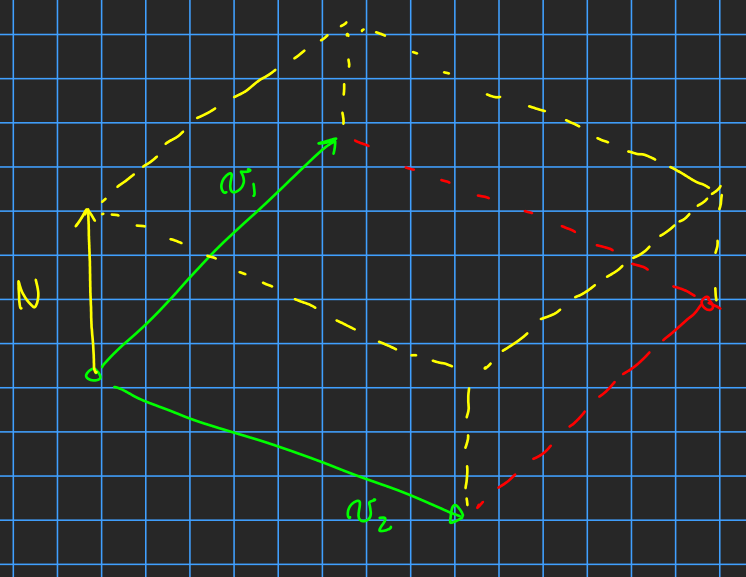
\includegraphics[width=0.8\textwidth, center]{parallelogramma.png}
   	 	\caption{Il parallelogramma immerso in $\RR^3$ e il suo vettore normale $N$.}
   	 	\label{fig:figure3}
   	 \end{figure}
   	 \begin{definition}[Volume non orientato $k$-dimensionale]
   	 	Siano $v_1,\dots,v_k\in\RR^n$ allora il volume non orientato $k$-dimensionale è il valore assoluto del determinante della matrice con colonne $v_1,\dots,v_k,v_{k+1},\dots,v_n$, dove $v_{k+1},\dots,v_{n}$ è una base ortonormale di 
   	 	$$\langle \left\{v_1,\dots,v_k\right\}\rangle^\perp$$
   	 \end{definition}
   	 rimandiamo la discussione sull'unicità e la non dipendenza dalla scelta della base al teorema di Binet-Gram. Nel caso in cui $k=n-1$ abbiamo il molto comodo:
   	 \begin{proposition}[Volume dal prodotto vettoriale]
   	 	Dati $n-1$ vettori $v_1,\dots,v_{n-1}$ in $\RR^n$, il volume non orientato $n-1$ dimensionale del parallelogramma generato da $v_1,\dots,v_{n-1}$ è dato da
   	 	$$\abs{\abs{v_1\times v_2\times \dots \times v_{n-1}}}$$
   	 \end{proposition}
   	 \begin{proof}
   	 	Se $v_1,\dots,v_{n-1}$ sono linearmente indipendenti allora il parallelogramma generato da $v_1,\dots,v_{n-1}$ non è $n-1$ dimensionale, cioè ha volume $n-1$-dimensionale $0$, che corrisponde al fatto che il prodotto vettoriale sia $0$. \\
   	 	D'altra parte se $v_1,v_2,\dots,v_{n-1}$ sono linearmente indipendenti allora $v_1\times v_2\times \dots \times v_{n-1}$ è una base di 
   	 	$$S=\langle \left\{v_1,\dots,v_{n-1}\right\}\rangle^\perp$$
   	 	abbiamo allora solo due basi ortonormali di $S$ (perché $\abs{\abs{\lambda v}}=\abs{\lambda} \abs{\abs{v}}$), ognuna costituita da un solo vettore, scelto tra
   	 	$$v_n=\frac{1}{\abs{\abs{v_1\times v_2 \times \dots \times v_{n-1}}}}(v_1\times v_2 \times \dots \times v_{n-1})$$
   	 	oppure
   	 	$$v_n=\frac{-1}{\abs{\abs{v_1\times v_2 \times \dots \times v_{n-1}}}}(v_1\times v_2 \times \dots \times v_{n-1})$$
   	 	notiamo che ai fini del calcolo del volume non orientato, questi due vettori sono uguali, quindi consideriamo WLOG solo il primo caso. Per definizione di volume $n-1$ dimensionale non orientato abbiamo:
   	 	$$\text{vol}_{n-1}(P(v_1,\dots,v_{n-1}))=\det(v_1,v_2,\dots,v_n)$$
   	 	che per definizione di prodotto vettoriale è proprio
   	 	$$\dots=\langle v_1\times v_2 \times \dots \times v_{n-1},v_n\rangle=\frac{\langle v_1\times v_2 \times \dots \times v_{n-1},v_1\times v_2 \times \dots \times v_{n-1}\rangle}{\abs{\abs{v_1\times v_2 \times \dots \times v_{n-1}}}}=\abs{\abs{v_1\times v_2 \times \dots \times v_{n-1}}}$$
   	 	come volevasi dimostrare.
   	 \end{proof}
   	 Da questo filone di pensiero discende una formula molto famosa per calcolare le aree:
   	 \begin{theorem}[Lagrange/shoelace formula]
   	 	Siano $v_1,\dots,v_{n-1}$ vettori in $\RR^n$. Se $A\in \RR_{(n-1)\times (n-1)}$ è la matrice tale che $A_{ij}=\langle v_i,v_j\rangle$
   	 	$$A=
   	 	\begin{pmatrix}
   	 		\langle v_1, v_1 \rangle & \langle v_1,v_2\rangle & \dots & \langle v_1,v_{n-1} \rangle \\
   	 		\langle v_2, v_1 \rangle & \langle v_2,v_2\rangle & \dots & \langle v_2,v_{n-1} \rangle \\
   	 		\vdots & \vdots & \ddots & \vdots \\
   	 		\langle v_{n-1}, v_1 \rangle & \langle v_{n-1}, v_2\rangle & \dots & \langle v_{n-1},v_{n-1} \rangle
   	 	\end{pmatrix}
   	 	$$
   	 	allora 
   	 	$$\abs{\abs{v_1\times v_2 \times \dots \times v_{n-1}}}^2=\det A.$$
   	 \end{theorem}
   	 \begin{proof}
   	 	Sia 
   	 	$$w:=v_1\times v_2 \times \dots \times v_{n-1}$$
   	 	e sia
   	 	$$u=\frac{w}{\abs{\abs{w}}}.$$
   	 	Il trucco sta nel considerare la matrice $V$ di colonne:
   	 	$$V=\left(
   	 	\begin{array}{c|c|c|c}
   	 		v_1 & v_2 & \dots & v_{n-1} 
   	 	\end{array}
   	 	\right).$$
   	 	chiaramente abbiamo che $V^\intercal V= A$, inoltre se definiamo 
   	 	$$M=\left(
   	 	\begin{array}{c|c}
   	 		V & u
   	 	\end{array}
   	 	\right)$$
   	 	abbiamo che $M$ ha determinante per definizione uguale al volume orientato $n-1$-dimensionale del parallelogramma generato dai vettori $v_i$, cioè è uguale a $\abs{\abs{v_1\times v_2 \times \dots \times v_{n-1}}}$, d'altra parte
   	 	$$M^\intercal M=\left(
   	 	\begin{array}{c|c}
   	 		A & V^\intercal u \\
   	 		\hline
   	 		u^\intercal V & \langle u,u\rangle
   	 	\end{array}
   	 	\right)=\left(
   	 	\begin{array}{c|c}
   	 		A & 0 \\
   	 		\hline
   	 		0 & 1
   	 	\end{array}
   	 	\right)$$
   	 	dove abbiamo annullato i termini sull'orlo perchè per definizione di $u$ abbiamo $\langle v_i,u\rangle=0$ per ogni $i$. Dunque abbiamo
   	 	$$\abs{{v_1\times v_2\times \dots \times v_{n-1}}}^2=\det M^\intercal M=\det A$$
   	 	che era quanto volevamo dimostrare.
   	 \end{proof}
   	 E una naturale generalizzazione per tutti gli altri volumi è:
   	 \begin{theorem}[Binet-Gram]
   	 	Siano $v_1,\dots,v_k$ vettori in $\RR^n$ e sia $G$ la matrice 
   	 	$$G=
   	 	\begin{pmatrix}
   	 		\langle v_1, v_1 \rangle & \langle v_1,v_2\rangle & \dots & \langle v_1,v_{k} \rangle \\
   	 		\langle v_2, v_1 \rangle & \langle v_2,v_2\rangle & \dots & \langle v_2,v_{k} \rangle \\
   	 		\vdots & \vdots & \ddots & \vdots \\
   	 		\langle v_{k}, v_1 \rangle & \langle v_{k}, v_2\rangle & \dots & \langle v_{k},v_{k} \rangle
   	 	\end{pmatrix}
   	 	$$
   	 	allora abbiamo che 
   	 	$$\det G = [\text{vol}_k(P(v_1,\dots,v_k))]^2$$
   	 \end{theorem}
   	 \begin{proof}
   	 	Essenzialmente analoga: prendiamo una base ortonormale $u_i$ del complemento ortogonale $\left\{v_1,v_2,\dots,v_k\right\}^\perp$ chiamiamo 
   	 	$$V:=\left(
   	 	\begin{array}{c|c|c|c}
   	 		v_1 & v_2 & \dots & v_k
   	 	\end{array}
   	 	\right)$$
   	 	e 
   	 	$$U:=\left(
   	 	\begin{array}{c|c|c|c}
   	 		u_{k+1} & v_{k+2} & \dots & u_n
   	 	\end{array}
   	 	\right).$$
   	 	Definiamo nuovamente la matrice 
   	 	$$M:=\left(\begin{array}{c|c}
   	 		V & U
   	 	\end{array}\right)$$
   	 	con determinante uguale (per definizione) al volume orientato $k$-dimensionale del parallelogramma generato dai $v_i$. Allora abbiamo
   	 	$$M^\intercal M = \left(
   	 	\begin{array}{c|c}
   	 		G & V^\intercal U \\
   	 		\hline
   	 		U^\intercal V & U^\intercal U
   	 	\end{array}
   	 	\right)$$
   	 	d'altra parte le colonne di $U$ sono per definizione un insieme ortonormale, quindi $U$ è ortogonale, ovvero $U^\intercal U =I$, inoltre le colonne di $U$ sono per definizione tutte ortogonali a tutte le colonne di $V$, quindi abbiamo semplicemente
   	 	$$U^\intercal V =0$$
   	 	$$V^\intercal U=0$$
   	 	e come prima
   	 	$$\det M^\intercal M = \det\left(
   	 	\begin{array}{c|c}
   	 		G & 0 \\
   	 		\hline
   	 		0 & I
   	 	\end{array}
   	 	\right)=\det G$$
   	 	da cui la tesi.
   	 \end{proof}
   	 
   	 \newpage
   	 
   	 \section{Applicazioni tra spazi euclidei}
   	 
   	 
   	 Finora ci siamo occupati di angoli, norme, ortogonalità e volumi rimanendo sempre dentro allo stesso spazio. Ora, come si fa solitamente quando si definisce una nuova struttura, ci occupiamo di studiare i morfismi e le applicazioni tra spazi euclidei che preservano la struttura. \\
   	 
   	 \subsection{Di nuovo matrici ortogonali}
   	 
   	 Per come abbiamo definito le matrici ortogonali notiamo che, data una matrice $Q$, è più facile calcolare $Q^\intercal Q$ e controllare se sia l'identità (e quindi controllare se $Q$ è ortogonale), che controllare se sia invertibile calcolando $Q^{-1}$. 
   	 \begin{example}[Controllare che una $2\times 2$ è ortogonale]
   	 	Data una matrice 
   	 	$$Q=
   	 	\begin{pmatrix}
   	 		a & b \\
   	 		c & d
   	 	\end{pmatrix}
   	 	$$
   	 	la matrice $Q^\intercal Q$ soddisfa
   	 	$$
   	 	Q^\intercal Q =
   	 	\begin{pmatrix}
   	 		a & c \\
   	 		b & d
   	 	\end{pmatrix}
   	 	\begin{pmatrix}
   	 		a & b \\
   	 		c & d
   	 	\end{pmatrix}
   	 	=
   	 	\begin{pmatrix}
   	 		a^2 + c^2 & ab+cd \\
   	 		ab + cd & b^2+d^2
   	 	\end{pmatrix}
   	 	$$
   	 	quindi se vogliamo che $Q$ sia ortogonale dobbiamo avere
   	 	$$a^2+c^2=1$$
   	 	$$b^2+c^2=1$$
   	 	$$ab+cd=0$$
   	 	in particolare possiamo dimostrare che le uniche matrici che soddisfano questa condizione sono quelle della forma
   	 	$$
   	 	\begin{pmatrix}
   	 		\cos\theta & \sin\theta \\
   	 		-\sin\theta & \cos\theta
   	 	\end{pmatrix},
   	 	\begin{pmatrix}
   	 		\cos\theta & \sin\theta \\
   	 		\sin\theta & -\cos\theta
   	 	\end{pmatrix}.
   	 	$$
   	 \end{example}
   	 \begin{example}[Decomposizione QR]
   	 	Data una matrice $A$ quadrata, troviamo una sua decomposizione QR. Ci basta trovare una base ortonormale di $\RR^n$, scrivere la matrice $Q$ con colonne quei vettori, e calcolare
   	 	$$R=Q^\intercal A$$
   	 	per ottenere la matrice $R$.
   	 \end{example}
   	 
   	 \begin{lemma}[Determinante di una matrice ortogonale]
   	 	Sia $Q$ una matrice ortogonale, allora 
   	 	$$\det Q = \pm 1.$$
   	 \end{lemma}
   	 \begin{proof}
   	 	Semplicemente abbiamo che 
   	 	$$Q^\intercal Q = I$$
   	 	quindi per binet
   	 	$$\det ( Q)\det(Q^\intercal)=1 \iff \left(\det Q\right)^2=1$$
   	 	che implica direttamente la tesi.
   	 \end{proof}
   	 La condizione prima era solo necessaria, la seguente invece è una vera e propria caratterizzazione
   	 \begin{lemma}[Le matrici ortogonali sono isometrie]
   	 	Sia $Q$ una matrice quadrata. Allora $Q$ è ortogonale se e solo se per ogni $v,w\in\RR^n$ vale
   	 	$$\langle Qv,Qw\rangle = \langle v,w \rangle$$
   	 	detto altrimenti la matrice $Q$ \textit{preserva il prodotto scalare}.
   	 \end{lemma}
   	 \begin{proof}
   	 	Se $Q$ è una matrice ortogonale allora possiamo sfruttare la scrittura del prodotto scalare come moltiplicazione per il trasposto:
   	 	$$\langle Qv, Qw\rangle=\left(Qv\right)^\intercal \left(Qw\right)$$
   	 	d'altra parte per una proprietà della trasposizione
   	 	$$\dots=v^\intercal Q^\intercal Q w=v^\intercal w=\langle v,w\rangle.$$
   	 	Viceversa, se $Q$ preserva il prodotto scalre, prendiamo la base canonica $e_1,\dots,e_n$ di $\RR^n$. Abbiamo che
   	 	$$\langle Qe_i,Qe_j\rangle = \langle e_i,e_j \rangle =\delta_{ij}$$
   	 	d'altra parte $Qe_i$ è semplicemente la colonna $i$-esima della matrice $Q$, e $Qe_j$ è semplicemente la colonna $j$-esima della matrice $Q$. Questo ci dice proprio che il prodotto scalare tra colonne distinte di $Q$ restituisce $0$, e il prodotto scalare di ogni colonna con se stessa è $1$, dunque abbiamo che le colonne di $Q$ sono un insieme ortonormale, e abbiamo finito.
   	 \end{proof}
   	 Un'altra proprietà interessante delle matrici ortogonali riguarda gli autovalori:
   	 \begin{lemma}[Autovalori di una matrice ortogonale]
   	 	Sia $Q$ una matrice ortogonale, e sia $\lambda$ un suo autovalore reale. Allora abbiamo $\lambda = \pm 1$.
   	 \end{lemma}
   	 \begin{proof}
   	 	Sia $v$ un autovettore associato a $\lambda$. Abbiamo per quanto appena dimostrato:
   	 	$$\langle Qv,Qv\rangle = \langle v,v\rangle $$
   	 	d'altra parte per definizione di autovettore 
   	 	$$\langle \lambda v,\lambda v \rangle = \langle v,v \rangle $$
   	 	e quindi 
   	 	$$\lambda^2 = 1$$
   	 	che implica la tesi.
   	 \end{proof}
   	 Infine arriviamo al seguente algebroso risultato
   	 \begin{lemma}[Le matrici ortogonali sono un gruppo]
   	 	Se $P,Q$ sono due matrici quadrate ortogonali abbiamo che
   	 	\begin{itemize}
   	 		\item[(i)] La matrice $PQ$ è ancora ortogonale.
   	 		\item[(ii)] La matrice $P^{-1}$ è ancora ortogonale.
   	 	\end{itemize}
   	 \end{lemma}
   	 \begin{proof}
   	 	Il punto (ii) è abbastanza chiaro. Per il punto (i) prendiamo la trasposta di $PQ$:
   	 	$$(PQ)^\intercal=Q^\intercal P^\intercal$$
   	 	quindi usando il fatto che $P,Q$ sono ortogonali
   	 	$$\dots = Q^{-1}P^{-1}=\left(PQ\right)^{-1}$$
   	 	cioè $PQ$ è ortogonale.
   	 \end{proof}
   	 Questo ci fa sorgere vari dubbi, e ci porta a investigare meglio la struttura delle matrici come gruppo:
   	 \begin{definition}[Gruppi di matrici]
   	 	Dato un campo $K$, possiamo definire il suo \textit{gruppo lineare generale}, di ordine $n$ come
   	 	$$\GL_n(K)=\left\{A\in K_{n\times n}:\det A \ne 0\right\}$$
   	 	analogamente definiamo il \textit{gruppo lineare speciale} come
   	 	$$\SL_n(K)=\left\{A\in K_{n\times n}:\det A =1\right\}$$
   	 	in particolare notiamo che per il primo teorema di omomorfismo abbiamo
   	 	$$\faktor{\GL_n(K)}{\SL_n(K)}=K\setminus \left\{0\right\}$$
   	 	grazie all'omomorfismo indotto dalla funzione determinante. 
   	 \end{definition}
   	 Infine per quanto appena visto definiamo
   	 \begin{definition}[Gruppi di matrici ortogonali]
   	 	Su $\RR$ definiamo il \textit{gruppo ortogonale generale} come
   	 	$$\text{O}_n(\RR)=\left\{A\in \RR_{n\times n}:A^\intercal A = I_n\right\}$$
   	 	e analogamente definiamo il \textit{gruppo ortogonale speciale come}
   	 	$$\text{SO}_n(\RR)=\left\{A\in O_n(\RR):\det A = 1\right\}$$
   	 	ovvero
   	 	$$\text{SO}_n(\RR)=\SL_n(\RR)\cap \text{O}_n(\RR)$$
   	 	che come prima può essere visto come il kernel dell'omomorfismo indotto dal determinante. 
   	 \end{definition}
   	 \begin{example}[Rotazioni]
   	 	Prendiamo le matrici ortogonali $2\times 2$. Se il determinante è $1$, abbiamo che non hanno autovalori reali. Congetturiamo allora che le matrici ortogonali con determinante $1$ siano tutte e sole le matrici di rotazione. Prendiamo quindi $R_\phi$ una rotazione di angolo $\phi$ e un vettore in $\RR^2$ scrivibile come
   	 	$$\begin{pmatrix}
   	 		x \\
   	 		y
   	 	\end{pmatrix}=
   	 	\begin{pmatrix}
   	 		r \cos \psi \\
   	 		r \sin \psi
   	 	\end{pmatrix}$$
   	 	dunque applicando la trasformazione 
   	 	$$R_\phi\begin{pmatrix}
   	 		r \cos \psi \\
   	 		r \sin \psi
   	 	\end{pmatrix}=
   	 	\begin{pmatrix}
   	 		r \cos\left( \psi + \phi\right) \\
   	 		r \sin\left( \psi + \phi\right)
   	 	\end{pmatrix}
   	 	$$
   	 	che d'altra parte ci permette di ricavare la matrice di $R_\phi $ imponendo che $(x,y)^\intercal$ fosse un vettore della base canonica. Da questo troviamo proprio
   	 	$$
   	 	\begin{pmatrix}
   	 		\sin \phi &  \cos \phi \\
   	 		-\cos \phi & \sin\phi
   	 	\end{pmatrix}
   	 	$$
   	 	che era proprio una delle due famiglia di matrici ortogonali possibili che avevamo trovato.
   	 \end{example}
   	 \begin{example}[Simmetrie]
   	 	L'esempio sopra ci fa vedere l'interpretazione di una famiglia di matrici ortogonali in $\RR^2$. D'altra parte notiamo che l'altra famiglia è esattamente l'insieme delle simmetrie con asse inclinato di $\theta$, infatti se come prima scriviamo
   	 	$$S_\theta\begin{pmatrix}
   	 		r\cos \psi \\
   	 		r\sin \psi
   	 	\end{pmatrix}=
   	 	\begin{pmatrix}
   	 		r\cos \psi+2(\theta-\psi) \\
   	 		r\sin \psi+2(\theta-\psi)
   	 	\end{pmatrix}$$
   	 	che con un po' di conti usando formule di addizione sottrazione e duplicazione ci riporta alla formula che conoscevamo. 
   	 \end{example}
   	 I calcoli sopra sono un'importante euristica del fatto che \textbf{ogni matrice ortogonale in $2$ dimensioni è scrivibile come composizione di $\le 2$ simmetrie}.
   	 
   	 \subsection{Isometrie e Cartàn-Dieudonne}
   	 
   	 \begin{definition}[Isometria]
   	 	Un'isometria è un'applicazione $f:\RR^n\to\RR^m$ lineare tale che
   	 	$$\langle f(v),f(w)\rangle=\langle v,w\rangle $$
   	 	per ogni $v,w\in \RR^n$.
   	 \end{definition}
   	 Insomma, un'isometria è un'applicazione che preserva gli angoli le norme e le lunghezze. Un'osservazione importante è che se il prodotto scalare in questione non è degenere, allora
   	 \begin{lemma}[Caratterizzazione delle isometrie]
   	 	Sia $f:\RR^n\to\RR^m$ un'applicazione lineare, allora le seguenti tre sono equivalenti:
   	 	\begin{enumerate}
   	 		\item L'applicazione $f$ è un'isometria.
   	 		\item Per ogni $v\in \RR^n$ abbiamo $\abs{\abs{f(v)}}=\abs{\abs{v}}$.
   	 		\item Per ogni insieme ortonormale $v_1,\dots,v_n$, l'insieme $f(v_1),\dots,f(v_n)$ è ancora ortonormale.
   	 	\end{enumerate} 
   	 \end{lemma}
   	 \begin{proof}
   	 	Il fatto che $1$ implichi $2$ segue semplicemente dal considerare 
   	 	$$\abs{\abs{f(v)}}=\langle f(v),f(v)\rangle = \langle v,v \rangle=\abs{\abs{v}}.$$
   	 	Per dimostrare che $2$ implica $1$ lavoriamo con la norma di somme:
   	 	$$\abs{\abs{f(v+w)}}=\abs{\abs{v+w}}$$
   	 	d'altra parte il lato destro si espande semplicemente come
   	 	$$\dots=\abs{\abs{v+w}}=\abs{\abs{v}}+\abs{\abs{w}}+2\langle v,w\rangle$$
   	 	mentre il lato sinistro 
   	 	$$\abs{\abs{f(v)}}+\abs{\abs{f(w)}}+2\langle f(v),f(w)\rangle=\abs{\abs{f(v)+f(w)}}=\abs{\abs{f(v+w)}}=\dots$$
   	 	che, usando il fatto che $\abs{\abs{f(v)}}=\abs{\abs{v}}$ per ogni $v$ ci dà la tesi. \\
   	 	Passando all'affermazione $3$ ora, è chiaro che la prima implichi la terza, infatti se $v_i,v_j$ sono ortonormali abbiamo
   	 	$$\langle f(v_i),f(v_j) \rangle = \langle v_i,v_j \rangle =\delta_{ij}$$
   	 	e quindi anche le immagini saranno ortonormali. D'altra parte è chiaro anche come la terza segua dalla prima, se abbiamo una base ortonormale $e_i$ che si comporta bene rispetto a $f$, per ogni $v,w$ possiamo scrivere
   	 	$$v=v_1e_1+\dots+v_ne_n$$
   	 	$$w=w_1e_1+\dots+w_ne_n$$
   	 	e quindi usando la bilinearità del prodotto scalare giungiamo facilmente alla tesi.
   	 \end{proof}
   	 \begin{lemma}[Le isometrie sono invertibili]
   	 	Comunque data un'isometria $f:\RR^n\to \RR^m$ se il prodotto scalare non è degenere, allora $f$ è iniettiva. 
   	 \end{lemma}
   	 \begin{proof}
   	 	Se $f(v)=0$ abbiamo
   	 	$$\abs{\abs{f(v)}}=\abs{\abs{v}}$$
   	 	quindi abbiamo che 
   	 	$$\abs{\abs{v}}=0$$
   	 	cioè $v=0$, cioè il kernel di $f$ è banale, quindi è invertibile.
   	 \end{proof}
   	 Mettiamo insieme quanto fatto finora:
   	 \begin{lemma}[Le isometrie sono matrici ortogonali]
   	 	Sia $f:\RR^n\to\RR^n$ un'applicazione lineare. Allora $f$ è un'isometria se e solo se la sua matrice nella base canonica $M_{E}^E(f)$ è ortogonale. 
   	 \end{lemma}
   	 \begin{proof}
   	 	Bruto calcolo, prendiamo $f$, la sua matrice $A$ ed $e_i$ la base canonica. Abbiamo
   	 	$$\langle f(e_i),f(e_j)\rangle = \langle Ae_i,Ae_j \rangle$$
   	 	d'altra parte $Ae_i$ è la colonna $i$ della matrice $A$, e $Ae_j$ è la colonna $j$. Si vede chiaramente quindi che se $A$ è ortogonale abbiamo
   	 	$$\langle Ae_i,Ae_j\rangle = \delta_{ij}$$
   	 	da cui $f$ isometria, e se $f$ è isometria abbiamo
   	 	$$\langle f(e_i),f(e_j) \rangle = \delta_{ij}$$
   	 	da cui $A$ è ortogonale.
   	 \end{proof}
   	 Da questo risultato discende che gli autovalori di un'isometria possono essere solo $\pm 1$. In un certo senso dobbiamo immaginare le isometrie come rotazioni o riflessioni dell'origine, e il prossimo risultato ci chiarirà bene in che senso. Prima abbiamo bisogno del seguente lemma preparatorio: 
   	 \begin{lemma}[Gli spazi stabili si comportano bene rispetto all'ortogonale]
   	 	Sia $f:\RR^n\to\RR^n$ un'isometria. Se $V$ è uno spazio stabile rispetto a $f$, allora 
   	 	$$f\left(V^\perp\right)=V^\perp$$
   	 \end{lemma}
   	 \begin{proof}
   	 	Dati $v\in V$ e $w\in V^\perp$ vogliamo dimostrare che $f(w)$ è di nuovo ortogonale a $V$, cioè
   	 	$$\langle v,f(w)\rangle =0$$
   	 	per ogni $v,w$. Se $V$ è stabile rispetto a $f$ abbiamo $f(V)\subseteq V$ d'altra parte dato che $f$ è un'isometria abbiamo che $f$ è biettiva, quindi $f(V)=V$. Dunque possiamo sempre trovare uno e un solo $v'$ tale che
   	 	$$f(v'))=v \qquad \forall v\in V$$
   	 	dunque 
   	 	$$\langle v,f(w)\rangle = \langle f(v'),f(w)\rangle = \langle v',w \rangle = 0$$
   	 	dove l'ultimo prodotto scalare è $0$ in quanto $v'\in V$ e $w\in V^\perp$.
   	 \end{proof}
   	 \begin{remark}[Volumi]
   	 	Una isometria preserva i volumi non orientati, dato che ha determinante $\pm 1$.
   	 \end{remark}
   	 Finalmente quindi arriviamo al fatto che avevamo acennato e congetturato su $\RR^2$, cioè che ogni isometria può essere decomposta come prodotto di simmetrie:
   	 \begin{theorem}[Cartàn-Dieudonne]
   	 	Sia $f:\RR^n\to\RR^n$ un'isometria. Chiamiamo l'\textit{asse} di $f$ l'autospazio $W$ dell'autovalore $\lambda=1$. Allora abbiamo che $f$ è esprimibile come composizione di al più $n-\dim W$ simmetrie con assi iperpiani di dimensioni $n-1$. 
   	 \end{theorem}
   	 \begin{proof}
   	 	Procediamo per induzione su $c:=n-\dim W$. Se $c=1$ abbiamo che $\dim W=n-1$, ma questo implica che l'ortogonale $W^\perp$ ha dimensione $1$, ma dato che $f$ è stabile su $W$, sarà stabile anche su $W^\perp$. Questo significa che $f$ è proprio un endomorfismo di $W^\perp$, che è uno spazio vettoriale unidimensionale, quindi esisterà un $\lambda$ tale che per ogni $w\in W^\perp$ abbiamo
   	 	$$f(w)=\lambda w$$
   	 	ma allora $W^\perp$ è un autospazio di $f$, che può avere solo autovalori $\pm 1$, e $\lambda$ non può essere $1$ perché abbiamo detto che $W$ è l'autospazio di $1$. Dunque abbiamo che 
   	 	$$f(w)=-w \qquad \forall w\in W^\perp$$
   	 	cioè abbiamo proprio che $f$ è la simmetria 
   	 	$$f(v)=\sigma_{W}^{W^\perp}(v)=:\sigma^\perp_W(v) \qquad \forall v\in \RR^n.$$
   	 	Supponiamo ora per induzione che la tesi valga per un certo $c\ge 1$, dimostriamo che possiamo decomporre $f$ come
   	 	$$f= \sigma_V^\perp\circ g$$
   	 	dove $V$ è un certo spazio $n-1$ dimensionale, $g$ ha autospazio di dimensione maggiore di $\dim W$, dunque avrà un $c$ minore, e quindi per ipotesi induttiva la possiamo fattorizzare in simmetrie.
   	 	\begin{figure}[h]
   	 		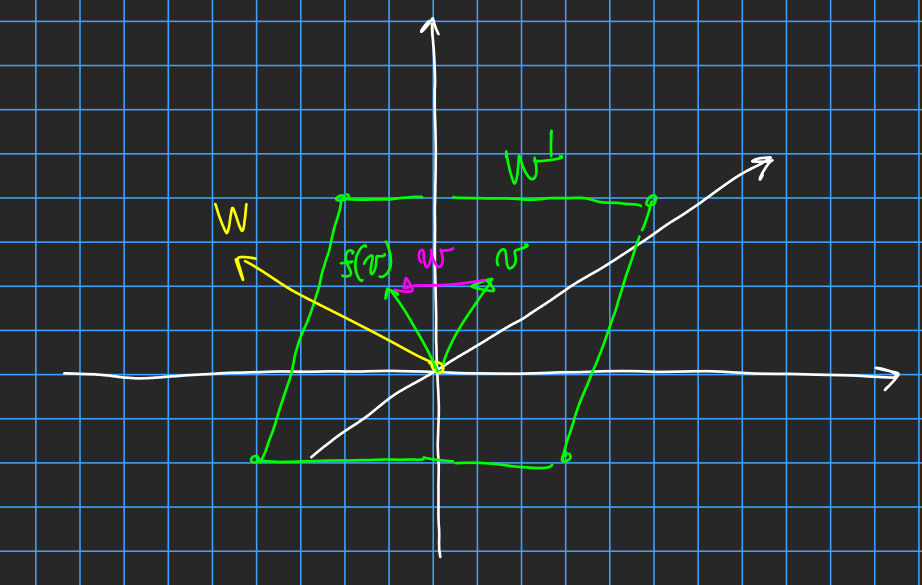
\includegraphics[width=0.8\textwidth, center]{cartan-dieudonne.png}
   	 		\caption{La costruzione del vettore $w$ per il passo induttivo della dimostrazione di Cartàn-Dieudonne nel caso $n=3$ e $\dim W=1$.}
   	 		\label{fig:figure4}
   	 	\end{figure} 
   	 	\\La costruzione è come segue: prendiamo un $v\in W^\perp$ e consideriamo il vettore
   	 	$$w:=f(v)-v$$
   	 	che è sicuramente diverso da $0$ in quanto $v$ è fuori dall'autospazio di $1$. La simmetria che usiamo per fattorizzare $f$ a questo punto è proprio quella di iperpiano 
   	 	$$V:=\left\{w\right\}^\perp$$ 
   	 	grazie al fatto che $\sigma_V^\perp\circ \sigma_V^\perp=\text{id}_{\RR^n}$ possiamo definire $g$ come
   	 	$$g:=\sigma_V^\perp \circ f$$
   	 	il che è evidentemente equivalente a
   	 	$$f=\sigma_V^\perp \circ g.$$
   	 	Per chiudere dunque vogliamo dimostrare due cose:
   	 	\begin{claim}
   	 		L'asse di $g$ contiene $W$.
   	 	\end{claim}
   	 	\begin{subproof}[Sottodimostrazione]
   	 		Consideriamo un $u\in W$, per definizione di $g$ abbiamo
   	 		$$g(u):=\sigma_V^\perp\left(f(u)\right)=\sigma_V^\perp\left(u\right).$$
   	 		D'altra parte osserviamo che $w\in W^\perp$, infatti $W$ è uno spazio $f$-stabile, quindi $f(W^\perp)=W^\perp$ ovvero $f(v)\in W^\perp$ e cioè $f(v)-v\in W^\perp$. Questo vuol dire che 
   	 		$$u\in \left\{w\right\}^\perp=V$$
   	 		e quindi $\sigma_V^\perp(u)=u$, cioè $g(u)=u$ che era la tesi.
   	 	\end{subproof}
   	 	\begin{claim}
   	 		L'asse di $g$ ha dimensione strettamente maggiore di $W$.
   	 	\end{claim}
   	 	\begin{subproof}
   	 		Geometricamente immaginando l'isometria come una rotazione dello spazio $W^\perp$ possiamo guessare che un autovettore fuori da $W$ sia $v$. Dobbiamo allora dimostrare 
   	 		$$\sigma_V^\perp(f(v))=v$$
   	 		d'altra parte per l'algoritmo di Gram-Schmidt possiamo scrivere 
   	 		$$f(v)=\frac{\langle f(v),w\rangle}{\langle w,w\rangle}w+k$$
   	 		per un certo $k\in V$, dunque abbiamo per definizione di $\sigma$
   	 		$$\sigma_V^\perp(f(v))=-\frac{\langle f(v),w\rangle}{\langle w,w\rangle}w+k.$$
   	 		Dato che $f(v)=v+w$ calcoliamo quel coefficiente
   	 		$$\frac{\langle f(v),w\rangle}{\langle w,w\rangle}=\frac{\langle v+w,w\rangle}{\langle w,w\rangle}=1+\frac{\langle v,w\rangle}{\langle w,w\rangle}$$
   	 		e abbiamo
   	 		$$v+w=f(v)=\left(1+\frac{\langle v,w\rangle}{\langle w,w\rangle}\right)w+k$$
   	 		$$v=\frac{\langle v,w\rangle}{\langle w,w\rangle}w+k.$$
   	 		Dunque per dimostrare la tesi non resta che dimostrare che la scomposizione di $v$ è la stessa della riflessione di $\sigma_V^\perp(f(v))$, ovvero
   	 		\begin{gather*}
   	 			-\frac{\langle f(v),w\rangle}{\langle w,w\rangle}=\frac{\langle v,w\rangle}{\langle w,w\rangle} \\
   	 			-\langle f(v),w\rangle=\langle v,w\rangle \\
   	 			\langle f(v),v-f(v)\rangle=\langle v,f(v)-v\rangle \\
   	 			\langle f(v),v\rangle-\langle f(v),f(v)\rangle=\langle f(v),v\rangle-\langle v,v\rangle \\
   	 			\langle f(v),f(v)\rangle=\langle v,v\rangle
   	 		\end{gather*}
   	 		che è una delle caratterizzazioni delle isometrie, e quindi abbiamo finito.
   	 	\end{subproof}
   	 	Abbiamo dimostrato che l'asse di $g$ ha dimensione strettamente maggiore di $W$ e quindi abbiamo finito per ipotesi induttiva.
   	 \end{proof}
   	 \subsection{Mappe lineari conformi}
   	 Un'altra strada per definire applicazioni che preservano la struttura degli spazi Euclidei è quella delle mappe conformi:
   	 \begin{definition}[Mappa conforme]
   	 	Una \textit{mappa conforme} è un'applicazione lineare $f:V\to U$ tra due spazi euclidei tale che $f$ è iniettiva e
   	 	$$\frac{\langle f(v),f(w)\rangle}{\abs{\abs{f(v)}}\abs{\abs{f(w)}}}=\frac{\langle v,w\rangle}{\abs{\abs{v}}\abs{\abs{w}}}$$
   	 	per ogni $v,w\in V$ diversi da $0$. Intuitivamente, vedendo il prodotto scalare come il prodotto delle norme per il coseno dell'angolo tra i vettori, questo vuol dire proprio che la mappa preserva gli angoli.
   	 \end{definition}
   	 \'E chiaro che questa non preservi completamente la struttura dello spazio, tuttavia rimane interessante per molti motivi.
   	 \begin{example}
   	 	Se $f$ è un'isometria, $f$ è anche conforme.
   	 \end{example}
   	 \begin{example}
   	 	Se $f:\RR^n \to \RR^n$ è tale che
   	 	$$f(v)=\alpha v$$
   	 	allora $f$ è conforme. 
   	 \end{example}
   	 Nella definizione di conforme abbiamo assunto che $f(v)$ e $f(w)$ non siano mai zero (a meno che $v$ o $w$ siano $0$), dimostriamo che questo è effettivamente sempre verificato: 
   	 \begin{lemma}[Conforme implica kernel banale]
   	 	Una mappa $f:V\to U$ lineare e conforme è anche iniettiva.
   	 \end{lemma}
   	 \begin{proof}
   	 	Prendiamo due $v,w\in V$ tali che $f(v)=f(w)=k$. Per definizione di conforme abbiamo
   	 	$$1=\frac{\abs{\abs{k}}^2}{\abs{\abs{k}}^2}=\frac{\langle f(v),f(w)\rangle}{\abs{\abs{f(v)}}\abs{\abs{f(w)}}}=\frac{\langle v,w\rangle}{\abs{\abs{v}}\abs{\abs{w}}}$$
   	 	ovvero rigirando un po' i termini
   	 	$$\abs{\abs{v}}\abs{\abs{w}}=\langle v,w\rangle$$
   	 	che per Cauchy-Schwarz vuol dire che esiste uno scalare $\lambda\ne 0$ tale che
   	 	$$v=\lambda w$$
   	 	e quindi abbiamo per linearità
   	 	$$f(w)=f(v)=\lambda f(w) \implies \lambda=1$$
   	 	che era la tesi.
   	 \end{proof}
   	 \begin{proposition}[Caratterizzazioni delle mappe conformi]
   	 	Sia data una $f:\RR^n\to\RR^n$ lineare. Le seguenti proposizioni sono equvalenti:
   	 	\begin{enumerate}
   	 		\item $f$ è conforme.
   	 		\item Per ogni coppia $v,w\in \RR^n$ abbiamo che $\langle v,w\rangle=0$ se e solo se $\langle f(v),f(w)\rangle=0$.
   	 		\item Esiste un $\alpha\ne 0\in \RR$ tale che per ogni coppia $v,w\in \RR^n$ abbiamo
   	 		$$\langle f(v),f(w)\rangle = \alpha^2 \langle v,w \rangle.$$
   	 		\item Esiste un $\alpha\ne 0\in \RR$ tale che per ogni $v\in \RR^n$ vale
   	 		$$\abs{\abs{f(v)}}=\alpha \abs{\abs{v}}.$$
   	 	\end{enumerate}
   	 \end{proposition}
   	 \begin{proof}
   	 	Il fatto che $1$ implichi $2$ segue facilmente dalla definizione di mappa conforme. Notiamo inoltre che $3$ e $4$ sono equivalenti: 
   	 	\begin{description}
   	 		\item[3 $\implies$ 4:] Semplicemente scegliendo $v=w$ abbiamo
   	 		$$\abs{\abs{f(v)}}^2=\alpha^2\abs{\abs{v}}^2$$
   	 		che prendendo le radici ci dà la condizione $4$.
   	 		\item[4 $\implies$ 3:] Abbiamo che per ogni $v,w\in \RR^n$ vale
   	 		$$\langle f(v+w),f(v+w)\rangle=\alpha^2 \abs{\abs{v+w}}$$
   	 		che espandendo con le varie bilinearità diventa
   	 		$$\abs{\abs{f(v)}}^2+\abs{\abs{f(w)}}^2+2\langle f(v),f(w) \rangle=\alpha^2\left(\abs{\abs{v}}^2+\abs{\abs{w}}^2+2\langle v,w\rangle\right)$$
   	 		da cui, espandendo e cancellando i termini che non ci interessano grazie al fatto che $\abs{\abs{f(v)}}=\alpha \abs{\abs{v}}$, ci dà la tesi. 
   	 	\end{description}
   	 	Evidentemente la $3$ implica la $1$. Rimane da dimostrare che la $2$ implica la $4$. Prendiamo due vettori $v,w$ non perpendicolari in $\RR^n$. Allora esisterà un $\alpha\ne 0\in \RR$ tale che 
   	 	$$\langle v,w\rangle -\alpha \langle v,v\rangle=0 \iff \frac{\langle v,w \rangle}{\langle v,v\rangle}=\alpha$$
   	 	cioè per bilinearità e per la condizione $2$ abbiamo
   	 	$$\langle w-\alpha v, v\rangle=0 \iff \langle f(w-\alpha v),f(v)\rangle=0$$	
   	 	ma questo di nuovo per la bilinearità del prodotto e per la linearità di $f$ ci dà
   	 	$$\frac{\langle f(v),f(w) \rangle}{\langle f(v),f(v)\rangle }=\alpha$$
   	 	ovvero, uguagliando gli $\alpha$ e riarrangiando un po' i termini
   	 	$$\frac{\langle f(v),f(w)\rangle}{\langle v,w\rangle}=\frac{\langle f(v),f(v)\rangle}{\langle v,v\rangle}$$
   	 	che d'altra parte per la simmetria è anche uguale a 
   	 	$$\frac{\langle f(v),f(v)\rangle}{\langle v,v\rangle}=\frac{\langle f(v),f(w)\rangle}{\langle v,w\rangle}=\frac{\langle f(w),f(w)\rangle}{\langle w,w\rangle}$$
   	 	insomma, abbiamo dimostrato che per ogni $v\in \RR^n$ il rapporto che stiamo considerando è costante, chiamiamolo $\beta$:
   	 	$$ \frac{\abs{\abs{f(v)}}^2}{\abs{\abs{v}}^2}=\beta $$
   	 	che implica immediatamente la $4$.
   	 \end{proof}
   	 
   	 \begin{definition}[Indice di conformità]
   	 	Per una mappa conforme, il numero $\alpha\in\RR$ tale che per ogni $v$ vale
   	 	$$\abs{\abs{f(v)}}=\alpha \abs{\abs{v}}$$
   	 	si dice \textit{indice di conformità}.
   	 \end{definition}
   	 Il seguente risultato è chiaro, per cui non lo dimostreremo, però è notevole, e quindi lo eleviamo allo status di lemma:
   	 \begin{lemma}[Matrice di una mappa conforme]
   	 	Data una mappa conforme $f:\RR^n\to\RR^n$ la sua matrice rispetto alla base canonica è $A$ tale che
   	 	$$\left(A^\intercal A\right)_{ij} =\alpha^2\delta_{ij}$$
   	 	ovvero
   	 	$$A^\intercal A = \alpha^2 I_n$$
   	 	dove $\alpha$ è l'indice di conformità di $f$. In particolare dunque si ha
   	 	$$\det(A)^2=\alpha^{2n}$$
   	 	e quindi
   	 	$$\det A = \pm \alpha^n.$$
   	 \end{lemma}
   	 da questo segue facilmente che una mappa conforme con indice di conformità $1$ è un'isometria.
   	 
   	 \begin{lemma}[Autovalori di una mappa conforme]
   	 	Una mappa conforme $f:\RR^n\to\RR^n$ con indice di conformità $\alpha$ ha solo autovalori con modulo $\alpha$.
   	 \end{lemma}
   	 \begin{proof}
   	 	Per il lemma precedente abbiamo che la matrice di $f$ rispetto alla base canonica è
   	 	$$A^\intercal A = \alpha^2I_n$$
   	 	ma questo vuol dire che
   	 	$$\left(\frac{A}{\alpha}\right)^\intercal\left(\frac{A}{\alpha}\right)=I_n$$
   	 	ovvero $A/\alpha$ è un'isometria. Prendiamo allora un autovettore $v$ e un suo autovalore $\lambda$ di $A$, questi soddisfano
   	 	$$Av=\lambda v$$
   	 	e dividendo da ambo i lati per $\alpha$ 
   	 	$$\left(\frac{A}{\alpha}\right)v=\left(\frac{\lambda}{\alpha}\right)v$$
   	 	cioè $v$ è un autovettore di un'isometria con autovalore $\lambda/\alpha$, che deve necessariamente essere $\pm 1$, da cui la tesi.
   	 \end{proof}
   	 \newpage
   	 
   	 \section{Spazi Hermitiani}
   	 
   	 Sullo spazio $\RR^n$ avevamo definito il prodotto scalare come una forma bilineare simmetrica tale che
   	 $$\langle v,w\rangle=v^\intercal w$$
   	 per tutti i $v,w$. Estendere naturalmente questa cosa a $\CC$ non è così semplice, infatti se identificassimo brutalmente $\CC$ con $\RR^2$ otterremmo facilmente vettori con norma $0$ che non dovrebbero averla, si pensi a
   	 $$
   	 z=\begin{pmatrix}
   	 	1 \\
   	 	i
   	 \end{pmatrix}
   	 $$
   	 che soddisfa la problematica $z^\intercal z = 0$. Dunque vogliamo introdurre una naturale generalizzazione del prodotto scalare tale che se $v,w\in \RR^n$ si abbia
   	 $$\langle v,w\rangle_{\RR^n}=\langle v,w\rangle_{\CC^n}$$
   	 e inoltre tale che la norma si comporti bene come su $\RR$, cioè
   	 $$\langle v,v\rangle_{\CC^n}=\abs{\abs{v}}_{\CC^n}=\abs{\abs{v}}_{\RR^{2n}}=\langle v,v \rangle_{\RR^{2n}}$$
   	 questo ci porta a definire proprio 
   	 \begin{definition}[Prodotto Hermitiano standard]
   	 	dati due vettori $v,w\in\CC^n$ si definisce il \textit{prodotto hermitiano standard} la seguente operazione $\langle \cdot,\cdot \rangle:\CC^n\times \CC^n\to \RR^n$:
   	 	$$\left\langle
   	 	\begin{pmatrix}
   	 		v_1 \\
   	 		v_2 \\
   	 		\vdots \\
   	 		v_n
   	 	\end{pmatrix},
   	 	\begin{pmatrix}
   	 		w_1 \\
   	 		w_2 \\
   	 		\vdots \\
   	 		w_n
   	 	\end{pmatrix}
   	 	\right\rangle=
   	 	\sum_{i=1}^{n}\overline{v}_iw_i
   	 	$$
   	 	dove la sbarra indica il coniugato complesso. Uno spazio vettoriale dotato di un prodotto Hermitiano si dice \textit{spazio hermitiano}.
   	 \end{definition}
   	 Il primo grosso problema di questo prodotto è che non è simmetrico, infatti si ha
   	 \begin{lemma}[Proprietà del prodotto hermitiano standard]
   	 	Dati due $v,w\in\CC^n$ e $\lambda\in \CC$ si ha
   	 	\begin{itemize}
   	 		\item $\langle v,w\rangle = \overline{\langle w,v\rangle}$.
   	 		\item $\langle \lambda v,w\rangle = \overline{\lambda}\langle v,w\rangle$.
   	 		\item $\langle v,\lambda w\rangle = \lambda \langle v,w\rangle$.
   	 		\item $\langle v+u,w\rangle = \langle v,w\rangle + \langle u,w\rangle$.
   	 		\item Se per ogni $z\in \CC$ vale $\langle v,z\rangle =0$ allora $v=0$.
   	 		\item La \textit{norma} di $w$ è definita come $\langle w,w\rangle$, che è sempre maggiore o uguale a $0$, ed in particolare è zero se e solo se $w=0$.
   	 	\end{itemize}
   	 \end{lemma}
   	 \begin{proof}
   	 	Conti.
   	 \end{proof}
   	 Praticamente tutti i risultati dimostrati finora possono essere generalizzati al caso hermitiano, sotto le opportune ridefinizioni. I risultati della sezione $9.1$ possono facilmente essere ricondotti al caso hermitiano. Quello che non è davvero chiaro è come cambi il concetto di matrice ortogonale, per fare ciò dobbiamo dare prima un po' di definizioni.
   	 
   	 \subsection{Classi di matrici generali}
   	 
   	 \begin{definition}[Matrice aggiunta]
   	 	Data una matrice $A\in\CC_{m\times n}$, si definisce la sua matrice \textit{aggiunta}, la matrice $$A^*:=\overline{A}^\intercal.$$ 
   	 \end{definition}
   	 L'aggiunta soddisfa tutte le proprietà che ci aspettiamo dalla trasposta:
   	 \begin{lemma}[Proprietà dell'aggiunta]
   	 	Date due matrici $A,B$ a coefficienti in $\CC$ abbiamo che:
   	 	\begin{itemize}
   	 		\item $\left(AB\right)^*=B^*A^*$.
   	 		\item $\det A^*=\overline{\det A}$.
   	 		\item $\rank{A}=\rank{A^*}$.
   	 		\item $\left(A^{-1}\right)^*=\left(A^*\right)^{-1}$.
   	 	\end{itemize} 
   	 \end{lemma}
   	 \begin{proof}
   	 	Dimostriamo una cosa alla volta:
   	 	\begin{itemize}
   	 		\item Dalla definizione di aggiunta e dal fatto che il coniugato è moltiplicativo segue facilmente che
   	 		$$\left(AB\right)=\overline{AB}^\intercal=\left(\overline{A}\overline{B}\right)^\intercal=\overline{B}^\intercal \overline{A}^\intercal=B^*A^*.$$
   	 		\item Segue abbastanza chiaramente dal fatto che $\det A=\det A^\intercal$ e dal fatto che il coniugato distribuisce su somme e prodotti (unito alla formula esplicita per il determinante).
   	 		\item Dal teorema dei minori orlati e dal fatto che $\det A^*=\overline{\det A}$.
   	 		\item Dobbiamo dimostrare che $A^*$ è l'inversa di $\left(A^{-1}\right)^*$. D'altra parte per quanto mostrato prima
   	 		$$\left(A^{-1}\right)^*A^*=\left(AA^{-1}\right)^*=I_n^*=I_n$$
   	 		e dunque per l'unicità dell'inversa abbiamo finito.
   	 	\end{itemize}
   	 	Dunque abbiamo ottenuto tutte le tesi, e abbiamo finito.
   	 \end{proof}
   	 
   	 Ma il vero motivo per cui abbiamo definito così l'aggiunta è che ora comunque dati due vettori $v,w\in\CC$ abbiamo
   	 $$\langle v,w\rangle = v^*w.$$
   	 Questa condizione è espressa sinteticamente nel seguente lemma:
   	 \begin{lemma}[Definizione di operatore aggiunto]
     Data una matrice\footnote{In realtà qui potremmo parlare anche di operatore generico.}  $A\in \CC_{n\times m}$ la sua matrice aggiunta è l'unica matrice in $\CC_{m\times n}$ tale che per ogni $v\in \CC^m$ e $w\in \CC^n$ vale
   	 $$\langle Av,w\rangle = \langle v,A^*w\rangle.$$
   	 \end{lemma}
   	 \begin{proof}
   	 	Un verso è facile, infatti abbiamo che
   	 	$$\langle Av,w\rangle=\left(Av\right)^* w=v^*A^*w=\langle v,A^*w\rangle$$
   	 	e quindi abbiamo proprio che la matrice aggiunta soddisfa quell'identità. L'altro verso è più complicato: se una certa matrice $B$ è tale che per ogni $v,w\in \CC^n$ si abbia
   	 	$$\langle Av,w\rangle=\langle v,Bw\rangle$$
   	 	allora scegliendo $v=e_i$ e $w=e_j$, i vettori della base canonica, abbiamo
   	 	$$\langle Ae_i,e_j\rangle=\overline{A}_{ji}$$
   	 	$$\langle e_i,Be_j\rangle=B_{ij}$$
   	 	ovvero per ogni $i,j$ 
   	 	$$\overline{A}_{ji}=B_{ij}$$
   	 	il che vuol dire proprio che $B$ è la trasposta coniugata di $A$, cioè la sua aggiunta.
   	 \end{proof}
   	 Questo ci permette di nuovo di scrivere sinteticamente la coppia $V, V^\perp$, per ogni sottospazio $V$ di $\CC^n$ con una matrice formata ponendo sulle colonne una base di $V$: 
   	 $$A=\left(\begin{array}{c|c|c|c}
   	 	v_1 & v_2 & \dots & v_k
   	 \end{array}\right)$$
   	 in questo modo abbiamo di nuovo che
   	 $$\ker{A^*}=V^\perp$$
   	 $$\Immagine{A}=V$$
   	 come avevamo già visto nel caso reale. Allo stesso modo abbiamo, come visto nella sezione $9.2$ che la matrice di una proiezione ortogonale su uno spazio vettoriale $V$ è 
   	 $$A\left(A^* A\right)^{-1}A^*$$ 
   	 dove $A$ è la matrice avente per colonne una base di $V$. Analogamente si dimostrano anche Gram-Schmidt e la decomposizione $QR$ (sostituendo a tutte le trasposte le aggiunte). Generalizziamo anche il concetto di matrice simmetrica e ortogonale:
   	 \begin{definition}[Matrici Hermitiane, Normali e Unitarie]
   	 	Una matrice $A$ si dice \textit{Hermitiana} se soddisfa
   	 	$$A^*=A$$
   	 	si dice \textit{unitaria} se le sue colonne sono un insieme ortonormale rispetto al prodotto, hermitiano, ovvero
   	 	$$AA^*=A^*A=I_n$$
   	 	infine una matrice si dice \textit{normale}, se commuta con la sua aggiunta, ovvero
   	 	$$A^*A=AA^*.$$
   	 	Chiaramente abbiamo che hermitiana o unitaria implicano normale. Inoltre notiamo che tutte le matrici normali sono quadrate.
   	 \end{definition}
   	 \begin{definition}[Gruppi unitari generali e speciali]
   	 	In $\CC_{n\times m}$ definiamo il \textit{gruppo unitario generale} delle matrici quadrate unitarie e lo denotiamo con $\text{U}_n(\CC)$. Analogamente definiamo il \textit{gruppo unitario speciale}, delle matrici quadrate unitarie con determinante $1$, e lo denotiamo con $\text{SU}_n(\CC)$.
   	 \end{definition}
   	 Cominciamo a generalizzare alcuni risultati che abbiamo già visto per gli spazi euclidei:
   	 \begin{lemma}[Determinante di una matrice unitaria]
   	 	Sia $A\in \text{U}_n(\CC)$, allora abbiamo $\abs{\det A}=1$ (notiamo che di solito il determinante sarà un numero complesso).
   	 \end{lemma}
   	 \begin{proof}
   	 	Per definizione di matrice unitaria abbiamo
   	 	$$1=\det\left(A^* A\right)=\det A^* \det A=\det\overline{A}\det A=\overline{\det A}\det A$$
   	 	e quindi 
   	 	$$\abs{\det A}^2=1$$
   	 	che implica la tesi.
   	 \end{proof}
   	 \begin{example}[Matrici unitarie con determinante arbitrario]
   	 	Consideriamo la matrice
   	 	$$A=\begin{pmatrix}
   	 		e^{i\theta} & 0 \\
   	 		0 & 1
   	 	\end{pmatrix}$$
   	 	con $\theta\in\RR$ arbitrario. Questa ha determinante
   	 	$$\det A=e^{i\theta}$$
   	 	e inoltre è unitaria, infatti
   	 	$$A^*A=\begin{pmatrix}
   	 		e^{-i\theta} & 0 \\
   	 		0 & 1
   	 	\end{pmatrix}
   	 	\begin{pmatrix}
   	 		e^{i\theta} & 0 \\
   	 		0 & 1
   	 	\end{pmatrix}
   	 	=
   	 	\begin{pmatrix}
   	 		1 & 0 \\
   	 		0 & 1
   	 	\end{pmatrix}.
   	 	$$
   	 \end{example}
   	 \begin{lemma}[Autovalori di una matrice unitaria]
   	 	Sia $A\in \text{U}_n(\CC)$ e $\lambda$ un suo autovalore. Allora $\abs{\lambda}=1$.
   	 \end{lemma}
   	 \begin{proof}
   	 	Prendiamo un autovalore $\lambda$ di $A$ e un suo autovettore $v$, abbiamo per definizione
   	 	$$Av=\lambda v$$
   	 	d'altra parte abbiamo
   	 	$$\langle Av,v \rangle = \langle v,A^*v\rangle$$
   	 	e inoltre
   	 	$$A^*v=A^{-1}v=\frac{v}{\lambda}$$
   	 	il che ci porta a dire che 
   	 	$$\overline{\lambda}\langle v,v\rangle=\dots=\frac{1}{\lambda}\langle v,v\rangle$$
   	 	cioè
   	 	$$\overline{\lambda}\lambda=1$$
   	 	che implica la tesi.
   	 \end{proof}
   	 \begin{proposition}[Proprietà delle matrici normali]
   	 	Sia $A$ una matrice normale, allora:
   	 	\begin{enumerate}
   	 		\item Per ogni $v\in\CC^n$ si ha $\abs{\abs{A v}}=\abs{\abs{A^*v}}$.
   	 		\item Per ogni $\lambda\in \CC$ abbiamo che $A-\lambda I_n$ è normale.
   	 		\item Se $v$ è un autovettore di $A$ di autovalore $\lambda$, allora $v$ è un autovettore di $A^*$ con autovalore $\overline{\lambda}$.
   	 		\item Se $v,w$ sono autovettori di $A$ relativi ad autovalori distinti allora $\langle v,w\rangle =0$. 
   	 	\end{enumerate}
   	 \end{proposition}
   	 \begin{proof}
   	 	Dimostriamo una cosa alla volta:
   	 	\begin{enumerate}
   	 		\item \'E un calcolo esplicito. Facciamo
   	 		$$\abs{\abs{Av}}=\left(Av\right)^*Av=v^*A^*Av$$
   	 		ma dato che $A$ è normale abbiamo
   	 		$$\dots=v^*AA^*v=\abs{\abs{A^*v}}$$
   	 		come richiesto.
   	 		\item Anche qui un calcolo esplicito:
   	 		$$\left(A-\lambda I_n\right)\left(A-\lambda I_n\right)^*=\left(A-\lambda I_n\right)\left(A^*-\overline{\lambda}I_n\right)$$
   	 		ora sviluppando i prodotti:
   	 		$$\dots=AA^*-\lambda A^*-\overline{\lambda}A+\lambda \overline{\lambda}I_n$$
   	 		mentre sviluppando l'altro prodotto otteniamo
   	 		$$\left(A-\lambda I_n\right)^*\left(A-\lambda I_n\right)=A^*A-\lambda A^*-\overline{\lambda}A+\lambda \overline{\lambda}I_n$$
   	 		e quindi dato che $A$ è normale le due espressioni sono uguali.
   	 		\item Conseguenza dei due punti precedenti. Prendiamo un autovettore $v$ di autovalore $\lambda$ di $A$, allora
   	 		$$\left(A-\lambda I_n\right)v=0$$
   	 		ma ora sappiamo due cose, la prima è che per il punto $2$ la matrice $A-\lambda I_n$ è normale, e la seconda è che per il punto $1$ sappiamo che
   	 		$$0=\abs{\abs{0}}=\abs{\abs{\left(A-\lambda I_n\right)v}}=\abs{\abs{\left(A-\lambda I_n\right)^*v}}$$
   	 		cioè abbiamo che 
   	 		$$\left(A-\lambda I_n\right)^*v=0$$
   	 		ovvero
   	 		$$\left(A^*-\overline{\lambda}I_n\right)v=0$$
   	 		cioè $v$ è un autovettore di $A^*$ di autovalore $\overline{\lambda}$.
   	 		\item Conseguenza del punto precedente. Prendiamo un autovettore $v$ di autovalore $\lambda$ e un autovettore $w$ di autovalore $\mu$ con $\mu\ne \lambda$, abbiamo
   	 		$$\lambda \langle v,w\rangle = \langle \overline{\lambda}v,w\rangle$$
   	 		d'altra parte per il punto precedente sappiamo che $v$ è un autovettore di $A^*$ con autovalore $\overline{\lambda}$, quindi
   	 		$$\lambda\langle v,w\rangle=\dots = \langle A^*v,w\rangle= \langle v,Aw\rangle=\mu \langle v,w\rangle$$
   	 		da cui
   	 		$$(\lambda-\mu)\langle v,w\rangle=0$$
   	 		cioè $v,w$ sono perpendicolari, come richiesto.
   	 	\end{enumerate}
   	 	Dunque abbiamo dimostrato tutti i punti, e abbiamo la tesi.
   	 \end{proof}
   	 
   	 \newpage
   	 
   	 \subsection{Teorema Spettrale}
   	 Il motivo principale per cui ci interessa lavorare su $\CC$ è che è algebricamente chiuso. Qui comunque data una matrice, il suo polinomio caratteristico avrà sempre esattamente $n$ zeri, e quindi, tanto per cominciare, tutte le matrici saranno triangolarizzabili. Dimostriamo qualcosa di un pochino più forte prima di arrivare al risultato principale di questa sezione
   	 \begin{lemma}[Tutte le matrici sono triangolarizzabili unitariamente]
   	 	Comunque data una matrice $A\in \CC_{n\times n}$ abbiamo che esiste una matrice unitaria $P$ tale che
   	 	$$P^*AP$$
   	 	è triangolare superiore.
   	 \end{lemma}
   	 \begin{proof}
   	 	Procediamo per induzione su $n$. Per $n=1$ la tesi è chiara. Supponiamo ora che la tesi valga per $k$, dimostriamo che la tesi vale anche in $\CC^{k+1}$. Prendiamo un autovettore $v$ di norma $1$ e autovalore $\lambda$ di $A$ in $\CC^{k+1}$ (che esiste sempre, in quanto il polinomio caratteristico ha sempre almeno uno zero se $k\ge 1$). Sia $T$ l'operatore associato alla matrice $A$, allora in una base avente come primo vettore $v$ la matrice di $T$ è
   	 	$$
   	 	\left(
   	 	\begin{array}{c|c}
   	 		\lambda & * \\
   	 		\hline
   	 		0 & B
   	 	\end{array}
   	 	\right)
   	 	$$
   	 	per una certa matrice $B$. Consideriamo ora lo spazio $V:=\left\{v\right\}^\perp$, questo è isomorfo a $\CC^k$, l'isomorfismo esplicito, per completezza, data una base ortonormale $u_2,u_3,\dots,u_n$ di $V$ è:
   	 	$$\sum_{i=2}^{n}u_ix_i \mapsto \begin{pmatrix}
   	 		x_2 \\
   	 		x_3 \\
   	 		\vdots \\
   	 		x_n
   	 	\end{pmatrix}.$$
   	 	Allora possiamo applicare l'ipotesi induttiva a $V$, e trovare una base ortonormale in cui $T|_V$ è triangolare superiore. Rimane da dimostrare che $\langle v,u_i\rangle=0$ per ogni $u_i$ nella base ortonormale fornitaci dall'ipotesi induttiva, ma questo è vero per costruzione, in quanto gli $u_i$ sono stati scelti dall'ortogonale di $v$, e quindi abbiamo finito.
   	 \end{proof}
   	 Ricordiamo che per spazi generici ci eravamo interessati della diagonalizzazione di matrici. Tuttavia le espressioni che trovavamo spesso coinvolgevano cambi di base non troppo comodi computazionalmente, in questa sezione cercheremo di fare qualcosa di meglio:
   	 \begin{definition}[Unitariamente diagonalizzabile]
   	 	Una matrice $A$ si dice \textit{unitariamente diagonalizzabile} se esiste una matrice untaria tale che 
   	 	$$PAP^*=B$$
   	 	è diagonale.
   	 \end{definition}
   	 Se a questo punto ci restringiamo alle matrici normali possiamo dimostrare qualcosa di ancora più forte:
   	 \begin{lemma}[La matrici normali triangolari sono diagonali]
   	 	Sia $A\in \CC_{n\times n}$ una matrice normale. Allora se $A$ è triangolare abbiamo che $A$ è diagonale.
   	 \end{lemma}
   	 \begin{proof}
   	 	Procediamo per induzione sulla dimensione $n$. Il caso base $n=1$ è chiaro. Scriviamo la matrice $A$ come
   	 	$$A=
   	 	\left(
   	 	\begin{array}{c|c}
   	 		a & v^* \\
   	 		\hline
   	 		0 & B
   	 	\end{array}
   	 	\right)
   	 	$$
   	 	dove $B$ è una matrice triangolare $n-1\times n-1$ e $v$ è un vettore in $\CC^{n-1}$. Dato che $A$ è normale abbiamo avere
   	 	$$
   	 	\left(
   	 	\begin{array}{c|c}
   	 		a & v^* \\
   	 		\hline
   	 		0 & B
   	 	\end{array}
   	 	\right)^*
   	 	\left(
   	 	\begin{array}{c|c}
   	 		a & v^* \\
   	 		\hline
   	 		0 & B
   	 	\end{array}
   	 	\right)
   	 	=A^*A=AA^*=
   	 	\left(
   	 	\begin{array}{c|c}
   	 		a & v^* \\
   	 		\hline
   	 		0 & B
   	 	\end{array}
   	 	\right)
   	 	\left(
   	 	\begin{array}{c|c}
   	 		a & v^* \\
   	 		\hline
   	 		0 & B
   	 	\end{array}
   	 	\right)^*
   	 	$$
   	 	ovvero
   	 	\begin{gather*}
   	 		\left(
   	 		\begin{array}{c|c}
   	 			a & v^* \\
   	 			\hline
   	 			0 & B
   	 		\end{array}
   	 		\right)
   	 		\left(
   	 		\begin{array}{c|c}
   	 			\overline{a} & 0 \\
   	 			\hline
   	 			v & B^*
   	 		\end{array}
   	 		\right)
   	 		=
   	 		\left(
   	 		\begin{array}{c|c}
   	 			\overline{a} & 0 \\
   	 			\hline
   	 			v & B^*
   	 		\end{array}
   	 		\right)
   	 		\left(
   	 		\begin{array}{c|c}
   	 			a & v^* \\
   	 			\hline
   	 			0 & B
   	 		\end{array}
   	 		\right) \\
   	 		\left(
   	 		\begin{array}{c|c}
   	 			a\overline{a}+v^*v & v^*B \\
   	 			\hline
   	 			B^*v & BB^*
   	 		\end{array}
   	 		\right)=
   	 		\left(
   	 		\begin{array}{c|c}
   	 			\overline{a}a & \overline{a}v^* \\
   	 			\hline
   	 			va & B^*B+vv^*
   	 		\end{array}
   	 		\right)
   	 	\end{gather*}
   	 	e dunque confrontando componente per componente abbiamo
   	 	$$a\overline{a}+v^*v=\overline{a}a$$
   	 	ovvero $v^*v=0$, cioè $v$ è proprio il vettore nullo. Inoltre abbiamo
   	 	$$B^*B=BB^*$$
   	 	che per definizione vuol dire che $B$ è normale. Questo significa che in partenza la matrice $A$ era della forma
   	 	$$A=
   	 	\left(
   	 	\begin{array}{c|c}
   	 		a & 0 \\
   	 		\hline
   	 		0 & B
   	 	\end{array}
   	 	\right)
   	 	$$
   	 	con $B$ una matrice diagonale e normale di dimensione $n-1\times n-1$, dunque per ipotesi induttiva una matrice diagonale. Questo vuol dire proprio che $A$ è una matrice diagonale, e quindi abbiamo la tesi.
   	 \end{proof}
   	 l'ultimo ingrediente che ci manca quindi è:
   	 \begin{lemma}[Le matrici normali sono chiuse rispetto al coniugio unitario]
   	 	Se $A\in \CC_{n\times n}$ è una matrice normale, allora comunque data una matrice $P$ unitaria abbiamo che $PAP^*$ è ancora normale.
   	 \end{lemma}
   	 \begin{proof}
   	 	Banalmente prendiamo il prodotto con l'aggiunta
   	 	$$PAP^*\left(PAP^*\right)^*=PAP^*\left(P^*\right)^*A^*P^*=PAP^*PA^*P^*=PAA^*P^*$$
   	 	e nell'alto verso abbiamo
   	 	$$\left(PAP^*\right)^*PAP^*=\left(P^*\right)^*A^*P^*PAP^*=PA^*P^*PAP^*=PA^*AP^*$$
   	 	dove abbiamo usato che $PP^*=P^*P=I$ dato che $P$ è unitaria. Visto che $A$ è normale abbiamo che le due espressioni sono uguali, e quindi la tesi.
   	 \end{proof}
   	 Così siamo finalmente pronti a dimostrare il teorema spettrale:
   	 \begin{theorem}[Teorema Spettrale Complesso]
   	 	Se $A\in \CC_{n\times n}$ è una matrice allora esiste una $Q\in \text{U}_n(\CC)$ tale che
   	 	$$QDQ^*=A$$
   	 	dove $D$ è una matrice diagonale se e solo se la matrice $A$ è normale.
   	 \end{theorem}
   	 \begin{proof}
   	 	La dimostrazione giace essenzialmente nei lemmi preparatori che abbiamo trattato finora. Per dimostrare il primo verso iniziamo considerando una matrice $A$ normale. Dato che ogni matrice è unitariamente triangolarizzabile esisterà una $Q\in U_n(\CC)$ tale che 
   	 	$$QAQ^*=T$$
   	 	è triangolare, inoltre per il terzo lemma preparatorio abbiamo che $QAQ^*$ è normale, e quindi $T$ è triangolare e normale, il che vuol dire che è proprio diagonale, e questo conclude un verso della dimostrazione. \\
   	 	L'altro verso è facile, infatti non è difficile vedere che ogni matrice diagonale è simmetrica, e quindi in particolare è normale, ovvero se possiamo scrivere $A$ come 
   	 	$$QDQ^*=A$$
   	 	dove $Q$ è unitaria, abbiamo che $A$ è normale, e quindi la tesi.
   	 \end{proof}
   	 \subsubsection{Caso Reale}
   	 Il teorema spettrale ci fornisce una caratterizzazione delle matrici unitariamente (o ortogonalmente, in base allo spazio) diagonalizzabili. Nel caso complesso queste erano risultate essere le matrici normali, nel caso reale abbiamo delle ipotesi più stringenti, quindi è probabile che troveremo delle condizioni un po' più stringenti. Anche qui iniziamo con un paio di lemmi preparatori:
   	 \begin{lemma}[Autovalori Reali]
   	 	Sia $A$ una matrice Hermitiana, allora se $\lambda\in\CC$ è un suo autovalore si ha $\lambda\in\RR$.
   	 \end{lemma}
   	 \begin{proof}
   	 	Prendendo un autovettore di $v$ abbiamo
   	 	$$\overline{\lambda}\langle v,v\rangle=\langle Av,v\rangle = \langle v,A^*v \rangle=\langle v,Av\rangle=\lambda \langle v,v\rangle$$
   	 	cioè $\lambda=\overline{\lambda}$, che implica proprio che $\lambda\in\RR$.
   	 \end{proof}
   	 Il lemma precedente implica che ogni matrice Hermitiana è Jordanizzabile/Triangolarizzabile in $\RR$. Questo ci porta al teorema spettrale reale:
   	 \begin{definition}[Ortogonalmente diagonalizzabile]
   	 	Una matrice $A$ si dice ortogonalmente diagonalizzabile se e solo se esiste una base ortonormale di autovettori di $A$, ovvero se esistono una matrice $Q$ ortogonale e una matrice $D$ diagonale tali che
   	 	$$A=QDQ^\intercal.$$
   	 \end{definition}
   	 \begin{theorem}[Teorema Spettrale Reale]
   	 	Sia $A\in\RR_{n\times n}$ una matrice quadrata reale, allora $A$ è simmetrica se e solo se è ortogonalmente diagonalizzabile.
   	 \end{theorem}
   	 \begin{proof}
   	 	Un verso è chiaro, se $A$ è ortogonalmente diagonalizzabile allora
   	 	$$A^\intercal=\left(QDQ^\intercal\right)^\intercal=\left(Q^\intercal\right)^\intercal D^\intercal Q^\intercal=QDQ^\intercal=A$$
   	 	quindi è simmetrica. D'altra parte se $A$ è simmetrica è anche Hermitiana, quindi tutti i suoi autovalori saranno reali. Non solo, $A$ è anche normale (in quanto commuta con se stessa, che è la sua aggiunta), quindi sarà unitariamente diagonalizzabile. Dunque esisteranno una matrice diagonale $D\in \RR^n$ è una matrice unitaria $Q\in \CC_{n\times n}$ tali che
   	 	$$A=QDQ^*$$
   	 	ovvero il polinomio minimo di $A$ si potrà scrivere come
   	 	$$A=\left(x-\lambda_1\right)\left(x-\lambda_2\right)\dots\left(x-\lambda_m\right)$$
   	 	dove i $\lambda_i\in \RR$ sono gli autovalori distinti di $A$ (o analogamente le entrate distinte della matrice $D$). Dunque per il criterio di diagonalizzabilità con il polinomio minimo abbiamo che $A$ è diagonalizzabile anche in $\RR$. \\
   	 	Per finire quindi, abbiamo dimostrato prima che le matrici normali hanno autovettori perpendicolari associati ad autovalori distinti, dunque possiamo decomporre $\RR^n$ in autospazi, ognuno di questi avrà una base di autovettori ortonormale (per Gram-Schimdt), ma dato che gli autovettori di autospazi diversi sono ortogonali tra loro abbiamo che l'unione di queste basi è proprio una base ortonormale di autovettori di $\RR^n$, che era la tesi.
   	 \end{proof}
   	 
   	 \subsection{Decomposizione ai valori singolari e applicazioni del teorema spettrale}
   	 Vediamo ora alcune importanti applicazioni del teorema spettrale, che discendono dall'importante decomposizione i valori singolari.
   	 Cominciamo generalizzando un risultato che abbiamo già visto:
   	 \begin{lemma}[Proprietà degli operatori semidefiniti positivi]
   	 	Data una matrice $A\in\CC_{n\times m}$ consideriamo la matrice $A^*A$, questa ha le seguenti proprietà:
   	 	\begin{itemize}
   	 		\item $A^*A$ è hermitiana.
   	 		\item $\ker{A^*A}=\ker{A}$.
   	 		\item $\Immagine{A^*A}=\Immagine{A^*}$.
   	 		\item $\rank{A^*A}=\rank{A}$.
   	 	\end{itemize}
   	 \end{lemma}
   	 \begin{proof}
		Dimostriamo una cosa alla volta:
		\begin{itemize}
			\item Si trova facilmente applicando le proprietà dell'aggiunta.
			\item Sicuramente abbiamo che 
			$$\ker{A}\subseteq \ker{A^*A}$$
			d'altra parte prendiamo un vettore $v$ nel secondo kernel, questo soddisferà
			$$A^*Av=0$$
			denotiamo allora con $w:=Av$ per la proprietà fondamentale dell'aggiunta abbiamo
			$$\langle Av,w\rangle = \langle v,A^*w\rangle$$
			ovvero, sostituendo la definizione di $w$:
			$$\langle w,w\rangle=\langle v,0\rangle =0$$
			il che implica che $w=0$, cioè $Av=0$, che vuol dire proprio $\ker{A^*A}\subseteq \ker{A}$, la tesi.
			\item Abbiamo dimostrato per le applicazioni trasposte e per i complementi ortogonali rispetto alla dualità canonica che
			$$\left(\ker A^*\right)^\perp=\left(\Immagine{A}\right)$$
			non è difficile convincersi che questo vale anche per le matrici aggiunte e i complementi ortogonali rispetto al prodotto hermitiano. Abbiamo allora, dato che $A^*A$ è autoaggiunta:
			$$\Immagine{A^*A}=\left(\ker{\left[A^*A\right]^*}\right)^\perp=\left(\ker{A^*A}\right)^\perp$$
			dunque grazie al punto precedente
			$$\Immagine{A^*A}=\dots=\left(\ker{A^*A}\right)^\perp=\left(\ker{A}\right)^\perp=\Immagine{A^*}$$
			che era la tesi.
		\end{itemize}
		E l'ultimo punto è banale conseguenza del terzo.
   	 \end{proof}
   	 \begin{definition}[Valori singolari]
   	 	Data una matrice\footnote{In realtà tutto questo si può dire anche di operatori arbitrari.} $T$ l'insieme ordinato in modo decrescente delle radici quadrate positive degli autovalori della matrice $T^*T$ è detto l'insieme dei \textit{valori singolari} di $T$.
   	 \end{definition}
   	 La definizione sopra assume che le radici quadrate degli autovalori di $T^*T$ si possano sempre ordinare, ovvero che tali radici siano sempre reali. Abbiamo allora bisogno del seguente lemma:
   	 \begin{proposition}[Caratterizzazione degli operatori semidefiniti positivi]
   	 	Sia $T\in\CC_{n\times n}$ una matrice, le seguenti due proposizioni sono equivalenti:
   	 	\begin{itemize}
   	 		\item Esiste una matrice $R\in\CC_{n\times m}$ tale che
   	 			$$T=R^*R.$$
   	 		\item Per ogni $v\in \CC^n$ abbiamo
   	 		$$\langle Tv,v\rangle\ge 0$$
   	 		e in particolare quel prodotto scalare è sempre reale.
   	 	\end{itemize}
   	 \end{proposition}
   	 \begin{proof}
   	 	Un verso è facile, infatti se $T=R^*R$ per qualche $R$ abbiamo per la proprietà fondamentale dell'aggiunta che 
   	 	$$\langle R^*Rv,v\rangle=\langle Rv,Rv\rangle =\abs{\abs{Rv}}\ge 0$$
   	 	per ogni $v\in \CC^n$ e quindi abbiamo finito. L'altro verso richiede il teorema spettrale, infatti se per ogni $v\in \CC^n$ abbiamo che
   	 	$$\langle Tv,v\rangle \in \RR$$
   	 	questo è equivalente a dire che 
   	 	$$\langle Tv,v\rangle=\overline{\langle Tv,v\rangle}$$
   	 	ovvero usando el proprietà del prodotto hermitiano e dell'aggiunta
   	 	\begin{gather*}
   	 		\langle Tv,v\rangle = \langle v,Tv\rangle \\
   	 		\langle Tv,v\rangle = \langle T^*v,v\rangle \\
   	 		\langle\left(T-T^*\right)v,v\rangle=0
   	 	\end{gather*}
   	 	ma questo implica proprio che $T=T^*$, cioè abbiamo che $T$ è hermitiana. Non solo, in effetti tutti gli autovalori di $T$ sono positivi (sappiamo già che sono reali, dato che è hermitiana), infatti dato un autovettore $v$ di $T$ abbiamo che
   	 	$$\langle Tv,v\rangle = \langle \lambda v,v\rangle=\overline{\lambda} \langle v,v\rangle=\lambda \langle v,v\rangle\ge 0$$
   	 	cioè $\lambda\ge 0$. Per il teorema spettrale abbiamo allora che esiste una matrice diagonale con entrate positive $D$ tale che
   	 	$$T=PDP^*$$
   	 	dove $P$ è unitaria; se denotiamo con $\sqrt{D}$ la matrice diagonale avente entrate le radici quadrate positive della matrice $D$ possiamo definire
   	 	$$R=P\sqrt{D}P^*$$
   	 	che è chiaramente una matrice hermitiana, e soddisfa quindi
   	 	$$T=R^2=R^*R$$
   	 	come volevamo mostrare.
   	 \end{proof}
   	 E come conseguenza dunque diamo una definizione:
   	 \begin{definition}[Operatore semidefinito positivo complesso]
   	 	Una matrice $A\in \CC^n$ si dice \textit{positiva} se per ogni $v\in \CC^n$ è tale che
   	 	$$\langle Av,v\rangle$$
   	 	è sempre reale e non negativo.
   	 \end{definition}
   	 Riassumiamo quindi nel seguente corollario quanto ci serviva per giustificare la definizione di valore singolare (già visto nella dimostrazione della proposizione precedente):
   	 \begin{corollary}[Autovalori di un operatore semidefinito positivo]
   	 	Gli autovalori di $A^*A$ sono tutti reali positivi.
   	 \end{corollary}
   	 \begin{proof}
   	 	Per la proposizione precedente abbiamo che
   	 	$$\langle A^*Av,v\rangle\ge 0$$
   	 	per ogni $v\in \CC^n$ e quindi prendendo un autovettore $w$ di $A^*A$ abbiamo che
   	 	$$\langle A^*Aw,w\rangle = \lambda\langle w,w\rangle \ge 0$$
   	 	cioè $\lambda\ge 0$, che era proprio la tesi.
   	 \end{proof}
   	 \begin{definition}[Decomposizione ai valori singolari]
   	 	Data una matrice $A\in \CC_{m\times n}$, una sua \textit{decomposizione ai valori singolari} consiste in tre matrici $P\in \text{U}_m(\CC)$, $Q\in \text{U}_n(\CC)$ e $\Sigma\in \CC_{m\times n}$ tali che
   	 	$$A=P\Sigma Q^*$$
   	 	dove $\Sigma$ è una matrice diagonale (non quadrata!) avente sulla diagonale i valori singolari di $A$.
   	 \end{definition}
   	 
   	 \begin{theorem}[Decomposizione ai valori singolari]
   	 	Per ogni $A\in \CC_{m\times n}$ esiste una decomposizione ai valori singolari.
   	 \end{theorem}
   	 \begin{proof}
   	 	La strategia consiste nel ricondursi alla matrice positiva $A^*A$. Per il teorema spettrale infatti esisterà una base ortonormale di autovettori di $A^*A$, chiamiamola $v_1,v_2,\dots,v_n$. Definiamo allora la base $w_i$ come
   	 	$$w_i:=\frac{1}{s_i}Av_i$$
   	 	dove $s_i$ è l'$i$-esimo valore singolare di $A$; è facile vedere che $w_i$ è ortonormale con un calcolo diretto:
   	 	$$\langle w_i,w_j\rangle=\frac{1}{s_is_j}\langle Av_i,Av_j\rangle =\frac{1}{s_is_j}\langle v_i,A^*Av_j\rangle=\frac{s_j^2}{s_is_j}\langle v_iv_j\rangle=\frac{s_j}{s_i}\langle v_iv_j\rangle$$
   	 	e dunque dato che per definizione $v_i$ è ortonormale abbiamo
   	 	$$\langle w_i,w_j\rangle = \langle v_i,v_j\rangle =\delta_{ij}.$$
   	 	Dato che $w_i$ è un insieme ortonormale di vettori in $\CC^m$ allora lo possiamo estendere ad una base ortonormale $u_i$ di $\CC^m$ (per Gram-Schmidt). Sia $u_i$ allora la matrice unitaria con colonne i vettori $u_i$ e $Q$ la matrice unitaria avente come colonne i vettori $v_i$, abbiamo chiaramente per $i\le n$ che 
   	 	$$(P^*AQ)_{ij}=\langle w_i,Av_j\rangle=\langle w_i,w_j\rangle s_j=\delta_{ij}s_j$$
   	 	e per $i> n$ dato che $v_i$ è una base di $\CC^n$ abbiamo che $w_i$ è una base di $\Immagine{A}$, cioè possiamo scrivere ogni vettore $Av_j$ come combinazione lineare di $w_i$. Questo vuol dire che per ogni $i>n$ e $j$ abbiamo
   	 	$$\langle u_i,Av_j\rangle = \langle u_i, a_1w_1+\dots+a_nw_n\rangle=0$$
   	 	e questo dimostra proprio che 
   	 	$$\Sigma:=P^*AQ$$
   	 	è una matrice diagonale $m\times n$ avente i valori singolari sulla diagonale, il che era proprio la tesi.
   	 \end{proof}
   	 
   	 \subsubsection{Decomposizione polare}
   	 \footnote{Di nuovo si rimanda all'Axler per una trattazione più giustificata di questo argomento.}Esiste un'importante analogia tra numeri complessi e matrici a coefficienti complessi. In un certo senso prendere il coniugato di un numero complesso $z$ è come prendere l'aggiunta di una matrice a coefficienti complessi, infatti $A^*A$ è semidefinita positiva per ogni $A$, così come $z\overline{z}$ è reale non negativo per ogni numero complesso $z$. Sotto questa analogia notiamo che un numero complesso si può sempre scrivere come
   	 $$z=\frac{z}{\abs{z}}\sqrt{z\overline{z}}$$
   	 ovvero lo si può fattorizzare in una prima parte "di rotazione" ed una seconda parte reale positiva. Un numero complesso sulla circonferenza unitaria è tale che 
   	 $$z\overline{z}=1$$
   	 ovvero nella nostra analogia con le matrici a coefficienti complessi vogliamo che
   	 $$A^*A=I$$
   	 cioè $A$ è unitaria. Questa euristica giustifica il seguente risultato:
   	 \begin{theorem}[Decomposizione polare]
   	 	Per ogni matrice $A\in \CC_{n\times n}$ esistono tre matrici $P\in \text{U}_n(\CC)$ e $R_1,R_2$ semidefinite positive tali che
   	 	$$A=PR_1=R_2P$$
   	 	e una tale scrittura di $A$ si dice una sua \textit{decomposizione polare}.
   	 \end{theorem}
   	 \begin{proof}
   	 	Consideriamo una decomposizione ai valori singolari di $A$:
   	 	$$A=U\Sigma V^*$$
   	 	dato che $A$ è quadrata possiamo riscriverla come
   	 	$$A=U\Sigma U^*UV^*=UV^*V\Sigma V^*$$
   	 	e già solo così abbiamo trovato la decomposizione polare della nostra matrice, infatti definendo
   	 	$$R_1:=U\Sigma U^*$$
   	 	$$R_2:=V\Sigma V^*$$
   	 	$$P:=UV^*$$
   	 	abbiamo chiaramente che le prime due sono semidefinite positive, dato che
   	 	$$\langle U\Sigma U^*v,v\rangle=\langle \Sigma U^*v,U^*v\rangle \ge 0$$
   	 	$$\langle V\Sigma V^*v,v\rangle=\langle \Sigma V^*v,V^*v\rangle \ge 0$$
   	 	(dove l'ultima disuguaglianza segue dal fatto che $\Sigma$ ha solo entrate non negative sulla diagonale), e la terza è unitaria in quanto prodotto di unitarie.
   	 \end{proof}
   	 \subsubsection{Pseudoinverse e minimizzazioni}
   	 Il problema che siamo interessati a risolvere è il seguente:
   	 \begin{problem}[Best fit lineare]
   	 	Data una matrice $A\in \CC_{n\times m}$ associata ad un sistema \textit{sovradeterminato}, ovvero tale che $n>m$:
   	 	$$Ax=b$$
   	 	vogliamo trovare un vettore $x$ che "soddisfi al meglio contemporaneamente tutti i vincoli del sistema" cioè tale che 
   	 	$$\abs{\abs{Ax-b}}$$
   	 	sia minimo. Questa è una cosiddetta soluzione di \textit{best fit}.
   	 \end{problem}
   	 Questo è un problema di grande rilevanza geometrica e computazionale e si pone nella più ampia classe di problemi detti \textit{problemi di minimizzazione}, ovvero:
   	 \begin{problem}[Minimizzazione generica]
   	 	Dato un sottospazio $U$ di $\CC^n$ e un vettore $v\in \CC^n$ vogliamo trovare 
   	 	$$\underset{u\in U}{\text{arginf}}\abs{\abs{u-v}}$$
   	 	e dimostrare che tale inf è proprio un min.
   	 \end{problem}
   	 La soluzione a questo problema, dimostreremo più avanti, è proprio la proiezione di $v$ sullo spazio $U$, e quindi diamo la seguente definizione:
   	 \begin{definition}[Pseudoinversa]
   	 	Sia $A\in \CC_{n\times m}$ una sua \textit{pseudoinversa} è una matrice $A^\dagger\in \CC_{m\times n}$ tale che $AA^\dagger$ è la matrice di $\pi_{\Immagine{A}}^\perp$ e $A^\dagger A$ è la matrice di $\pi_{\ker{A}^\perp}^\perp$.
   	 \end{definition}
   	 Dalla definizione segue che la soluzione al nostro problema, assumendo di saper calcolare in tempi ragionevoli una pseudoinversa, è 
   	 $$\argmin_{x\in \CC^n}\abs{\abs{Ax-b}}=AA^\dagger b $$
   	 $$\min_{x\in \CC^n}\abs{\abs{Ax-b}}=A^\dagger A b.$$
   	 Per raggiungere questo risultato dobbiamo faticare un po', il primo passo è:
   	 \begin{proposition}[Esistenza della pseudoinversa]
   	 	Per ogni matrice $A\in \CC_{m\times n}$ esiste una sua pseudoinversa $A^\dagger$.
   	 \end{proposition}
   	 \begin{proof}
   	 	Data una decomposizione ai valori singolari si $A$:
   	 	$$A=P\Sigma Q^*$$
   	 	definiamo la sua pseudoinversa come
   	 	$$A^\dagger=Q\Sigma^\dagger P^*$$
   	 	dove $\Sigma$ è la pseudoinversa di $\Sigma$. Dato che $\Sigma$ è diagonale non è difficile vedere che
   	 	$$\Sigma_{ij}^\dagger=
   	 	\begin{cases}
	   	 	1/\Sigma_{ji} & \text{Se $\Sigma_{ji}\ne 0$} \\
	   	 	0 & \text{altrimenti}
   	 	\end{cases}
   	 	$$
   	 	ovvero è la trasposta della matrice avente il reciproco di tutte le entrate non $0$ di $\Sigma$ sulla diagonale.
   	 	Rimane da mostrare che
   	 	$$P\Sigma \Sigma^\dagger P^*=AA^\dagger=\pi_{\Immagine{A}}^\perp$$
   	 	$$Q\Sigma^\dagger \Sigma Q^*=A^\dagger A=\pi_{\ker{A}^\perp}^\perp.$$
   	 	Per prima cosa notiamo che per come l'abbiamo definita le colonne della matrice $P$ sono una base ortonormale dello spazio di arrivo della matrice $A$, in particolare $\CC^m$, e allo stesso modo le colonne della matrice $Q$ sono una base ortonormale di $\CC^n$; inoltre le matrici $\Sigma\Sigma^\dagger$ e $\Sigma^\dagger\Sigma$ sono per definizione matrici rispettivamente $n\times n$ e $m\times m$ tali che le prime $r$ colonne sono non nulle (dove $r$ è il rango di $A$). Dunque abbiamo che, per ogni colonna $u_i$ di $P$:
   	 	$$AA^\dagger u_i=\left(P\Sigma \Sigma^\dagger P^*\right)u_i=
   	 	\begin{cases}
   	 		0 & \text{se $i>r$} \\
   	 		u_i & \text{altrimenti.}
   	 	\end{cases}$$
   	 	d'altra parte abbiamo che per come li avevamo costruiti i primi $r$ vettori $u_i$ erano proprio i $w_i$, ovvero una base ortonormale dell'immagine, dunque la matrice $AA^\dagger$ è proprio la proiezione ortogonale su $\Immagine{A}$. Analogamente si dimostra per $A^\dagger A$ e quindi abbiamo finito.
   	 \end{proof}
   	 Tutta la complessità computazionale dunque è scaricata sul calcolare una decomposizione ai valori singolari.
   	 
   	 \subsubsection{Classificazione delle matrici ortogonali}
   	 Esiste un utile lemma che ci permette di interpretare autovalori e autovettori complessi sul campo reale:
   	 \begin{lemma}[Jordanizzazione reale]
   	 	Sia $A\in \RR_{n\times n}$ una matrice a coefficienti reali con un autovalore 
   	 	$$\lambda = a+bi\in \CC\setminus \RR$$
   	 	e un suo autovettore $v$. Allora possiamo "spezzare" l'autovettore $v\in\CC^n$ in due vettori a coefficienti reali:
   	 	$$w_1:=v+\overline{v}$$
   	 	$$w_2=i\left(v-\overline{v}\right)$$
   	 	tali che 
   	 	$$\langle \left\{w_1,w_2\right\}\rangle_{\CC}=\langle v,\overline{v}\rangle_{\RR}.$$
   	 	Inoltre definendo sul campo reale lo spazio 
   	 	$$V:=\langle \left\{w_1,w_2\right\}\rangle_\RR$$
   	 	sia invariante rispetto ad $A$, e in particolare la matrice di $A$ ristretta a $V$ rispetto alla base $\left\{w_1,w_2\right\}$ sia
   	 	$$\begin{pmatrix}
   	 		a & -b \\
   	 		b &  a
   	 	\end{pmatrix}.$$
   	 \end{lemma}
   	 \begin{proof}
   	 	\'E evidente che i vettori $w_1$ e $w_2$ siano a coefficienti reali (per verificarlo basta prendere esplicitamente i coniugati), scriviamo allora
   	 	$$v=w_1-iw_2$$
   	 	dato che $v$ è un autovettore di $A$ abbiamo
   	 	$$Av=\lambda v$$
   	 	cioè
   	 	$$Aw_1-iAw_2=(a+ib)(w_1-iw_2)$$
   	 	che espandendo tutto diventa
   	 	$$Aw_1-aw_1-bw_2+i\left(aw_2-bw_1-Aw_2\right)=0$$
   	 	e dato che $w_1,w_2$ sono a coefficienti reali $Aw_1,Aw_2$ sono di nuovo a coefficienti reali, quindi possiamo invocare l'indipendenza lineare tra $1$ e $i$ su $\RR$ per imporre ciascun coefficiente $=0$ e ottenere
   	 	$$Aw_1=aw_1+bw_2$$
   	 	$$Aw_2=aw_2-bw_1$$
   	 	da cui abbiamo proprio la matrice della tesi. 
   	 \end{proof}
   	 Insomma questo teorema ci dice che se in $\CC$ possiamo jordanizzare tutte le matrici in $\RR$ possiamo fare qualcosa di molto simile, semplicemente ci dobbiamo accontentare di avere dei valori anche al di sotto della diagonale principale. \\
   	 Notiamo che questo non crea problemi di molteplicità di autovalori, infatti se 
   	 $$p(\lambda)=0$$
   	 e $p$ è il polinomio caratteristico (o minimo) a coefficienti reali di una matrice reale, allora anche 
   	 $$p\left(\overline{\lambda}\right)=0$$
   	 il che vuol dire che per ogni autovalore $\lambda$ nella jordanizzazione complessa della matrice appariranno due valori: $\lambda$ e $\overline{\lambda}$. Questo giustifica il fatto che per ogni autovalore complesso troviamo un blocco reale $2\times 2$. \\
   	 Questo risultato ci è utile per classificare tutte le matrici ortogonali:
   	 \begin{theorem}[Classificazione delle matrici ortogonali]
   	 	Sia $Q\in \text{O}_n(\RR)$ una matrice ortogonale, allora esiste sempre una base ortonormale di $\RR^n$ tale che $Q$ è formata solo da blocchi $1\times 1$ (contenenti gli autovalori $\pm1$) o blocchi $2\times 2$ della forma
   	 	$$
   	 	\begin{pmatrix}
   	 		\cos\theta & -\sin\theta \\
   	 		\sin\theta & \cos\theta
   	 	\end{pmatrix}.
   	 	$$  
   	 \end{theorem}
   	 \begin{proof}
   	 	Presa una matrice ortogonale $Q$ sappiamo che $QQ^\intercal=Q^\intercal Q=I$, quindi è normale, dunque per il teorema spettrale sarà unitariamente diagonalizzabile. Su un certo sottospazio di $\CC^n$ (possibilmente banale) gli autovalori di $Q$ saranno solo $\pm 1$, in questo spazio il polinomio minimo della restrizione di $Q$ si potrà fattorizzare come prodotto di termini lineari reali ($\pm 1$) quindi $Q$ sarà ortogonalmente diagonalizzabile. Ci siamo ricondotti quindi a
   	 	$$
   	 	\left(
   	 	\begin{array}{cccccccc|c}
   	 		1 & 0 & \dots & 0 &&&&& \\
   	 		0 & 1 & \dots & 0 &&&&& \\
   	 		\vdots & \vdots & \ddots & \vdots &&&&& \\
   	 		0 & 0 & \dots & 1 &&&&& \\
   	 		&&&& -1 & 0 & \dots & 0 & \\
   	 		&&&& 0 & -1 & \dots & 0 & \\
   	 		&&&& \vdots & \vdots & \ddots & \vdots & \\
   	 		&&&& 0 & 0 & \dots & -1 & \\
   	 		\hline
   	 		&&&&&&&& B 
   	 	\end{array}
   	 	\right)
   	 	$$
   	 	dove $B$ è una certa matrice con solo autovalori complessi. Ora grazie al fatto che $Q$ è un'isometria rispetto al prodotto hermitiano troviamo che, preso un suo autovettore $v$:
   	 	$$\langle v,v\rangle=\langle Qv,Qv\rangle=\langle \lambda v,\lambda v\rangle=\overline{\lambda}\lambda\langle v,v\rangle$$
   	 	ovvero 
   	 	$$\abs{\abs{\lambda}}=1$$
   	 	dunque la matrice $B$ avrà solo radici dell'unità come autovalori, il che vuol dire che si possono scrivere tutti come
   	 	$$\lambda=\cos\theta+i\sin\theta$$
   	 	da questo e dal lemma della jordanizzazione reale segue la tesi.
   	 \end{proof}
   	 \newpage
   	 
   	 \section{Geometria Euclidea}
   	 Ritorniamo ora agli spazi euclidei, e vediamo un paio di risultati e costruzioni utili.
   	 \subsection{Quaternioni di Hamilton}
   	 Il corpo dei quaternioni di Hamilton è un'algebra non commutativa sul campo dei reali in biezione con $\RR^4$. In $\mathbb{H}$ sono definite due operazioni: una somma e un prodotto. Denotiamo con
   	 $$q=a+bi+cj+dk$$
   	 un generico quaternione, dove $i,j,k$ sono delle unità simili a quella immaginaria. La somma tra quaternioni procede esattamente come quella tra numeri reali, mentre il prodotto è definito come l'operazione bilineare che soddisfa
   	 $$i^2=j^2=k^2=ijk=-1$$
   	 e di conseguenza come il prodotto vettoriale soddisfa
   	 $$ij=k$$
   	 e tutte le sue permutazioni cicliche. Si verifica facilmente che il prodotto tra unità è anticommutativo, ovvero
   	 $$ij=-ji.$$
   	 Possiamo mettere insieme tutti questi risultati nella matrice che esprime la "metrica" del corpo dei quaternioni
   	 $$U=
   	 \begin{pmatrix}
   	 	1 & i & j & k \\
   	 	i & -1 & k & -j \\
   	 	j & -k & -1 & i \\
   	 	k & j & -i & -1
   	 \end{pmatrix}
   	 $$
   	 in questo modo possiamo esprimere il prodotto tra quaternioni come una sorta di prodotto scalare
   	 $$q_1q_2=q_1^\intercal Uq_2.$$
   	 E dunque si vede facilmente che questo prodotto non è commutativo. Riassumiamo tutto nella seguente definizione
   	 \begin{definition}[Quaternioni di Hamilton]
   	 	Il \textit{corpo dei quaternioni di Hamilton} è l'insieme $\RR[i][j][k]$ munito della somma tra numeri reali e di un prodotto bilineare che soddisfa la seguente tabella di moltiplicazione
   	 	$$U=
   	 	\begin{pmatrix}
   	 		1 & i & j & k \\
   	 		i & -1 & k & -j \\
   	 		j & -k & -1 & i \\
   	 		k & j & -i & -1
   	 	\end{pmatrix}.
   	 	$$
   	 \end{definition} 
   	 \begin{remark}
   	 	La tabella del prodotto delle unità contiene molte simmetrie che ci sembra di aver già visto, in effetti possiamo esprimere il prodotto tra quaternioni in modo più familiare identificando 
   	 	$$H=\RR\oplus \RR^3$$
   	 	in questo modo un quaternione diventa una coppia $(a,v)$ dove $a\in \RR$ e $v\in \RR^3$, e le operazioni di somma e prodotto si possono esprimere in funzione delle operazioni tra vettori che abbiamo definito finora
   	 	\begin{gather*} 
   	 		(a,v)+(b,w)=(a+b,v+w) \\
   	 		(a,v)(b,w)=\left(ab-\langle v,w\rangle,av+bw+v\times w\right).
   	 	\end{gather*}
   	 \end{remark}
   	 Il motivo principale per cui ci interessa studiare i quaternioni è per studiare le rotazioni nello spazio tridimensionale. Per arrivarci abbiamo bisogno ancora di un po' di struttura:
   	 \begin{definition}[Coniugato Quaternionico e modulo]
   	 	Per ogni quaternione 
   	 	$$q=a+bi+cj+dk$$
   	 	definiamo il suo \textit{coniugato} come
   	 	$$\overline{q}=a-bi-cj-dk$$
   	 	quest'operazione soddisfa tutte le proprietà che ci aspettiamo da un coniugio (come per i numeri complessi), e ci permette di definire il \textit{modulo} di un quaternione
   	 	$$\abs{q}:=\sqrt{q\overline{q}}.$$
   	 \end{definition}
   	 Per giustificare la definizione data sopra abbiamo bisogno del seguente lemma:
   	 \begin{lemma}[Proprietà di coniugato e modulo]
   	 	Per ogni $q\in \mathbb{H}$ abbiamo:
   	 	\begin{itemize}
   	 		\item $\overline{q}q=q\overline{q}\in \RR\setminus\RR^-$.
   	 		\item Il modulo di $q$ è $0$ se e solo se $q$ è $0$.
   	 		\item $\overline{q_1q_2}=\overline{q}_2\overline{q}_1$.
   	 	\end{itemize}
   	 \end{lemma}
   	 \begin{proof}
   	 	Seguono tutte dalla rappresentazione dei quaternioni come somma diretta di $\RR\oplus\RR^3$, infatti il modulo di $q=(a,v)$ è
   	 	$$(a,v)(a,-v)=\left(a^2+\abs{\abs{v}}^2,av-av+v\times v\right)=a^2+b^2+c^2+d^2$$
   	 	da cui segue facilmente che $q$ è $0$ se e solo se il suo modulo è $0$. Analogamente si dimostra la terza proprietà.
   	 \end{proof}
   	 Abbiamo detto che i quaternioni sono un corpo, tuttavia non abbiamo ancora dimostrato che ogni elemento è invertibile, lo facciamo nel seguente lemma:
   	 \begin{corollary}[I quaternioni sono invertibili]
   	 	Per ogni $q\in \mathbb{H}$ possiamo scrivere il suo inverso come
   	 	$$q^{-1}=\frac{\overline{q}}{\abs{q}^2}$$
   	 	e in particolare tale numero esiste sempre in $\mathbb{H}$.
   	 \end{corollary}
   	 \begin{proof}
   	 	Banale conseguenza delle proprietà di modulo e coniugio.
   	 \end{proof}
   	 Siamo allora pronti a definire i protagonisti del nostro utilizzo dei quaternioni:
   	 \begin{definition}[Sfera unitaria quaternionica]
   	 	Definiamo la \textit{sfera unitaria} nei quaternioni come
   	 	$$\mathbb{H}_1:=\left\{q\in \mathbb{H}:\abs{q}=1\right\}$$
   	 	inoltre denotiamo con $\mathbb{H}'$ la copia isomorfa a $\RR^3$ nei quaternioni, ovvero l'insieme
   	 	$$\mathbb{H}':=\left\{bi+cj+dk\in \mathbb{H}\right\}.$$
   	 \end{definition}
   	 Ora chiaramente abbiamo che $\mathbb{H}_1$ è un sottogruppo non commutativo dei quaternioni, vorremmo tanto che questo agisse come le rotazioni su $\mathbb{H}'$, e il trucco sta quindi tutto nel definire bene l'azione:
   	 \begin{definition}[Azione di rotazione]
   	 	Per ogni quaternione definiamo l'azione $\varphi_q:\mathbb{H}'\to \mathbb{H}'$ come
   	 	$$\varphi_q(h)=qhq^{-1}.$$
   	 \end{definition}
   	 \begin{lemma}[Chiusura dell'azione su $\RR^3$]
   	 	La funzione $\varphi_q:\mathbb{H}'\to \mathbb{H}$ ha come immagine $\mathbb{H}'$ per ogni $q\in \mathbb{H}_1$. Inoltre $\varphi_q$ è proprio un automorfismo di $\mathbb{H}'$ per ogni $q\in \mathbb{H}_1$.
   	 \end{lemma}
   	 \begin{proof}
   	 	Basta mostrare che $$\overline{\varphi_q(h)}=-\varphi_q(h)$$
   	 	e questo segue facilmente dal fatto che se $q\in \mathbb{H}_1$ allora 
   	 	$$\overline{q}=\frac{1}{q}=q^{-1}$$
   	 	oltre che dal fatto che se $h\in \mathbb{H}'$ allora $\overline{h}=-h$.
   	 \end{proof}
   	 Abbiamo quindi trovato di esprimere un automorfismo di $\RR^3$ con un solo numero, $q$. Siamo interessati a studiare $\SO_3$, quindi dimostriamo prima di tutto che questo automorfismo ha effettivamente un asse di rotazione:
   	 \begin{proposition}[Asse di rotazione dell'azione]
   	 	Per ogni quaternione $q\in \mathbb{H}_1$ scrivibile come
   	 	$$q=\left(\cos(\phi),\sin(\phi)v\right)$$
   	 	con $v$ un certo vettore in $\RR^3$ di modulo unitario, l'azione $\varphi_q$ ha come autovettore proprio $v$.
   	 \end{proposition}
   	 \begin{proof}
   	 	Dobbiamo dimostrare che
   	 	$$(\cos(\phi),\sin(\phi)v)(0,v)(\cos(\phi),-\sin(\phi)v)=(0,v)$$
   	 	e svolgendo un prodotto alla volta il LHS diventa:
   	 	$$\dots=(-\sin\phi\abs{\abs{v}}^2,v\cos\phi)(\cos(\phi),-\sin(\phi)v)$$
   	 	ovvero
   	 	$$\dots=(0,v)$$
   	 	che era proprio quanto volevamo mostrare.
   	 \end{proof}
   	 A questo punto se davvero $\varphi_q$ è una rotazione di $\RR^3$ l'azione sul complemento ortogonale dell'asse deve essere quella di una rotazione. Dato che siamo in dimensione $3$ abbiamo un modo molto pulito per scrivere il complemento ortogonale di un vettore $v$ perpendicolare a $u$:
   	 $$\left\{v\right\}^\perp=\langle\left\{u,u\times v\right\}$$
   	 dunque semplicemente calcoliamo $\varphi$ su questa base ortonormale del complemento nel seguente lemma:
   	 \begin{lemma}[L'azione di $q$ su $\RR^3$ è una rotazione]
   	 	La matrice di $\varphi_q$, dove 
   	 	$$q=(\cos\phi,\sin\phi u)$$
   	 	sul sottospazio $\left\{v\right\}^\perp$ con la base ortonormale $\left\{v,u\times v\right\}$ è 
   	 	$$
   	 	\begin{pmatrix}
   	 		\cos 2\phi & -\sin 2\phi \\
   	 		\sin 2\phi & \cos 2\phi
   	 	\end{pmatrix}.
   	 	$$
   	 \end{lemma}
   	 \begin{proof}
   	 	Ci basta capire dove vanno i due vettori della base calcolandoli uno ad uno. Per snellire la notazione definiamo
   	 	$$a:=\cos \phi$$
   	 	$$b:=\sin \phi.$$
   	 	dunque calcoliamo
   	 	\begin{align*}
   	 		\varphi_q(v) & =qvq^{-1}=(a,bu)(0,v)(a,-bu)= \\
   	 		& = (0,av+bu\times v)(a,-bu) =\\
   	 		& = (0,a^2v+abu\times v+(av+bu\times v)\times (-bu))= \\
   	 		& = (0,a^2+abu\times v-abv\times u-b^2(u\times v)\times u)= \\
   	 		& = (0,(a^2-b^2)v+2ab(u\times v))
   	 	\end{align*}
   	 	e analogamente si trova
   	 	$$\varphi_q(u\times v)=\left(0,-2abv+(a^2-b^2)(u\times v)\right)$$
   	 	da cui abbiamo proprio che la matrice di $\varphi_q$ nella base data è 
   	 	$$
   	 	\begin{pmatrix}
   	 		a^2 - b^2 & -2ab \\
   	 		2ab & a^2-b^2
   	 	\end{pmatrix}
   	 	$$
   	 	che usando le formule di duplicazione di seno e coseno diventa proprio quella della tesi.
   	 \end{proof}
   	 Da quanto appena dimostrato quindi segue il teorema a cui volevamo arrivare
   	 \begin{theorem}[I quaternioni sono rotazioni tridimensionali]
   	 	Se $q\in \mathbb{H}_1$ è tale che
   	 	$$q=\left(\cos\phi,\sin\phi u\right)$$
   	 	allora $\varphi_q$ è una rotazione di asse $u$ e angolo $2\phi$, in particolare l'applicazione
   	 	\begin{align*}
   	 		\mathbb{H}_1 & \to  \SO_3(\RR) \\
   	 		q & \mapsto  M_{\varepsilon}^\varepsilon (\varphi_q)
   	 	\end{align*}
   	 	dove $\varepsilon$ è la base canonica di $\RR^3$, è un omomorfismo di gruppi suriettivo con nucleo $\left\{\pm 1\right\}$.
   	 \end{theorem}
   	 \begin{proof}
   	 	Conti standard.
   	 \end{proof}
   	 \subsection{Angoli di Eulero}
   	 
   	 Rimaniamo in $\SO_3$. Vogliamo esprimere ogni matrice ortogonale diretta in modo semplice e geometricamente significativo. Per prima cosa osserviamo che se $R$ è in $\SO_3$, allora avrà determinante $1$, il che vuol dire che il suo asse avrà dimensione esattamente $1$. Potremmo descrivere $R$ solo specificando il suo asse di rotazione e l'angolo di rotazione, tuttavia quello che vogliamo fare è specificare $R$ soltanto tramite l'utilizzo di tre angoli rispetto a tre assi fissati, i cosiddetti \textit{angoli di Eulero}. \\
   	 Gli angoli di Eulero sono gli angoli che la matrice forma con gli assi di $\RR^3$, dunque prendiamo la base canonica $e_1,e_2,e_3$ e le immagini di essa
   	 $$Re_1=:E_1$$
   	 $$Re_2=:E_2$$
   	 $$Re_3=:E_3$$ 
   	 \begin{figure}[h]
   	 	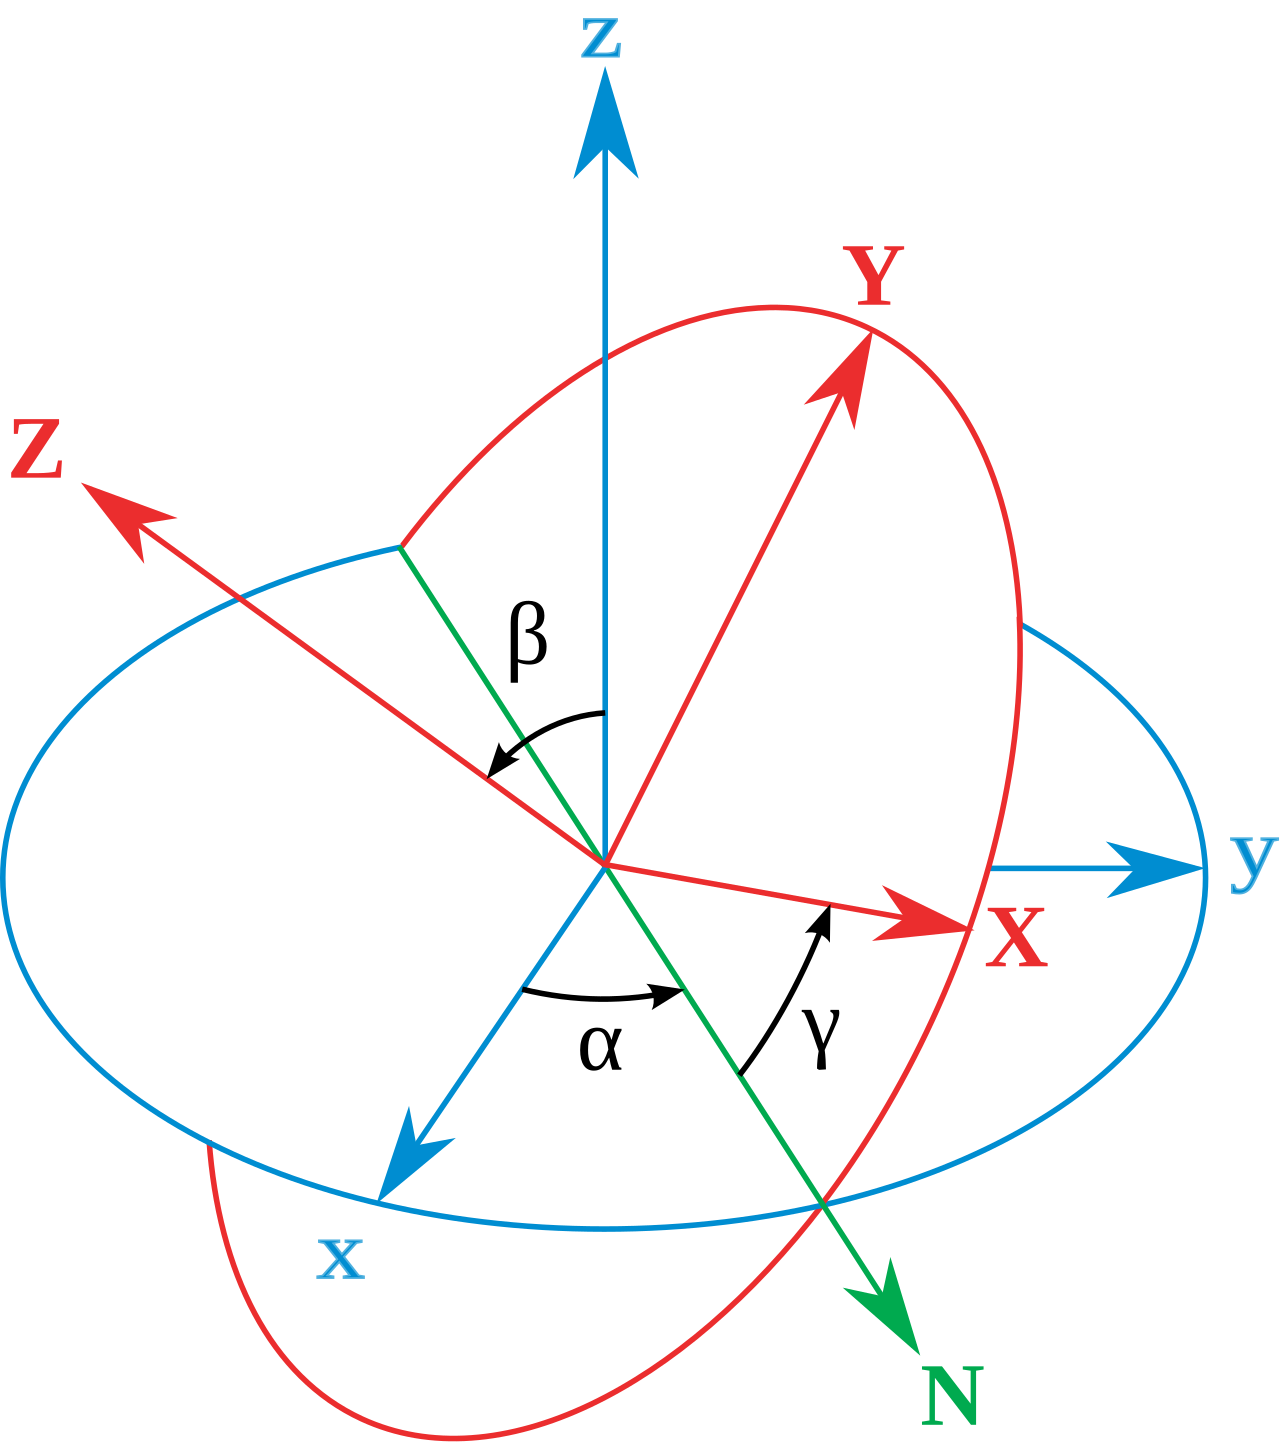
\includegraphics[width=0.6\textwidth, center]{Eulerangles.png}
   	 	\label{fig:eulero}
   	 	\caption{Gli angoli di Eulero: l'angolo $\alpha$ è l'angolo di precessione, l'angolo $\beta$ è l'angolo di nutazione, l'angolo $\gamma$ è quello di rotazione propria e l'asse $N$ è la retta dei nodi.}
   	 \end{figure}
   	 assumiamo che la trasformazione che stiamo considerando non sia l'identità, assumiamo inoltre che nessuno degli $e_i$ sia un autovalore della matrice (nel qual caso la descrizione di $R$ sarebbe molto facile, in quanto diventerebbe semplicemente una matrice di rotazione bidimensionale). Identifichiamo la \textit{retta dei nodi} (attenzione, questo \textbf{non è l'asse di rotazione}) con
   	 $$N\in \left\{e_3,E_3\right\}^\perp$$
   	 a questo punto definiamo i seguenti angoli:
   	 \begin{definition}[Angoli di Eulero]
   	 	Data una rotazione $R$ tridimensionale che non fissa nessun asse, denotata con $N$ la retta dei nodi 
   	 	$$N\in \left\{e_3,E_3\right\}$$
   	 	definiamo:
   	 	\begin{itemize}
   	 		\item  L'\textit{angolo di precessione} ($\alpha$ in figura) come l'angolo tra $N$ ed $e_1$.
   	 		\item  L'\textit{angolo di nutazione} ($\beta$ in figura) come l'angolo tra $e_3$ ed $E_3$.
   	 		\item  L'\textit{angolo di rotazione propria} ($\gamma$ in figura) come l'angolo tra $N$ ed $E_1$.
   	 	\end{itemize}
   	 \end{definition} 
   	 A questo punto enunciamo il teorema principale di questa sezione:
   	 \begin{theorem}[Angoli di Eulero per le rotazioni]
   	 	Ogni matrice ortogonale diretta tridimensionale $A\in \SO_3(\RR)$ può essere scritta come prodotto di tre rotazioni bidimensionali:
   	 	$$R=R_3R_2R_1$$
   	 	tali che:
   	 	\begin{itemize}
   	 		\item $R_1$ è una rotazione dell'angolo di precessione attorno all'asse $z$. 
   	 		\item $R_2$ è una rotazione dell'angolo di nutazione attorno all'asse $x$ (trasformato!).
   	 		\item $R_3$ è una rotazione dell'angolo di rotazione propria attorno all'asse $z$ (trasformato!).
   	 	\end{itemize}
   	 \end{theorem}
   	 \begin{proof}
   	 	Per definizione degli angoli di Eulero e delle rotazioni date sopra abbiamo che
   	 	\begin{gather*}
   	 		R_1:
   	 		\begin{cases}
   	 			R_1(e_3)=e_3 \\
   	 			R_1(e_1)=N
   	 		\end{cases} \\
   	 		R_2:\begin{cases}
   	 			R_2(N)=N \\
   	 			R_2(e_3)=E_3 
   	 		\end{cases} \\
   	 		R_3:\begin{cases}
   	 			R_3(E_3)=E_3 \\
   	 			R_3(N)= E_1
   	 		\end{cases}
   	 	\end{gather*}
   	 	Dunque notiamo che applicando una trasformazione alla volta abbiamo
   	 	$$R_3R_2R_1(e_1)=E_1$$
   	 	$$R_3R_2R_1(e_3)=E_3.$$
   	 	Ora dato che tutte le trasformazioni erano ortogonali dobbiamo avere che l'immagine di $R_3R_2R_1(e_2)$ deve essere di nuovo ortogonale sia ad $E_1$ che ad $E_3$ e deve avere norma $1$, quindi dev'essere
   	 	$$R_3R_2R_1(e_2)=\pm E_2$$
   	 	d'altra parte dato che tutte le trasformazioni avevano determinante $1$ dobbiamo per forza avere $R_3R_2R_1e_2=E_2$ e quindi abbiamo proprio che 
   	 	$$R=R_3R_2R_1$$
   	 	dato che le due trasformazioni sono uguali su una base ortonormale dello spazio.
   	 \end{proof}
   	 Notiamo che le tre matrici trovate si possono scrivere in modo molto conveniente come
   	 $$R=R_3R_2R_1=\begin{pmatrix}
   	 	A(\gamma) & 0 \\
   	 	0 & 1
   	 \end{pmatrix}
   	 \begin{pmatrix}
   	 	1 & 0 \\
   	 	0 & A(\beta)
   	 \end{pmatrix}
   	 \begin{pmatrix}
   	 	A(\alpha) & 0 \\
   	 	0 & 1
   	 \end{pmatrix}
   	 $$
   	 dove $A(\theta)$ è una rotazione in senso antiorario di angolo $\theta$, ovvero
   	 $$A(\theta):=
   	 \begin{pmatrix}
   	 	\cos\theta & -\sin \theta\\
   	 	\sin \theta & \cos \theta
   	 \end{pmatrix}.
   	 $$
   	 \subsection{Distanze e proiezioni}
   	 
   	 Finora abbiamo lavorato con spazi vettoriali Euclidei. Ora torniamo agli spazi affini, e dotiamoli di una struttura di prodotto scalare. 
   	 \begin{definition}[Spazio Euclideo]
   	 	Lo spazio affine $\AA_n(\RR)$ dotato di un prodotto scalare tra vettori si dice \textit{Spazio affine Euclideo}, o semplicemente \textit{spazio Euclideo} e si denota con $\mathbb{E}_n$.
   	 \end{definition}
   	 La prima cosa importante che possiamo fare è definire la distanza tra due punti in uno spazio Euclideo:
   	 \begin{definition}[Distanza tra punti]
   	 	Dati due punti $P,Q\in \mathbb{E}_n$ la loro distanza è la norma dell'unico vettore differenza, cioè
   	 	$$d\left(P,Q\right):=\abs{\abs{P-Q}}.$$
   	 \end{definition}
   	 Invece per i sottospazi possiamo definire
   	 \begin{definition}[Distanza tra sottospazi]
   	 	Dati due sottospazi $\mathbb{L},\mathbb{M}$ la \textit{distanza} tra di essi è definita come
   	 	$$d(\mathbb{L},\mathbb{M}):=\inf_{P\in \mathbb{L},Q\in \mathbb{M}}d(P,Q)$$
   	 \end{definition}
   	 \begin{theorem}[Pitagora]
   	 	Dati $n$ vettori $v_1,v_2,\dots,v_n$ ortogonali a due a due, abbiamo che 
   	 	$$\abs{\abs{\sum_{i=1}^{n}v_i}}^2=\sum_{i=1}^{n}\abs{\abs{v_i}}^2$$
   	 \end{theorem}
   	 \begin{proof}
   	 	Per induzione nel modo chiaro.
   	 \end{proof}
   	 \begin{lemma}[Unicità della proiezione]
   	 	Sia $\mathbb{L}\le \mathbb{E}_n$ un sottospazio affine e sia $V$ la sua giacitura. per ogni $P\in\mathbb{E}_n$ esiste un unico punto $Q\in\mathbb{L}$ tale che $P-Q\in V^\perp$.
   	 \end{lemma}
   	 \begin{proof}
   	 	Prendiamo un generico punto $R$ di $\mathbb{L}$. Allora dato che $V\oplus V^\perp=\RR^n$ possiamo scrivere 
   	 	$$P-R=v+w$$
   	 	dove $v\in V $ e $w\in  V^\perp$. D'altra parte dato che $R\in\mathbb{L}$ abbiamo che $R+v\in\mathbb{L}$, dunque se scegliamo
   	 	$$Q:=R+v$$ 
   	 	abbiamo
   	 	$$P-Q=P-(R+v)=v+w-v=w\in V^\perp$$
   	 	e dunque abbiamo che esiste sempre almeno un $Q$. Per l'unicità, supponiamo che vi siano due punti $Q_1,Q_2\in\mathbb{L}$ che soddisfano la proprietà, allora abbiamo che la loro differenza chiaramente apparterrà alla giacitura $V$ di $\mathbb{L}$, d'altra parte abbiamo
   	 	$$P-Q_1\in V^\perp$$
   	 	$$P-Q_2\in V^\perp$$
   	 	quindi anche la loro differenza sarà in $V^\perp$, ma allora $Q_1-Q_2\in V\cap V^\perp$, cioè $Q_1-Q_2=0$ cioè sono lo stesso punto.
   	 \end{proof}
   	 
   	 \begin{lemma}[Distanza Spazio-Punto]
   	 	Sia $\LL< \mathbb{E}_n$, e $P$ un punto, allora abbiamo che 
   	 	$$d(P,\mathbb{L}):=d\left(P,\pi_\mathbb{L}^\perp (P)\right)$$
   	 	cioè la proiezione ortogonale del punto $P$ è il punto che minimizza la distanza da $\LL$.
   	 \end{lemma}
   	 \begin{proof}
   	 	Prima di tutto dal fatto che $\pi_\LL^\perp(P)\in \LL$ segue che 
   	 	$$d(P,\LL):=\inf_{Q\in\LL}d(P,Q)\le d\left(P,\pi_\LL^\perp(P)\right)$$
   	 	a questo punto per ogni $Q\in \LL$ decomponiamo la differenza in una parte perpendicolare e una parte parallela, cioè abbiamo 
   	 	$$P-Q=v+w$$
   	 	per $v\in V$ (la giacitura di $\LL$) e $w\in V^\perp$. Allora per il teorema di Pitagora abbiamo che 
   	 	$$d(P,Q)^2:=\abs{\abs{v+w}}^2=\abs{\abs{v}}^2+\abs{\abs{w}}^2$$
   	 	d'altra parte per definizione di proiezione abbiamo che 
   	 	$$\pi_\LL^\perp(P)=\pi_\LL^\perp(Q+(P-Q))=\pi_\LL^\perp(Q+v+w)=Q+v=P-w$$
   	 	da cui abbiamo che 
   	 	$$d\left(P,\pi_\LL^\perp(P)\right)^2=\abs{\abs{w}}^2$$
   	 	cioè abbiamo dimostrato che
   	 	$$d(P,Q)=\abs{\abs{v}}^2+\abs{\abs{w}}^2\ge \abs{\abs{w}}^2=d\left(P,\pi_\LL^\perp(P)\right) $$
   	 	che conclude la dimostrazione.
   	 \end{proof}
   	 Abbiamo dunque dimostrato che nel caso particolare della distanza spazio-punto, la distanza (che è un inf per definizione), in realtà è un minimo, cioè esiste una coppia di punti che realizza la distanza minima. Vogliamo generalizzare questo risultato a coppie di spazi arbitrari:
   	 \begin{lemma}[Distanza Spazio-Spazio]
   	 	Siano $\LL$ e $\mathbb{M}$ due sottospazi affini di $\mathbb{E}_n$. Prendiamo i punti $P\in \LL$ e $Q\in\mathbb{M}$ e consideriamo $V_1,V_2$ le giaciture, allora se definiamo
   	 	$$W=\left(V_1+V_2\right)^\perp$$ 
   	 	allora abbiamo
   	 	$$d\left(\LL,\mathbb{M}\right)=\abs{\abs{\pi_W^\perp\left(P-Q\right)}}.$$
   	 \end{lemma}
   	 \begin{proof}
   	 	Possiamo decomporre (in modo non necessariamente unico) il vettore $P-Q$ come
   	 	$$P-Q=v_1+v_2+w$$
   	 	dove $v_1\in V_1,v_2\in V_2$ e $w\in W$. In particolare abbiamo che $w$ è proprio la proiezione ortogonale di $P-Q$ su $W$ che compare nella tesi. A questo punto allora notiamo che i punti $P-v_1$ e $Q+v_2 $ appartengono sempre rispettivamente agli spazi $\mathbb{L}$ e $\mathbb{M}$, cioè per il fatto che la distanza è l'inf delle coppie di distanze tra punti appartenenti ai due sottospazi abbiamo
   	 	$$d\left(\mathbb{L},\mathbb{M}\right)\le d\left(P-v_1,Q+v_2\right)=\abs{\abs{w}}$$ 
   	 	ora dato che $\abs{\abs{w}}$ è proprio la quantità che appare nella tesi al RHS ci basterebbe dimostrare che 
   	 	$$d\left(\mathbb{L},\mathbb{M}\right)\ge \abs{\abs{w}}$$
   	 	per avere la tesi. D'altra parte se prendiamo due generici punti $R,S$ rispettivamente in $\mathbb{L},\mathbb{M}$ possiamo scriverli in funzione di $P$ e $Q$ come
   	 	$$R=P+v_3$$
   	 	$$S=Q+v_4$$
   	 	e quindi la distanza tra di loro sarà
   	 	$$d\left(R,S\right)^2=\abs{\abs{R-S}}^2=\abs{\abs{P-Q+v_3-v_4}}^2=\abs{\abs{v_1+v_2+v_3-v_4+w}}^2=\abs{\abs{v_1+v_2+v_3-v_4}}^2+\abs{\abs{w}}^2$$
   	 	da cui la tesi segue, perchè abbiamo dimostrato che per ogni coppia di punti la distanza è 
   	 	$$d(R,S)=\dots =\abs{\abs{v_1+v_2+v_3-v_4}}^2+\abs{\abs{w}}^2\ge \abs{\abs{w}}^2$$
   	 	e quindi in particolare anche l'inf sarà $\ge \abs{\abs{w}}$, dunque la tesi.
   	 \end{proof}
   	 Ora vogliamo cercare un modo per calcolare esplicitamente le distanze che abbiamo trovato. La formula seguente è estremamente potente, e ci fa capire quanto sia comodo lavorare con spazi che hanno dimensione $n-1$:
   	 \begin{lemma}[Formula esplicita della distanza Punto-Spazio]
   	 	Prendiamo un punto $P\in\mathbb{E}_n$ e un iperpiano $\mathbb{H}$ (cioè un sottospazio di dimensione $n-1$) parametrizzato come
   	 	$$\mathbb{H}=\left\{\mathbf{x}\in\mathbb{E}_n:a_1x_1+a_2x_2+\dots+a_nx_n+b=0\right\}$$
   	 	per certi coefficienti $a_1,a_2,\dots,a_n,b\in\RR$. Allora abbiamo che 
   	 	$$d\left(P,\mathbb{H}\right)=\frac{\abs{a_1\bar{x}_1+a_2\bar{x}_2+\dots+a_n\bar{x}_n+b}}{\sqrt{a_1^2+a_2^2+\dots+a_n^2}}$$
   	 	dove gli $\bar{x}_i$ sono le coordinate del punto $P$ nel sistema di riferimento canonico.
   	 \end{lemma}
   	 \begin{proof}
   	 	L'idea chiave è che rappresentare un iperpiano è molto facile se ci si rende conto che il complementare della sua giacitura è un sottospazio vettoriale di dimensione $1$, quindi possiamo scrivere $\mathbb{H}$ come
   	 	$$\mathbb{H}=Q+\left(v\right)^\perp$$
   	 	dove $v$ è il vettore di componenti $(a_1,a_2,\dots,a_n)$. Allora possiamo scrivere la distanza utilizzando il lemma precedente:
   	 	$$d\left(P,\mathbb{H}\right)=\abs{\abs{\pi_W^\perp\left(P-Q\right)}}$$
   	 	ma notiamo che in questo caso abbiamo proprio che $$W=\left(v^\perp\right)^\perp=\langle v \rangle$$
   	 	da cui abbiamo, grazie al fatto che ha dimensione $1$, che la formula della proiezione si semplifica a 
   	 	$$\pi_W^\perp\left(P-Q\right)=\frac{\langle P-Q,v\rangle}{\langle v,v\rangle}v$$
   	 	d'altra parte se $Q$ ha coordinate $y_i$ la norma di quella proiezione si riscrive come
   	 	$$\abs{\abs{\frac{\langle P-Q,v\rangle}{\langle v,v\rangle}v}}^2=\frac{\left[a_1\left(\bar{x}_1-y_1\right)+a_2\left(\bar{x}_2-y_2\right)+\dots+a_n\left(\bar{x}_n-y_n\right)\right]^2}{a^2_1+a_2^2+\dots+a_n^2}$$
   	 	da cui osservando che
   	 	$$a_1y_1+\dots+a_ny_n=-b$$
   	 	dato che deve soddisfare l'equazione di $\mathbb{H}$, abbiamo proprio 
   	 	$$d(P,\mathbb{H})^2=\frac{\left[a_1\bar{x}_1+a_2\bar{x}_2+\dots+a_n\bar{x}_n+b\right]^2}{a^2_1+a_2^2+\dots+a_n^2}$$
   	 	che prendendo le radici è esattamente la tesi.
   	 \end{proof}
   	 
   	 \subsection{Similitudini e Rigidità}
   	 
   	 Abbiamo visto le trasformazioni affini e le mappe lineari conformi (e/o le isometrie). Mettendo insieme le due cose otteniamo le cosiddette \textit{rigidità}. In questa sezione ci interesseremo a trasformazioni affini $T:\mathbb{E}_n\to\mathbb{E}_n$ che siano endomorfismi dello spazio affine euclideo, e quindi dove non specificato altrimenti assumeremo che le trasformazioni che consideriamo siano tutte endomorfismi di $\mathbb{E}_n$. Diamo la seguente definizione:
   	 \begin{definition}[Similitudini e rigidità]
   	 	Una trasformazione affine $F$ è una \textit{similitudine} se la sua applicazione soggiacente $\varphi$ è conforme. In particolare $F$ è una \textit{rigidità} se la sua applicazione soggiacente è un'isometria.
   	 \end{definition}
   	 \begin{definition}[Similitudini e rigidità dirette e inverse]
   	 	Se $F$ è una similitudine o una rigidità si dice \textit{diretta} se ha determinante positivo, e \textit{inversa} se ha determinante negativo.
   	 \end{definition}
   	 \begin{definition}[Similitudini centrate e asse]
   	 	Una similitudine $F$ si dice \textit{centrata} se esiste un almeno un punto $P$ tale che $F(P)=P$. Chiamiamo \textit{asse} di $F$ l'insieme dei punti $P$ tali che $F(P)=P$, ovvero l'autospazio di autovalore $1$.
   	 \end{definition}
   	 \begin{lemma}[Decomposizione Kernel-Immagine]
   	 	Sia $\lambda$ un autovalore di $A\in K_{n\times n}$ tale che la sua molteplicità geometrica è uguale a quella algebrica, allora
   	 	$$K^n=\ker{A-\lambda I}\oplus \Immagine{A-\lambda I}.$$
   	 \end{lemma}
   	 \begin{proof}
   	 	Dal teorema rango-nullità sappiamo che le dimensioni sono quelle giuste, non rimane che dimostrare che
   	 	$$\ker{A-\lambda I}\cap \Immagine{A-\lambda I}=\left\{0\right\}$$
   	 	d'altra parte prendiamo un 
   	 	\begin{gather*}
   	 		v\in \Immagine{A-\lambda I } \\
   	 		v\in \ker{A-\lambda I}
   	 	\end{gather*}
   	 	per la prima condizione esiste un $w$ tale che
   	 	$$\left(A-\lambda I\right)w=v$$
   	 	e per la seconda
   	 	$$\left(A-\lambda I\right)^2w=0$$
   	 	ma allora se $v\ne 0$ abbiamo che $A$ ristretta allo spazio $\langle \left\{v,w\right\} \rangle$ è un blocco di Jordan, in particolare è proprio
   	 	$$\begin{pmatrix}
   	 		\lambda & 1 \\
   	 		0 & \lambda
   	 	\end{pmatrix}$$
   	 	ma d'altra parte per l'ipotesi du $\lambda$ dovremmo avere che i blocchi di Jordan con autovalore $\lambda$ siano tutti di dimensione al più $1$, quindi questo è assurdo per unicità della jordanizzazione.
   	 \end{proof}
   	 Il lemma precedente ci serviva per la seguente proposizione, che ci servirà a classificare le rigidità:
   	 \begin{proposition}[Rigidità che agiscono come traslazioni]
   	 	Sia $F:\mathbb{E}_n\to\mathbb{E}_n$ una rigidità che rispetto ad un sdr ortonormale ha matrice
   	 	$$
   	 	\left(
   	 	\begin{array}{c|c}
   	 		1 & 0 \\
   	 		\hline 
   	 		b & A
   	 	\end{array}
   	 	\right)
   	 	$$
   	 	allora se le molteplicità algebrica e geometrica dell'autovalore $1$ (della matrice $A$) sono uguali abbiamo che esiste un $P$ tale che 
   	 	$$F(P)-P\in V_1(A)$$
   	 	l'autospazio di autovalore $1$ di $A$. Inoltre per ogni $Q$ tale che $F(P)-P\in V_1(A)$ esiste un unico $v\in V_1(A)$ tale che
   	 	$$F(Q)=Q+v$$
   	 	ovvero $F$ agisce come una traslazione su tutti i punti negli spazi con giacitura l'autospazio di autovalore $1$ di $A$.
   	 \end{proposition}
   	 \begin{proof}
   	 	Per dimostrare l'esistenza di almeno un punto tale che $F(P)-P$ è nell'asse di $A$ prendiamo un punto $P_0$ e consideriamo il vettore
   	 	$$F(P_0)-P_0=v$$
   	 	per il lemma precedente lo possiamo decomporre univocamente in due vettori 
   	 	$$v=a+b$$
   	 	tali che $a\in V_1(A)$ e $b=(A-I)c$ per qualche $c$. Il punto candidato dunque è
   	 	$P:=P_0-c$:
   	 	$$F(P)-P=F(P_0)-Ac-P_0+c=F(P_0)-P_0-(A-I)c=v-b=a\in V_1(A)$$
   	 	e quindi abbiamo proprio quello che volevamo. Per dimostrare che tale vettore è unico consideriamo 
   	 	\begin{gather*}
   	 		F(P)-P=v\in V_1(A) \\
   	 		F(Q)-Q=w\in V_1(A)
   	 	\end{gather*}
   	 	allora sottraendo membro a membro abbiamo
   	 	$$F(P)-F(Q)-(P-Q)=v-w$$
   	 	ovvero 
   	 	\begin{gather*}
   	 		A(P-Q)-(P-Q)=v-w \\
   	 		(A-I)(P-Q)=v-w
   	 	\end{gather*}
   	 	il che implica 
   	 	\begin{gather*}
   	 		v-w\in \Immagine{A-I}
   	 	\end{gather*}
   	 	ma d'altra parte per chiusura di $V_1(A)$ abbiamo $v-w\in \ker{A-I}$ il che vuol dire proprio che $v-w=0$, che era la tesi.
   	 \end{proof}
   	 Come corollario otteniamo il seguente potente risultato
   	 \begin{corollary}[Punti fissi di omotetie]
   	 	Sia $F:\mathbb{E}_n\to \mathbb{E}_n$ una similitudine che non è una rigidità, allora ha un punto fisso.
   	 \end{corollary}
   	 \begin{proof}
   	 	Se $F$ non è una rigidità vuol dire che esiste un sistema di riferimento in cui la sua matrice si scrive come
   	 	$$
   	 	\left(
   	 	\begin{array}{c|c}
   	 		1 & 0 \\
   	 		\hline
   	 		b & A
   	 	\end{array}
   	 	\right)
   	 	$$
   	 	e $A$ è conforme con indice di conformità diverso da $1$. Dato che tutti gli autovalori di una mappa conforme hanno modulo l'indice di conformità, e abbiamo che questo è $\ne 1$ l'autospazio di autovalore $1$ di $A$ sarà vuoto $\left(0\right)$, ovvero per il lemma precedente esisterà un $P$ tale che
   	 	$$F(P)-P\in \left\{0\right\}$$
   	 	cioè $P$ sarà un punto fisso di $F$.
   	 \end{proof}
   	 A questo punto possiamo classificare tutte le rigidità in dimensione $2$ e $3$. Per farlo partiamo dalla classificazione delle matrici ortogonali: dal teorema di classificazione segue che le matrici ortogonali $2\times 2$ possono essere solo
   	 $$
   	 \begin{pmatrix}
   	 	1 & 0 \\
   	 	0 & 1
   	 \end{pmatrix},
   	 \begin{pmatrix}
   	 	1 & 0 \\
   	 	0 & -1
   	 \end{pmatrix},
   	 \begin{pmatrix}
   	 	\cos\theta & -\sin\theta \\
   	 	\sin\theta & \cos\theta
   	 \end{pmatrix}
   	 $$
   	 dunque come conseguenza otteniamo il teorema di classificazione delle rigidità:
   	 \begin{theorem}[Classificazione delle rigidità 2D]
   	 	Se $F:\mathbb{E}_2\to\mathbb{E}_2$ è una rigidità allora ci sono solo $5$ possibilità:
   	 	\begin{enumerate}
   	 		\item $F$ è l'identità.
   	 		\item $F$ è una traslazione.
   	 		\item $F$ è una riflessione in una retta fissa.
   	 		\item $F$ è una rotazione attorno ad un punto fisso.
   	 		\item $F$ è una \textit{glissoriflessione}, cioè una riflessione seguita da una traslazione lungo l'asse di riflessione.
   	 	\end{enumerate}
   	 \end{theorem}
   	 \begin{proof}
   	 	Per quanto detto sopra sulle matrici ortogonali la soggiacente può avere solo $3$ forme:
   	 	\begin{description}
   	 		\item[Identità:] Per il lemma precedente se la soggiacente è l'identità vuol dire che il suo autospazio di $1$ sarà tutto lo spazio, il che vuol dire che $F$ agirà come una traslazione su tutto lo spazio. Questo ci porta ai casi $2$ e $1$ (se è la traslazione di vettore nullo).
   	 		\item[Riflessione:] Di nuovo per il lemma precedente abbiamo che l'autospazio di $1$ (che ha molteplicità geometrica uguale a quella algebrica) ha dimensione $1$, dunque possiamo scrivere $F$ come
   	 		$$
   	 		\left(
   	 		\begin{array}{c|cc}
   	 			1 & 0 & 0 \\
   	 			\hline
   	 			a_1 & -1 & 0 \\
   	 			0 & 0 & 1
   	 		\end{array}
   	 		\right)
   	 		$$ 
   	 		il che ci porta ai casi $3$ e $5$.
   	 		\item[Rotazione:] In questo caso l'autovalore di $1$ è banale, e quindi la trasformazione avrà almeno un punto fisso, rispetto al quale è una rotazione, che era il caso $4$.
   	 	\end{description} 
   	 	Dunque in ogni caso ci riconduciamo alla tesi, e abbiamo finito.
   	 \end{proof}
   	 Analogamente si può fare in dimensione $3$.
   	 \subsection{Angoli tra sottospazi euclidei}
   	 
   	 Prendiamo due $v,w$ vettori non nulli. Abbiamo già discusso cosa voglia dire parlare dell'"angolo" che c'è tra di essi, ovvero è è il minimo numero $\theta\in [0,2\pi]$ tale che
   	 $$\cos \theta=\frac{\abs{\abs{v}}\abs{\abs{w}}}{\langle v,w\rangle}.$$
   	 Prendiamo allora due rette incidenti $\LL$ ed $\mathbb{M}$ tali che
   	 $$\mathbb{L}=P+\langle v\rangle $$
   	 $$\mathbb{M}=Q+\langle w\rangle $$
   	 allora ci verrebbe da definire l'angolo tra queste due rette come, di nuovo
   	 $$\cos \theta=\frac{\abs{\abs{v}}\abs{\abs{w}}}{\langle v,w\rangle}$$
   	 il problema è che questa cosa dipende dal valore dei vettori $v,w$, infatti moltiplicandoli per uno scalare (cioè sostituendo $\lambda v,\mu w$) abbiamo
   	 $$\cos\theta=\frac{\abs{\abs{\lambda v}}\abs{\abs{\mu w}}}{\langle \lambda v,\mu w\rangle}=\frac{\abs{\lambda \mu} }{\lambda \mu}\frac{\abs{\abs{v}}\abs{\abs{w}}}{\langle v,w\rangle}$$
   	 che cambia solo di un segno. Questo giustifica la seguente definizione:
   	 \begin{definition}[Valore assoluto di un angolo fra rette]
   	 	Date due rette $\LL$ e $\mathbb{M}$ incidenti e con giaciture $\langle v\rangle$ e $\langle w \rangle$ definiamo il valore assoluto del coseno dell'angolo compreso tra di esse come
   	 	$$\abs{\cos \theta}=\frac{\abs{\abs{v}}\abs{\abs{w}}}{\langle v,w\rangle}.$$
   	 \end{definition}
   	 Questo discorso si può applicare facilmente anche agli iperpiani $n-1$ dimensionali, considerando i complementi ortogonali:
   	 \begin{definition}[Vettore normale ad un iperpiano $n-1$ dimensionale]
   	 	Dato un iperpiano $n-1$ dimensionale parametrizzato come
   	 	$$a_1x_1+\dots+a_nx_n+b=0$$
   	 	definiamo il suo \textit{vettore normale} come il vettore
   	 	$$\vec{n}:=\frac{1}{\sqrt{a_1^2+a_2^2+\dots+a_n^2}}
   	 	\begin{pmatrix}
   	 		a_1 \\
   	 		a_2 \\
   	 		\vdots \\
   	 		a_n
   	 	\end{pmatrix}$$
   	 	che chiaramente costituisce una base ortonormale del complemento ortogonale dell'iperpiano.
   	 \end{definition}
   	 \begin{definition}[Angolo tra iperpiani e rette]
   	 	Data una retta $P+\langle v\rangle$ e un iperpiano $\mathbb{L}$ di vettore normale $n$ l'angolo tra essi compresi è il numero 
   	 	$$\theta-\frac{\pi}{2}$$
   	 	dove $\theta$ è l'angolo \textit{tra la normale al piano e la retta}, cioè
   	 	$$\abs{\cos\theta}=\frac{\abs{\abs{v}}\abs{\abs{n}}}{\langle v,n\rangle}.$$
   	 \end{definition}
   	 
   	 
   	 \newpage
   	 
   	 \section{Geometria Proiettiva}
   	 In questo capitolo denotiamo con $e_0,e_1,\dots,e_n$ i vettori della base canonica di $K^{n+1}$. \\
   	 Sia $K$ un campo. Ricordiamo che $K^*$ è il gruppo delle unità di $K$, ovvero 
   	 $$K^*:=K\setminus\left\{0\right\}$$
   	 dato un intero $n$ vogliamo definire lo \textit{spazio proiettivo} $\mathbb{P}^n_K$ (sul campo $K$) come le direzioni di $K^{n+1}$. Questo corrisponde all'insieme di tutti i sottospazi vettoriali di dimensione $1$ di $K^{n+1}$. Dunque definiamo
   	 \begin{definition}[Proiettivizzazione e spazio proiettivo standard]
   	 	Sia $V$ un $K$-spazio vettoriale. Allora definiamo la \textit{proiettivizzazione} di $V$ lo spazio 
   	 	$$\PP(V):=\left\{U\le V:\dim U =1\right\}$$
   	 	e inoltre definiamo lo \textit{spazio proiettivo standard} come
   	 	$$\PP^n_K:=\PP(K^{n+1}).$$
   	 	\textbf{ATTENZIONE:} lo spazio proiettivo per come lo abbiamo definito non ha ancora una nozione ben definita di "somma tra elementi", infatti la somma di due spazi di dimensione $1$ è uno spazio di dimensione $2$ e così via. Dunque non dotiamo automaticamente lo spazio $\PP(V)$ di una struttura di spazio vettoriale, e di conseguenza per noi gli elementi di $\PP(V)$ saranno \textit{punti}.
   	 \end{definition}
   	 Notiamo prima di tutto che la proiettivizzazione di uno spazio è più piccola dello spazio stesso, infatti a ogni vettore possiamo associare il sottospazio generato da se stesso, in questo modo abbiamo la seguente mappa suriettiva
   	 \begin{align*}
   	 	\varphi:V &\to \PP(V) \\
   	 	v & \mapsto  \langle v \rangle 
   	 \end{align*}   	 
   	 che non è quasi mai iniettiva, in quanto se esiste uno scalare $\lambda$ diverso da $0$ e diverso da $1$ abbiamo che 
   	 $$\langle v \rangle=\langle \lambda v \rangle$$
   	 e quindi la mappa non è iniettiva. Un modo per renderla iniettiva tuttavia è quello di quozientare per un insieme opportuno, in particolare l'insieme per cui vogliamo quozientare è quello contenente tutti e soli gli scalari non nulli, ovvero $K^*$, quindi abbiamo costruito una biezione
   	 $$\varphi: \faktor{V}{K^*}\to \PP(V)$$
   	 questo motiva la seguente definizione:
   	 \begin{definition}[Coordinate omogenee]
   	 	Denotiamo con 
   	 	$$(x_0:x_1:x_2:\dots:x_n)$$
   	 	la classe di equivalenza del punto $P\in K^{n+1}$ di coordinate $x_0,x_1,\dots,x_n$ nella base canonica. Queste sono le cosiddette \textit{coordinate omogenee} del punto $P'\in \PP(K^{n+1})$.
   	 \end{definition}
   	 Notiamo che tutti gli spazi proiettivi si prestano ad essere riscritti come
   	 \begin{lemma}[Ricoprimenti affini di spazi proiettivi]
   	 	Per ogni campo $K$ e intero $n$ lo spazio proiettivo standard si può riscrivere come
   	 	$$\PP^n=\AA^{n}\cup \AA^{n-1}\cup \AA^{n-2}\cup\dots\cup \AA^0$$
   	 	dove gli $\AA^i$ sono spazi affini standard di dimensione $i$ (ricordiamo che stiamo lavorando con punti, quindi preferiamo denotare con $\AA^i$ l'insieme $K^i$).
   	 \end{lemma}
   	 \begin{proof}
   	 	Per ogni punto $P\in\PP^n$ ha senso chiedersi quale sia la prima coordinata non nulla, se questa è al posto $0\le i\le n$ possiamo dividere le sue coordinate omogenee tutte per $x_i$ e ottenere una cosa del tipo
   	 	$$P=\left(0:\dots:0:x_i:x_{i+1}:\dots:x_n\right)=\left(0:0:\dots:0:1:\frac{x_{i+1}}{x_i}:\frac{x_{i+2}}{x_i}:\dots:\frac{x_n}{x_i}\right)$$
   	 	e notiamo che questo è a meno di omomorfismi una copia di $K^{n-i-1}$. Dunque ogni vettore appartiene sempre ad uno degli spazi $\AA^{n-i}$ da cui segue la tesi.
   	 \end{proof}
   	 Da quanto detto finora dunque è chiara la motivazione della seguente definizione:
   	 \begin{definition}[Dimensione di uno spazio proiettivo]
   	 	Dato uno spazio vettoriale $W$ definiamo la \textit{dimensione} della sua proiettivizzazione come 
   	 	$$\dim\PP(W):=\dim W-1.$$
   	 	In particolare abbiamo che la dimensione di $\eset$ è $-1$. 
   	 \end{definition}
   	 Inoltre definiamo
   	 \begin{definition}[Sottospazio proiettivo]
   	 	Dato $\PP(V)$ un suo \textit{sottospazio proiettivo} è un sottoinsieme $J$ tale che esiste un $W\le V$ che soddisfa
   	 	$$\PP(W)=J.$$
   	 	In particolare denotiamo con $S(V)$ l'insieme dei sottospazi proiettivi di $V$.
   	 \end{definition}
   	 \begin{remark}
   	 	Per come abbiamo dato le definizioni, un punto è un sottospazio proiettivo, ovvero se $W$ è un sottospazio vettoriale di dimensione $1$ allora $\PP(W)$ è un sottospazio proiettivo.
   	 \end{remark}
   	 \subsection{Omogeneizzare e deomogeneizzare}
   	 \'E chiaro che i sottospazi proiettivi di $\PP(V)$ siano in corrispondenza biunivoca con i sottospazi vettoriali di $V$. Tuttavia abbiamo detto che $\PP$ in generale è un insieme di \textit{punti}, quindi vorremmo trovare una corrispondenza biunivoca naturale con sottospazi affini, non con sottospazi vettoriali.
   	 \begin{remark}
   	 	Dato un sottospazio $W< K^{n+1}$ e $v_0,v_1,\dots,v_k$ una sua base possiamo scrivere ogni vettore di componenti $X_i$ in $W$ come
   	 	$$\begin{pmatrix}
   	 		X_0 \\
   	 		X_1 \\
   	 		\vdots \\
   	 		X_n
   	 	\end{pmatrix}
   	 	=
   	 	t_0v_0+\dots+t_kv_k
   	 	$$
   	 	osserviamo allora che $n> k$, e quindi sicuramente il sistema sarà in qualche modo sottodeterminato. Possiamo effettivamente risolvere con l'eliminazione di Gauss il sistema, trovando $n-k$ equazioni lineari in termini di $X_0,X_1,\dots,X_n$ uguali a $0$, ovvero troviamo una matrice $A\in K_{(n-k)\times (n+1)}$. Tale che 
   	 	$$AX=0.$$
   	 	La forma iniziale da cui siamo partiti di solito si dice sistema di \textit{equazioni parametriche} di $W$, mentre quella a cui siamo arrivati si chiama \textit{sistema di equazioni omogenee}.
   	 \end{remark}
   	 In effetti notiamo che ogni sottospazio di $\PP^n$ può essere facilmente messo in biezione (in modo da conservare la struttura, che vedremo sarà quella di reticolo) con un sottospazio di $\AA^n$. \\
   	 Il processo è la cosiddetta \textit{omogeneizzazione}, ovvero:
   	 \begin{description}
   	 	\item[Deomogeneizzazione:] Preso un sottospazio proiettivo $\PP(W)\le \PP(V)$ di equazioni omogenee lo possiamo deomogeneizzare ottenendo spazi affini in $\AA^n$ imponendo che una delle coordinate sia uguale a $1$. Se il sistema omogeneo è
   	 	$$A\begin{pmatrix}
   	 		X_0 \\
   	 		X_1 \\
   	 		\vdots \\
   	 		X_n
   	 	\end{pmatrix}=0$$
   	 	lo spazio $U_i\le \AA^n$ sarà quello che soddisfa il sistema di equazioni:
   	 	$$A\begin{pmatrix}
   	 		X_0 \\
   	 		X_1 \\
   	 		\vdots \\
   	 		X_{i-1} \\
   	 		1 \\
   	 		X_{i+1} \\
   	 		\vdots \\
   	 		X_n
   	 	\end{pmatrix}=0$$
   	 	ovvero, riscrivendolo in una maniera che siamo più abituati a vedere
   	 	$$A_i\begin{pmatrix}
   	 		X_0 \\
   	 		X_1 \\
   	 		\vdots \\
   	 		X_{i-1} \\
   	 		X_{i+1} \\
   	 		\vdots \\
   	 		X_n
   	 	\end{pmatrix}=-\begin{pmatrix}
   	 	a_{1i} \\
   	 	a_{2i} \\
   	 	a_{3i} \\
   	 	\vdots \\
   	 	a_{n-k-2,i} \\
   	 	a_{n-k-1,i}\\
   	 	a_{n-k,i}
   	 	\end{pmatrix}$$
   	 	dove $A_i$ è la matrice $(n-k) \times n $ ottenuta cancellando dalla matrice $A$ la colonna $i$ (e quindi appunto gli $a_{ij}$ sono i coefficienti della colonna $i$).
   	 	\item[Omogeneizzazione:] Viceversa, prendiamo un sottospazio affine $\LL$ di equazioni
   	 	$$AX=b$$
   	 	vogliamo ricondurci ad un sistema a $n+1$ incognite omogeneo. Per fare ciò applichiamo il procedimento sopra al contrario, cioè introduciamo una incognita $X_0$ e consideriamo tutte le incognite $X_i$ come se fossero state rinormalizzate rispetto a $X_0$, cioè il sistema diventa
   	 	$$
   	 	\begin{pmatrix}
   	 		a_{11} & a_{12} & \dots & a_{1n} \\
   	 		a_{21} & a_{22} & \dots & a_{2n} \\
   	 		\vdots & \vdots & \ddots & \vdots \\
   	 		a_{n-k,1} & a_{n-k,2} & \dots & a_{n-k,n}
   	 	\end{pmatrix}
   	 	\begin{pmatrix}
   	 		X_1/X_0 \\
   	 		X_2/X_0 \\
   	 		\vdots  \\
   	 		X_n/X_0
   	 	\end{pmatrix}=\begin{pmatrix}
   	 	b_1 \\
   	 	b_2 \\
   	 	\vdots \\
   	 	b_n
   	 	\end{pmatrix}
   	 	$$
   	 	che moltiplicando da entrambi i lati per $X_0$ e portando a sinistra diventa
   	 	$$(-b\mid A)X'=0$$
   	 	dove $X'$ è il vettore $X_0,X_1,\dots,X_n$. Dunque il sistema trovato è il sistema omogeneo di un certo spazio proiettivo $\PP(W)$ e abbiamo finito. \\ In realtà c'è una grossa differenza tra i due spazi, ovvero il sistema omogeneo $$(-b\mid A)X'=0$$
   	 	ha sempre soluzione, mentre 
   	 	$$AX=b$$
   	 	ha soluzione solo quando (per Rouchè-Capelli) $\rank{A}=\rank{A\mid b}$. In effetti notiamo che se effettivamente il sistema affine ha soluzione allora le dimensioni sono
   	 	$$\dim W=n+1-\rank{-b\mid A}=n+1-\rank{b\mid A}$$
   	 	$$\dim \LL=n-\rank{A}=n-\rank{b\mid A}$$
   	 	e quindi per prima cosa capiamo perchè abbiamo dato quella definizione di dimensione di uno spazio proiettivo, infatti abbiamo
   	 	$$\dim\PP(W)=\dim W-1=\dim\LL$$
   	 	e per seconda notiamo che effettivamente per $X_0=1$ abbiamo le soluzioni del sistema affine, e quindi i punti di $\LL$ (insomma stiamo intersecando l'iperpiano $X_0=1$ con il sottospazio vettoriale $W$). \\
   	 	\begin{figure}[h]
   	 		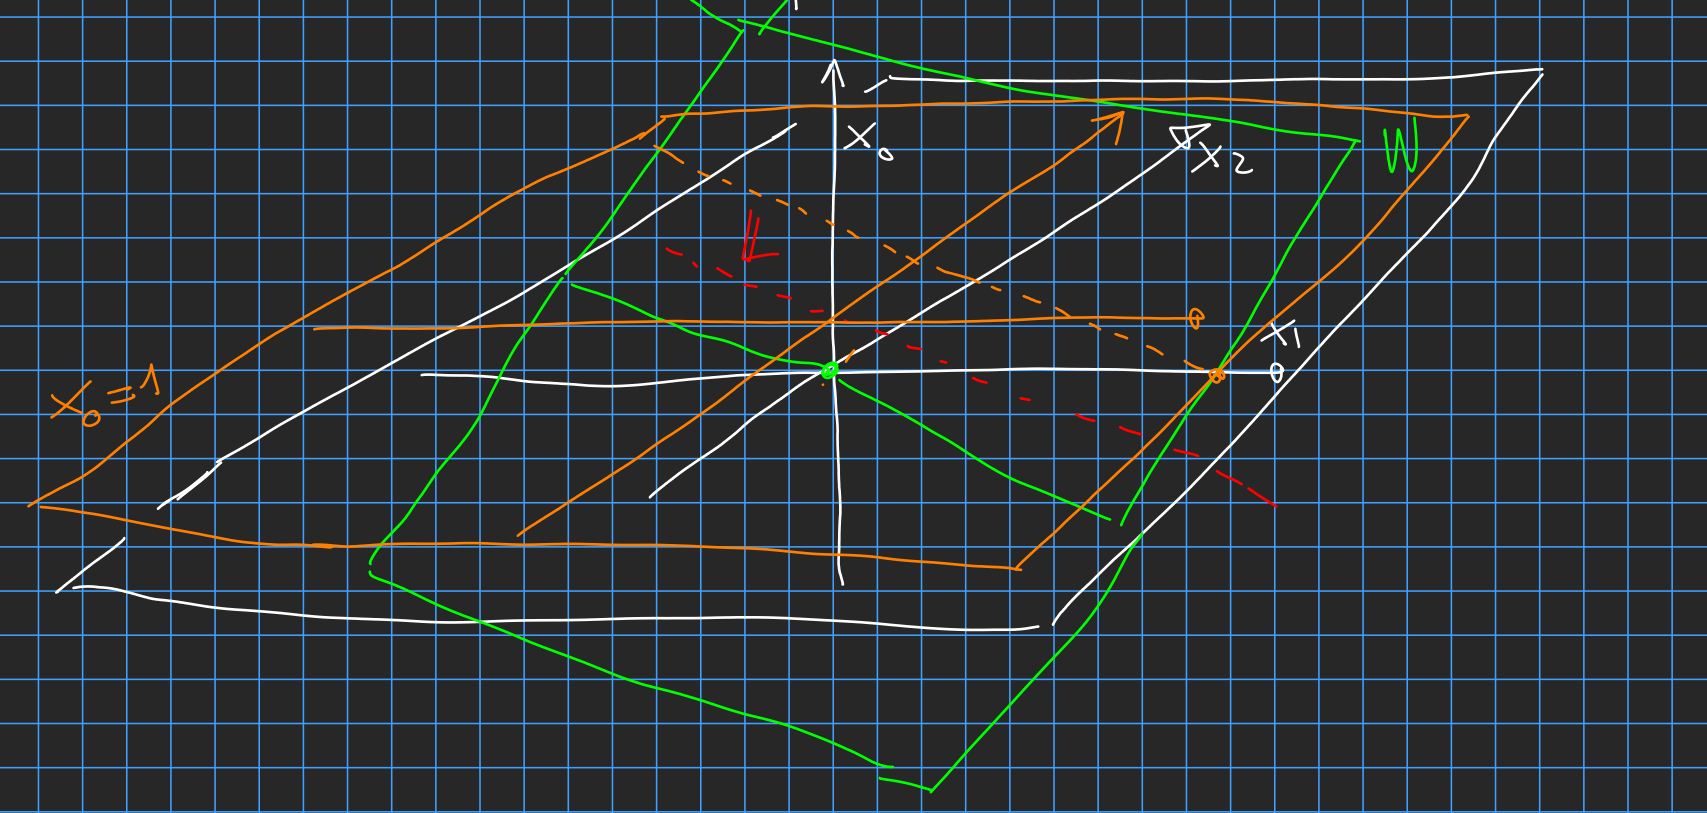
\includegraphics[width=1\textwidth, center]{spazi_proiettivi.png}
   	 		\caption{Una rappresentazione (molto amatoriale) del caso $n=2$ della deomogeneizzazione dello spazio $\PP(W)$.}
   	 		\label{fig:figure1}
   	 	\end{figure}
   	 	\begin{figure}[h]
   	 		\begin{center}
   	 			\begin{tikzpicture}
   	 				\begin{axis}[
   	 					view={115}{25},
   	 					width=13cm,
   	 					height=9cm,
   	 					xmin=-2.5, xmax=2.5,
   	 					ymin=-2.5, ymax=2.5,
   	 					zmin=-1.5, zmax=2,
   	 					axis lines=center,
   	 					axis line style={black, thick},
   	 					xlabel={$x$},
   	 					ylabel={$y$},
   	 					zlabel={$z$},
   	 					xtick=\empty,
   	 					ytick=\empty,
   	 					ztick=\empty,
   	 					]
   	 					
   	 					% ======================
   	 					% Piano bianco (bordo)
   	 					% ======================
   	 					\addplot3[black, thick]
   	 					coordinates {
   	 						(-2,-2,0) (2,-2,0) (2,2,0) (-2,2,0) (-2,-2,0)
   	 					};
   	 					
   	 					\node at (axis cs:2,2,0) {$\pi_0$};
   	 					
   	 					% ======================
   	 					% Piano arancione (bordo)
   	 					% ======================
   	 					\addplot3[orange, thick]
   	 					coordinates {
   	 						(-2,-2,1) (2,-2,1) (2,2,1) (-2,2,1) (-2,-2,1)
   	 					};
   	 					
   	 					\node[orange] at (axis cs:2,2,1) {$\pi_1$};
   	 					
   	 					% ======================
   	 					% Piano verde (bordo)
   	 					% ======================
   	 					\addplot3[green!50!black, thick]
   	 					coordinates {
   	 						(-2,0,2) (0,2,-2) (2,0,-2) (0,-2,2) (-2,0,2)
   	 					};
   	 					
   	 					\node[green!50!black] at (axis cs:-2,2,0) {$\pi$};
   	 					
   	 					% ======================
   	 					% Intersezione con piano bianco
   	 					% ======================
   	 					\addplot3[
   	 					very thick,
   	 					green!60!black,
   	 					domain=-2:2
   	 					]
   	 					({x},{-x},{0});
   	 					
   	 					\node[green!60!black] at (axis cs:1,-1,0) {$r$};
   	 					
   	 					% ======================
   	 					% Intersezione con piano arancione
   	 					% ======================
   	 					\addplot3[
   	 					very thick,
   	 					orange,
   	 					domain=-2:2
   	 					]
   	 					({x},{-x-1},{1});
   	 					
   	 					\node[orange] at (axis cs:1,-2,1) {$r'$};
   	 					
   	 					% ======================
   	 					% Proiezione (retta L)
   	 					% ======================
   	 					\addplot3[
   	 					red,
   	 					dashed,
   	 					very thick,
   	 					domain=-2:2
   	 					]
   	 					({x},{-x-1},{0});
   	 					
   	 					\node[red] at (axis cs:1,-2,0) {$L$};
   	 					
   	 				\end{axis}
   	 			\end{tikzpicture}
   	 		\end{center}
   	 		\caption{Una rappresentazione in pgfplots AI-assisted della deomogeneizzazione. Il lettore giudichi quale delle due figure è più chiara.}
   	 		\label{fig:figure2}
   	 	\end{figure}
   	 	D'altra parte se il sistema non ha soluzione vuol dire che intersecare $W$ con $X_0=k$ per qualunque $k\ne 0$ ci dà l'insieme vuoto, insomma abbiamo che $W$ è contenuto nel sottospazio di $K^{n+1}$ avente $X_0=0$ isomorfo a $K^n$. D'altra parte ci viene molta voglia di "estendere" $\AA^n$ in modo che anche questi spazi $\PP(W)$ "patologici" abbiano una controparte in $\AA^n$. Questa è proprio la nozione di \textit{punti all'infinito}, che vedremo meglio poi.
   	 \end{description}
   	 E quindi possiamo definire:
   	 \begin{definition}[Chiusura Proiettiva]
   	 	Dato uno spazio affine $\AA^n$ e una omogeneizzazione della coordinata $i$-esima di $\PP^n$:
   	 	$$\varphi_i:S(\AA^n)\to S(\PP^n)$$
   	 	per ogni $\LL\le \AA^n$ definiamo la sua \textit{chiusura proiettiva}, e la denotiamo con $\overline{\LL}$, il più piccolo sottospazio di $\PP^n$ contenente $\varphi_i(\LL)$ (ovvero, il risultato del processo di omogeneizzazione discusso sopra). Vedremo poi che la chiusura proiettiva consiste dei punti di $\LL$ a cui sono stati aggiunti i punti \textit{all'infinito}.
   	 \end{definition}
   	 \subsection{Modelli di $\PP^n$}
   	 Vogliamo trovare un modello che soddisfi la definizione di $\PP^n$. Consideriamo la sfera di dimensione $k$ tale che
   	 $$\mathbb{S}^{n+1}:=\left\{v\in \RR^{n+1}:\abs{\abs{v}}=1\right\}$$
   	 notiamo subito che esiste una biezione naturale tra punti di $\mathbb{S}^k$ e $\PP^k$, infatti possiamo costruire una mappa 
   	 \begin{align*}
   	 	\varphi:\mathbb{S}^k\to &\PP^k \\
   	 	v\mapsto & \langle v \rangle
   	 \end{align*}
   	 che chiaramente copre ogni elemento di $\PP^{n+1}$, perché esiste una base ortonormale per ogni sottospazio di dimensione $1$ e $\mathbb{S}^k$ è per definizione l'insieme che contiene tutte queste basi ortonormali. D'altra parte purtroppo questa mappa non è iniettiva, e per renderla biettiva dobbiamo quozientare per $\left\{-1,1\right\}$, perchè come è chiaro 
   	 $$v\mapsto \langle v\rangle$$
   	 $$-v\mapsto \langle v \rangle$$
   	 dunque abbiamo
   	 \begin{example}[Modello del piano proiettivo reale]
   	 	Un modello del piano proiettivo reale è
   	 	$$\faktor{\mathbb{S}^k}{\left\{-1,1\right\}}\simeq \PP^n.$$
   	 \end{example}
   	 Porta ad una costruzione ancora più naturale considerare la sfera \textit{complessa} $2n+1$-dimensionale immersa nello spazio hermitiano $\CC^{n+1}$ di dimensione $2n+2$:
   	 $$\mathbb{S}^{2n+1}:=\left\{v\in \CC^{n+1}:\abs{\abs{v}}=1\right\}$$
   	 la norma hermitiana ricordiamo essere definita esattamente come quella euclidea, e quindi anche qui abbiamo un'immersione molto naturale di $\PP^n_\CC$ in $\mathbb{S}^{2n+1}$. Questa volta per renderla biettiva dobbiamo quozientare per l'insieme dei complessi avente modulo $1$, ovvero $\mathbb{S}^1$. Questo ci porta quindi a:
   	 \begin{example}[Modello del piano proiettivo complesso]
		Un modello del piano proiettivo complesso è
		$$\faktor{\mathbb{S}^{2n+1}}{\mathbb{S}^1}\simeq \PP^n_\CC.$$
   	 \end{example}
   	 \subsection{Formula di Grassmann Proiettiva e punti all'infinito}
   	 Come per tutte le strutture scriveremo $\PP(V)\ge \PP(W)$ se $\PP(W)$ è un sottospazio proiettivo di $\PP(V)$, ovvero se $V\ge W$. Notiamo prima di tutto che le congiunzioni e le intersezioni di spazi si semplificano molto in proiettiva:
   	 \begin{definition}[Congiunzioni e intersezioni proiettive]
   	 	Dati due spazi proiettivi $\PP(V),\PP(W)$, definiti su spazi $V,W$ nello stesso ambiente, definiamo la loro \textit{congiunzione} e la loro \textit{intersezione} come
   	 	$$\PP(V)\land \PP(W):=\PP(V\cap W)$$
   	 	$$\PP(V)\lor \PP(W):=\PP(V+W).$$
   	 	Notiamo che queste operazioni "si comportano bene" rispetto a $\le$ (ovvero, sono una sorta di min e max, la congiunzione di due spazi è il più piccolo spazio che li contenga entrambi, e l'intersezione il più grande contenuto in entrambi). Questo dà una struttura di \textit{reticolo} a $\PP^n$.
   	 \end{definition}
   	 Da questa semplice definizione segue immediatamente la formula di Grassmann priettiva:
   	 \begin{theorem}[Formula di Grassmann proiettiva]
   	 	Per ogni coppia di spazi $V,W$ nello stesso ambiente vale:
   	 	$$\dim \PP(V)\lor \PP(W)+\dim \PP(V)\land \PP(W)=\dim \PP(V)+\dim\PP(W).$$
   	 \end{theorem}
   	 \begin{proof}
   	 	Per la formula di Grassmann vettoriale abbiamo
   	 	$$\dim(V+W)+\dim(V\cap W)=\dim V+\dim W$$
   	 	sottraendo $2$ da entrambi i lati abbiamo
   	 	$$\dim(V+W)-1+\dim(V\cap W)-1=\dim V-1+\dim W-1$$
   	 	che è per definizione di dimensione di uno spazio proiettivo la formula della tesi.
   	 \end{proof}
   	 Un corollario di ciò è il fatto che
   	 \begin{corollary}[Non esistono varietà proiettive grandi e sghembe]
   	 	Se $\PP(W_1),\PP(W_2)\le \PP(V)$ sono due sottospazi proiettivi tali che
   	 	$$\dim\PP(W_1)+\dim\PP(W_2)\ge \dim \PP(V)$$
   	 	allora $\PP(W_1)\land \PP(W_2)\ne \eset.$
   	 	Questo vuol dire che un piano e una retta in $\PP^3$ si intersecano sempre, così come due rette si intersecano sempre in $\PP^2$.
   	 \end{corollary}
   	 \begin{proof}
   	 	Banalmente per Grassman Proiettivo abbiamo 
   	 	$$\dim \PP(W_1)+\dim\PP(W_2)=\dim\left(\PP(W_1)\land\PP(W_2)\right)+\dim\left(\PP(W_1)\lor \PP(W_2)\right)$$
   	 	d'altra parte per ipotesi abbiamo
   	 	$$\dim\left(\PP(W_1)\land\PP(W_2)\right)+\dim\left(\PP(W_1)\lor \PP(W_2)\right)=\dim\PP(W_1)+\dim\PP(W_2)\ge \dim \PP(V)$$
   	 	e dato che un sottospazio deve avere dimensione sempre minore o uguale dello spazio ambiente abbiamo che
   	 	$$\dim\left(\PP(W_1)\land\PP(W_2)\right)\ge \dim \PP(V)-\dim\left(\PP(W_1)\lor \PP(W_2)\right)\ge 0$$
   	 	da cui la tesi.
   	 \end{proof}
   	 Abbiamo già visto prima come costruire una funzione 
   	 $$\AA^2\hookrightarrow \PP^2$$
   	 con l'omogeneizzazione. Tuttavia notiamo che questa funzione non è suriettiva, e non può davvero esserlo, per quanto abbiamo detto prima sui sistemi affini non risolvibili (tanto che abbiamo anche costruito una mappa suriettiva e non iniettiva da $\PP^2$ ad $\AA^2$). In effetti prima abbiamo visto che
   	 $$\PP^n=\AA^n\cup \AA^{n-1}\dots \AA^{0}$$
   	 ovvero
   	 $$\PP^n=\AA^n\cup \PP^{n-1}$$
   	 forti di questo possiamo dare la seguente definizione:
   	 \begin{definition}[Punti all'infinito]
   	 	Dato un piano proiettivo $\PP^n$ e una sua omogeneizzazione della coordinata $i$:
   	 	$$\varphi_i:S(\AA^n) \to S(\PP^n)$$
   	 	gli elementi di $\PP^n\setminus\Immagine{\varphi_i}$ si dicono \textit{punti all'infinito} rispetto a quella omogeneizzazione, e hanno la struttura di uno spazio $\PP^{n-1}$. 
   	 \end{definition}
   	 Detto in altri termini, quando omogeneizziamo un sottospazio moltiplichiamo per $X_i$ entrambi i lati, e quindi il sistema risulterà avere delle soluzioni in più (che corrispondono appunto a quando $X_i=0$), questi sono i cosiddetti "punti all'infinito" e sono quello che rende speciali gli spazi proiettivi, oltre ad essere quello che permette agli spazi paralleli nello spazio affine di intersecarsi nello spazio proiettivo. Possiamo allora definire:
   	 \begin{definition}[Posizioni reciproche tra sottospazi proiettivi]
   	 	Dati due sottospazi $\PP(W_1)$ e $\PP(W_2)$ di $\PP(V)$ questi si dicono \textit{incidenti} se 
   	 	$$\PP(W_1)\land\PP(W_2)\ne \eset$$
   	 	e si dice che \textit{generano} $\PP(V)$ se 
   	 	$$\PP(W_1)\lor \PP(W_2)=\PP(V).$$
   	 	Due spazi che non sono incidenti e che generano si dicono \textit{complementari}.
   	 \end{definition}
   	 Notiamo che la grossa semplificazione qui nasce dal fatto che stiamo di fatto \textbf{lavorando con spazi vettoriali}. La grossa comodità degli spazi proiettivi è proprio che non introduciamo insiemi di "punti" con cui non possiamo lavorare e che sono fondamentalmente altro dai vettori: negli spazi proiettivi ogni sottospazio è, in qualche senso, naturalmente isomorfo ad un certo sottospazio vettoriale di uno spazio vettoriale più grande, infatti la classificazione delle posizioni reciproche che abbiamo fatto è esattamente quella dei sottospazi vettoriali.
   	 \subsubsection{Stelle e Fasci} 
   	 Un'altra cosa che la geometria proiettiva ci permette di generalizzare facilmente è il concetto di \textit{fascio}, con cui siamo familiari per esempio nel caso delle rette bidimensionali passanti per un punto, o nel caso dei piani passanti per una stessa retta:
   	 \begin{definition}[Stella e fascio]
   	 	Dato un sottospazio proiettivo $\PP(W)\le \PP(V)$ definiamo la \textit{stella} di $\PP(W)$ come l'insieme
   	 	$$\left\{U\in S(V):U\supseteq W\right\}$$
   	 	in altre parole la stella di un sottospazio è l'insieme di tutti i suoi "sovraspazi" proiettivi. Nel caso di uno spazio di dimensione
   	 	$$\dim\PP(W)=\dim\PP(V)-2$$
   	 	l'insieme degli iperpiani di dimensione $\dim \PP(V)-1$ si dice \textit{fascio di iperpiani passanti per $\PP(W)$}, o \textit{di centro} $\PP(W)$.
   	 \end{definition}
   	 Notiamo che l'eleganza di questa definizione di nuovo ci è fornita dal fatto che gli spazi proiettivi siano dotati naturalmente di una struttura di reticolo, ereditata dagli spazi vettoriali.
   	 \begin{remark}[Teorema di corrispondenza proiettivo]
   	 	Lavorare sui reticoli ci permette di riciclare parecchie idee già dimostrate e usate, come il teorema di corrispondenza, che in questo caso ci dice che esiste una biezione tra la stella di $W$ e l'insieme $S\left(\faktor{V}{W}\right)$. Questo spesso è utile per \textbf{parametrizzare} le stelle, o ancora meglio i fasci. Se ad esempio prendiamo un fascio di iperpiani di iperpiani di dimensione $\dim \PP(V) -1$ e centro uno spazio $W$ di dimensione $\dim \PP(V)-2$ abbiamo che il quoziente ha dimensione
   	 	$$\dim\faktor{V}{W}=\dim V-\dim W=2$$
   	 	e visto che ci interessano solo gli spazi di dimensione $1$ in $\faktor{V}{W}$, perchè corrispondono a quelli di dimensione $\dim \PP(V)-1$ nella stella di $W$, abbiamo che questi sono parametrizzati come delle rette passanti per l'origine in uno spazio vettoriale (cioè ci basta un solo parametro per descriverli, per esempio l'angolo con l'asse delle ascisse).
   	 \end{remark}
   	 \begin{example}[Costruire un fascio]
   	 	Prendiamo una matrice $A$ di dimensioni $2\times(n+1)$ e rango $2$. Questa avrà due righe, $L_1$ ed $L_2$ e dunque lo spazio proiettivo $\PP(W)$ avente $A$ come sistema omogeneo sarà l'insieme delle soluzioni di
   	 	$$AX=0.$$
   	 	Notiamo che dato che la matrice ha rango $2$ lo spazio avrà dimensione $n-2$. Dimostriamo che gli iperpiani nel fascio di centro $W$ sono tutti e soli quelli di equazione
   	 	$$\lambda_1L_1X+\lambda_2L_2X=0$$
   	 	ovvero possiamo parametrizzare tutti gli elementi del fascio tramite un singolo punto in $\PP^1$, di coordinate $(\lambda_1,\lambda_2)$.
   	 \end{example} 
   	 \begin{proof}
   	 	Supponiamo per assurdo che ci sia un iperpiano $H$ contenente $W$ di equazione 
   	 	$$EX=0$$
   	 	linearmente indipendente da $L_1$ ed $L_2$. Dato che $W\subseteq H$ dobbiamo avere per ogni $X\in W$:
   	 	$$
   	 	\begin{cases}
   	 		EX=0 \\
   	 		L_1X=0 \\
   	 		L_2X=0.
   	 	\end{cases}
   	 	$$
   	 	Ma questo vuol dire che la matrice avente righe $E,L_1,L_2$ ha rango $3$, cioè $W$ ha dimensione $n-3$, assurdo.
   	 \end{proof}
   	 Il fatto sopra ci dà un modo estremamente forte e diretto per calcolare la stella di un dato spazio proiettivo: se lo spazio che stiamo considerando ha equazione
   	 $$
   	 \left(
   	 \begin{array}{c}
   	 	v_1^\intercal \\
   	 	\hline 
   	 	v_2^\intercal \\
   	 	\hline 
   	 	\vdots \\
   	 	\hline 
   	 	v_k^\intercal
   	 \end{array}
   	 \right)x=0
   	 $$
   	 La sua stella sarà costituita da tutte le possibili combinazioni lineari di equazioni $v_i^\intercal x =0$. In particolare gli spazi di dimensione $l$ si otterranno combinando i $v_i^\intercal$ in modo da ottenere esattamente $n+1-l$ equazioni linearmente indipendenti.
   	 \subsection{Coordinate proiettive}
   	 Per gli spazi vettoriali avevamo definito il concetto di base, mentre per gli spazi affini avevamo definito il concetto di sistema di riferimento. In proiettiva esiste il concetto di coordinata proiettiva, ovvero:
   	 \begin{definition}[Basi proiettive]
   	 	Sia $V$ uno spazio vettoriale e sia $n=\dim V-1$. Diciamo che due basi ordinate di $V$
   	 	$$\mathcal{B}=\left\{w_0,w_1,\dots,w_n\right\}$$
   	 	$$\mathcal{B}'=\left\{w_0',w_1',\dots,w_n'\right\}$$
   	 	sono \textit{equivalenti} se esiste un $\lambda\in K^*$ tale che $w_i'=\lambda w_i$ per tutti gli $i$. Una \textit{base proiettiva} di $\PP(V)$ è una classe di equivalenza di basi ordinate di $V$.
   	 \end{definition}
   	 Come fatto finora allora il nostro obbiettivo è immergere ogni spazio proiettivo generico in uno spazio proiettivo standard sufficientemente grande. In effetti data una base $\mathcal{B}$ possiamo sempre costruire la funzione che "scrive tutti i punti di $\PP(V)$ nelle coordinate di $\mathcal{B}$" come:
   	 \begin{align*}
   	 	\varphi_\mathcal{B}:\PP(V)\to &\,\PP^n \\
   	 	\langle v \rangle \mapsto & \, (a_0:a_1:\dots:a_n)
   	 \end{align*}
   	 tale che $\sum w_ia_i=v$ per $w_i\in \mathcal{B}$. Abbiamo quindi:
   	 \begin{proposition}[Caratterizzazione dell'equivalenza tra basi]
   	 	Sia $\mathcal{B}$ una base di uno spazio vettoriale $V$. Allora la funzione $\varphi_\mathcal{B}$ è ben definita, inoltre la base $\mathcal{B}'$ è equivalente alla base $\mathcal{B}'$ se e solo se per ogni $P\in \PP(V)$ si ha
   	 	$$\varphi_\mathcal{B}(P)=\varphi_{\mathcal{B}'}(P).$$
   	 \end{proposition}
   	 \begin{proof}
   	 	Essenzialmente segue tutto dal fatto che le coordinate di un punto in proiettiva sono omogenee. Il primo punto segue dal dire che, presi due generatori distinti di una stessa retta:
   	 	$$v,\lambda v$$
   	 	abbiamo che vengono mandati rispettivamente nei punti
   	 	$$(a_0:a_1:\dots:a_n)$$
   	 	$$\left(\lambda a_0:\lambda a_1:\dots:\lambda a_n\right)$$
   	 	che sono lo stesso punto in quanto le coordinate sono omogenee, dunque abbiamo proprio che l'immagine $\varphi_\mathcal{B}$ non dipende dal rappresentante scelto, ovvero l'applicazione è ben definita. \\
   	 	Per dimostrare che due basi sono equivalenti se e solo se la scrittura in coordinate di ogni vettore coincide partiamo dal supporre che
   	 	$$\varphi_\mathcal{B}(P)=\varphi_{\mathcal{B}'}(P)$$
   	 	allora sostituendo a $P$ gli elementi $w_i$ della base $\mathcal{B}$ otteniamo
   	 	$$\varphi_{\mathcal{B}'}(w_0)=\varphi_{\mathcal{B}}(w_0)=(e_0:0:\dots:0)$$
   	 	$$\varphi_{\mathcal{B}'}(w_1)=\varphi_{\mathcal{B}}(w_1)=(0:e_1:\dots:0)$$
   	 	$$\vdots$$
   	 	$$\varphi_{\mathcal{B}'}(w_n)=\varphi_{\mathcal{B}}(w_n)=(0:0:\dots:e_n)$$
   	 	ovvero per ogni $i$ esistono scalari $\mu_i$ tali che
   	 	$$w_i=\mu_iw_i'$$
   	 	d'altra parte valutando il punto di $\PP(V)$ che nella base $\mathcal{B}$ si scrive come
   	 	$$\left\langle
   	 	\begin{pmatrix}
   	 		1 \\
   	 		1 \\
   	 		\vdots \\
   	 		1
   	 	\end{pmatrix}
   	 	\right\rangle$$ 
   	 	usando la funzione $\varphi_\mathcal{B}$ troviamo
   	 	$$(1:1:1:\dots:1)=\varphi_\mathcal{B}\left(\left\langle
   	 	\begin{pmatrix}
   	 		1 \\
   	 		1 \\
   	 		\vdots \\
   	 		1
   	 	\end{pmatrix}
   	 	\right\rangle\right)=\varphi_{\mathcal{B}'}\left(\left\langle
   	 	\begin{pmatrix}
   	 		1 \\
   	 		1 \\
   	 		\vdots \\
   	 		1
   	 	\end{pmatrix}
   	 	\right\rangle\right)$$
   	 	e quindi $\mu_0=\mu_1=\dots=\mu_n$ come volevamo dimostrare. L'altra implicazione è chiara. 
   	 \end{proof}
   	 \begin{proposition}[Sistemi di riferimento proiettivi]
   	 	Sia $V$ uno spazio vettoriale di dimensione $n+1$. Esiste una biezione tra i seguenti insiemi:
   	 	\begin{itemize}
   	 		\item Le classi di equivalenza di basi di $V$.
   	 		\item Gli insiemi di $n+2$ punti di $\PP(V)$ tali che nessun sottoinsieme di $n+1$ punti è contenuto in un iperpiano proiettivo di dimensione $n-1$, o un iperpiano lineare di dimensione $n$. Un tale insieme è detto un \textit{sistema di riferimento proiettivo}.
   	 	\end{itemize}
   	 \end{proposition}
   	 \begin{proof}
   	 	Costruiamo esplicitamente il "sistema di riferimento proiettivo" a partire dalla base $v_0,v_1,\dots,v_n$:
   	 	$$P_0:=\PP(\langle v_0\rangle)$$
   	 	$$P_1:=\PP(\langle v_1\rangle)$$
   	 	$$\vdots$$
   	 	$$P_n:=\PP(\langle v_n\rangle)$$
   	 	$$P_{n+1}:=\PP(\langle v_0+v_1+\dots+v_n\rangle)$$
   	 	per prima cosa notiamo che questa assegnazione non cambia sostituendo a $v_i$ una sua base equivalente. Inoltre notiamo che questa funzione è sicuramente iniettiva sulle classi di equivalenza di basi, infatti abbiamo chiaramente che 
   	 	$$\PP(\langle v_i\rangle)=\PP(\langle v'_i\rangle) \implies \langle v_i\rangle = \langle v'_i\rangle$$
   	 	e quindi abbiamo che $v_i$ e $v_i'$ sono proporzionali, e combinando ciò con l'ultima condizione abbiamo che le due basi sono proprio equivalenti. \\
   	 	D'altra parte prendendo un arbitrario insieme di punti $P_0,P_1,\dots,P_{n+1}$ di $\PP(V)$ tali che nessun sottoinsieme di cardinalità $n+1$ è contenuto in un iperpiano esiste una classe di equivalenza di basi che genera questo sistema di riferimento, infatti se chiamiamo $V_i\le V$ gli spazi di dimensione $1$ tali che
   	 	$$\PP(V_i)=P_i$$
   	 	dato che $P_0,\dots,P_n$ non è contenuto in un iperpiano abbiamo
   	 	$$V_0\oplus V_1 \oplus \dots \oplus V_n=V$$
   	 	quindi se consideriamo un vettore $v\in V_{n+1}$ possiamo decomporlo come
   	 	$$v_0+v_1+\dots+v_n=v$$
   	 	dove $v_i\in V_i$. Notiamo che nessuno di questi vettori può essere $0$, altrimenti avremmo di nuovo violato la condizione sugli iperpiani, dunque abbiamo proprio che $v_0,\dots,v_n$ è una base di $V$, che è associata al sistema di riferimento $P_i$. Rimane da dimostrare solo il fatto che avremmo potuto scegliere una qualunque base equivalente a $v_i$ per generare il sistema $P_i$, ma d'altra parte notiamo che se invece di scegliere $v$ avessimo scelto $\lambda v$ avremmo avuto
   	 	$$\lambda v_0+\lambda v_2+\dots +\lambda v_n=\lambda v$$
   	 	e dunque avremmo ottenuto un'arbitraria base equivalente a $v_i$, come richiesto.
   	 \end{proof}
   	 \begin{definition}[Sistema di riferimento proiettivo standard]
   	 	Nello spazio proiettivo standard il sistema di riferimento standard è quello composto dai punti
   	 	\begin{gather*}
   	 		(1:0:\dots:0) \\
   	 		(0:1:\dots:0) \\
   	 		\vdots \\
   	 		(0:0:\dots:1) \\
   	 		(1:1:\dots:1).
   	 	\end{gather*}
   	 	
   	 \end{definition}
   	 \newpage
   	 \subsection{Trasformazioni proiettive}
   	 
   	 Gli spazi proiettivi non hanno davvero una struttura che non sia insiemistica, ovvero come abbiamo detto prima la loro proprietà fondamentale è quella di essere un \textit{reticolo}. Per parlare di mappe che preservano la struttura allora abbiamo bisogno di mappe che preservano i reticoli, ovvero mappe che mandano sottospazi in sottospazi. In effetti notiamo che se $\varphi:V\to W$ è un'applicazione lineare, allora questa preserva la struttura di reticolo da $S(V)$ a $S(W)$, ovvero per ogni $U\le V$ abbiamo che $\varphi(U)\le W$. Tuttavia non ci è d
   	 \begin{proposition}[Equivalenza tra applicazioni lineari]
   	 	Siano $\varphi:V\to W$ e $\psi:V\to W$ due applicazioni lineari. I tre seguenti predicati sono equivalenti:
   	 	\begin{enumerate}
   	 		\item Esiste un $\alpha\in K^*$ tale che per ogni $v\in V$ si abbia
   	 		$$\varphi(v)=\alpha \psi(v).$$
   	 		\item Le applicazioni $\varphi$ e $\psi$ inducono la stessa mappa tra i reticoli $S(V)$ e $S(W)$ dei due spazi vettoriali.
   	 		\item Per ogni $L\le V$ di dimensione $1$ abbiamo che 
   	 		$$\varphi(L)=\psi(L).$$
   	 	\end{enumerate}
   	 \end{proposition}
   	 \begin{proof}
   	 	Chiaramente il fatto che la prima implichi la seconda e che la seconda implichi la prima sono ovvie. Resta da dimostrare che la terza implichi la prima. \\
   	 	Cominciamo considerando una base $v_1,\dots,v_s$ del kernel di $\varphi$. Per ogni vettore $v_i$ avremo, grazie alla terza condizione
   	 	$$\psi(v_i)\in \varphi(\langle v_i\rangle)=\left\{0\right\}$$
   	 	dunque $v_i\in \ker{\psi}$ per ogni $i$, e in particolare quindi la relazione 
   	 	$$\varphi_{\mid \ker{\varphi}}=\alpha\psi_{\mid \ker{\varphi}}$$
   	 	è soddisfatta per ogni $\alpha\in K$. Consideriamo ora una coppia di vettori linearmente indipendenti $v,w$ nel complementare di $\ker{\varphi}$, per l'ipotesi abbiamo di nuovo
   	 	\begin{gather*}
   	 		\varphi(v)\in \psi (\langle v \rangle) \\
   	 		\varphi(w)\in \psi (\langle w \rangle) \\
   	 		\varphi(v+w)\in \psi (\langle v+w \rangle)
   	 	\end{gather*}
   	 	il che vuol dire che esistono scalari $\alpha_v,\alpha_w,\alpha_{v+w}$ tali che
   	 	\begin{gather*}
   	 		\varphi(v)=\alpha_{v} \psi (v) \\
   	 		\varphi(w)=\alpha_{w} \psi (w) \\ 
   	 		\varphi(v+w)=\alpha_{v+w} \psi (v+w)
   	 	\end{gather*}
   	 	ma d'alta parte la terza condizione è semplicemente
   	 	\begin{equation*}
   	 		\varphi(v)+\varphi(w)=\alpha_{v+w}\psi(v)+\alpha_{v+t}\psi(w)
   	 	\end{equation*}
   	 	da cui possiamo estrarre, dato che $\varphi(v)$ e $\varphi(w)$ sono linearmente indipendenti, che $\alpha_v=\alpha_{v+w}=\alpha_w$. Questo vuol dire che esiste uno scalare $\alpha$ tale che, presa una base $v_{s+1},v_{s+2},\dots,v_n$ del complementare del kernel di $\varphi$ abbiamo 
   	 	$$\varphi(v_i)=\alpha \psi(v_i)$$
   	 	per ogni $s< i\le n$. Mettendo insieme questo risultato con quanto mostrato prima sul kernel di $\varphi$ otteniamo la tesi.
   	 \end{proof}
   	 Questo lemma dunque motiva la seguente definizione:
   	 \begin{definition}[Trasformazione proiettiva]
   	 	Siano $V,W$ spazi vettoriali. Una \textit{trasformazione proiettiva} da $\PP(V)\to   \PP(W)$ è una classe di equivalenza di applicazioni lineari $\varphi:V\to W$, dove due applicazioni $\varphi,\psi$ si dicono \textit{equivalenti} se esiste un $\alpha\in K^*$ tale che 
   	 	$$\varphi(v)=\alpha \psi(v)$$
   	 	per ogni $v$.
   	 \end{definition}
   	 Ad una trasformazione proiettiva di solito si associano tre mappe insiemistiche:
   	 \begin{align*}
   	 	\varphi_*:S(V)&\to  S(W) \\
   	 	U &\mapsto  \varphi(U)
   	 \end{align*}
   	 \begin{align*}
   	 	\varphi^*:S(W)&\to  S(W) \\
   	 	U & \mapsto  \varphi^{-1}(U)
   	 \end{align*}
   	 \begin{align*}
   	 	F:\PP(V)\setminus \PP(\ker{\varphi})&\to  \PP(W) \\
   	 	\langle v \rangle &\mapsto \langle \varphi(v)\rangle.
   	 \end{align*}
   	 Notiamo che la terza funzione (quella strana) è stata definita così per evitare che la funzione potesse mandare punti di uno spazio proiettivo nel vettore $0$ dello spazio vettoriale, che non è un punto dello spazio proiettivo. L'ultima funzione è a tutti gli effetti una funzione tra punti degli spazi proiettivi.
   	 \begin{definition}[Isomorfismi e Proiettività]
   	 	Se una trasformazione proiettiva è una classe di equivalenza di isomorfismi, allora si dice \textit{isomorfismo proiettivo}. Una \textit{proiettività} è un automorfismo di uno spazio proiettivo $\PP(V)$.
   	 \end{definition}
   	 Le proiettività e gli isomorfismi si comportano come ci aspettiamo (composizione di isomorfismi proiettivi è un isomorfismo proiettivo ecc.).
   	 \begin{example}[Applicazione quoziente]
   	 	Dati $W\le V$ esiste un'applicazione iniettiva 
   	 	$\varphi W\hookrightarrow V$ che induce un'applicazione proiettiva $F: \PP(W)\hookrightarrow \PP(V)$. D'altra parte considerando la mappa quoziente:
   	 	$$\varphi':V\to\faktor{V}{W}$$
   	 	questa non è iniettiva, in particolare avrà kernel uguale a $W$, e quindi la mappa proiettiva tra punti sarà
   	 	$$F':\PP(V)\setminus \PP(W)\to \PP\left(\faktor{V}{W}\right).$$
   	 \end{example}
   	 \subsubsection{Proiezioni}
   	 Il primo tipo di trasformazione proiettiva specifico che vediamo è la proiezione:
   	 \begin{definition}[Proiezioni centrali]
   	 	Siano $V,U,W$ tre spazi tali che
   	 	$$V=U\oplus W$$
   	 	allora data la proiezione $\pi^U_W$ questa induce una trasformazione proiettiva 
   	 	$$\PP(V)\setminus\PP(U)\to \PP(W)$$
   	 	detta \textit{proiezione centrale su $\PP(W)$ di centro $\PP(U)$}.
   	 \end{definition}
   	 \begin{figure}[h]
   	 	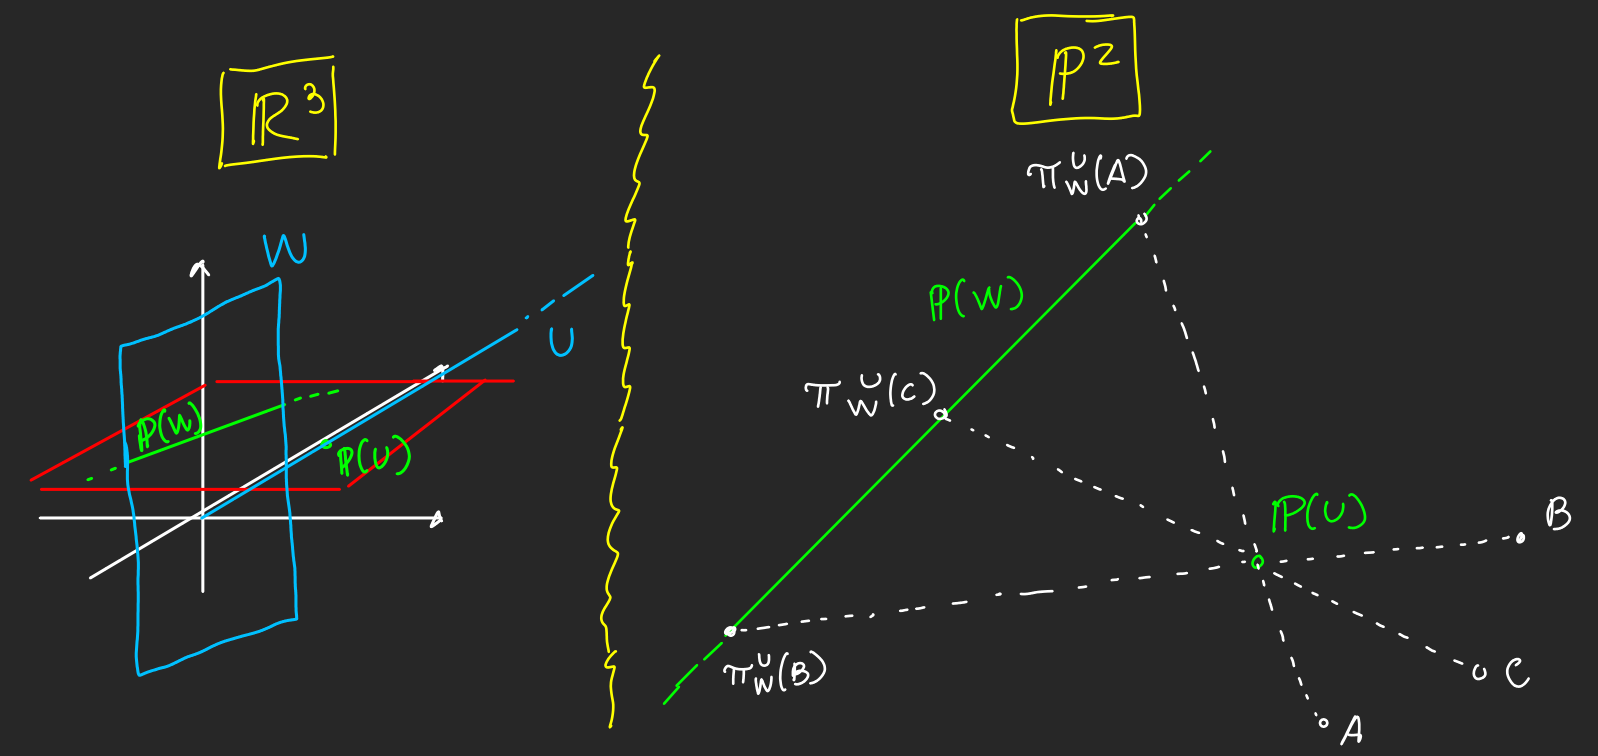
\includegraphics[width=1\textwidth,center]{proiezione.png}
   	 	\label{fig:6}
   	 	\caption{La rappresentazione geometrica di una proiezione per come l'abbiamo appena definita è proprio la proiezione a cui siamo abituati dal liceo!}
   	 \end{figure}
   	 In realtà le proiezioni centrali sono mappe sorprendentemente generali, vediamo il seguente esempio:
   	 \begin{example}[Spazi isomorfi per proiezione]
   	 	Dati due spazi $W_1\oplus W_2=V$ della stessa dimensione, e un altro spazio $U$ tale che $$U\oplus W_1=V$$
   	 	$$U\oplus W_2=V$$
   	 	allora possiamo definire un isomorfismo tra $W_1$ e $W_2$ soltanto usando proiezioni, infatti se restringiamo $\pi_{W_2}^U$ a $W_1$, dato che il kernel è $U$ abbiamo chiaramente una funzione biettiva:
   	 	$$F:\PP(W_1)\setminus\PP(U)\to \PP(W_2)$$
   	 	ma dato che $\PP(W_1)\cap \PP(U)=\eset$ (dato che sono in somma diretta), abbiamo che $F$ è un isomorfismo da $W_1$ a $W_2$.
   	 \end{example}
   	 \begin{figure}[h]
   	 	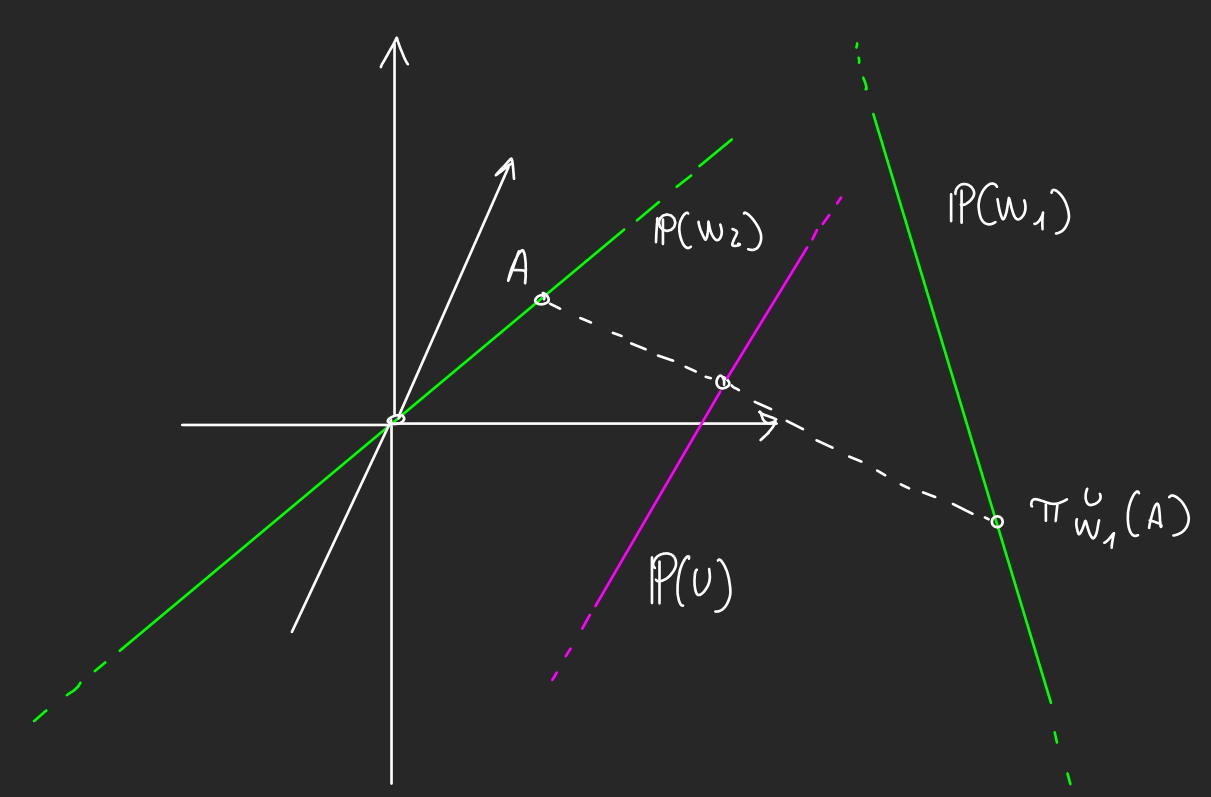
\includegraphics[width=0.8\textwidth,center]{IsomorfismoProiezione.png}
   	 	\label{fig:7}
   	 	\caption{Il caso specifico in $\PP^3$ dell'esempio visto sopra. Le due rette sghembe $\PP(W_1)$ e $\PP(W_2)$ generano $\PP^3$, e la proiezione avviene tramite la retta (sghemba ad entrambe, di nuovo) $\PP(U)$.}
   	 \end{figure}
   	 Questo motiva la seguente proposizione:
   	 \begin{proposition}[Costruire isomorfismi per proiezioni]
   	 	Se $W_1$ e $W_2$ sono due spazi in somma diretta e con la stessa dimensione allora per ogni isomorfismo $F:\PP(W_1)\to \PP(W_2)$ esiste uno spazio $U$ tale che l'applicazione tra spazi vettoriali $\pi_{W_2}^U\mid_{W_1}$ induce l'applicazione $F$ tra spazi proiettivi.  
   	 \end{proposition}
   	 \begin{proof}
   	 	Sia $w_1,w_2,\dots,w_s$ una base di $W_1$ allora definiamo la base di $U$ come
   	 	$$u_i:=w_i-\varphi(w_i)$$
   	 	chiaramente abbiamo che i vettori $u_i$ sono linearmente indipendenti, infatti abbiamo che se esistessero $\alpha_i$ per cui una combinazione degli $u_i$ è nulla usando la linearità di $\varphi$ otterremmo
   	 	$$\varphi(\alpha_1w_1+\dots+\alpha_sw_s)=\alpha_1w_1+\dots+\alpha_sw_s$$
   	 	che implica che gli $\alpha_i$ siano tutti $0$ in quanto $\varphi$ va da $W_1$ a $W_2$ inoltre $W_1\cap W_2=\left\{0\right\}$. D'altra parte per lo stesso motivo abbiamo $U\cap W_1=\left\{0\right\}$, e $U\cap W_2=\left\{0\right\}$, quindi abbiamo che $U$ è in somma diretta sia con $W_1$ che con $W_2$, e questo ci permette di applicare direttamente la costruzione fatta all'esempio precedente.
   	 \end{proof}
   	 \subsubsection{Cambi di coordinate}
   	 Nella sezione precedente abbiamo introdotto il concetto di coordinata proiettiva, in questa sezione parliamo dei cambi di coordinate. Abbiamo già definito l'applicazione, data una base proiettiva ordinata $\mathcal{B}$:
   	 $$\varphi_\mathcal{B}:\PP(V)\to \PP^n$$
   	 che associa ad ogni punto la sua rappresentazione nelle coordinate di $\mathcal{B}$:
   	 \begin{proposition}[Il cambio di coordinate è un isomorfismo]
   	 	L'applicazione $\varphi_\mathcal{B}$ definita sopra è un isomorfismo proiettivo per ogni base proiettiva $\mathcal{B}$.
   	 \end{proposition}
   	 \begin{proof}
   	 	Discende chiaramente dal fatto che l'applicazione lineare associata all'applicazione proiettiva è un isomorfismo.
   	 \end{proof}
   	 In questo modo possiamo definire:
   	 \begin{definition}[Matrice associata ad una proiettività]
   	 	Dati due sistemi di riferimento proiettivi $\mathcal{B}$ e $\mathcal{B}'$ e un'applicazione proiettiva $F:\PP(V)\to\PP(W)$ possiamo definire il \textit{cambio di coordinate} rispetto a questa base come
   	 	$$T:=\varphi_\mathcal{B'}\circ F\circ \varphi_\mathcal{B}^{-1}$$
   	 	in modo analogo a quanto fatto per il cambio di base. Notiamo che $T$ è una trasformazione da $\PP^m$ a $\PP^n$, dunque sarà canonicamente rappresentabile come una matrice, per quanto dimostrato all'inizio sulle trasformazioni lineari tuttavia $F$ e $F'$ sono la stessa trasformazione proiettiva se esiste uno scalare $\lambda\in K^*$ tale che
   	 	$$F=F'\lambda$$
   	 	e quindi allo stesso modo dobbiamo considerare che $T$ non è una singola matrice, ma una classe di equivalenza di matrici, in particolare possiamo definire il \textit{gruppo proiettivo generale} come
   	 	$$T\in \text{PGL}_{n+1}(K):=\faktor{\GL_{n+1}(K)}{K^*}.$$ 
   	 \end{definition}
   	 La proprietà più utile del cambio di coordinate è probabilmente la seguente:
   	 \begin{proposition}[Gli isomorfismi preservano il reticolo]
   	 	Per ogni termine $A$, $B$ e isomorfismo proiettivo $F:\PP(V)\to\PP(W)$ abbiamo che
   	 	$$F\left(A\land B\right)=F(A)\land F(B)$$
   	 	$$F\left(A\lor B\right)=F(A)\lor F(B)$$
   	 	ovvero $F$ preserva la struttura del reticolo.
   	 \end{proposition}
   	 \begin{proof}
   	 	Essenzialmente per definizione di trasformazione proiettiva.
   	 \end{proof}
   	 Questo vuol dire che essenzialmente tutte le proprietà che dipendono solo dalla struttura di reticolo di $\PP^n$ possono essere dimostrate mettendoci in un sistema di riferimento "comodo", in cui i punti principali con cui stiamo lavorando hanno coordinate $(1:0:\dots:0),(0:1:\dots:0),\dots,(0:0:\dots:1),(1:1:\dots:1)$.
   	 \subsubsection{I teoremi di Pappo e Desargues}
   	 Vediamo i seguenti tre teoremi\footnote{Le rappresentazioni geometriche di questi teoremi sono tutte e tre molto famose, non verranno inserite immagini qui, ma si consiglia il lettore di cercare su internet per capire cosa stiano facendo \textit{geometricamente} gli oggetti con cui stiamo lavorando.} per esercitarci con i concetti introdotti finora:
   	 \begin{theorem}[Pappo]
   	 	Siano $r,s\subseteq \PP^2$ due rette, siano $A,B,C$ tre punti su $s$ e $A',B',C'$ tre punti su $r$ allora i tre punti di intersezione
   	 	\begin{gather*}
   	 		\overline{A'C}\land \overline{AC'} \\
   	 		\overline{A'B}\land \overline{AB'} \\
   	 		\overline{B'C}\land \overline{BC'}
   	 	\end{gather*}
   	 	sono allineati.
   	 \end{theorem}
   	 \begin{proof}
   	 	Per quanto detto prima esiste sempre un'intersezione tra $r$ ed $s$. Assumiamo WLOG che abbia coordinate $(1:0:0)$, così come assumiamo che $A$ abbia coordinate $(0:1:0)$ e $A'$ abbia coordinate $(0:0:1)$. 
   	 	\begin{remark}[Congiunzioni di punti e intersezioni di rette con prodotti vettoriali]
   	 		Dati due punti 
   	 		$$p=(x_1:x_2:x_3)$$
   	 		$$q=(y_1:y_2:y_3)$$
   	 		la retta passante per questi in $\PP^2$ sarà del tipo 
   	 		$$a_1X_1+a_2X_2+a_3X_3=0$$
   	 		dove gli $a_i$ soddisferanno
   	 		$$(a_1:a_2:a_3)=\left(\left(p\times q\right)_1:\left(p\times q\right)_2:\left(p\times q\right)_3\right)$$
   	 		in modo simile possiamo scrivere l'intersezione di due rette proiettive 
   	 		$$a_1X_1+a_2X_2+a_3X_3=0$$
   	 		$$b_1X_1+b_2X_2+b_3X_3=0$$
   	 		con un prodotto vettoriale:
   	 		$$\left(\left(a\times b\right)_1:\left(a\times b\right)_2:\left(a\times b\right)_3\right)$$
   	 		dove $a$ e $b$ sono le liste rispettivamente degli $a_i$ e dei $b_i$.
   	 	\end{remark}
   	 	Notiamo che per come abbiamo messo i punti la retta $r$ avrà equazione 
   	 	$$X_3=0$$
   	 	e analogamente la retta $s$ avrà equazione
   	 	$$X_0=0$$
   	 	dunque possiamo scrivere i punti $B,B',C,C'$ come
   	 	$$B=(1:b:0)$$
   	 	$$B'=(1:0:b')$$
   	 	$$C=(1:c:0)$$
   	 	$$C'=(1:0:c')$$
   	 	dunque per calcolare le intersezioni e le congiunzioni possiamo usare il trucco del prodotto scalare visto sopra:
   	 	$$P_1=\left(A\lor B'\right)\land \left(A'\lor B\right)=\left(A'\times B\right)\times \left(A\times B'\right)=(-1:-b:-b')$$
   	 	$$P_2=\left(A\lor C'\right)\land \left(A'\lor C\right)=\left(A'\times C\right)\times \left(A\times C'\right)=(-1:-c:-c')$$
   	 	$$P_3=\left(C\lor B'\right)\land \left(C'\lor B\right)=\left(C'\times B\right)\times \left(C\times B'\right)=(bb'-cc':bc(b'-c'):b'c'(b-c))$$
   	 	ora non resta che controllare se questi tre punti sono allineati. Abbiamo due modi di vedere la verifica che stiamo per fare: la prima è che chiaramente se consideriamo i vettori con coordinate deomogeneizzate quelle dei punti $P_i$ allora se la loro congiunzione è una retta proiettiva nello spazio affine deomogeneizzato deve essere un piano, e quindi dobbiamo imporre che la matrice avente righe o colonne $P_1, P_2,P_3 $ abbia determinante $0$. L'altro modo è considerare il sistema di equazioni parametriche della congiunzione dei tre punti:
   	 	$$\begin{pmatrix}
   	 		-1 & -1 & bb'-cc' \\
   	 		-b & -c & bc(b'-c')\\
   	 		-b'& -c'& b'c'(b-c)
   	 	\end{pmatrix}\begin{pmatrix}
   	 	t_1 \\
   	 	t_2 \\
   	 	t_3
   	 	\end{pmatrix}=
   	 	\begin{pmatrix}
   	 		X_1 \\
   	 		X_2 \\
   	 		X_3
   	 	\end{pmatrix}$$
   	 	se $X_1,X_2,X_3$ sono allineati la matrice deve avere rango $2$, e quindi di nuovo il determinante deve essere $0$. D'altra parte notiamo che se $C_i$ sono le colonne di quella matrice abbiamo
   	 	$$C_3=cc'C_1-bb'C_2$$
   	 	e quindi il determinante sarà $0$, il che implica la tesi.
   	 \end{proof}
   	 \begin{definition}[Triangolo non degenere]
   	 	Siano $A,B,C$ punti in $\PP^n$. Diciamo che $ABC$ è un triangolo \textit{non degenere} se $A\lor B\lor C$ ha dimensione $2$.
   	 \end{definition}
   	 \begin{definition}[Prospettività per un punto e per una retta]
   	 	Prendiamo due triangoli $ABC,A'B'C'\in\PP^n$. Diciamo che i due triangoli sono \textit{prospettivi rispetto a un punto} se 
   	 	$$\left(A\lor A'\right)\land\left(B\lor B'\right)\land \left(C \lor C'\right)\ne \eset$$
   	 	ovvero se le rette del tipo $AA'$ concorrono in un punto, cioè se esiste una proiezione centrale che manda un triangolo nell'altro. Analogamente diciamo che i due triangoli sono \textit{prospettivi per una retta} se i tre punti
   	 	$$\left(A\lor B\right)\land\left(A'\lor B'\right)$$
   	 	$$\left(C\lor B\right)\land\left(C'\lor B'\right)$$
   	 	$$\left(A\lor C\right)\land\left(A'\lor C'\right)$$
   	 	sono allineati, ovvero la loro congiunzione ha dimensione $1$. Anche questo è equivalente a dire che esiste una proiezione per una certa retta che manda un triangolo nell'altro.
   	 \end{definition}
   	 \begin{theorem}[Desargues debole]
   	 	Siano $ABC,A'B'C'$ triangoli non degeneri in $\PP^2$, allora sono prospettivi rispetto ad una retta se e solo se sono prospettivi rispetto ad un punto.
   	 \end{theorem}
   	 \begin{proof}
   	 	Siano $x_1,x_2,x_3$ i vettori deomogeneizzati corrispondenti ai punti $A,B,C$ e $y_1,y_2,y_3$ i vettori deomogeneizzati corrispondenti ai punti $A',B',C'$. Supponiamo che i due triangoli siano prospettivi rispetto ad un punto. se chiamiamo $p$ il vettore deomogeneizzato dell'intersezione abbiamo che devono esistere coefficienti $\alpha_i$ e $\beta_i$ tali che
   	 	$$\alpha_1x_1-\beta_1y_1=p$$
   	 	$$\alpha_2x_2-\beta_2y_2=p$$
   	 	$$\alpha_3x_3-\beta_3y_3=p$$
   	 	da cui uguagliando
   	 	$$\alpha_1x_1-\beta_1y_1=\alpha_2x_2-\beta_2y_2$$
   	 	$$\alpha_1x_1-\beta_1y_1=\alpha_3x_3-\beta_3y_3$$
   	 	$$\alpha_3x_3-\beta_3y_3=\alpha_2x_2-\beta_2y_2$$
   	 	ovvero riordinando i termini
   	 	$$\alpha_1x_1-\alpha_2x_2=\beta_1y_1-\beta_2y_2$$
   	 	$$\alpha_1x_1-\alpha_3x_3=\beta_1y_1-\beta_3y_3$$
   	 	$$\alpha_3x_3-\alpha_2x_2=\beta_3y_3-\beta_2y_2$$
   	 	d'altra parte la prima equazione ci sta dicendo che $(A\lor B)\land(A'\lor B')$ è non vuota ed è uguale a
   	 	$$\PP\left(\langle \alpha_1x_1-\alpha_2x_2 \rangle\right)$$
   	 	e così analogamente le altre due
   	 	$$\PP\left(\langle \alpha_1x_1-\alpha_3x_3 \rangle\right)$$
   	 	$$\PP\left(\langle \alpha_3x_3-\alpha_2x_2 \rangle\right)$$
   	 	ma d'altra parte la congiunzione di questi tre ha dimensione $1$, in quanto sono linearmente dipendenti (la somma è $0$), quindi abbiamo un verso della tesi.\footnote{E questo sarebbe sufficiente a concludere applicando il principio della dualità proiettiva, che vedremo più avanti.} \\
   	 	Assumiamo ora che i tre punti siano prospettivi rispetto ad una retta, allora esisteranno tre punti $p_1,p_2,p_3$ sulla retta tali che
   	 	\begin{gather*}
   	 		\alpha_1x_1+\alpha_2x_2=\alpha_3y_1+\alpha_4y_2=p_1 \\
   	 		\beta_1x_2+\beta_2x_3=\beta_3y_2+\beta_4y_3=p_2 \\
   	 		\gamma_1x_1+\gamma_2x_3=\gamma_3y_1+\gamma_4y_3=p_3
   	 	\end{gather*}
   	 	dunque dato che abbiamo assunto che $p_1,p_2,p_3$ sono allineati, e dato che ogni vettore singolarmente sicuramente non è $0$, dobbiamo avere tre scalari $\tau_1,\tau_2,\tau_3\in K$ tali che al più uno di questi è nullo, e inoltre
   	 	$$\tau_1p_1+\tau_2p_2+\tau_3p_3=0$$
   	 	ovvero
   	 	\begin{gather*}
   	 		\tau_1\left(\alpha_1x_1+\alpha_2x_2\right)+\tau_2\left(\beta_1x_2+\beta_2x_3\right)+\tau_3\left(\gamma_1x_1+\gamma_2x_3\right)=0 \\
   	 		\tau_1\left(\alpha_3y_1+\alpha_4y_2\right)+\tau_2\left(\beta_3y_2+\beta_4y_3\right)+\tau_3\left(\gamma_3y_1+\gamma_4y_3\right)=0
   	 	\end{gather*}
   	 	ora l'idea è usare il fatto che gli $x_i$ sono indipendenti tra loro, così come gli $y_i$. Dividiamo in due casi:
   	 	\begin{itemize}
   	 		\item Se uno dei $\tau_i$ è $0$, assumiamo WLOG $\tau_1$, allora confrontando i coefficienti di $x_1$ nella prima equazione e di $y_1$ nella seconda abbiamo 
   	 		$$\tau_3\gamma_1=0$$
   	 		$$\tau_3\gamma_3=0$$
   	 		da cui concludiamo che $\gamma_1=\gamma_3=0$ questo vuol dire che 
   	 		$$\gamma_2x_3=p_3=\gamma_4y_3$$
   	 		cioè abbiamo che due vertici dei triangoli coincidono ($C=C'$) e quindi sono banalmente prospettici rispetto a $(B\lor B')\land (A\lor A')$, che esiste sempre dato che siamo in $\PP^2$. In modo analogo abbiamo $A=A'$ o $B=B'$ se imponiamo nulli gli altri $\tau_i$.
   	 		\item Se tutti i $\tau_i$ sono diversi da $0$ i vettori 
   	 		$$\frac{p_1}{\tau_1},\frac{p_2}{\tau_2},\frac{p_3}{\tau_3}$$
   	 		corrispondono agli stessi punti proiettivi di $p_1,p_2,p_3$, quindi possiamo scegliere dei nuovi $\alpha_i,\beta_i$ e $\gamma_i$ tali che
   	 		\begin{gather*}
   	 			\alpha_1x_1+\alpha_2x_2+\beta_1x_2+\beta_2x_3+\gamma_1x_1+\gamma_2x_3=0 \\
   	 			\alpha_3y_1+\alpha_4y_2+\beta_3y_2+\beta_4y_3+\gamma_3y_1+\gamma_4y_3=0
   	 		\end{gather*}
   	 		ma di nuovo dato che i $x_i$ e $y_i$ sono linearmente indipendenti abbiamo un sacco di uguaglianze, in particolare le equazioni dei punti $p_i$ si riscrivono come
   	 		\begin{gather*}
   	 			\mu_1x_1+\mu_2x_2=\lambda_1y_1+\lambda_2y_2=p_1 \\
   	 			-\mu_2x_2+\mu_3x_3=-\lambda_2y_2+\lambda_3y_3=p_2 \\
   	 			-\mu_1x_1-\mu_3x_3=-\lambda_1y_1-\lambda_3y_3=p_3
   	 		\end{gather*}
   	 		dove abbiamo definito dei nuovi coefficienti opportuni $\mu_i$ e $\lambda_i$. Riordinando le equazioni otteniamo
   	 		\begin{gather*}
   	 			\mu_1x_1-\lambda_1y_1=\lambda_2y_2-\mu_2x_2 \\
   	 			\mu_3x_3-\lambda_3y_3=\mu_2x_2-\lambda_2y_2 \\
   	 			\mu_1x_1-\lambda_1y_1=\lambda_3y_3-\mu_3x_3
   	 		\end{gather*}
   	 		che uguagliando tutto ci dicono proprio che le rette $(x_1,y_1)$, $(x_2,y_2)$ e $(x_3,y_3)$ si intersecano in un solo punto, come richiesto.
   	 	\end{itemize}
   	 	Dunque in ogni caso arriviamo alla tesi, e abbiamo finito.
   	 \end{proof}
   	 La versione più generale di questo teorema è la seguente:
   	 \begin{theorem}[Desargues forte]
   	 	Dati due triangoli non degeneri $ABC$ e $A'B'C'$ in $\PP^n$ questi sono prospettivi rispetto ad un punto se e solo se lo sono rispetto ad una retta.
   	 \end{theorem}
   	 \begin{proof}
   	 	Siano $\pi$ e $\pi'$ i piani contenenti i triangoli $ABC$ e $A'B'C'$. Se $\pi=\pi'$ possiamo brutalmente applicare Desargues debole, quindi assumiamo che $\pi\ne \pi'$, dimostriamo un'implicazione alla volta:
   	 	\begin{description}
   	 		\item[Punto$\implies$Retta] Se esiste un punto in 
   	 		$$\left(A\lor A'\right)\land \left(B\lor B'\right)\land \left(C\lor C'\right)$$
   	 		allora vuol dire che i punti $A,A',B,B'$ sono complanari, ovvero le rette $AB$ e $A'B'$ sono complanari, dunque il loro punto di intersezione esiste, in particolare il punto
   	 		$$\left(B\lor A\right)\land \left(B'\lor A'\right)$$
   	 		apparterrà contemporaneamente a $\pi$ e $\pi'$, cioè apparterrà a $\pi\land \pi'$. Analogamente si può dire dei punti di intersezione delle rette $AC$ e $A'C'$, così come si può dire per l'intersezione delle rette $BC$ e $B'C'$. Ma dato che $\pi\ne\pi'$ abbiamo che questi tre punti appartengono tutti allo spazio $\pi\land \pi'$, che è tale che
   	 		$$\dim \pi\land \pi'\le 1$$
   	 		dunque sono allineati.
   	 		\item[Retta$\implies$Punto] Assumiamo che i triangoli siano prospettivi rispetto ad una retta, allora abbiamo che $A,A',B,B'$ sono complanari, sia $\pi''$ il piano che li contiene. Le rette $AA'$ e $BB'$ sono complanari, quindi si intersecano in un punto che chiamiamo $P_1\in\pi''$. Per lo stesso motivo esisterà un'intersezione $P_2$ delle rette $AA'$ e $CC'$ così come un'intersezione $P_3$ delle rette $BB'$ e $CC'$. \\
   	 		Ma allora abbiamo
   	 		$$P_3\in BB'\subseteq \pi''$$
   	 		e
   	 		$$P_2\in AA'\subseteq \pi''$$ 
   	 		ma $P_3,P_2\in CC'$, quindi se per assurdo avessimo $P_3\ne P_2$ avremmo $CC'\subseteq \pi''$ cioè tutti i punti $A,B,C,A',B',C'$ appartengono ad uno stesso piano, assurdo. Dunque abbiamo 
   	 		$$P_1=P_2=P_3=AA'\land BB'\land CC'$$
   	 		come volevamo
   	 	\end{description}
   	 	Dunque abbiamo dimostrato tutte le implicazioni, e abbiamo finito.
   	 \end{proof}
   	 \subsubsection{Affinità che inducono proiettività}
   	 Con gli spazi vettoriali avevamo visto chiaramente che definendo una trasformazione di due basi degli spazi $V$ e $W$ si definiva automaticamente una trasformazione degli spazi $V$ e $W$. In proiettiva questa cosa è analoga, ma un po' più complicata:
   	 \begin{theorem}[Moving Points]
   	 	Siano $V$ e $W$ spazi vettoriali di dimensione $n+1$ su un campo $K$ \textbf{infinito}. Preso un sistema di riferimento proiettivo $P_0,P_1,\dots,P_{n+1}$ dello spazio $\PP(V)$, se $Q_0,Q_1,\dots,Q_{n+1}$ sono $n+2$ punti di $\PP(W)$ tali che
		$$r=\dim\left(Q_0\lor Q_1\lor \dots \lor Q_{n+1}\right)$$
   	 	e inoltre si abbia che comunque scelti $r+1$ questi generano uno spazio di dimensione $r$, allora esiste una trasformazione 
   	 	\begin{align*}
   	 		F:\PP(V)&\to\PP(W) \\
   	 		P_i & \mapsto Q_i
   	 	\end{align*}
   	 	per ogni $0\le i\le r+1$. In particolare se $r=n$ questa trasformazione è anche unica.
   	 \end{theorem}
   	 \begin{proof}
   	 	Per come abbiamo definito i sistemi di riferimento proiettivi possiamo scrivere 
   	 	\begin{gather*}
   	 		\langle v_0\rangle=P_0 \\
   	 		\langle v_1\rangle=P_1 \\
   	 		\vdots \\
   	 		\langle v_n\rangle=P_n \\
   	 		\langle v_0+v_1+\dots+v_n\rangle =P_{n+1}
   	 	\end{gather*}
   	 	grazie al fatto che $P_0\oplus P_1\oplus \dots\oplus P_n=V$. Siano $w_0,\dots,w_n,w_{n+1}$ i vettori associati ai punti $Q_0,\dots,Q_{n},Q_{n+1}$, è ben noto che per ogni lista $\mu_0,\mu_1,\dots,\mu_n\in K^*$ di scalari diversi da $0$ possiamo trovare un'applicazione lineare $\varphi:V\to W$ tale che
   	 	$$\varphi(v_i)=\mu_iw_i$$
   	 	per ogni $i$. A questa applicazione sono associate evidentemente tante trasformazioni proiettive che mandano i punti $P_0,\dots,P_n$ nei punti $Q_0,\dots,Q_n$, rimangono tuttavia da sistemare i punti $P_{n+1}$ e $Q_{n+1}$. Ciò è equivalente a chiedere che sia soddisfatta la seguente relazione
   	 	$$\mu_{n+1}w_{n+1}=\varphi(v_{n+1})=\varphi\left(\sum_{i=0}^{n}v_i\right)=\sum_{i=0}^{n}\varphi(v_i)=\sum_{i=0}^{n}\mu_i w_i$$
   	 	ovvero stiamo cercando $\mu_0,\mu_1,\dots,\mu_n,\mu_{n+1}\in K^*$ tali che soddisfino la seguente equazione:
   	 	$$
   	 	\left(
   	 	\begin{array}{c|c|c|c}
   	 		&&&\\
   	 		w_0 & w_1 & \dots & w_n\\
   	 		&&&
   	 	\end{array}
   	 	\right)\begin{pmatrix}
   	 		\mu_0 \\
   	 		\vdots \\
   	 		\mu_n
   	 	\end{pmatrix}=\mu_{n+1}w_{n+1}
   	 	$$
   	 	ovvero
   	 	$$A\mu=
   	 	\left(
   	 	\begin{array}{c|c|c|c|c}
   	 		&&&\\
   	 		w_0 & w_1 & \dots & w_n & w_{n+1}\\
   	 		&&&
   	 	\end{array}
   	 	\right)
   	 	\begin{pmatrix}
   	 	\mu_0 \\
   	 	\vdots \\
   	 	\mu_n \\
   	 	-\mu_{n+1}
   	 	\end{pmatrix}=0
   	 	$$
   	 	d'altra parte il rango di quella matrice è per ipotesi proprio $r+1$ (uno più della dimensione dello spazio proiettivo generato dai punti $Q_i$), quindi dato che 
   	 	$$r+1\le n+2$$
   	 	abbiamo sempre almeno un elemento del kernel, ovvero una scelta dei $\mu_i$ che soddisfa le condizioni di cui abbiamo bisogno. In particolare se $r=n$ abbiamo
   	 	$$\dim \ker{A}=n+2-n-1=1$$
   	 	cioè la soluzione è unica a meno di riscalare tutti i $\mu_i$ per un fattore costante, ovvero la trasformazione proiettiva associata a $\varphi$ è unica.
   	 \end{proof}
   	 Nell'ambito delle olimpiadi della matematica questo è il principio che sta alla base della tecnica dei "moving points", che dice che se due trasformazioni proiettive coincidono su $n+2$ coppie di punti allora sono identiche. \\
   	 Per gli spazi affini avevamo visto che ci era spesso comodo introdurre una prima coordinata "ausiliaria" $X_0$ all'inizio delle liste ordinate di numeri che usavamo, in modo che segnalasse se quello con cui stavamo lavorando fosse un punto o un vettore. Questo ad esempio ci era servito per trovare una forma sintetica delle trasformazioni affini:
   	 \begin{align*}
   	 	\left(\begin{array}{c}
   	 		1 \\
   	 		\hline
   	 		x
   	 	\end{array}\right)\mapsto 
   	 	\left(
   	 	\begin{array}{c}
   	 		1 \\
   	 		\hline
   	 		Ax+b
   	 	\end{array}\right)=\left(\begin{array}{c}
   	 	1 \\
   	 	\hline
   	 	x
   	 	\end{array}\right)\left(
   	 	\begin{array}{c|c}
   	 		1 & 0 \\
   	 		\hline
   	 		b & A
   	 	\end{array}
   	 	\right)
   	 \end{align*}
   	 $$$$
   	 In proiettiva questo passaggio è quasi automatico, in effetti pensiamo all'omogeneizzazione della coordinata $0$:
   	 \begin{align*}
   	 	\varphi_0:\AA^n\to \,&\PP^n \\
   	 	\left(\begin{array}{c}
   	 		1 \\
   	 		\hline 
   	 		y_1 \\
   	 		y_2 \\
   	 		\vdots \\
   	 		y_n
   	 	\end{array}\right) \mapsto & (1:y_1:y_2:\dots:y_n)=(X_0:X_1:\dots:X_n)
   	 \end{align*}
   	 In altre parole in proiettiva i punti all'infinito si comportano naturalmente come vettori, mentre i punti con la prima coordinata non $0$ si comportano naturalmente come punti. Questo vuol dire che ad ogni affinità $\AA^n\to\AA^n$ possiamo associare una proiettività $\PP^n\to\PP^n$ semplicemente copiando la matrice ed eliminando i "bordi" che avevamo artificiosamente introdotto nel caso affine.
   	 \begin{lemma}[Da Proiettività ad Affinità e viceversa]
   	 	Le trasformazioni proiettive $F:\PP^n\to\PP^n$ indotte da affinità sono tutte e sole quelle che hanno una matrice della forma
   	 	$$
   	 	\left(
   	 	\begin{array}{c|c}
   	 		1 & 0 \\
   	 		\hline 
   	 		b & A
   	 	\end{array}
   	 	\right)
   	 	$$
   	 \end{lemma}
   	 \begin{proof}
   	 	Andare dalle affinità alle proiettività è semplice: presa la matrice di una affinità di $U_0$ basta omogeneizzare la coordinata $0$ per ottenere la matrice di una proiettività indotta. Prendiamo ora una trasformazione proiettiva, vogliamo capire quando avviene che 
   	 	$$F(U_0)=U_0$$
   	 	i punti di $U_0$ sono tutti della forma
   	 	$$(1:x_1:\dots:x_n)$$
   	 	dunque presa una matrice $A$ di $F$ vogliamo che
   	 	$$A(1:x_1:\dots:x_n)=(1:y_1:\dots:y_1)$$
   	 	dunque scriviamo la matrice $A$ come
   	 	$$
   	 	\left(
   	 	\begin{array}{c|c}
   	 		k & v^\intercal \\
   	 		\hline
   	 		b & B
   	 	\end{array}
   	 	\right)
   	 	$$
   	 	perchè $A(U_0)=U_0$ dunque dobbiamo avere che per ogni scelta di $x$ la prima coordinata del vettore $A\begin{pmatrix}
   	 		1 \\
   	 		\hline
   	 		x
   	 	\end{pmatrix}$ sia uguale a $1$, ovvero per ogni $x$ deve valere
   	 	$$
   	 	\left(
   	 	\begin{array}{c|c}
   	 		k & v^\intercal \\
   	 		\hline
   	 		b & B
   	 	\end{array}
   	 	\right)
   	 	\left(
   	 	\begin{array}{c}
   	 		X \\
   	 		\hline
   	 		x
   	 	\end{array}
   	 	\right)=
   	 	\left(
   	 	\begin{array}{c}
   	 		Y \\
   	 		\hline
   	 		y
   	 	\end{array}
   	 	\right)
   	 	$$
   	 	che vuol dire che per ogni $x$ deve valere
   	 	$$kX+v^\intercal x =Y\ne 0$$
   	 	questo è possibile solo se $v=0$ e $k\ne 0$, ovvero la matrice è equivalente ad una della forma (riscalando tutto per $1/k$):
   	 	$$
   	 	\left(
   	 	\begin{array}{c|c}
   	 		1 & 0 \\
   	 		\hline
   	 		b/k & B/k
   	 	\end{array}
   	 	\right)
   	 	$$
   	 	come volevamo mostrare.
   	 \end{proof}
   	 
   	 \subsection{Principio della dualità proiettiva}
   	 Quando avevamo parlato degli spazi duali avevamo introdotto il concetto di dualità canonica, che poi ha essenzialmente coinciso con il concetto di prodotto scalare standard. Avevamo introdotto il sottospazio $W^\perp$ in due modi: uno come sottospazio ortogonale rispetto al prodotto scalare e l'altro come sottospazio del duale ortogonale rispetto alla dualità canonica. In questa sezione lo spazio $W^\perp$ sarà da intendersi rispetto alla dualità canonica, così come i simboli $\langle \cdot ,\cdot \rangle$ saranno da intendersi come dualità canoniche. 
   	 \begin{definition}[Dualità proiettiva]
   	 	La mappa tra i reticoli $\bot:S(V)\to S(V^*)$ tale che
   	 	$$W\mapsto W^\perp$$
   	 	si dice \textit{dualità proiettiva}.
   	 \end{definition}
   	 \begin{example}[Ortogonali proiettivi]
   	 	Prendiamo un $W$ il piano di $K^3$ di equazione 
   	 	$$x_0+x_1-x_2=0$$
   	 	vogliamo trovare $W^\perp$. Per fare ciò ci basta imporre che per ogni $w\in W$ valga
   	 	$$\langle \varphi,w\rangle=0$$
   	 	ovvero, dato che gli elementi del duale sono tutti della forma
   	 	$$\begin{pmatrix}
   	 		a_0 \\
   	 		a_1 \\
   	 		a_2
   	 	\end{pmatrix}^*\begin{pmatrix}
   	 	x_0 \\
   	 	x_1 \\
   	 	x_2
   	 	\end{pmatrix}=a_0x_0+a_1x_1+a_2x_2$$
   	 	ci basta avere che 
   	 	
   	 \end{example}
   	 \begin{proposition}[principio della dualità proiettiva]
   	 	Per ogni $W,W_1,W_2\in S(V)$ allora rispetto alla dualità proiettiva valgono le seguenti proposizioni:
   	 	\begin{itemize}
   	 		\item Se $W_1\le W_2$ allora 
   	 		$$W_1^\perp \ge W_2^\perp.$$
   	 		\item Se $\PP(W)=\PP(W_1)\lor \PP(W_2)$ allora 
   	 		$$\PP(W^\perp)=\PP(W_1^\perp)\land \PP(W_2^\perp).$$
   	 		\item Se $\PP(W)=\PP(W_1)\land \PP(W_2)$ allora
   	 		$$\PP(W^\perp)=\PP(W_1^\perp)\lor \PP(W_2^\perp).$$
   	 		\item Avevamo già visto infine che 
   	 		$$\dim \PP(W^\perp)=\dim \PP(V)-\dim \PP(W)-1.$$
   	 	\end{itemize}
   	 	questo vuol dire che essenzialmente abbiamo un algoritmo che per ogni proposizione vera in ogni spazio proiettivo $V$ produce un'altra proposizione vera in ogni spazio $V^*$ ad esso isomorfo (e quindi vera anche in $V$) semplicemente sostituendo 
   	 	\begin{align*}
   	 		\le\,   \mapsto  & \ge \\
   	 		\land \mapsto  & \lor \\
   	 		\lor  \mapsto  & \land \\
   	 		\dim  \mapsto  & \dim\PP(V)-\dim -1
   	 	\end{align*}
   	 \end{proposition}
   	 \begin{example}[Punti all'infinito]
   	 	Un primo esempio di applicazione del principio di dualità proiettiva è tra le seguenti due proposizioni:
   	 	\begin{itemize}
   	 		\item Per ogni coppia di punti in uno spazio proiettivo di dimensione $2$ esiste ed è unica la retta passante per essi.
   	 		\item Per ogni coppia di rette in uno spazio proiettivo di dimensione $2$ esiste ed è unico il loro punto di intersezione. 
   	 	\end{itemize}
   	 \end{example}
   	 Facciamo ancora un po' di esercizio con il principio di Dualità proiettivo:
   	 \begin{proposition}[Retta per un punto e due rette]
   	 	\label{Retta per un punto e due rette}
   	 	Se $r,s$ sono rette disgiunte in $\PP^3$ e $P\in \PP^3$ è un punto né su $r$ né su $s$ esiste un'unica retta $l$ incidente a $r$ e ad $s$ e passante per $P$.
   	 \end{proposition}
   	 \begin{proof}[Dimostrazione - Geometria]
   	 	Dobbiamo dimostrare che l'insieme
   	 	$$l=\Pi_1\land \Pi_2$$
   	 	con 
   	 	$$\Pi_1=r\lor P$$
   	 	$$\Pi_2=s\lor P$$
   	 	ha dimensione $1$ (il che implica l'unicità), e che l'intersezione sia con $r$ che con $s$ è non vuota. Questo si riduce ad applicare tante volte la formula di Grassmann:
   	 	$$\dim \Pi_1=\dim r + \dim P - \dim P\land r=1+0-(-1)=2$$
   	 	$$\dim \Pi_2=\dim s + \dim P - \dim P\land s=1+0-(-1)=2$$
   	 	dove abbiamo usato il fatto che $P$ non è né su $r$ né su $s$. Dunque applicando di nuovo la formula di Grassmann
   	 	$$\dim \Pi_1\land \Pi_2=\dim \Pi_1+\dim \Pi_2-\dim \Pi_1\lor \Pi_2=2+2-\dim r\lor s\lor P$$
   	 	adesso dobbiamo semplicemente determinare $\dim r\lor s \lor P$, ma questo è facile se consideriamo che
   	 	$$\dim r\lor s \lor P \le \dim \PP^3$$
   	 	e inoltre abbiamo che $\dim r \lor P=2$, quindi 
   	 	$$\dim r \lor s \lor P\ge 2$$
   	 	d'altra parte se fosse esattamente $2$ avremmo un piano che contiene sia $r$ che $s$, quindi sarebbero per forza incidenti, il che è assurdo. Dunque abbiamo $r\lor s\lor P=3$ ovvero
   	 	$$\dim \Pi_1\land \Pi_2=1.$$
   	 	Rimane da dimostrare che 
   	 	$$\dim l \land s\ge 0$$
   	 	$$\dim l \land p\ge 0$$
   	 	ma d'altra parte abbiamo che
   	 	$$l\le r\lor P$$
   	 	$$r\le r\lor P$$
   	 	ovvero il piano $r\lor P$ (di dimensione $2$, come è facile dimostrare con Grassmann) contiene sia $r$ che $l$, cioè sono incidenti. Analogamente si trova per $s$, e quindi abbiamo finito.
   	 \end{proof}
   	 Una dimostrazione alternativa si basa unicamente sull'algebra lineare, e mostra molto bene come la geometria proiettiva sia un sistema molto amichevole, in cui molto spesso esistono più approcci equivalenti allo stesso problema.
   	 \begin{proof}[Dimostrazione - Algebra Lineare]
   	 	Scriviamo esplicitamente chi sono le rette $r$ e $s$, ovvero esistono due piani $V_1$ e $V_2$ tali che
   	 	$$r=\PP(V_1)$$
   	 	$$s=\PP(V_2)$$
   	 	inoltre dato che $r$ ed $s$ sono disgiunte anche $V_1$ e $V_2$ devono essere disgiunti. Questo significa che 
   	 	$$V_1\oplus V_2 = K^4$$
   	 	dato che $V_1$ e $V_2$ hanno dimensione $2$. Consideriamo allora il vettore $v\in K^4$ tale che
   	 	$$P=\PP(\langle v \rangle)$$
   	 	per quanto detto prima possiamo decomporlo come
   	 	$$v=v_1+v_2$$
   	 	dove $v_1\in V_1$ e $v_2\in V_2$, così facendo abbiamo trovato la retta che cercavamo, infatti non è difficile verificare che 
   	 	$$l=\PP\left(\langle\left\{v_1,v_2\right\}\rangle\right)$$
   	 	soddisfa tutte le proprietà richieste.
   	 \end{proof}
   	 Il teorema di Pappo e Desargues...
   	 \begin{lemma}[Aggiunzione Proiettiva]
   	 	Sia $F:\PP^n\to \PP^m$ una trasformazione proiettiva, e $A\in K_{(m+1)\times (n+1)}$ la sua matrice associata, allora la matrice $A^\intercal$ è associata alla trasformazione $F^*:\left(\PP^m\right)^*\to\left(\PP^n\right)^*$ associata all'applicazione lineare trasposta.
   	 \end{lemma}
   	 \begin{proof}
   	 	Prendiamo l'applicazione lineare $\varphi:K^{n+1}\to K^{m+1}$ indotta da $F$, evidentemente abbiamo
   	 	$$\varphi(X)=AX$$
   	 	allora la sua trasposta per definizione è tale che, rispetto alla dualità canonica:
   	 	$$\langle \psi,\varphi v\rangle=\langle \varphi^*\circ \psi,v\rangle$$
   	 	
   	 \end{proof}
   	 \subsection{Birapporti}
   	 Per il momento non abbiamo davvero un modo per codificare il concetto di distanza date solo le coordinate omogenee di un punto. A tale scopo introduciamo la nozione di birapporto, per farlo consideriamo il seguente esempio:
   	 \begin{example}[Trasformazione di M\"obius]
   	 	Siano $(1:a),(1:b),(1:c)$ tre punti in $\PP^1$. Trovare l'unica proiettività $F:\PP^1\to\PP^1$ che manda 
   	 	$$F((1:a))=(0:1)$$
   	 	$$F((1:b))=(1:0)$$
   	 	$$F((1:c))=(1:1)$$
   	 	ovvero, se consideriamo un piano affine $U_0$ ottenuto dalla deomogeneizzazione della prima coordinata stiamo mandando il primo nell'origine del piano affine $U_0$, il secondo nel punto all'infinito e il terzo nel punto $(1:1)$.
   	 \end{example}
   	 \begin{proof}[Soluzione]
   	 	Notiamo che ci basta trovare una funzione $f$ tale che
   	 	$$F((1:x))=(1:f(x))$$
   	 	e per quanto detto prima sulle trasformazioni di M\"obius $f$ sarà il rapporto di due polinomi di primo grado in $x$, in particolare applicando l'interpolazione di Lagrange arriviamo a 
   	 	$$f(x)=\frac{(c-a)(x-b)}{(c-b)(x-a)}$$
   	 	che chiaramente manda $(1:b)$ e $(1:c)$ dove dovrebbero andare, e moltiplicando per il denominatore da entrambi i lati manda anche $(1:a)$ nel punto all'infinito.
   	 \end{proof}
   	 Quindi definiamo
   	 \begin{definition}[Birapporto]
   	 	Dati quattro punti allineati in uno spazio proiettivo, ovvero $a,b,c,d\in \PP^1$ definiamo il loro \textit{birapporto} come l'immagine di $d$ rispetto all'unica proiettività di $\PP^1$ che manda 
   	 	$$a\mapsto (0:1)$$
   	 	$$b\mapsto (1:0)$$
   	 	$$c\mapsto (1:1).$$
   	 	Per quanto visto nell'esempio precedente abbiamo che, se 
   	 	$$a=(a_0:a_1)$$
   	 	$$b=(b_0:b_1)$$
   	 	$$c=(c_0:c_1)$$
   	 	$$d=(d_0:d_1)$$
   	 	allora il loro birapporto è $(1:f(d))$ dove $f(d)$ è
   	 	$$\frac{\left(\frac{c_1}{c_0}-\frac{a_1}{a_0}\right)\left(\frac{d_1}{d_0}-\frac{b_1}{b_0}\right)}{\left(\frac{c_1}{c_0}-\frac{b_1}{b_0}\right)\left(\frac{d_1}{d_0}-\frac{a_1}{a_0}\right)}=\frac{\left(a_0c_1-a_1c_0\right)\left(d_1b_0-d_0b_1\right)}{\left(c_1b_0-b_1c_0\right)\left(d_1a_0-a_1d_0\right)}.$$
   	 	In modo compatto quindi possiamo esprimere il birapporto in coordinate omogenee usando dei determinanti:
   	 	$$\left(\det\begin{pmatrix}
   	 		b_0 & c_0 \\
   	 		b_1 & c_1
   	 	\end{pmatrix}\det
   	 	\begin{pmatrix}
   	 		a_0 & d_0 \\
   	 		a_1 & d_1
   	 	\end{pmatrix}:\det
   	 	\begin{pmatrix}
   	 		a_0 & c_0 \\
   	 		a_1 & c_1
   	 	\end{pmatrix}\det
   	 	\begin{pmatrix}
	   	 	b_0 & d_0 \\
	   	 	b_1 & d_1
   	 	\end{pmatrix}
   	 	\right).$$
   	 \end{definition}
   	 Vogliamo che la nozione di distanza sia conservata sotto cambio di base. Questo è proprio quello che avviene grazie al seguente lemma, probabilmente la proprietà più importante dei birapporti:
   	 \begin{lemma}[Invarianza dei birapporti sotto proiettività]
   	 	Per ogni quattro punti allineati $a,b,c,d\in \PP^1$ il loro birapporto, che denotiamo con 
   	 	$$(a;b:c;d)$$
   	 	è invariante rispetto a proiettività, ovvero per ogni $F:\PP^1\to \PP^1$ abbiamo
   	 	$$(a;b:c;d)=\left(F(a);F(b):F(c):F(d)\right).$$
   	 \end{lemma}
   	 \begin{proof}
   	 	Presa una matrice $A$ associata alla trasformazione $F$ i punti $a,b,c,d$ trasformano come
   	 	$$F(a)=A\begin{pmatrix}
   	 		a_0 \\
   	 		a_1
   	 	\end{pmatrix}$$
   	 	$$F(b)=A\begin{pmatrix}
   	 		b_0 \\
   	 		b_1
   	 	\end{pmatrix}$$
   	 	$$F(c)=A\begin{pmatrix}
   	 		c_0 \\
   	 		c_1
   	 	\end{pmatrix}$$
   	 	$$F(d)=A\begin{pmatrix}
   	 		d_0 \\
   	 		d_1
   	 	\end{pmatrix}$$
   	 	dunque il loro birapporto diventa
   	 	$$\left(\det \left(A\begin{pmatrix}
   	 		b_0 & c_0 \\
   	 		b_1 & c_1
   	 	\end{pmatrix}\right)\det \left(A
   	 	\begin{pmatrix}
   	 		a_0 & d_0 \\
   	 		a_1 & d_1
   	 	\end{pmatrix}\right):\det \left(A
   	 	\begin{pmatrix}
   	 		a_0 & c_0 \\
   	 		a_1 & c_1
   	 	\end{pmatrix}\right)\det \left(A
   	 	\begin{pmatrix}
   	 		b_0 & d_0 \\
   	 		b_1 & d_1
   	 	\end{pmatrix}\right)
   	 	\right)$$
   	 	che applicando Binet è
   	 	$$\left(\det A\det\begin{pmatrix}
   	 		b_0 & c_0 \\
   	 		b_1 & c_1
   	 	\end{pmatrix}\det A\det
   	 	\begin{pmatrix}
   	 		a_0 & d_0 \\
   	 		a_1 & d_1
   	 	\end{pmatrix}:\det A\det
   	 	\begin{pmatrix}
   	 		a_0 & c_0 \\
   	 		a_1 & c_1
   	 	\end{pmatrix}\det A\det
   	 	\begin{pmatrix}
   	 		b_0 & d_0 \\
   	 		b_1 & d_1
   	 	\end{pmatrix}
   	 	\right)$$
   	 	e dunque notando che dato che $F$ è biettiva $\det A\ne 0$, possiamo dividere tutto per $\left(\det A\right)^2$ e ottenere lo stesso birapporto di $(a:b;c:d)$, come volevamo.
   	 \end{proof}
   	 \begin{corollary}[Caratterizzazione delle quaterne di punti proiettivi]
   	 	Date due quaterne di punti $P_1,P_2,P_3,P_4$ e $Q_1,Q_2,Q_3,Q_4$ in $\PP^1$ esiste ua proiettività di $F:\PP^1\to\PP^1$ che manda 
   	 	$$F(P_i)=Q_i$$
   	 	per ogni $i$ se e solo se 
   	 	$$(P_1:P_2;P_3:P_4)=(Q_1:Q_2;Q_3:Q_4).$$
   	 \end{corollary}
   	 \begin{proof}
   	 	Se due quaterne di punti hanno birapporto diverso chiaramente non possono essere proiettive per il lemma sopra. 
   	 \end{proof}
   	 Molto si può dire sul fatto che i birapporti non sono commutativi. Notiamo che per esempio si ha
   	 $$(P_1:P_2;P_3:P_4)=(P_2:P_1;P_4:P_3)=(P_3:P_4;P_1:P_2)=(P_4:P_3;P_2:P_1)$$
   	 queste sono $4$ permutazioni e generano quindi un sottogruppo di ordine $4$ di $S_4$, che denoteremo con $V_4$. D'altra parte le permutazioni di $4$ elementi sono esattamente $24$. Si dimostra che ognuna delle permutazioni nel quoziente $$\faktor{S_4}{V_4}\simeq S_3$$
   	 agisce sul birapporto di $(P_1:P_2;P_3:P_4)$ con un'azione definita come segue: dato che $S_3\simeq D_3$ possiamo scrivere
   	 $$S_3=\langle \rho,\sigma\rangle$$
   	 e quindi se
   	 $$(P_1:P_2;P_3:P_4)=\lambda$$
   	 abbiamo
   	 $$\frac{1}{\lambda}=\left(P_{\rho(1)}:P_{\rho(2)};P_{\rho(3)}:P_{\rho(4)}\right)$$
   	 $$1-\lambda=\left(P_{\sigma(1)}:P_{\sigma(2)};P_{\sigma(3)}:P_{\sigma(4)}\right)$$
   	 e il resto delle permutazioni segue. Riguardo a questo possiamo enunciare la seguente proposizione:
   	 \begin{proposition}[Birapporti speciali]
   	 	Dati $4$ punti $a,b,c,d\in \PP^1$, ci sono sempre $6$ birapporti distinti associati a permutazioni dei punti $a,b,c,d$, ovvero
   	 	$$\left\{\lambda,\frac{1}{\lambda},1-\lambda,\frac{\lambda-1}{\lambda},\frac{1}{\lambda-1},\frac{\lambda}{\lambda-1}\right\}$$
   	 	eccetto che nei seguenti casi:
   	 	\begin{description}
   	 		\item[Quaterna Armonica:] Se l'insieme dei possibili birapporti è 
   	 		$$\left\{\lambda,\frac{1}{\lambda},1-\lambda,\frac{\lambda-1}{\lambda},\frac{1}{\lambda-1},\frac{\lambda}{\lambda-1}\right\}=\left\{-1,\half,2\right\}$$
   	 		la quaterna $a,b,c,d$ si dice una \textit{quaterna armonica}. Ed esiste sempre una proiettività $F:\PP^1\to\PP^1$ tale che $F(b)$ è il punto medio di $F(a)$ e $F(c)$ mentre $F(d)$ è il punto all'infinito.
   	 		\item[Radice sesta dell'unità:] L'insieme dei birapporti possibili è
   	 		$$\left\{\omega,\omega-1\right\}$$
   	 		dove $\omega$ soddisfa 
   	 		$$\omega^2=\omega-1$$
   	 		ovvero 
   	 		$$\omega^3=\omega^2\omega=\left(\omega-1\right)\omega=\omega^2-\omega=-1$$
   	 		e quindi
   	 		$$\omega^6=1.$$
   	 		\item[Punto all'infinito:] L'insieme dei birapporti possibili è $\left\{0,1,\infty\right\}$ (dove $\infty$) vuol dire che il birapporto è il punto all'infinito.
   	 	\end{description}
   	 	Notiamo che il secondo caso si può verificare solo quando il campo su cui stiamo lavorando è $\CC$, e quindi in $\RR$ gli unici birapporti speciali sono le quaterne armoniche.
   	 \end{proposition}
   	 \begin{proof}
   	 	Banalmente un'enumerazione dei casi possibili: per ognuna delle $30$ coppie di elementi dell'insieme dei birapporti uguali si dimostra che si verifica uno dei due casi. Abbiamo:
   	 	\begin{itemize}
   	 		\item Se $\lambda=\frac{1}{\lambda}$ allora $\lambda=\pm 1$ siamo nel primo caso.
   	 		\item Se $\lambda=1-\lambda$ allora $\lambda=\half$ siamo nel primo caso.
   	 		\item Se $\lambda=\frac{1}{1-\lambda}$ allora $\lambda^2-\lambda=0$ siamo nel primo caso.
   	 		\item Se $\lambda=\frac{\lambda-1}{\lambda}$ allora $\lambda^2-\lambda+1=0$ siamo nel secondo caso.
   	 		\item Se $\lambda=\frac{\lambda}{\lambda-1}$ allora $\lambda^2-\lambda+1=0$ siamo nel secondo caso.
   	 	\end{itemize}
   	 	e dunque abbiamo tutti i casi.
   	 \end{proof}
   	 
   	 \newpage
   	 
   	 \subsection{Punti fissi di Proiettività}
   	 \begin{definition}[Punto fisso]
   	 	Sia $F:\PP(V)\to\PP(V)$ una proiettività. Allora un \textit{punto fisso} (o \textit{punto unito}) di $F$ è un punto $P\in \PP(V)$ tale che $F(P)=P$. Analogamente un sottospazio $\PP(W)$ si dice \textit{invariante} o \textit{fissato} se $F(\PP(W))=\PP(W)$.
   	 \end{definition}
   	 Attenzione alla differenza tra sottospazio fissato \textit{punto per punto}, e sottospazio \textit{invariante}: se un sottospazio $S$ è fissato \textit{punto per punto} (o è \textit{contenuto nel luogo dei punti fissi}) vuol dire che per ogni suo elemento $s\in S$ si ha
   	 $$F(s)=s$$
   	 ovvero ogni punto viene mandato in se stesso, mentre se un sottospazio $S$ è \textit{invariante} o semplicemente \textit{fissato} vuol dire che per ogni suo elemento $s\in S$ vale
   	 $$F(s)\in S$$
   	 dunque la funzione $F$ lascia invariato globalmente lo spazio $S$, ma potrebbe "muoverne i punti al suo interno". Un esempio di questo è una proiezione centrale rispetto a un punto $P$, per cui ogni retta passante per $P$ è \textit{invariante}, ma non fissa \textit{punto per punto}.
   	 \begin{lemma}[Punti fissi dagli autovettori]
   	 	Sia $\varphi:V\to V$ un isomorfismo di $V$. Allora se $F:\PP(V)\to\PP(V)$ è l'applicazione indotta abbiamo che $P=\langle v\rangle$ è un punto fisso di $F$ se e solo se $v$ è un autovettore. In particolare possiamo sempre decomporre in autospazi l'insieme dei punti fissi di una proiettività come
   	 	$$\bigcup_{i=1}^k\PP\left(V_{\lambda_i}\right)=\left\{P\in \PP(V):F(P)=P\right\}$$
   	 	dove i $\lambda_i$ sono gli autovalori di $\varphi$.
   	 \end{lemma}
   	 \begin{proof}
   	 	Applica la definizione.
   	 \end{proof}
   	 \begin{example}[Trasformazioni di M\"obius]
   	 	Vogliamo classificare tutte le proiettività $\PP^1\to\PP^1$. Prendiamo una matrice della generica proiettività $A:\PP^1\to\PP^1$:
   	 	$$A=\begin{pmatrix}
   	 		a & b \\
   	 		c & d
   	 	\end{pmatrix}
   	 	\begin{pmatrix}
   	 		X_0 \\
   	 		X_1
   	 	\end{pmatrix}=
   	 	\begin{pmatrix}
   	 		aX_0+bX_1 \\
   	 		cX_0+dX_1
   	 	\end{pmatrix}
   	 	$$
   	 	Consideriamo prima di tutto il caso in cui $X_1\ne 0$, allora abbiamo che la trasformazione diventa, dividendo tutto per $X_1$:
   	 	$$\left(z:1\right)\mapsto \left(az+b:cz+d\right)=\left(\frac{az+b}{cz+d}:1\right).$$
   	 	Ma notiamo che questo vuol dire proprio che $A$ è un'estensione di una trasformazione dello spazio affine (non lineare) nota come \textit{trasformazione di M\"obius} che manda
   	 	$$z\mapsto \frac{az+b}{cz+d}.$$
   	 	In questo caso abbiamo che i punti fissi di $A$ sono quelli che soddisfano
   	 	$$z=\frac{az+b}{cz+d}$$
   	 	cioè le soluzioni dell'equazione
   	 	$$cz^2+(d-a)z-b=0$$
   	 	se $c\ne 0$. Se d'altra parte $c=0$ i punti fissi sono ancora due, ovvero 
   	 	$$z=\frac{b}{d-a}$$
   	 	e il punto all'infinito, ovvero il punto della forma $(z:0)$ (si verifica facilmente applicandogli la matrice $A$).
   	 \end{example}
   	 Abbiamo già visto che possiamo scegliere sistemi di riferimento proiettivi per ricondurci allo spazio proiettivo standard da qualunque spazio $\PP(V)$:
   	 $$
   	 \begin{tikzcd}
   	 	\PP(V)\arrow[rr,hook,two heads,"\varphi"]\arrow[dr,hook,two heads,"\psi",swap]  & & \PP(V)\arrow[dl,hook,two heads,"\psi"] \\
   	 	&\PP^n				 & 
   	 \end{tikzcd}
   	 $$
   	 dunque vogliamo operare una classificazione delle proiettività permettendoci di cambiare i sistemi di riferimento su cui stiamo lavorando. 
   	 \begin{example}[Involuzioni]
   	 	Le involuzioni
   	 \end{example}
   	 La prima classe importante di trasformazioni che siamo interessati a studiare sono le omologie:
   	 \begin{definition}[Omologia]
   	 	Un'omologia di $\PP(V)$ è una proiettività $F$ diversa dall'identità tale che esiste un iperpiano $H$ di dimensione $\dim V-1$ tale che $F(H)=H$. 
   	 \end{definition}
   	 Le omologie si prestano molto bene ad essere classificate con l'autoteoria sviluppata durante il modulo A. 
   	 \begin{definition}[Omologie speciali e generali]
   	 	Se consideriamo il polinomio caratteristico di un'omologia $F$ diversa dall'identità abbiamo due possibilità:
   	 	\begin{itemize}
   	 		\item Il polinomio caratteristico ha una sola radice, ovvero $F$ ha un solo autovalore, ovvero il luogo dei punti fissi è esattamente l'iperpiano $H$. Questo vuol dire che la forma di Jordan di $F$ sarà
   	 		$$
   	 		\begin{pmatrix}
   	 			\lambda & 0 & \dots & 0 & 0\\
   	 			0 & \lambda & \dots & 0 & 0 \\
   	 			\vdots &\vdots & \ddots & \vdots & \vdots \\
   	 			0 & 0 & \dots & \lambda & 1 \\
   	 			0 & 0 & \dots & 0 & \lambda 
   	 		\end{pmatrix}
   	 		$$
   	 		ovvero avrà un blocco $2\times 2$ e il resto diagonale. In questo caso diciamo che l'omologia $F$ è \textit{speciale}. 
   	 		\item Il polinomio caratteristico ha $2$ zeri distinti, nel qual caso chiameremo l'omologia \textit{generale}, ed evidentemente la sua forma di Jordan sarà diagonale. 
   	 	\end{itemize}
   	 \end{definition}
   	 Infine introduciamo
   	 \begin{definition}[Sottospazi fissati]
   	 	Un sottospazio $\PP(W)\le \PP(V)$ è \textit{fissato} rispetto ad una proiettività $F$ se e solo se 
   	 	$$F(\PP(W))\subseteq \PP(W)$$
   	 	ovvero se $\varphi$ è l'applicazione lineare soggiacente a $F$ abbiamo
   	 	$$\varphi(W)\subseteq W.$$
   	 \end{definition}
   	 La prima realizzazione che facciamo è che in proiettiva gli autospazi corrispondono a oggetti fissati, indipendentemente da quale sia l'autovalore (infatti stiamo lavorando modulo $K$, e moltiplicare o dividere per uno scalare non fa differenza).
\end{document}


